%%%%%%%%%%%%%%%%%%%%%%%%%%%%%%%%%%%%%%%%%%%%%%%%%%%%%%%%%%%%%%%
%% MASTERS/DOCTORAL THESIS TEMPLATE
%% Adapted for Universität der Bundeswehr München
%%%%%%%%%%%%%%%%%%%%%%%%%%%%%%%%%%%%%%%%%%%%%%%%%%%%%%%%%%%%%%%

\documentclass[a4paper,twoside,11pt]{MastersDoctoralThesis}

% Load custom packages and definitions
\newcommand{\pspEntMedianEntanglementRate}{\num{19.3}}
\newcommand{\pspEntMedianVrpOnlyFrac}{\num{6.1}}
\newcommand{\pspEntMedianBothFrac}{\num{19.3}}
\newcommand{\pspEntMedianBaseOnlyFrac}{\num{71.4}}
\newcommand{\pspEntBenchmarkCount}{23}
\newcommand{\pspEntMedianBucketEntRate}{\num{24.8}}
\newcommand{\pspEntMedianBucketAddFrac}{\num{46.6}}


%%%%% THESIS INFORMATION
\thesistitle{To Optimization and Beyond - Compiler-assisted Program Hardening and Fuzzing}
\author{Felix Berlakovich}
\degree{Doktor der Naturwissenschaften (Dr. rer. nat.)}
\university{Universität der Bundeswehr München}
\faculty{Fakultät für Informatik}
\department{Informatik}
\supervisor{Prof. A}
\examiner{Prof. B}
\crest{\includegraphics[width=4cm]{figures/unibw.pdf}}

%%%%% DRAFT OPTIONS
\fancyfoot[C]{\emph{DRAFT Printed on \today}}

%%%%% BIBLIOGRAPHY SETUP
\usepackage[style=ieee, sortcites=true, backend=bibtex, doi=true, isbn=false,
    maxnames=1, minnames=1, maxbibnames=99, citestyle=numeric-comp]{biblatex}
\newcommand*{\bibtitle}{References}

% Environment for the Publications page
\defbibenvironment{nolabelspaced}
{\list{}{\leftmargin=0pt
\itemindent=0pt
\labelwidth=0pt
\labelsep=0pt
\setlength{\itemsep}{4ex}
\setlength{\parsep}{0pt}
}
\renewcommand*{\makelabel}[1]{}}%
{\endlist}
{\item}

% Select your publications by author name
\DeclareSourcemap{
    \maps[datatype=bibtex]{
        \map{
            \step[fieldsource=author, match=Berlakovich, final]
            \step[fieldset=keywords, fieldvalue=own]
        }
    }
}

\renewcommand*{\bibfont}{\small}
\DeclareLanguageMapping{latin}{english}
\BiblatexSplitbibDefernumbersWarningOff
\addbibresource{references.bib}

%%%%% PERSONAL MACROS
\renewcommand{\th}{\textsuperscript{th}}
\newcommand{\nd}{\textsuperscript{nd}}
\providecommand{\st}{}% ensure \st exists before renewing
\renewcommand{\st}{\textsuperscript{st}}
\newcommand{\rd}{\textsuperscript{rd}}

\DeclareAcronymWithTooltip{AOCR}{AOCR}{Address-Oblivious Code Reuse}
\DeclareAcronymWithTooltip{CMQ}{CMQ}{Cross Module Quickening}

\DeclareAcronymWithTooltip{pet}{PET}{positron emission tomography}
\DeclareAcronymWithTooltip{spect}{SPECT}{single-photon emission computed tomography}

% or use \DeclareAcronym if you don't want tooltips
\makeglossaries

%%%%% THE ACTUAL DOCUMENT STARTS HERE
\begin{document}

\setcounter{secnumdepth}{2}
\setcounter{tocdepth}{2}

%%%%% FRONT MATTER
\frontmatter

% Title page
\maketitle

%%%%% ACKNOWLEDGEMENTS
\begin{acknowledgements}
    This thesis is only the tip of a six-year-long journey, which I was privileged enough to share with many wonderful people whose contribution to my success and wellbeing I cannot appreciate enough.
Like most long journeys, not every part of it was pleasant (although many were), and at times I came close to losing hope.
My supervisor Stefan Brunthaler, however, never lost hope in me and believed in me even when I could barely do so myself.
I am immensely grateful to Stefan, not only for his unwavering belief, but also for his patient guidance, his hands-on support and his readiness to have his ideas challenged.
I cherish our countless technical debates and arguments, usually over an even less countable number of beers, every bit as much as our collaboration itself.

Special thanks belong to Vasil Sarafov, who apart from being an excellent mental sparring partner, also took it upon himself to act as a \enquote{remote hand} on several occasions, saving me many trips to Munich.
The number of beers I owe him for these many favors likely exceeds what he can (or should) drink in the forthcoming years.
I am also grateful to Matthias Bernad, whom I am lucky enough to count as both a close friend and a colleague and who proved to be as good at the latter as he is at the former.
I want to thank David Markvica and Alexander Diem for the many insightful discussions and for keeping the \enquote{Wiener Schmäh} alive.
I owe thanks to Gergö Barany and Matthias Neugschwandtner who taught me a tremendous amount during my internships at Oracle.
Together with Florian Schwarcz, they also made co-authorship a genuine pleasure.

Finally, I am deeply grateful to my family, without whom this entire endeavor would never have been possible.
My wonderful wife Christina, who stood by me in good times and in bad and who had to sacrifice plenty to support me over all this time.
And my parents, Geraldine and Johann, who not only provided all the support one could hope for, but also fostered a genuine curiosity in the world for as long as I can remember, which ultimately culminated in this thesis.
I dedicate this thesis to my lovely daughter Isabella, who was born during my PhD and brings me joy every single day.
I can only hope to instill the same curiosity in her that was gifted to me and for her to have such wonderful companions.

\end{acknowledgements}

%%%%% KURZFASSUNG (German Abstract)
\begin{kurzfassung}
    \input{preface/kurzfassung}
\end{kurzfassung}

%%%%% ABSTRACT
\begin{abstract}
    The complexity of modern software keeps growing, yet the demands on its performance, security and reliability persist.
To meet these demands, powerful compilers with hundreds of optimizations and automated testing tools like fuzzers have become indispensable.
Compilers, in particular, occupy a unique position in the software stack: they possess intricate knowledge of program semantics, which they leverage not only for optimization but also to harden compiled programs as part of the translation process.
In this thesis we explore new ways a compiler's knowledge can be leveraged to address security problems and to increase the effectiveness of fuzzers, thus ultimately improving reliability.

In the first part, we trace the history of code-reuse attacks and defenses up to sophisticated attacks that can bypass even state-of-the-art randomization defenses.
We present a compiler-based software diversity defense called \rtwoc against advanced code-reuse attacks, such as \acrlong{AOCR}.

In the second part, we turn to fuzzer guidance and propose two compiler-assisted approaches.
First, we introduce a compiler fuzzer called \lool that leverages optimization-log counters as a coverage feedback that is both more precise and more efficient than code coverage.
Second, we propose a new type of compiler transformation to expose data-dependent program states to a coverage-guided fuzzer.
\end{abstract}

%%%%% TABLE OF CONTENTS
\tableofcontents

%%%%% LIST OF FIGURES
\listoffigures
\addcontentsline{toc}{chapter}{\listfigurename}

%%%%% LIST OF ABBREVIATIONS
\printglossary[type=\acronymtype,title=List of Abbreviations]
\addcontentsline{toc}{chapter}{List of Abbreviations}

%%%%% LIST OF PUBLICATIONS
\chapter*{Publications}
\addcontentsline{toc}{chapter}{Publications}
This dissertation is based in part on the following publications:
\vspace{2ex}
\newrefcontext[sorting=ddnt]
\printbibliography[keyword=own, nottype=unpublished, heading=none, env=nolabelspaced]

We deliberately did not include Cross-Module Quickening~\cite{berlakovich2024} in this thesis.
While the project is also compiler-related, it aligns more with the traditional use of compilers as optimizers.

%%%%% MAIN MATTER
\mainmatter

%! root = thesis.tex

\chapter{\label{ch:1-intro}Introduction}

The construction of modern software relies on an ever-growing ecosystem of technologies and towers of abstraction.
Contemporary systems integrate dozens of third-party libraries, span multiple programming languages, and depend on countless layers of middleware and hardware interfaces.
Modern web browsers, for example, consist of 20 or even 30 million lines of code~\cite{openhub-firefox,openhub-chromium}.
While this ecosystem enables developers to build software systems of unprecedented functionality, the increasing complexity also creates new challenges.

Despite this rise in complexity, the core expectations of software have remained unchanged: it is supposed to be secure, correct, reliable, and efficient.
Yet, as systems grow, these qualities become harder to maintain and are often in tension with one another.
Each new abstraction layer, for example, hides details but also introduces uncertainty about the layer below.
Likewise, performance optimization risks new corner cases, and each extension of functionality opens new attack surfaces.
Catastrophic security breaches like Heartbleed~\cite{heartbleed} (a simple buffer over-read in a core library), Spectre~\cite{Kocher2019} (exploiting CPU-level speculation), or Log4Shell~\cite{log4shell} (a failure in input sanitization) --- each with global consequences --- show that these problems are not just hypotheticals.

Similarly, reliability failures like silent miscompilations have plagued even widespread production compilers such as GCC and LLVM \cite{yang2011,wang2012}.
\citeauthor{yang2011} showed that the \propername{Csmith} fuzzer alone uncovered more than 325 previously unknown bugs in GCC and LLVM, including release-blocking miscompilations~\cite{yang2011}.
Subsequent longitudinal analyses of hundreds of LLVM and GCC bug reports find that miscompilations continue to account for a large fraction of confirmed issues and often remain latent for months before being diagnosed~\cite{chen2016}.
Recent work also showed that bugs in the compiler not only threaten the reliability of the compiled software, but can also introduce security bugs~\cite{xu2023a,Xu2023}.

These data points underline that both the software we deploy and the toolchains we depend on remain fragile in practice.
Thus, security and reliability form two sides of the broader struggle for software \emph{trustworthiness}: the ability to rely on software to uphold its specification under \emph{both} benign and adversarial conditions.
The quest for software trustworthiness is not new.
Despite decades of academic research and industrial mitigation efforts, however, challenges in software security and reliability remain, not least because the complexity of software keeps growing.
The following sections analyze in more detail why security and reliability are no \enquote{solved problems} yet.


\section{Security}
The tradeoff between abstraction and performance explains, in part, why languages like C or \cpp still form the foundation of critical infrastructure.
The potential for high performance\footnote{Not every program written in C or \cpp is automatically fast.} and direct control of machine internals make C and \cpp popular choices for operating systems, browsers, and embedded systems.
However, C and \cpp are also notorious for their lack of automatic memory management (memory unsafety) and, more broadly, for the pitfalls of undefined behavior.

These pitfalls regularly lead to dangerous vulnerabilities.
These vulnerabilities---which include both spatial (\eg buffer and heap overflows) and temporal memory safety (\eg use-after-free) issues---are the vector for a majority of remote code execution exploits.
Industry telemetry highlights the breadth of the problem.
In 2019, Microsoft’s Security Response Center reported that roughly 70\% of the critical vulnerabilities it handled over the past decade were due to memory-safety errors, despite major investments in defensive coding practices~\cite{msrcreport2019}.
Google’s annual Android security review reaches similar conclusions, attributing more than three quarters of high-severity platform bugs between 2019 and 2022 to memory-safety violations, many rooted in native code dependencies\cite{projectzeroandroid2022}.
Google's Project Zero also notes that the majority of the 2023 zero-days they investigated ultimately stemmed from memory corruption~\cite{projectzerointhewild2024}.

The rise in security-awareness and with it the increasing adoption of memory-safe languages also for system-related tasks is a welcome development.
Nonetheless, despite the rise of languages like Rust, C and \cpp remain dominant, consistently ranking in the top tiers of language popularity indices~\cite{tiobe2025}.
Furthermore, even new, memory-safe code is often integrated into legacy systems.
A vulnerability in an underlying C library, for example, can be exploited to undermine the guarantees of a Rust or Swift application that links against it~\cite{mergendahl2022}.
Even if from now no new code was written in memory-unsafe languages, migrating the billions of lines of C and \cpp code already in production would be a multi-year enterprise costing billions of euros.
Thus, memory safety vulnerabilities will remain a critical threat in the foreseeable future and mitigations are needed to deal with them.


\begin{figure}[t]
    \centering
    \resizebox{\textwidth}{!}{% code / cfi / randomization
% Data from DBLP cache
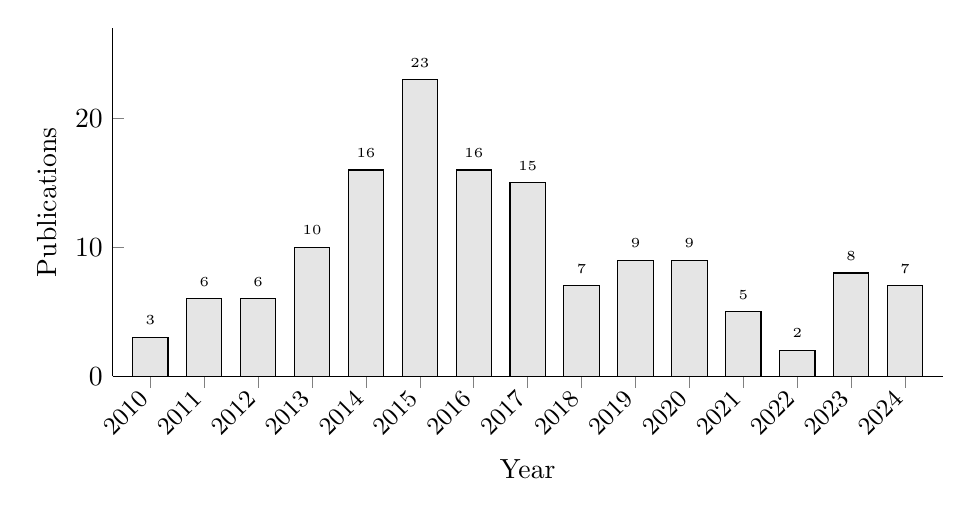
\begin{tikzpicture}
\begin{axis}[
    ybar,
    bar width=0.45cm,
    width=\textwidth,
    height=6cm,
    xlabel={Year},
    ylabel={Publications},
    ymin=0,
    ymax=27,
    xtick={2010,2011,2012,2013,2014,2015,2016,2017,2018,2019,2020,2021,2022,2023,2024},
    xticklabel style={rotate=45, anchor=east, font=\small, /pgf/number format/1000 sep={}},
    nodes near coords,
    nodes near coords style={font=\tiny, above},
    every node near coord/.append style={yshift=1pt},
    axis lines*=left,
    enlarge x limits=0.05,
]
\addplot[fill=gray!20, draw=black, line width=0.4pt] coordinates {
    (2010, 3)
    (2011, 6)
    (2012, 6)
    (2013, 10)
    (2014, 16)
    (2015, 23)
    (2016, 16)
    (2017, 15)
    (2018, 7)
    (2019, 9)
    (2020, 9)
    (2021, 5)
    (2022, 2)
    (2023, 8)
    (2024, 7)
};
\end{axis}
\end{tikzpicture}}
    \caption{Code-reuse attack and defense publications in security venues (IEEE S\&P, USENIX Security, CCS, NDSS, AsiaCCS, Euro S\&P) from 2010 to 2024.
    The paper metadata was retrieved from DBLP, and filtered using semantic clustering on titles and abstracts.
    The full list of papers is provided in \Cref{app:code-reuse-papers}.}
    \label{fig:intro:code-reuse-trend}
\end{figure}

A dominant class of exploits targeting these vulnerabilities is code-reuse attacks.
Attackers hijack a program's control flow and subsequently reuse existing code \enquote{gadgets} already present in the target process.
This approach allows attackers to bypass defenses like \wox, which, thanks to widespread hardware support, have become a de facto standard.
Over the years, different ways of defending against this type of attack have emerged.
One prominent defense category is randomization or more broadly, software diversity.
Software diversity embraces the possibility of memory corruptions and control-flow diversion and instead aims to restrict an attacker's mobility.
By introducing controlled randomness into code or data layouts, software diversity disrupts attackers’ assumptions.
For example, without knowing the exact location of functions or gadgets, an attacker can no longer use them in a code-reuse attack.
Unfortunately, closing all information channels an attacker could use to undermine the guarantees provided by randomization proves difficult in practice.
Recent work shows that even when code is perfectly hidden, predictable data structures such as the stack, global objects, or allocator metadata, can leak enough information for a successful attack~\cite{Rudd2017}.
The consequence is that although, judging by the publication counts, the security community's interest in code-reuse mitigations has declined, unsolved problems remain.
\Cref{fig:intro:code-reuse-trend} shows the number of code-reuse-related publications in top security venues from 2010 to 2024.
The figure clearly shows the peak interest around 2015--2016 and the subsequent decline.
While hardware defenses like Intel CET and ARM PAC have reduced the urgency for software-only solutions, they are not a silver bullet and research continues, particularly for embedded systems and attestation.
This trend is particularly worrying given the rapidly increasing capabilities of \gls{LLM}s with respect to offensive security.
Already in the year 2026, \gls{LLM}s can reduce the cost of creating highly sophisticated code-reuse exploits from days or even weeks down to a few hours and an investment of a few euros, and this is likely only the beginning~\cite{anthropic2026zerodays}.
At these drastically reduced costs, even sophisticated targeted attacks fall within the capabilities of non-state actors.
In light of these developments, we hope that the loss of interest in \glspl{CRA} is only temporary and that research on more capable defenses continues.
\section{Reliability}
Traditional approaches to software reliability, such as static analysis, unit testing, and formal verification, serve as the foundation of quality assurance.
While formal verification offers the strongest theoretical guarantees, it faces significant practical hurdles.
A key problem is often the lack of specification: verification requires properties to be formally defined, yet formulating such specifications is usually non-trivial.
Even when adequate specifications exist, the computational cost and limited scalability of formal methods prove prohibitive for large, evolving systems.
Similarly, static analysis faces inherent trade-offs between precision and scalability.
Finally, unit testing remains the most widespread technique but suffers from a critical blind spot: it is conceptually limited by human foresight and can only validate scenarios explicitly anticipated by the test author.

In light of these shortcomings, a long-neglected technique named fuzz testing, or fuzzing for short, has become increasingly important over the past 10--15 years.
This rise in popularity happened partly because of \propername{AFL}, a practical and fast fuzzer that combines code coverage feedback with carefully engineered heuristics.
Early fuzzers mostly relied on simple, random input generation and were often dismissed as crude or ad hoc.
Modern fuzzing, by contrast, combines feedback-guided input mutation and scheduling, constraint solving, and domain-specific generators to explore program behaviors more systematically.
Industrial-strength frameworks such as \aflpp, \propername{libFuzzer}, and their successors have demonstrated that fuzzing can uncover deep, previously unknown bugs in widely deployed software, including operating systems, browsers, cryptographic libraries, and compilers.

Most popular fuzzers like \aflpp and \propername{libFuzzer} rely on code coverage feedback to guide their mutation and scheduling decisions.
Despite its widespread use, code coverage is an imperfect proxy for test effectiveness, particularly for state-rich systems such as compilers.
Code coverage metrics---statement, branch, or edge coverage---abstract away the program’s internal state and treat all executions that follow the same control-flow paths as equivalent.
As a result, fuzzers can quickly saturate coverage while still failing to explore nuanced interactions within the same control-flow.
To find these deeper bugs, the fuzzer needs a better guide---one that considers more of the target program's internal state space.

%Meanwhile, the tools we use to build everything else—modern compilers, linkers, and virtual machines—have themselves grown complexity.
%Each new optimization pass, hardware backend, or language front-end enlarges the space of subtle interactions that manual review or unit tests rarely exercise, so bugs continue to slip through release pipelines.
%These observations are particularly true for \glspl{JIT}.
%\glspl{JIT} are typically part of a language VM and compile user-provided, potentially malicious code.
%When compiling such code, \glspl{JIT} are supposed to upkeep the sandboxing guarantees of the underlying language VM, such as enforcing array boundaries.
%As such, the correctness of \glspl{JIT} has an important security dimension as well.
%

\section{The Compiler's Role Beyond Optimization}
In this thesis I argue that compilers are uniquely positioned to help improve both software reliability and security.
Every non-trivial program passes through a compiler at some point, either ahead of time or just in time\footnote{Interpreted programs are an exception, but the interpreter itself has passed through a compiler as well.}.
Due to this compilation \enquote{bottleneck}, a single transformation deployed in the toolchain can harden millions of downstream binaries.

Compilers possess semantic insight that is hard, if not impossible, for post-compilation transformations to replicate.
The compiler's knowledge encompasses both programming language semantics and details about the target machine.
Compilers, for example, know the exact type hierarchy of compiled \cpp programs and the exact geometry of their stack frames.
While this information can be partially recovered from binaries, the reconstruction is notoriously challenging because compilation is a lossy process.
Similarly, compilers have detailed knowledge about the compilation process itself, such as which transformations were applied and which invariants justified those transformations.

In this thesis I explore how to tap these information sources for security hardening and improved fuzzing feedback.

\section{Structure}

This thesis presents three contributions that demonstrate the compiler's potential to improve software security and reliability.
The common thread is the compiler's unique vantage point: it possesses semantic knowledge about program structure that can be leveraged for purposes \emph{beyond optimization}.
The contributions are structured into two parts, with \cref{part:defense} focusing on security and \cref{part:fuzzing} on fuzzing.
Each part concludes with an \emph{Outlook} chapter that discusses more general ideas and possible future research directions.

\paragraph{R2C: Compiler-Driven Data Diversity}
In \cref{ch:r2c} I present \rtwoc, a novel software diversity defense that addresses the challenge of layout inference through information leaks.
Unlike prior work that focused primarily on code randomization, \rtwoc leverages the compiler's knowledge of stack frame geometry to randomize observable data layouts.
By disguising sensitive pointers among booby-trapped decoys, \rtwoc substantially raises reconnaissance cost while incurring moderate performance overhead.
While introducing new diversity techniques, \rtwoc also reveals the challenges diversity faces when subjected to targeted attacks with a powerful threat model.

\paragraph{LOOL: Optimization-Aware Compiler Fuzzing}
In \cref{ch:lool} I present \lool, a compiler fuzzing framework based on a new type of coverage feedback.
Instead of relying on code coverage, \lool leverages the compiler's own optimization log as a domain-specific feedback signal.
A genetic algorithm uses this feedback to steer test-case generation toward rare optimization interactions that are difficult to trigger otherwise.
Our suggested domain-specific coverage is both more efficient and targeted than code coverage.

\paragraph{Program State Projection}
In \cref{ch:psp} I present \emph{Program State Projection} (PSP), a technique that uses compiler analyses to expose hidden data dependencies to coverage-guided fuzzers.
By transforming indirect calls into explicit control-flow branches and partitioning value ranges, PSP aims to provide stepping stones that help fuzzers explore program states that conventional coverage metrics would conflate.
Although at present our evaluation shows no quantifiable gains in terms of code coverage and bug-finding performance, the broader \gls{PSP} framework reveals a new principle for supporting code-coverage-guided fuzzers.
\label{ch:introduction}

\partintro{%
Memory-unsafe languages like C and \cpp remain the foundation of critical infrastructure, and with them, the threat of memory corruption vulnerabilities persists.
Among the most dangerous exploitation techniques are \glspl{CRA}, which hijack a program's control flow to execute attacker-chosen code sequences.

This part of the thesis explores how compiler-driven software diversity can defend against such attacks.
The compiler's intimate knowledge of program structure---stack layouts, function boundaries, and data dependencies---enables transformations that would be difficult or impossible to achieve through post-hoc binary rewriting or runtime instrumentation.

\Cref{ch:code-reuse-coevolution} traces the co-evolution of \glspl{CRA} and their defenses, establishing the context for our contribution.
The subsequent chapter then presents \rtwoc, a defense that leverages compiler knowledge to randomize not only code but also the observable data layouts that recent attacks exploit for reconnaissance.
}
\part{Defending Against Code-Reuse with Compiler Assistance}\label{part:defense}
\chapter{The Co-Evolution of Code-Reuse Attacks and Defenses}\label{ch:code-reuse-coevolution}
The history of software security is characterized by a continuous cycle of new attack avenues and corresponding defensive responses.
This co-evolutionary process has led to a landscape of highly sophisticated memory corruption exploits and mitigations.
A particularly common and dangerous class of memory corruption exploits is \glspl{CRA} and their---now mostly obsolete---predecessor code-injection attacks.

Code-injection attacks and \glspl{CRA} typically proceed in three phases:
\begin{inline}
    \item a reconnaissance phase where the attacker collects information about the target, such as addresses of target code,
    \item a memory corruption to overwrite control-flow data and
    \item the malicious code execution that transfers control to attacker-chosen code.
\end{inline}
Defenses against such attacks fall into three categories:
\begin{itemize}
    \item memory-safety enforcement;
    \item control-flow enforcement;
    \item randomization.
\end{itemize}
Each defense category targets a different step of the attack.
Memory-safety enforcement aims to prevent the memory corruption required to divert the control flow.
Control-flow enforcement tolerates the memory corruption but tries to lock the attacker into a previously determined control-flow graph.
Randomization-based techniques, also called software diversity, aim to disrupt the attacker's reconnaissance phase by invalidating a priori knowledge the attacker has about the target.

Increasingly sophisticated \gls{CRA} variants have driven the evolution of defenses in each category.
The following sections trace the historical development of \glspl{CRA} together with the development of defenses in each category.
\cref{fig:coevolution-epoch-all} shows the complete timeline for important \glspl{CRA} and defenses and each of the following sections looks at an epoch in this timeline in more detail.



\begin{figure}[p]
    \centering
    \resizebox{!}{0.95\textheight}{%
        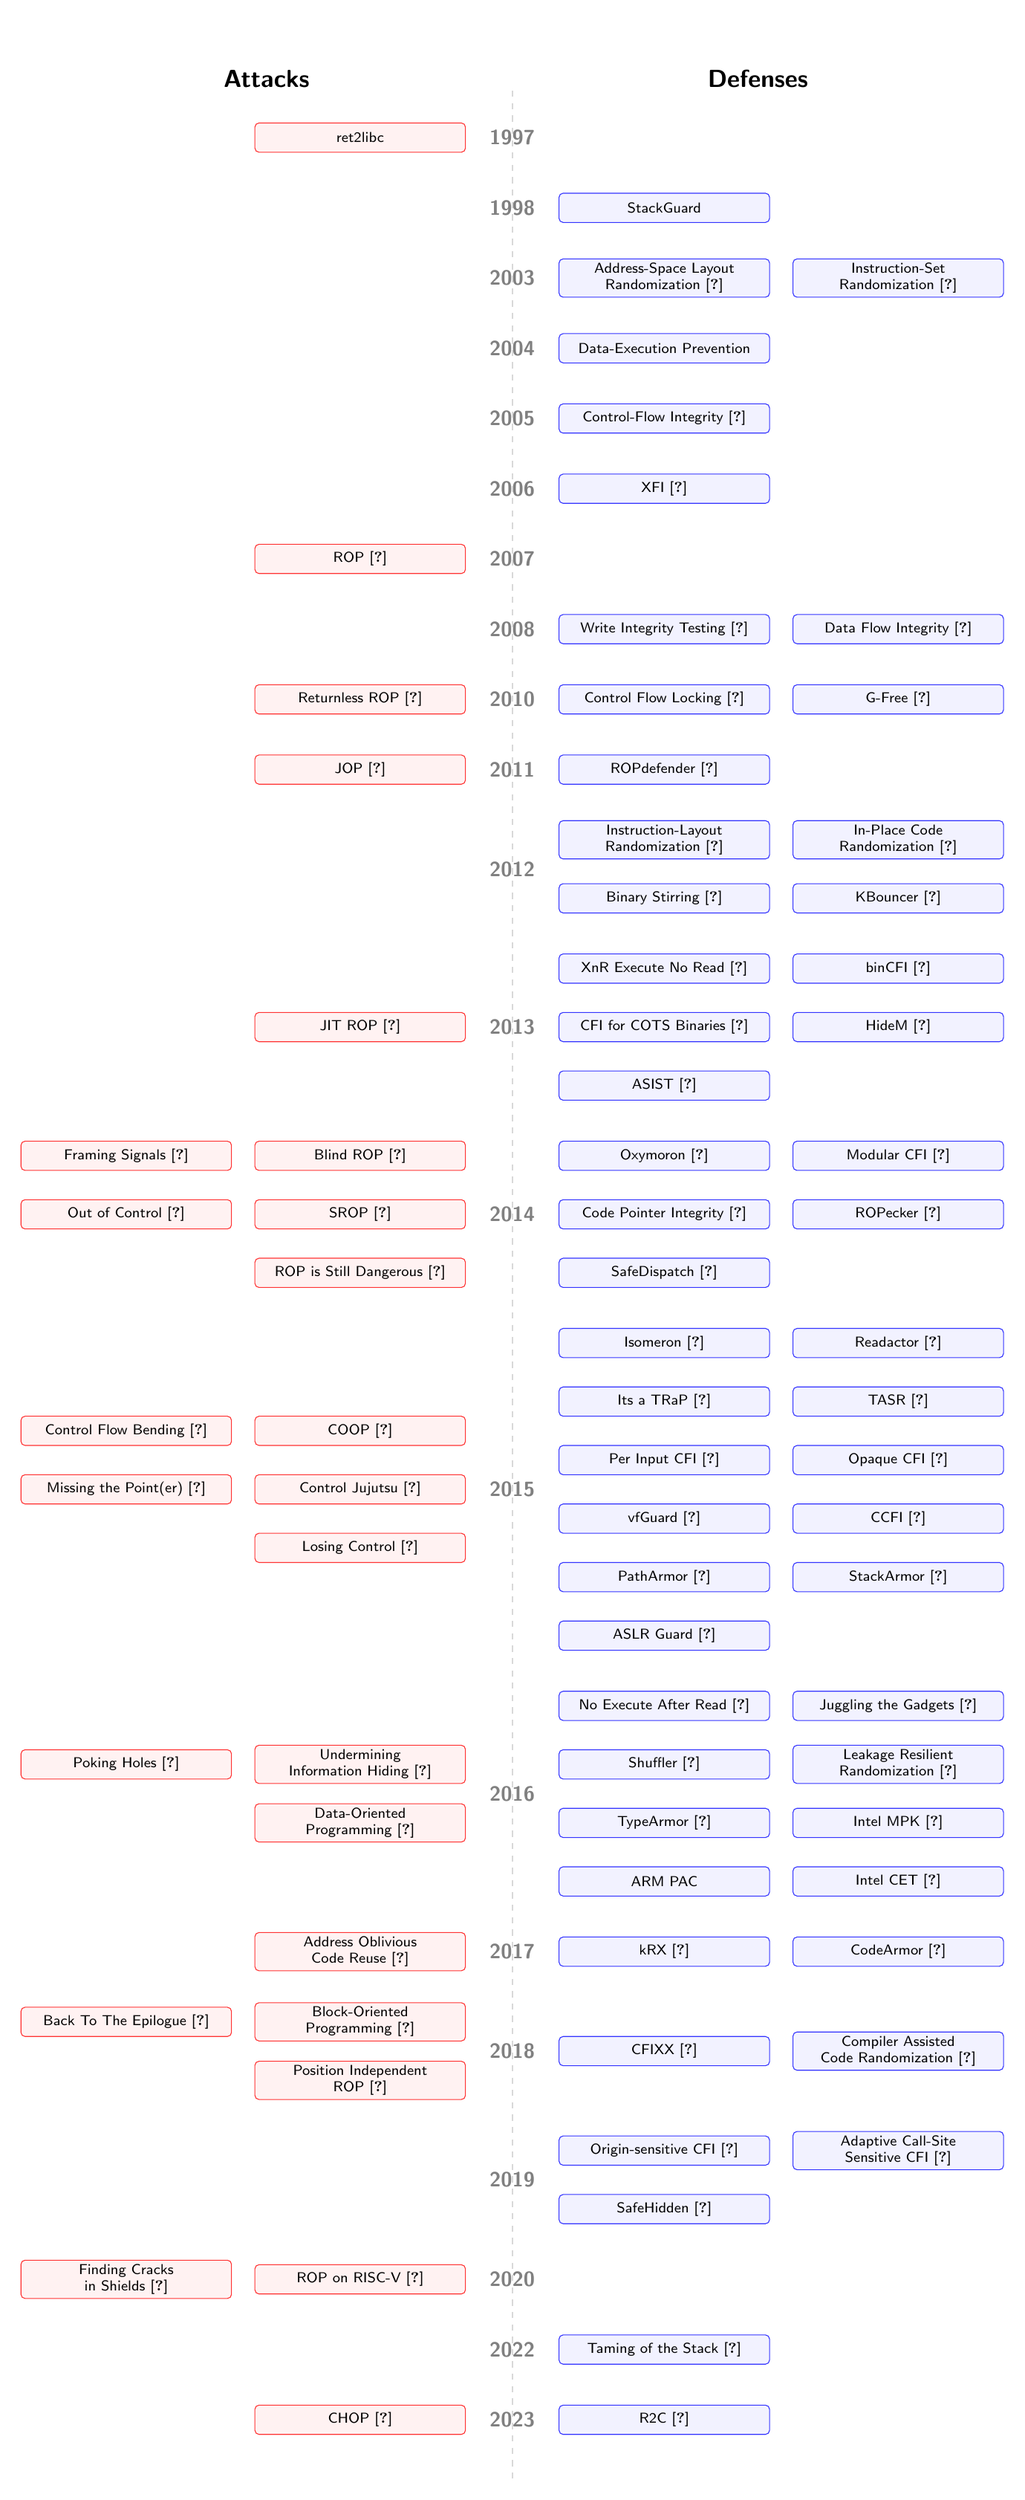
\begin{tikzpicture}[year node/.style={font=\bfseries\sffamily\color{gray}, align=center, inner sep=2pt},attack node/.style={draw=red!80, fill=red!5, rounded corners=2pt, font=\scriptsize\sffamily, align=center, minimum width=3.60cm, minimum height=0.5cm, inner sep=2pt, text width=3.40cm, execute at begin node=\setlength{\emergencystretch}{0pt}\tolerance 200\hyphenpenalty 10000\exhyphenpenalty 10000},defense node/.style={draw=blue!80, fill=blue!5, rounded corners=2pt, font=\scriptsize\sffamily, align=center, minimum width=3.60cm, minimum height=0.5cm, inner sep=2pt, text width=3.40cm, execute at begin node=\setlength{\emergencystretch}{0pt}\tolerance 200\hyphenpenalty 10000\exhyphenpenalty 10000},spine/.style={thick, gray!30, dashed}]%
\node[font=\large\bfseries\sffamily] at (-4.2,1.0) {Attacks};%
\node[font=\large\bfseries\sffamily] at (4.2,1.0) {Defenses};%
  % Year 1997%
\node[year node] at (0.0,0.0) {1997};%
\node[attack node] at (-2.6,0.0) {ret2libc};%
  % Year 1998%
\node[year node] at (0.0,-1.2) {1998};%
\node[defense node] at (2.6,-1.2) {StackGuard};%
  % Year 2003%
\node[year node] at (0.0,-2.4) {2003};%
\node[defense node] at (2.6,-2.4) {Address{-}Space Layout\\ Randomization \allowbreak\cite{PaXTeam2003}};%
\node[defense node] at (6.6,-2.4) {Instruction{-}Set\\ Randomization \allowbreak\cite{boyd2010}};%
  % Year 2004%
\node[year node] at (0.0,-3.6) {2004};%
\node[defense node] at (2.6,-3.6) {Data{-}Execution Prevention};%
  % Year 2005%
\node[year node] at (0.0,-4.8) {2005};%
\node[defense node] at (2.6,-4.8) {Control{-}Flow Integrity \allowbreak\cite{Abadi2005}};%
  % Year 2006%
\node[year node] at (0.0,-6.0) {2006};%
\node[defense node] at (2.6,-6.0) {XFI \allowbreak\cite{Erlingsson2006}};%
  % Year 2007%
\node[year node] at (0.0,-7.2) {2007};%
\node[attack node] at (-2.6,-7.2) {ROP \allowbreak\cite{Shacham2007}};%
  % Year 2008%
\node[year node] at (0.0,-8.4) {2008};%
\node[defense node] at (2.6,-8.4) {Write Integrity Testing \allowbreak\cite{Akritidis2008}};%
\node[defense node] at (6.6,-8.4) {Data Flow Integrity \allowbreak\cite{castro2006}};%
  % Year 2010%
\node[year node] at (0.0,-9.6) {2010};%
\node[attack node] at (-2.6,-9.6) {Returnless ROP \allowbreak\cite{checkoway2010}};%
\node[defense node] at (2.6,-9.6) {Control Flow Locking \allowbreak\cite{Bletsch2011b}};%
\node[defense node] at (6.6,-9.6) {G{-}Free \allowbreak\cite{Onarlioglu2010}};%
  % Year 2011%
\node[year node] at (0.0,-10.8) {2011};%
\node[attack node] at (-2.6,-10.8) {JOP \allowbreak\cite{Bletsch2011a}};%
\node[defense node] at (2.6,-10.8) {ROPdefender \allowbreak\cite{davi2011}};%
  % Year 2012%
\node[year node] at (0.0,-12.5) {2012};%
\node[defense node] at (2.6,-12.0) {Instruction{-}Layout\\ Randomization \allowbreak\cite{Hiser2012}};%
\node[defense node] at (6.6,-12.0) {In{-}Place Code\\ Randomization \allowbreak\cite{Pappas2012a}};%
\node[defense node] at (2.6,-13.0) {Binary Stirring \allowbreak\cite{Wartell2012}};%
\node[defense node] at (6.6,-13.0) {KBouncer \allowbreak\cite{Pappas2013b}};%
  % Year 2013%
\node[year node] at (0.0,-15.2) {2013};%
\node[attack node] at (-2.6,-15.2) {JIT ROP \allowbreak\cite{Snow2013}};%
\node[defense node] at (2.6,-14.2) {XnR Execute No Read \allowbreak\cite{Backes2013}};%
\node[defense node] at (6.6,-14.2) {binCFI \allowbreak\cite{zhang2013}};%
\node[defense node] at (2.6,-15.2) {CFI for COTS Binaries \allowbreak\cite{zhang2013}};%
\node[defense node] at (6.6,-15.2) {HideM \allowbreak\cite{Goktas2016b}};%
\node[defense node] at (2.6,-16.2) {ASIST \allowbreak\cite{papadogiannakis2013}};%
  % Year 2014%
\node[year node] at (0.0,-18.4) {2014};%
\node[attack node] at (-2.6,-17.4) {Blind ROP \allowbreak\cite{Bittau2014a}};%
\node[attack node] at (-6.6,-17.4) {Framing Signals \allowbreak\cite{Bittau2014a}};%
\node[attack node] at (-2.6,-18.4) {SROP \allowbreak\cite{bosman2014}};%
\node[attack node] at (-6.6,-18.4) {Out of Control \allowbreak\cite{Goktas2016b}};%
\node[attack node] at (-2.6,-19.4) {ROP is Still Dangerous \allowbreak\cite{carlini2014}};%
\node[defense node] at (2.6,-17.4) {Oxymoron \allowbreak\cite{Backes2014f}};%
\node[defense node] at (6.6,-17.4) {Modular CFI \allowbreak\cite{niu2014}};%
\node[defense node] at (2.6,-18.4) {Code Pointer Integrity \allowbreak\cite{Kuznetsov2014}};%
\node[defense node] at (6.6,-18.4) {ROPecker \allowbreak\cite{Cheng2014}};%
\node[defense node] at (2.6,-19.4) {SafeDispatch \allowbreak\cite{jang2014}};%
  % Year 2015%
\node[year node] at (0.0,-23.1) {2015};%
\node[attack node] at (-2.6,-22.1) {COOP \allowbreak\cite{Schuster2015a}};%
\node[attack node] at (-6.6,-22.1) {Control Flow Bending \allowbreak\cite{Carlini2015}};%
\node[attack node] at (-2.6,-23.1) {Control Jujutsu \allowbreak\cite{Evans2015a}};%
\node[attack node] at (-6.6,-23.1) {Missing the Point(er) \allowbreak\cite{Evans2015}};%
\node[attack node] at (-2.6,-24.1) {Losing Control \allowbreak\cite{conti2015}};%
\node[defense node] at (2.6,-20.6) {Isomeron \allowbreak\cite{Davi2015}};%
\node[defense node] at (6.6,-20.6) {Readactor \allowbreak\cite{Crane2015}};%
\node[defense node] at (2.6,-21.6) {Its a TRaP \allowbreak\cite{Crane2015b}};%
\node[defense node] at (6.6,-21.6) {TASR \allowbreak\cite{bigelow2015}};%
\node[defense node] at (2.6,-22.6) {Per Input CFI \allowbreak\cite{Niu2015}};%
\node[defense node] at (6.6,-22.6) {Opaque CFI \allowbreak\cite{Mohan2015}};%
\node[defense node] at (2.6,-23.6) {vfGuard \allowbreak\cite{Prakash2015}};%
\node[defense node] at (6.6,-23.6) {CCFI \allowbreak\cite{Mashtizadeh2015}};%
\node[defense node] at (2.6,-24.6) {PathArmor \allowbreak\cite{Goktas2016b}};%
\node[defense node] at (6.6,-24.6) {StackArmor \allowbreak\cite{Chen2015c}};%
\node[defense node] at (2.6,-25.6) {ASLR Guard \allowbreak\cite{Lu2015}};%
  % Year 2016%
\node[year node] at (0.0,-28.3) {2016};%
\node[attack node] at (-2.6,-27.8) {Undermining\\ Information Hiding \allowbreak\cite{Goktas2016}};%
\node[attack node] at (-6.6,-27.8) {Poking Holes \allowbreak\cite{Oikonomopoulos2016a}};%
\node[attack node] at (-2.6,-28.8) {Data{-}Oriented\\ Programming \allowbreak\cite{Hu2016}};%
\node[defense node] at (2.6,-26.8) {No Execute After Read \allowbreak\cite{Werner2016}};%
\node[defense node] at (6.6,-26.8) {Juggling the Gadgets \allowbreak\cite{koo2016}};%
\node[defense node] at (2.6,-27.8) {Shuffler \allowbreak\cite{WilliamsKing2016}};%
\node[defense node] at (6.6,-27.8) {Leakage Resilient\\ Randomization \allowbreak\cite{Braden2016}};%
\node[defense node] at (2.6,-28.8) {TypeArmor \allowbreak\cite{VanderVeen2015b}};%
\node[defense node] at (6.6,-28.8) {Intel MPK \allowbreak\cite{Wahbe1993}};%
\node[defense node] at (2.6,-29.8) {ARM PAC};%
\node[defense node] at (6.6,-29.8) {Intel CET \allowbreak\cite{IntelCET}};%
  % Year 2017%
\node[year node] at (0.0,-31.0) {2017};%
\node[attack node] at (-2.6,-31.0) {Address Oblivious\\ Code Reuse \allowbreak\cite{Rudd2017}};%
\node[defense node] at (2.6,-31.0) {kRX \allowbreak\cite{Pomonis2019}};%
\node[defense node] at (6.6,-31.0) {CodeArmor \allowbreak\cite{Chen2017a}};%
  % Year 2018%
\node[year node] at (0.0,-32.7) {2018};%
\node[attack node] at (-2.6,-32.2) {Block{-}Oriented\\ Programming \allowbreak\cite{Ispoglou2018}};%
\node[attack node] at (-6.6,-32.2) {Back To The Epilogue \allowbreak\cite{biondo2018}};%
\node[attack node] at (-2.6,-33.2) {Position Independent\\ ROP \allowbreak\cite{Goktas2018}};%
\node[defense node] at (2.6,-32.7) {CFIXX \allowbreak\cite{Burow2018CFIXX}};%
\node[defense node] at (6.6,-32.7) {Compiler Assisted\\ Code Randomization \allowbreak\cite{Koo2018}};%
  % Year 2019%
\node[year node] at (0.0,-34.9) {2019};%
\node[defense node] at (2.6,-34.4) {Origin{-}sensitive CFI \allowbreak\cite{khandaker2019}};%
\node[defense node] at (6.6,-34.4) {Adaptive Call{-}Site\\ Sensitive CFI \allowbreak\cite{khandaker2019a}};%
\node[defense node] at (2.6,-35.4) {SafeHidden \allowbreak\cite{wang2019a}};%
  % Year 2020%
\node[year node] at (0.0,-36.6) {2020};%
\node[attack node] at (-2.6,-36.6) {ROP on RISC{-}V \allowbreak\cite{jaloyan2020}};%
\node[attack node] at (-6.6,-36.6) {Finding Cracks\\ in Shields \allowbreak\cite{li2020}};%
  % Year 2022%
\node[year node] at (0.0,-37.8) {2022};%
\node[defense node] at (2.6,-37.8) {Taming of the Stack \allowbreak\cite{huang2022a}};%
  % Year 2023%
\node[year node] at (0.0,-39.0) {2023};%
\node[attack node] at (-2.6,-39.0) {CHOP \allowbreak\cite{duta2023}};%
\node[defense node] at (2.6,-39.0) {R2C \allowbreak\cite{berlakovich2023}};%
\path[spine,draw] (0.0,0.8) -- (0.0,-40.0);%
\path[use as bounding box] (-8.40,-40.00) rectangle (8.40,2.00);%
\end{tikzpicture}%
    }
    \caption{Timeline for code-injection attacks and defenses (1997--Present).}
    \label{fig:coevolution-epoch-all}
\end{figure}


\FloatBarrier
\begin{figure}[H]
    \centering
    \resizebox{\textwidth}{!}{%
        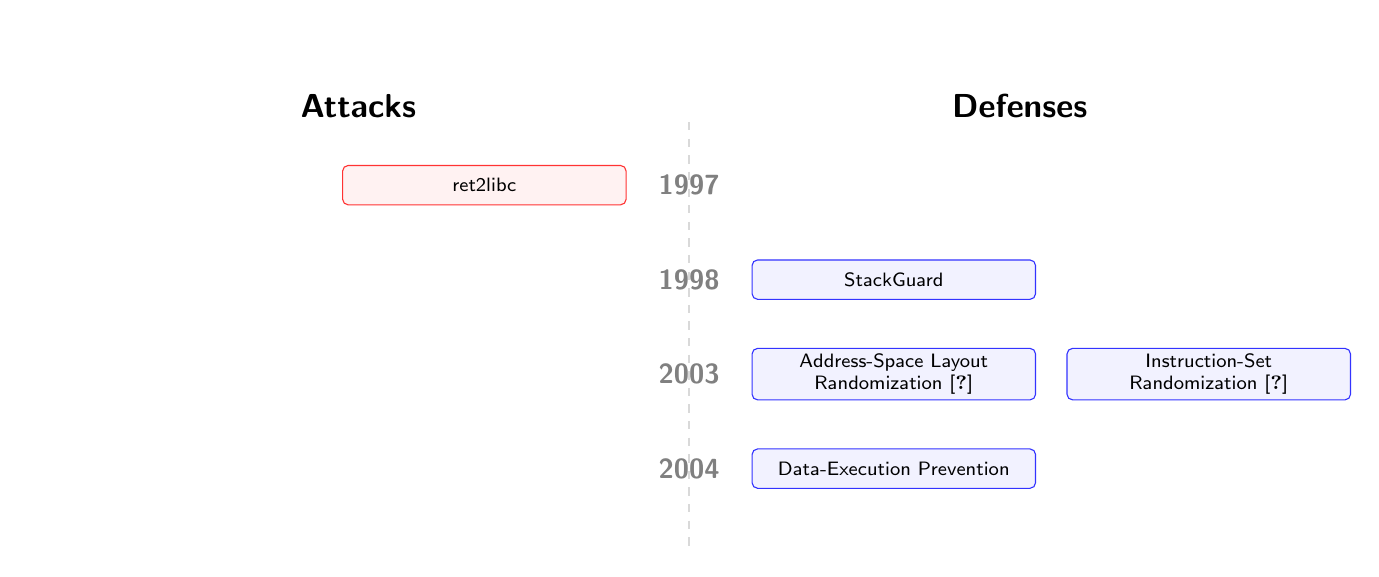
\begin{tikzpicture}[year node/.style={font=\bfseries\sffamily\color{gray}, align=center, inner sep=2pt},attack node/.style={draw=red!80, fill=red!5, rounded corners=2pt, font=\scriptsize\sffamily, align=center, minimum width=3.60cm, minimum height=0.5cm, inner sep=2pt, text width=3.40cm, execute at begin node=\setlength{\emergencystretch}{0pt}\tolerance 200\hyphenpenalty 10000\exhyphenpenalty 10000},defense node/.style={draw=blue!80, fill=blue!5, rounded corners=2pt, font=\scriptsize\sffamily, align=center, minimum width=3.60cm, minimum height=0.5cm, inner sep=2pt, text width=3.40cm, execute at begin node=\setlength{\emergencystretch}{0pt}\tolerance 200\hyphenpenalty 10000\exhyphenpenalty 10000},spine/.style={thick, gray!30, dashed}]%
\node[font=\large\bfseries\sffamily] at (-4.2,1.0) {Attacks};%
\node[font=\large\bfseries\sffamily] at (4.2,1.0) {Defenses};%
  % Year 1997%
\node[year node] at (0.0,0.0) {1997};%
\node[attack node] at (-2.6,0.0) {ret2libc};%
  % Year 1998%
\node[year node] at (0.0,-1.2) {1998};%
\node[defense node] at (2.6,-1.2) {StackGuard};%
  % Year 2003%
\node[year node] at (0.0,-2.4) {2003};%
\node[defense node] at (2.6,-2.4) {Address{-}Space Layout\\ Randomization \allowbreak\cite{PaXTeam2003}};%
\node[defense node] at (6.6,-2.4) {Instruction{-}Set\\ Randomization \allowbreak\cite{boyd2010}};%
  % Year 2004%
\node[year node] at (0.0,-3.6) {2004};%
\node[defense node] at (2.6,-3.6) {Data{-}Execution Prevention};%
\path[spine,draw] (0.0,0.8) -- (0.0,-4.6);%
\path[use as bounding box] (-8.40,-4.60) rectangle (8.40,2.00);%
\end{tikzpicture}%
    }
    \caption{Epoch timeline for code-injection attacks and defenses (1997--2004).}
    \label{fig:coevolution-epoch-code-injection}
\end{figure}
\section{Code Injection (1997--2004)}
\label{sec:epoch-injection}
In the earliest era (1997--2004), the adversary's primary goal was to inject new code (\eg shellcode) into the target process' memory space and subsequently redirect execution to the injected code.
Despite the possibility of code injection in the early days, a form of \gls{CRA} called \propername{return-to-libc} was described already in 1997.
\propername{Return-to-libc} operates on the function level and reuses functions from the standard C library.
These functions are both powerful and likely present in most attacked programs.

To counter these early attacks, several randomization-based techniques were proposed.
\propername{StackGuard} protects return addresses against buffer overflows with \enquote{canaries}---random values checked before a function returns.
Based on the observation that an attacker needs exact addresses both for injection and reuse, \gls{ASLR} was introduced to randomize the base addresses of the stack, heap and libraries~\cite{PaXTeam2003}.
Full adoption of \gls{ASLR} took years, however, as it requires position-independent code.
Another issue with \gls{ASLR} is that a 32-bit address space does not offer enough entropy, and even in a 64-bit address space, pointer leaks and side-channels make \gls{ASLR} vulnerable~\cite{Gras2017}.
Even ten years later, \gls{ASLR} implementations still suffer from severe limitations~\cite{binosi2024}.
Research into \gls{ISR} explored randomizing the processor's instruction set to prevent the execution of injected code~\cite{boyd2010,papadogiannakis2013}.

At around 2004, the introduction of a new \gls{CPU} feature made it practical to prevent memory regions from being writable and executable at the same time.
The memory-safety enforcement mechanism leveraging this \gls{CPU} feature is known as \wox or \gls{DEP}.
With the widespread adoption of \gls{DEP}, attackers were forced to switch to more advanced forms of \glspl{CRA}.

\FloatBarrier
\begin{figure}[H]
    \centering
    \resizebox{\textwidth}{!}{%
        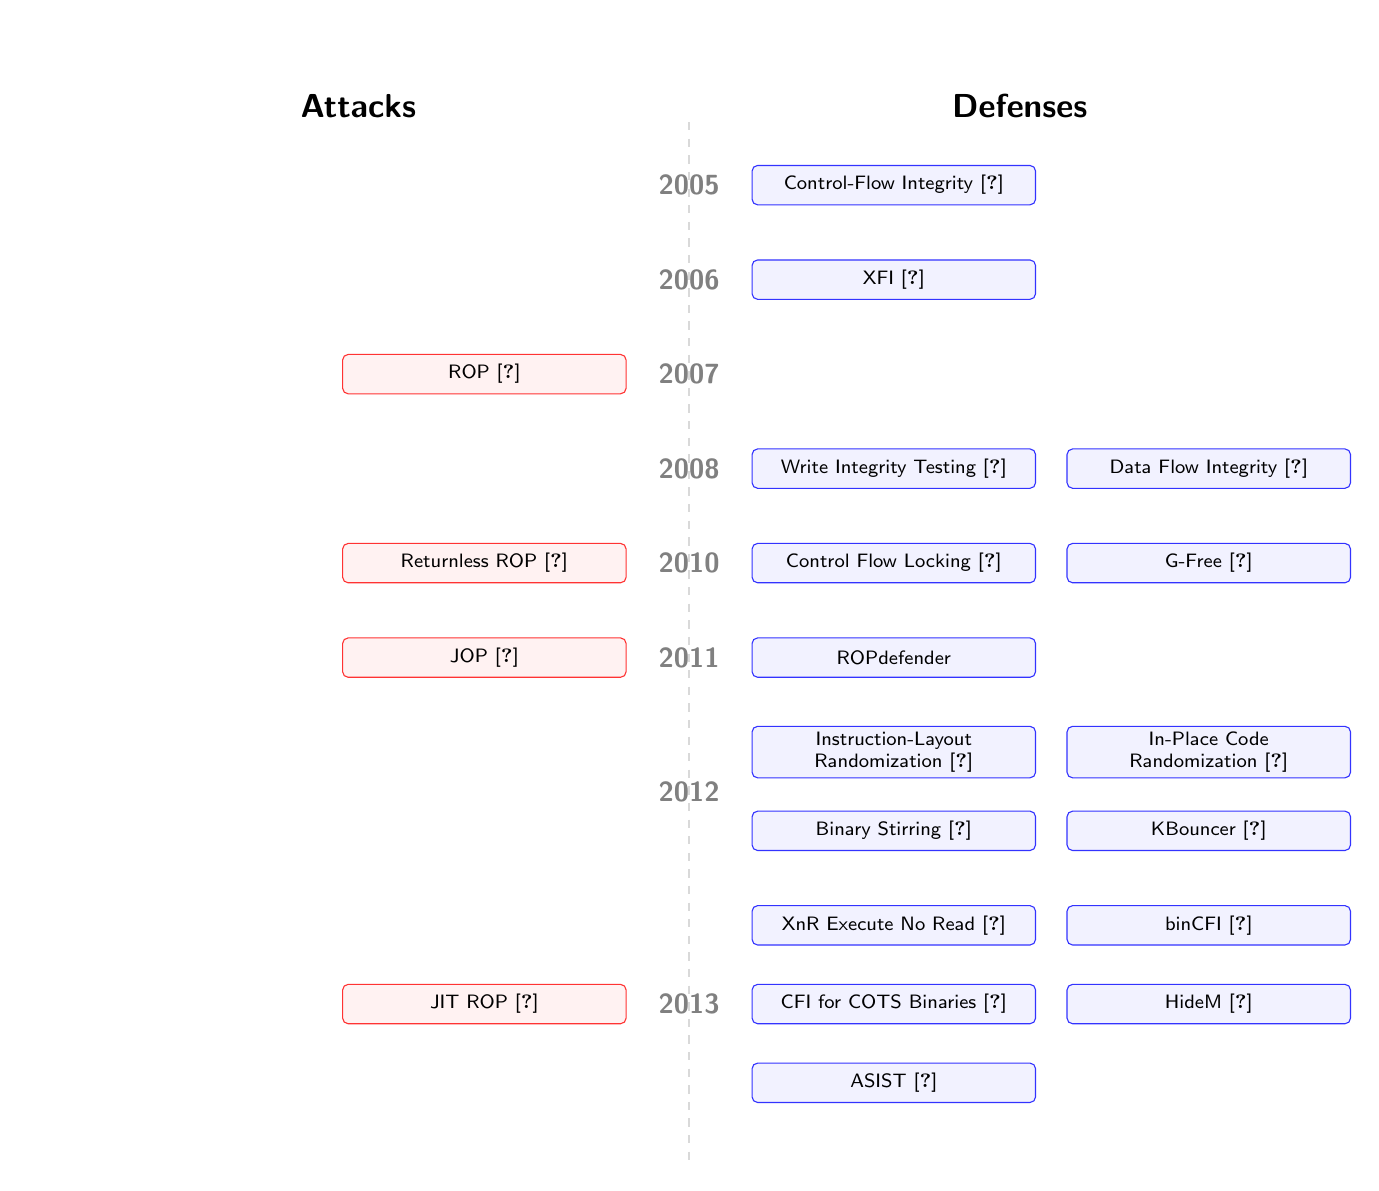
\begin{tikzpicture}[year node/.style={font=\bfseries\sffamily\color{gray}, align=center, inner sep=2pt},attack node/.style={draw=red!80, fill=red!5, rounded corners=2pt, font=\scriptsize\sffamily, align=center, minimum width=3.60cm, minimum height=0.5cm, inner sep=2pt, text width=3.40cm, execute at begin node=\setlength{\emergencystretch}{0pt}\tolerance 200\hyphenpenalty 10000\exhyphenpenalty 10000},defense node/.style={draw=blue!80, fill=blue!5, rounded corners=2pt, font=\scriptsize\sffamily, align=center, minimum width=3.60cm, minimum height=0.5cm, inner sep=2pt, text width=3.40cm, execute at begin node=\setlength{\emergencystretch}{0pt}\tolerance 200\hyphenpenalty 10000\exhyphenpenalty 10000},spine/.style={thick, gray!30, dashed}]%
\node[font=\large\bfseries\sffamily] at (-4.2,1.0) {Attacks};%
\node[font=\large\bfseries\sffamily] at (4.2,1.0) {Defenses};%
  % Year 2005%
\node[year node] at (0.0,0.0) {2005};%
\node[defense node] at (2.6,0.0) {Control{-}Flow Integrity \allowbreak\cite{Abadi2005}};%
  % Year 2006%
\node[year node] at (0.0,-1.2) {2006};%
\node[defense node] at (2.6,-1.2) {XFI \allowbreak\cite{Erlingsson2006}};%
  % Year 2007%
\node[year node] at (0.0,-2.4) {2007};%
\node[attack node] at (-2.6,-2.4) {ROP \allowbreak\cite{Shacham2007}};%
  % Year 2008%
\node[year node] at (0.0,-3.6) {2008};%
\node[defense node] at (2.6,-3.6) {Write Integrity Testing \allowbreak\cite{Akritidis2008}};%
\node[defense node] at (6.6,-3.6) {Data Flow Integrity \allowbreak\cite{castro2006}};%
  % Year 2010%
\node[year node] at (0.0,-4.8) {2010};%
\node[attack node] at (-2.6,-4.8) {Returnless ROP \allowbreak\cite{checkoway2010}};%
\node[defense node] at (2.6,-4.8) {Control Flow Locking \allowbreak\cite{Bletsch2011b}};%
\node[defense node] at (6.6,-4.8) {G{-}Free \allowbreak\cite{Onarlioglu2010}};%
  % Year 2011%
\node[year node] at (0.0,-6.0) {2011};%
\node[attack node] at (-2.6,-6.0) {JOP \allowbreak\cite{Bletsch2011a}};%
\node[defense node] at (2.6,-6.0) {ROPdefender};%
  % Year 2012%
\node[year node] at (0.0,-7.7) {2012};%
\node[defense node] at (2.6,-7.2) {Instruction{-}Layout\\ Randomization \allowbreak\cite{Hiser2012}};%
\node[defense node] at (6.6,-7.2) {In{-}Place Code\\ Randomization \allowbreak\cite{Pappas2012a}};%
\node[defense node] at (2.6,-8.2) {Binary Stirring \allowbreak\cite{Wartell2012}};%
\node[defense node] at (6.6,-8.2) {KBouncer \allowbreak\cite{Pappas2013b}};%
  % Year 2013%
\node[year node] at (0.0,-10.4) {2013};%
\node[attack node] at (-2.6,-10.4) {JIT ROP \allowbreak\cite{Snow2013}};%
\node[defense node] at (2.6,-9.4) {XnR Execute No Read \allowbreak\cite{Backes2013}};%
\node[defense node] at (6.6,-9.4) {binCFI \allowbreak\cite{zhang2013}};%
\node[defense node] at (2.6,-10.4) {CFI for COTS Binaries \allowbreak\cite{zhang2013}};%
\node[defense node] at (6.6,-10.4) {HideM \allowbreak\cite{Goktas2016b}};%
\node[defense node] at (2.6,-11.4) {ASIST \allowbreak\cite{papadogiannakis2013}};%
\path[spine,draw] (0.0,0.8) -- (0.0,-12.4);%
\path[use as bounding box] (-8.40,-12.40) rectangle (8.40,2.00);%
\end{tikzpicture}%
    }
    \caption{Epoch timeline for static return-oriented programming and defenses (2005--2013).}
    \label{fig:coevolution-epoch-static-rop}
\end{figure}
\section{Static Return-Oriented Programming (2005--2013)}
\label{sec:epoch-static-reuse}
With \gls{DEP} preventing code injection (mid-2000s), attackers were forced to change tactics.
As demonstrated by \propername{return-to-libc} already, reusing code already present in the process memory provides a viable alternative to injection.
In 2007, \citeauthor{Shacham2007} introduced the first version of \gls{ROP} attacks~\cite{Shacham2007}, a generalization of whole-function reuse attacks such as \propername{return-to-libc}.
\gls{ROP} attacks reuse small snippets of assembly that are already present in the target process and end in a free-branch instruction.
These snippets are commonly referred to as \emph{gadgets} and by chaining them into a \emph{gadget chain}, an attacker can achieve arbitrary code execution.
Initially, \citeauthor{Shacham2007} demonstrated \gls{ROP} for the x86 architecture and with gadgets ending in \code{ret} instructions.
\gls{ROP} was later generalized to other architectures~\cite{roemer2012,cloosters2022,jaloyan2020} and to alternative dispatch mechanisms~\cite{checkoway2010,Bletsch2011a,bosman2014}.

To prevent control-flow hijacking in general and \gls{ROP} in particular, researchers proposed to enforce the program's intended control-flow graph (\gls{CFG}).
\gls{CFI} aims to restrict control-flow transfers at runtime to the ones intended by the programmer for a particular program point and for a particular program state.
\begin{listing}
    \begin{minted}[escapeinside=||]{C}
int dispatch(short param) {
  void (*targets[])(void) = { func1, func2 };
  if (param > 3) {
    targets[0]();
  }
  |...|
}
    \end{minted}
    \label{r2c:lst:indirect-call-c}
    \caption{Example function in C with an indirect function call depending on a parameter.}
\end{listing}
For example, the indirect function call in \cref{r2c:lst:indirect-call-c} is supposed to happen only if \code{param > 3} and only ever to target \code{func1}.
Enforcing these ideal policies in practice proves to be challenging, which is why the majority of \gls{CFI} solutions focus on control-flow alone, ignoring the dataflow (\eg \code{param > 3}).

The first publication on \acrfull{CFI} appeared in \citeyear{Abadi2005}~\cite{Abadi2005}, actually predating the first \gls{ROP} publication~\cite{Shacham2007}.
Although the paper was publicly available, the implementation itself remained proprietary to Microsoft Research, which hindered its immediate adoption and prompted further research into open-source alternatives.
One such alternative was \propername{XFI} (2006), which used binary rewriting and verification to enforce \gls{CFI} on system address spaces~\cite{Erlingsson2006}.
A simple approach to \gls{CFI} is to limit \code{call} and \code{ret} instructions to the semantics typically used by compilers~\cite{Cheng2014}.
That is, \code{call} instructions are only used to jump to the beginning of a \emph{function} and \code{ret} instructions only jump to \emph{call-preceded} locations.
While this approach is relatively easy to implement and does not depend on precise static analysis, its defensive power is limited~\cite{Davi2014}.
Implementations like \enquote{CFI for COTS Binaries} and \enquote{ROPdefender} demonstrated that such policies could be applied to stripped binaries using static binary rewriting or instrumentation, albeit with the aforementioned precision limitations~\cite{zhang2013,davi2011}.
Another approach is to determine the program's \gls{CFG} via static analysis, to the extent possible.
Several \gls{CFI} implementations use a statically determined \gls{CFG} to restrict indirect calls (forward-edge control-flow transfers)~\cite{Abadi2005,ghaffarinia2019,niu2014,Mohan2015,Niu2015}.
Statically determining the \gls{CFG} has theoretical limits, however, and to avoid false positives, static \gls{CFI} solutions overapproximate possible targets~\cite{Grove2001a}.
To reduce the resulting attack surface, \enquote{Control-Flow Locking} refines the \gls{CFI} policy by dynamically locking and unlocking allowed targets~\cite{Bletsch2011b}.
Other approaches like \propername{G-Free} avoid the \gls{CFG} problem entirely by eliminating unaligned free branches during compilation, effectively removing the gadgets themselves~\cite{Onarlioglu2010}.
Using hardware features, \propername{kBouncer} utilizes the \gls{LBR} to check for \gls{ROP}-like execution patterns at runtime without requiring binary instrumentation~\cite{Pappas2013b}.

In contrast to \gls{CFI}, memory-safety techniques try to solve the problem at the root of many attack classes, including \glspl{CRA}: memory corruption.
Different memory-safety enforcement techniques restrict combinations of \enquote{who} (subject) is allowed to read or write \enquote{what} (spatial safety) and \enquote{when} (temporal safety).
For example, data-flow integrity~\cite{castro2006} and WIT~\cite{Akritidis2008} treat \emph{instructions} as subject and limit which memory objects each write-instruction is allowed to modify.
Both use static dataflow analysis to establish relations between instructions and allowed memory targets.
Other approaches treat \emph{pointers} as access control subjects and associate metadata with memory objects~\cite{Nagarakatte2009}.
The associated metadata can include the memory object bounds, type, and liveness information.
Upon accessing a memory object via a pointer, the enforcement techniques check the intended access against the valid object's metadata.
However, the major drawback of these precise memory-enforcement techniques is their often prohibitive performance overhead.
For example, combining \propername{SoftBounds} and \propername{CETS} for spatial and temporal safety leads to an overhead of more than 100\%~\cite{Nagarakatte2009}.

In the \gls{ROP} attacks from this era, collecting gadgets happens offline and before the actual attack, typically on a separate copy of the target binary.
For example, a \gls{ROP} attack requires the exact memory addresses of the gadgets used in an attack.
Offline gadget collection with an identical copy of the target is possible due to the software monoculture~\cite{Larsen2014}.
That is, in a non-diversified binary, an attacker can assume that all gadget locations are identical to their own installation of the target software~\cite{Cohen1993,Franz2010,Pappas2012a,Hiser2012,Larsen2014,Homescu2013a,Koo2018}.
In other words, an attacker knows \emph{a priori} where to find gadgets in the target process.
Randomization-based defenses attempt to invalidate this a priori knowledge an attacker has.
Such randomization techniques typically work at a finer granularity than \gls{ASLR}.
In-place code randomization invalidates knowledge about \gls{ROP} \emph{gadgets} by replacing instruction sequences with semantically equivalent instructions (\eg swapping registers)~\cite{Pappas2012a}.
Instruction-Layout randomization invalidates knowledge about gadget \emph{locations} by running the program in a custom virtual machine to randomize the location of every instruction~\cite{Hiser2012}.
Binary Stirring performs randomization on a basic-block level by shuffling basic blocks at load time~\cite{Wartell2012}.
\enquote{Juggling the Gadgets} explored function-level randomization with a focus on displacing gadgets to break gadget chains~\cite{koo2016}.
To make randomization more practical for deployment, \enquote{Compiler-Assisted Code Randomization} proposed embedding metadata into binaries to allow basic-block-level randomization without heavy runtime overhead~\cite{Koo2018}.
\cref{tab:randomization-granularity} contrasts different levels of randomization with the types of attacks they can prevent.

\begin{table}[t]
    \centering
    \caption{Comparison of randomization granularities.}
    \label{tab:randomization-granularity}
    \footnotesize
    \begin{thesistable}{
        colspec = {l l l l},
        headrows = 1,
    }
        \toprule
        \textbf{Technique} & \textbf{Granularity} & \textbf{Prevents} & \textbf{Limitation} \\
        \midrule
        \gls{ASLR} & Base Address & Static Exploit Reuse & Vulnerable to leaks; Low entropy (32-bit) \\
        Function Perm. & Function & Function Reuse & Vulnerable to \gls{ROP}; Partial overwrites \\
        Basic Block & Basic Block & \gls{ROP} Gadget Chains & Performance overhead \\
        Instruction & Instruction & All \gls{ROP} Gadgets & High overhead; Compatibility issues \\
        \bottomrule
    \end{thesistable}
\end{table}

%A crucial factor for the security of code randomization is the granularity of randomization.
%Thus, code-randomization techniques typically provide finer-grained randomization, such as function permutation~\cite{Kil2006,WilliamsKing2016,Braden2016,Chen2017a}, basic-block shuffling~\cite{Wartell2012,Mohan2015,Pomonis2017,Koo2018}, or instruction-level and register randomization~\cite{Kc2003,Pappas2012a,Braden2016,Crane2015,Crane2015b,Hiser2012,Kooa}.

\FloatBarrier
\begin{figure}[H]
    \centering
    \resizebox{0.95\textwidth}{!}{%
        \resizebox{\textwidth}{!}{%
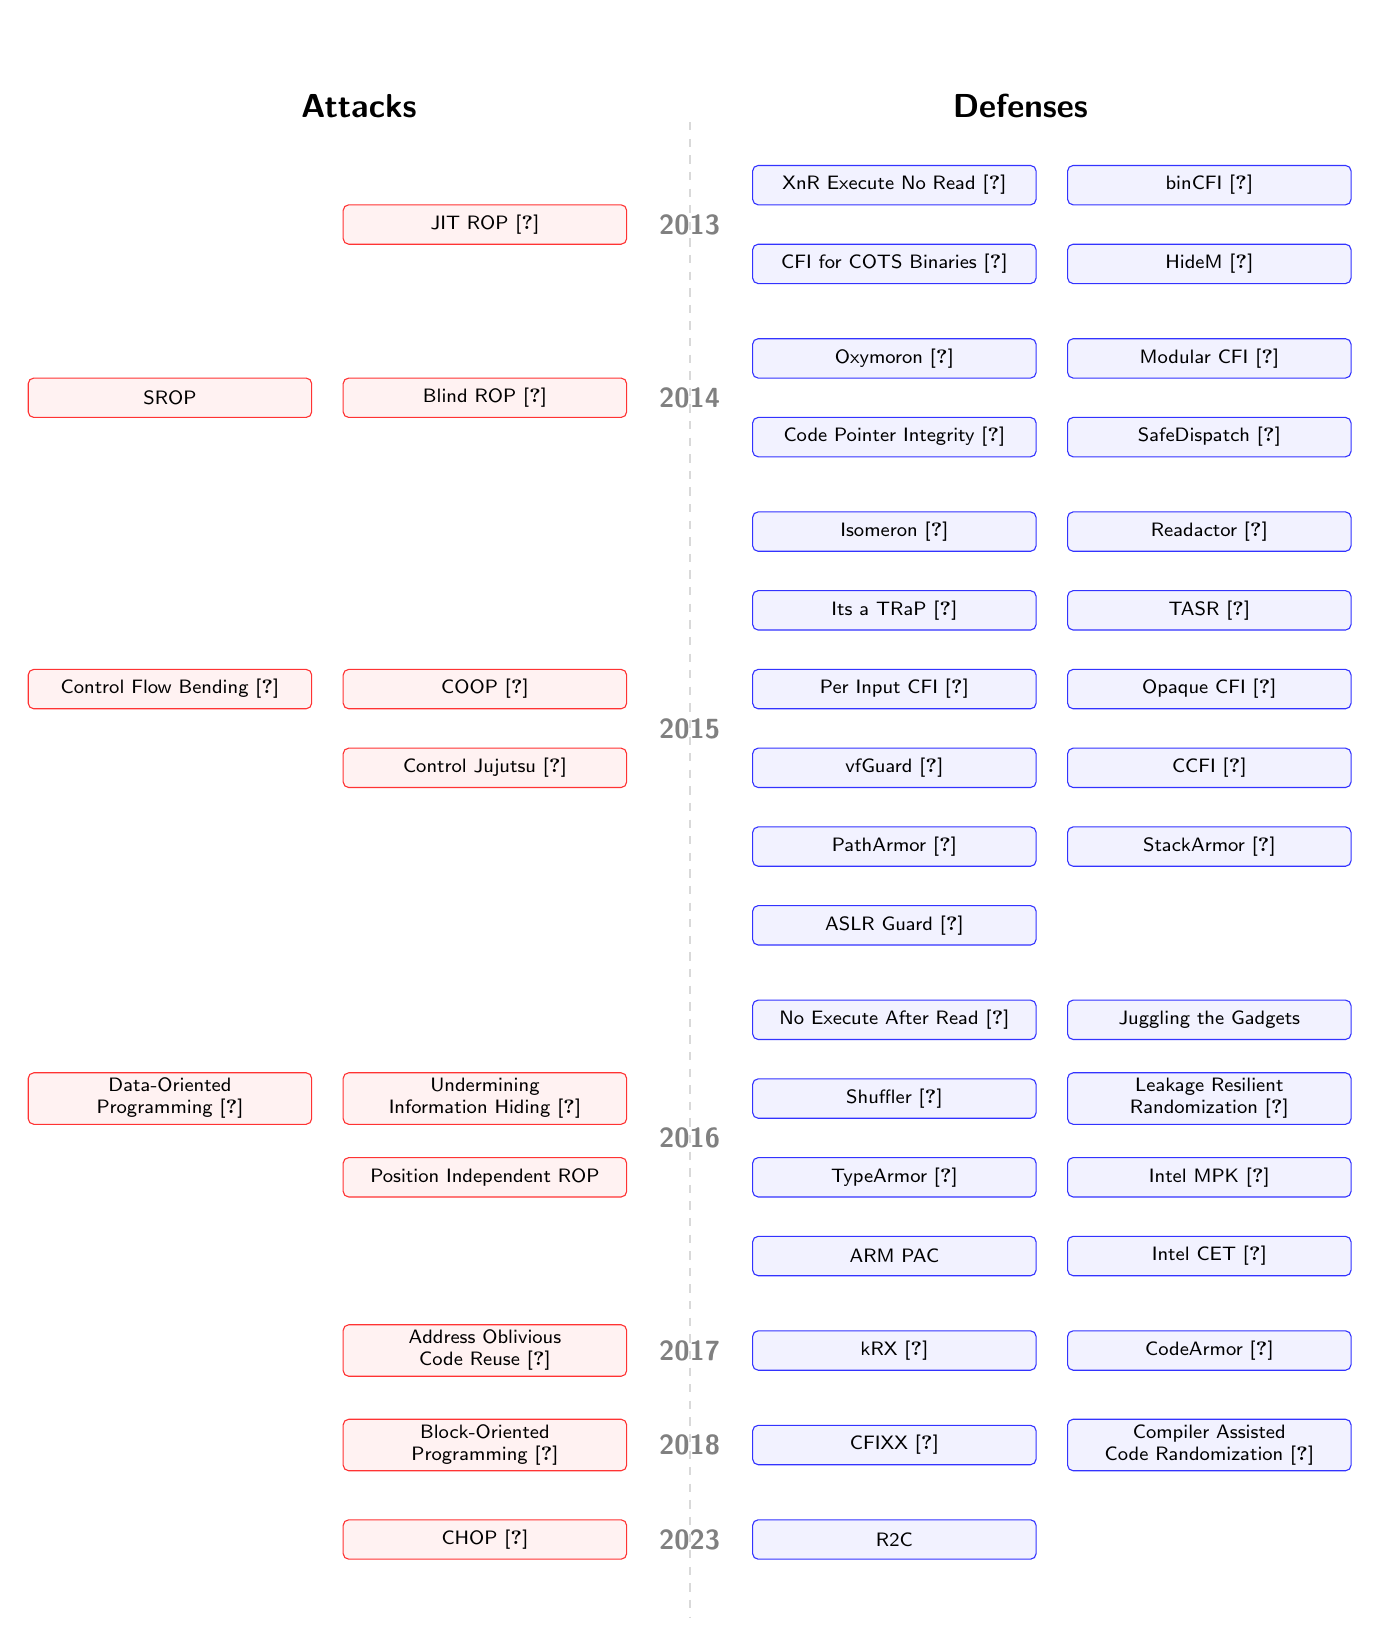
\begin{tikzpicture}[year node/.style={font=\bfseries\sffamily\color{gray}, align=center, inner sep=2pt},attack node/.style={draw=red!80, fill=red!5, rounded corners=2pt, font=\scriptsize\sffamily, align=center, minimum width=3.60cm, minimum height=0.5cm, inner sep=2pt, text width=3.40cm, execute at begin node=\setlength{\emergencystretch}{0pt}\tolerance 200\hyphenpenalty 10000\exhyphenpenalty 10000},defense node/.style={draw=blue!80, fill=blue!5, rounded corners=2pt, font=\scriptsize\sffamily, align=center, minimum width=3.60cm, minimum height=0.5cm, inner sep=2pt, text width=3.40cm, execute at begin node=\setlength{\emergencystretch}{0pt}\tolerance 200\hyphenpenalty 10000\exhyphenpenalty 10000},spine/.style={thick, gray!30, dashed}]%
\node[font=\large\bfseries\sffamily] at (-4.2,1.0) {Attacks};%
\node[font=\large\bfseries\sffamily] at (4.2,1.0) {Defenses};%
  % Year 2013%
\node[year node] at (0.0,-0.5) {2013};%
\node[attack node] at (-2.6,-0.5) {JIT ROP \allowbreak\cite{Snow2013}};%
\node[defense node] at (2.6,0.0) {XnR Execute No Read \allowbreak\cite{Backes2013}};%
\node[defense node] at (6.6,0.0) {binCFI \allowbreak\cite{zhang2013}};%
\node[defense node] at (2.6,-1.0) {CFI for COTS Binaries \allowbreak\cite{zhang2013}};%
\node[defense node] at (6.6,-1.0) {HideM \allowbreak\cite{Goktas2016b}};%
  % Year 2014%
\node[year node] at (0.0,-2.7) {2014};%
\node[attack node] at (-2.6,-2.7) {Blind ROP \allowbreak\cite{Bittau2014a}};%
\node[attack node] at (-6.6,-2.7) {SROP};%
\node[defense node] at (2.6,-2.2) {Oxymoron \allowbreak\cite{Backes2014f}};%
\node[defense node] at (6.6,-2.2) {Modular CFI \allowbreak\cite{niu2014a}};%
\node[defense node] at (2.6,-3.2) {Code Pointer Integrity \allowbreak\cite{Kuznetsov2014}};%
\node[defense node] at (6.6,-3.2) {SafeDispatch \allowbreak\cite{jang2014}};%
  % Year 2015%
\node[year node] at (0.0,-6.9) {2015};%
\node[attack node] at (-2.6,-6.4) {COOP \allowbreak\cite{Schuster2015a}};%
\node[attack node] at (-6.6,-6.4) {Control Flow Bending \allowbreak\cite{Carlini2015a}};%
\node[attack node] at (-2.6,-7.4) {Control Jujutsu \allowbreak\cite{Evans2015a}};%
\node[defense node] at (2.6,-4.4) {Isomeron \allowbreak\cite{Davi2015}};%
\node[defense node] at (6.6,-4.4) {Readactor \allowbreak\cite{Crane2015}};%
\node[defense node] at (2.6,-5.4) {Its a TRaP \allowbreak\cite{Crane2015b}};%
\node[defense node] at (6.6,-5.4) {TASR \allowbreak\cite{bigelow2015}};%
\node[defense node] at (2.6,-6.4) {Per Input CFI \allowbreak\cite{Niu2015}};%
\node[defense node] at (6.6,-6.4) {Opaque CFI \allowbreak\cite{Mohan2015}};%
\node[defense node] at (2.6,-7.4) {vfGuard \allowbreak\cite{Prakash2015}};%
\node[defense node] at (6.6,-7.4) {CCFI \allowbreak\cite{Mashtizadeh2015}};%
\node[defense node] at (2.6,-8.4) {PathArmor \allowbreak\cite{Goktas2016b}};%
\node[defense node] at (6.6,-8.4) {StackArmor \allowbreak\cite{Chen2015c}};%
\node[defense node] at (2.6,-9.4) {ASLR Guard \allowbreak\cite{Lu2015}};%
  % Year 2016%
\node[year node] at (0.0,-12.1) {2016};%
\node[attack node] at (-2.6,-11.6) {Undermining\\ Information Hiding \allowbreak\cite{Goktas2016}};%
\node[attack node] at (-6.6,-11.6) {Data{-}Oriented\\ Programming \allowbreak\cite{Hu2016}};%
\node[attack node] at (-2.6,-12.6) {Position Independent ROP};%
\node[defense node] at (2.6,-10.6) {No Execute After Read \allowbreak\cite{Werner2016}};%
\node[defense node] at (6.6,-10.6) {Juggling the Gadgets};%
\node[defense node] at (2.6,-11.6) {Shuffler \allowbreak\cite{WilliamsKing2016}};%
\node[defense node] at (6.6,-11.6) {Leakage Resilient\\ Randomization \allowbreak\cite{Braden2016}};%
\node[defense node] at (2.6,-12.6) {TypeArmor \allowbreak\cite{VanderVeen2015b}};%
\node[defense node] at (6.6,-12.6) {Intel MPK \allowbreak\cite{Wahbe1993}};%
\node[defense node] at (2.6,-13.6) {ARM PAC};%
\node[defense node] at (6.6,-13.6) {Intel CET \allowbreak\cite{IntelCET}};%
  % Year 2017%
\node[year node] at (0.0,-14.8) {2017};%
\node[attack node] at (-2.6,-14.8) {Address Oblivious\\ Code Reuse \allowbreak\cite{Rudd2017}};%
\node[defense node] at (2.6,-14.8) {kRX \allowbreak\cite{Pomonis2019}};%
\node[defense node] at (6.6,-14.8) {CodeArmor \allowbreak\cite{Chen2017a}};%
  % Year 2018%
\node[year node] at (0.0,-16.0) {2018};%
\node[attack node] at (-2.6,-16.0) {Block{-}Oriented\\ Programming \allowbreak\cite{Ispoglou2018}};%
\node[defense node] at (2.6,-16.0) {CFIXX \allowbreak\cite{Burow2018CFIXX}};%
\node[defense node] at (6.6,-16.0) {Compiler Assisted\\ Code Randomization \allowbreak\cite{Koo2018}};%
  % Year 2023%
\node[year node] at (0.0,-17.2) {2023};%
\node[attack node] at (-2.6,-17.2) {CHOP \allowbreak\cite{duta2023}};%
\node[defense node] at (2.6,-17.2) {R2C};%
\path[spine,draw] (0.0,0.8) -- (0.0,-18.2);%
\path[use as bounding box] (-8.40,-18.20) rectangle (8.40,2.00);%
\end{tikzpicture}
}%
    }
    \caption{Epoch timeline for dynamic attacks, semantic bypasses, and corresponding defenses (2013--present).}
    \label{fig:coevolution-epoch-dynamic-semantic}
\end{figure}
\section{Dynamic Attacks and Semantic Bypasses (2013--Present)}
\label{sec:epoch-dynamic-semantic}
The third epoch (2013--present) was driven by the realization that \emph{static} defenses cannot withstand \emph{dynamic} attacks.

In \citeyear{Snow2013} an attack called \gls{JITROP} showed that invalidating static a priori knowledge alone is insufficient.
\gls{JITROP} learns gadget locations by analyzing readable pointers into the code section.
In a second step, \gls{JITROP} uses this target-specific information to build a \gls{ROP} attack just in time, tailored to the target process memory layout.
A similar attack, called \gls{BROP}, exploits the behavior of certain server software to automatically respawn upon a crash~\cite{Bittau2014a}.
\gls{BROP} probes for valid gadget addresses by trying different addresses with brute force.

An attack called \gls{PIROP} showed that randomization that is too coarse-grained leaves randomized programs susceptible to partial address corruptions.
\gls{PIROP} exploits the fact that the relative distances between code units (\eg gadgets) below the randomization granularity remain constant.

As a response to \gls{JITROP} and \gls{BROP}, researchers upgraded their defenses to provide \emph{leakage-resilience}.
A key component in these defenses is to protect the randomized code with execute-only memory, thereby preventing an attacker from leaking a process' code section.
Early systems like \propername{XnR}~\cite{Backes2013} and \propername{HideM}~\cite{Giontaa2015} pioneered this approach by emulating execute-only pages in software or using split-TLB architectures.
\propername{Oxymoron} combined fine-grained randomization with execute-only memory while preserving code sharing between processes~\cite{Backes2014f}, and systems like \propername{\krx} extended these protections to the kernel~\cite{Pomonis2019}.
Execute-only memory comes in different variants, based on hardware support~\cite{Crane2015,luo2025}, with destructive code reads~\cite{Tang2015,Werner2016} or with compartmentalization~\cite{Braden2016}.
\propername{Readactor} combines fine-grained randomization with execute-only memory and \emph{booby traps}~\cite{Crane2015}.
Booby traps penalize an attacker for failed attack attempts by giving a clear signal of an ongoing attack~\cite{Crane2013,Crane2015b}.
Such a signal allows the attacked program to take counter-measures, such as preventing restarts or even retaliative action.
Taking a different approach, \propername{Isomeron} randomized the execution path rather than just the code layout by switching between diversified program variants at runtime~\cite{Davi2015}.

An alternative response to \gls{JITROP} is \emph{continuous re-randomization}.
\propername{Shuffler}, for example, re-randomizes the code layout at short intervals (50\,ms), introducing a tight deadline for disclosure~\cite{WilliamsKing2016}.
Similarly, \propername{TASR} rerandomizes at regular intervals, but instead of using a translation table, updates pointers in place~\cite{bigelow2015}.

Unable to disclose the code layout directly, a more sophisticated version of \gls{JITROP}---\emph{indirect} \gls{JITROP}---demonstrated the feasibility of inferring gadget locations from code pointers found on the stack~\cite{Davi2015,Crane2015}, which is commonly referred to as \emph{indirect information disclosure}.
In response to indirect information disclosure, \citeauthor{Crane2015} proposed \gls{CPH}~\cite{Crane2015}.
\gls{CPH} prevents disclosure by redirecting code pointers through a randomized trampoline table, located in execute-only memory.
However, \glsfirst{AOCR} demonstrated that attacks are still possible, even in the presence of \gls{CPH} or similar protection schemes~\cite{Rudd2017}.
Even without concrete information about gadgets, \gls{CPH} function pointers can be called using \emph{whole-function reuse}.
Thus, \gls{AOCR} directly challenges the \enquote{leakage resilience} postulated by Readactor.
Since the \gls{AOCR} attack is the main motivation for the defense presented in \cref{ch:r2c}, we will discuss its assumptions and principles in more detail in \cref{r2c:s:aocr}.

Just as static randomization failed against dynamic inspection, early implementations of \gls{CFI} were challenged by the inherent imprecision of static analysis and heuristics.
Because determining a precise \gls{CFG} is often undecidable, most \gls{CFI} solutions rely on an overapproximation of valid targets to avoid false positives.
This overapproximation gives attackers sufficient maneuverability to construct malicious execution paths that adhere to the previously determined allowed edges, as demonstrated by a series of attacks on \gls{CFI}~\cite{carlini2014,Carlini2015,Evans2015a,conti2015,Goktas2016b}.
An evaluation of \gls{CFI} implementations from \citeyear{li2020} shows that these issues are not merely theoretical and that some \gls{CFI} implementations even \emph{expand} the attack surface~\cite{li2020}.
Similarly, \citetitle{biondo2018} shows that implementation tradeoffs for performance can have unexpected consequences~\cite{biondo2018}.
Another related issue are semantic bypasses that target areas not covered by a \gls{CFI} solution.
For example, early \gls{CFI} defenses failed to take into account the semantics of dynamic dispatch in languages like \cpp, enabling attacks such as \gls{COOP}~\cite{Schuster2015a}.
\gls{COOP} uses virtual function calls to perform malicious computations, but from the perspective of a \cpp-oblivious \gls{CFI} \gls{COOP} stays within the legitimate \gls{CFG}.
\begin{listing}[t]
\begin{minted}{C++}
// The "Main Loop" Gadget (in existing code)
void dispatch(std::vector<Object*> &objs) {
    for (Object* obj : objs) {
        // Attacker controls 'obj' -> vtable
        obj->virtualFunc(); 
    }
}
\end{minted}
\caption{Example of a \gls{COOP} \enquote{Main Loop} gadget. An attacker can chain virtual calls by injecting a list of counterfeit objects.}
\label{lst:coop-gadget}
\end{listing}
In response, researchers have proposed \gls{CFI} solutions specialized for object-oriented languages~\cite{Gawlik2014,Zhang2015,Prakash2015,wang2018a,jang2014}.
\propername{CFIXX}, for instance, enforces strict object-type integrity on virtual calls to prevent COOP-style attacks~\cite{Burow2018CFIXX}.
Another semantic bypass called \gls{CHOP} focuses on stack unwinding and exception handlers~\cite{duta2023}.

To mitigate the shortcomings of static analysis, researchers have proposed further refinements of \gls{CFI}.
For example, \propername{OCFI} combines \gls{CFI} with code-layout randomization~\cite{Mohan2015}.
\propername{OCFI} uses the (now deprecated) MPX CPU extension to efficiently check targets against address ranges.
\propername{TypeArmor} addresses the problem of reconstructing the \gls{CFG} for binaries by considering function signatures as well~\cite{VanderVeen2015b}.
By instrumenting the program with dynamic binary instrumentation, \propername{TypeArmor} enforces conservatively determined lower and upper bounds on the number of function arguments.
\textpi{}CFI extends the traditional \enquote{code only} view of \gls{CFI} by taking concrete inputs into account~\cite{Niu2015}.
\propername{PathArmor} extends \gls{CFI} with context sensitivity by validating not only single call targets, but sequences of calls with the Intel \propername{Last Branch Register}.
\propername{OS-CFI} restricts valid call targets by taking the pointer origin into account, \eg the address-taken location of C function pointers~\cite{khandaker2019}.
\propername{CFI-LB} augments the statically determined \gls{CFG} with runtime context at the call site, such as a chain of return addresses on the stack~\cite{khandaker2019a}.
The technique behind \propername{CFI-LB} bears similarities with a concept related to fuzzer code coverage, which we will discuss in a later chapter (see \cref{psp:sec:motivation}).
Another challenge in \gls{CFG} construction is that it requires a holistic view of the entire program.
Modular control-flow integrity addresses this limitation by enabling the linkage of independently instrumented program modules~\cite{niu2014}.
Unfortunately, even precise \gls{CFG} construction cannot prevent attacks that stay entirely on legitimate control-flow paths.
\glsfirst{BOP} demonstrated that sufficiently large programs contain enough valid execution paths to construct malicious Turing-complete logic using only whole basic blocks~\cite{Ispoglou2018}.

Function returns (backward-edge control-flow transfers) are also challenging to restrict with static analysis, which is why most \gls{CFI} defenses use a different technique for returns.
The most robust form of backward-edge \gls{CFI} are shadow stacks~\cite{Burow2018a}.
A shadow stack is a separate stack in memory that holds copies of the return addresses on the regular stack.
Upon return, \gls{CFI} compares the return address on the regular stack with the return address on the shadow stack.
The motivation behind this separation is to isolate sensitive control-flow information (return addresses) from other data such as buffers.
Similar to the forward-edge case, shadow stacks must take into account semantic subtleties such as non-linear control-flow caused by C-style \code{setjmp} or \cpp exceptions.
When a \cpp function, for example, throws an exception, \cpp's stack-unwinding machinery unwinds the stack to the stack frame of a catching function (if any).

Researchers also attempted to generalize the separation of control-flow data by separating \enquote{safe} from \enquote{unsafe} data.
Techniques like \propername{StackArmor}~\cite{Chen2015c} and \gls{CPI}~\cite{Kuznetsov2014} follow this approach.
\gls{CPI}, for example, separates sensitive data like control-flow data and pointers from \eg potentially overflowing buffers.
\propername{Dataguard} later refined the policies deciding which stack objects should be separated~\cite{huang2022a}.
However, the security of this separation approach critically hinges on the protection of the isolated data against corruption and disclosure.
An initial attempt at protecting such a sensitive area in a performance-friendly way was hiding it in the vast address space of 64-bit systems.
This technique of hiding a safe area by randomizing its base address is known as \emph{information hiding}.
\propername{ASLRGuard}, for example, relies on information hiding to protect its \propername{AG-Stack}, a shadow stack implementation that includes indirect information disclosure in its threat model~\cite{Lu2015}.
Several attacks illustrate the limitations of information hiding~\cite{Goktas2016,Evans2015,Oikonomopoulos2016a}.
Even without pointer leaks, information hiding is susceptible to leakage.
By using memory allocation side-channels, attackers can disclose the safe area location.
A technique called stack spraying, for example, successfully reveals the hidden stack of code-pointer integrity~\cite{Kuznetsov2014}.
\propername{SafeHidden} attempted to harden information hiding against probing attacks by dynamically re-randomizing the safe area upon detecting suspicious memory access patterns~\cite{wang2019a}.
A more robust way to protect the sensitive area for shadow stacks is to rely on hardware features such as Intel CET or Intel MPK.
CET implements shadow stacks in hardware, whereas MPK allows the protection of arbitrary memory regions with secret keys.

\gls{CCFI} chose a different approach to enforce the \gls{CFI} policy~\cite{Mashtizadeh2015}.
Instead of instrumenting the program to check control-flow transfers against a statically computed \gls{CFG}, \gls{CCFI} cryptographically encrypts control-flow data with a \gls{HMAC}.
\gls{CCFI} provides strong security guarantees, but \gls{CCFI} incurs a significant performance overhead (up to 2.5x) and requires 12 vector registers for the cryptographic key.
The \gls{CCFI} approach was later implemented in hardware in the form of ARM's \gls{PAC}.
While \gls{CCFI} chose to outline \gls{HMAC}s into a separate table to deal with values greater than 64 bits, \gls{PAC} reuses up to 31 bits of a pointer's address upper bits to store the \gls{HMAC}.
This inlining also means, however, that the security provided by \gls{PAC} is limited by the available bits in a memory address.
This limitation makes \gls{PAC} vulnerable to cryptographic attacks, in particular offline attacks~\cite{li2022}.


To address the prohibitive overhead of full memory safety, researchers explored ways to trade precision for performance.
Techniques like \propername{Low-Fat Pointers}~\cite{kwon2013} and \propername{Delta Pointers}~\cite{kroes2017,Kroes2018} optimized metadata checks to reduce the cost of spatial safety.
Other approaches abandoned spatial enforcement entirely to focus solely on temporal safety, which can often be enforced more efficiently~\cite{dang2017a,vanderkouwe2017,lee2015}.
Despite these optimizations, software-based memory safety typically still incurs overheads that hinder widespread adoption in production systems.

\section{Transient Execution Attacks (2018--Present)}
\label{sec:epoch-transient}
In 2018, the disclosure of \propername{Spectre} and \propername{Meltdown} marked a paradigm shift in system security.
These \emph{transient execution attacks} exploit microarchitectural side-channels to leak data across protection boundaries, fundamentally challenging the assumption that architectural isolation implies security.
This discovery drew significant attention away from classical \glspl{CRA}, with researchers trying to understand and mitigate this new class of threats.
While \glspl{TEA} represent a critical threat to data confidentiality, they are not \glspl{CRA} in the traditional sense; they do not typically aim to hijack control flow to execute arbitrary code, but rather to leak information.
However, as demonstrated by \gls{JITROP} and \gls{AOCR}, information leakage is often the precursor to a successful control-flow hijack.
Despite the shift in focus towards microarchitectural defenses, the architectural vulnerabilities allowing for \gls{ROP}, \gls{COP}, and data-oriented attacks remain a critical threat.
As the \gls{AOCR} attack demonstrates, even with modern mitigations, the coupling of code and data remains a critical weakness that attackers can exploit without needing to trigger transient execution.

\section{Summary}

This chapter has traced decades of co-evolution between code-reuse attacks and defenses.
Each epoch reveals a recurring pattern: a new defense closes one attack vector, only to be circumvented by attackers exploiting a different assumption.
Code injection was stopped by \gls{DEP}, \gls{ROP} prompted both \gls{CFI} research and fine-grained randomization, and advanced attacks like \gls{COOP} and \gls{JITROP} exposed gaps in existing \gls{CFI} and randomization techniques.

While the defense categories examined in this chapter target various stages of the attack lifecycle, a holistic solution remains elusive.
Memory-safety enforcement thwarts corruption at the point of origin, yet the performance costs of achieving exhaustive spatial and temporal safety are often prohibitive.
\gls{CFI} acknowledges the likely presence of corruption but is constrained by the inherent imprecision of static analysis and gaps in semantic coverage.
Leakage-resilient randomization, while complicating attacker reconnaissance, still fails to eliminate all inference-based exploitation vectors.
In the following chapter we address a critical weakness in randomization-based defenses: the predictability of observable data that enables inference-based exploitation.

\chapter{Plugging Information Leaks With Mimicry}\label{ch:r2c}
\section{Motivation}

The previous chapter traced the arms race between code-reuse attacks and defenses.
A recurring theme in this history is that each new defense closes one avenue of attack, only for attackers to find another.
Leakage-resilient code randomization, for example, effectively prevents direct code disclosure, but as \gls{AOCR} demonstrated, predictable \emph{data} layouts---particularly on the stack---still leak enough information to mount successful attacks.

This observation motivates \rtwoc: a defense that extends the principle of randomization from code to observable data.
The key insight is that the compiler possesses precise knowledge of stack frame geometry, including the positions of return addresses, spilled registers, and local variables.
By leveraging this knowledge, the compiler can transform stack layouts to disguise sensitive pointers among indistinguishable decoys---a technique we call \emph{mimicry}.

\begin{figure}[t]
    \centering
    \includeDrawioFigure{figures/r2c/overview}{
        \draw (PointA) node {\circledtikz{\code{\footnotesize A}}};
        \draw (PointB) node {\circledtikz{\code{\footnotesize B}}};
        \draw (PointC) node {\circledtikz{\code{\footnotesize C}}};
        \draw (Compare1) node {\(\LARGE\not\equiv\)};
        \draw (Compare5) node {\(\LARGE\not\equiv\)};
        \draw (Compare2) node {\(\LARGE\equiv\)};
        \draw (Compare6) node {\(\LARGE\not\equiv\)};
        \draw (Compare3) node {\(\LARGE\equiv\)};
        \draw (Compare7) node {\(\LARGE\threeapprox\)};
        \draw (Compare4) node {\(\LARGE\equiv\)};
        \draw (Compare8) node {\(\LARGE\not\equiv\)};
    }

    \captionsetup{margin={0pt,0.3cm},oneside}
    \caption{Prior systems primarily diversify code, leaving the layout of observable data predictable (left vs middle, see \cref{s:aocr}).
    \rtwoc (right) diversifies code and observable data.}
    \vspace*{-1em}
    \label{r2c:fig:overview-unprotected-vs-protected}
\end{figure}
\section{Threat Model and Assumptions}\label{r2c:s:threat-model}

Our threat model assumes that the attacker has access to a memory corruption vulnerability that enables control-flow hijacking.
In particular, we assume that the program contains gadgets for a ROP attack as well as suitable functions for a whole-function reuse attack.
In addition, we assume that the attacker can deterministically leak stack frames (e.g., with the help of Malicious Thread Blocking)~\cite{Rudd2017}.

% \subsection{Assumptions}
Our defense integrates with existing defenses.
We assume, specifically, that the data section is protected against code injection (\eg \wox or DEP)~\cite{DEP} and the text section with some form of execute-only memory.
Due to compatibility problems with \propername{xom-switch}, we could not evaluate the impact of execute-only memory in combination with \rtwoc{}.
However, the overhead introduced by execute-only hardware solutions is generally negligible~\cite{Zhang2018}.
% Other defenses are optional to, but compatible with, Readactor.

% We discuss the mutually beneficial aspects of  \rtwoc with other defenses in (see \cref{s:discussion}).
Our implementation focuses on protecting against information disclosure through the stack or the data section.
We do not consider other types of information leaks such as side-channels~\cite{Kim2014,Lipp2018,Kocher2019}.
Note that using side channels to uncloak EPT-based execute-only memory does not work~\cite{Goktas2020}.
Side channels could, however, be used to infer heap information.

%%% Local Variables:
%%% mode: latex
%%% TeX-master: "../eurosys22"
%%% End:

\section{The Design of \rtwoc}\label{r2c:s:design}

\begin{figure*}[t]
    \centering
    \begin{subfigure}[t]{0.6\linewidth}
        \figuretitle{Unprotected stack}
        \resizebox{\linewidth}{!}{%
        %\includesvg{img/architecture-overview}
            \includegraphics[trim={0.5cm 0 12.5cm 0},clip]{figures/r2c/architecture-overview-with-heap}%
        }
        \captionsetup{margin={0pt,0.3cm},oneside}
        \caption{In an unprotected stack frame the return address is at a predictable location surrounded by known values.}
        \label{r2c:fig:overview-stack-unprotected}
    \end{subfigure}
    \hfill
    \begin{subfigure}[t]{0.6\linewidth}
        \figuretitle{Stack protected with \rtwoc{}}
        \resizebox{\linewidth}{!}{%
            \includegraphics[trim={12.5cm 0 0.5cm 0},clip]{figures/r2c/architecture-overview-with-heap}%
%            }
        }
        \captionsetup{margin={0.3cm,0pt},oneside}
        \caption{\rtwoc inserts Booby-Trapped Return Addresses to conceal the return address and thus protect it from disclosure.}
        \label{r2c:fig:overview-stack-protected}
    \end{subfigure}
    \caption{The stack layout of an unprotected stack (\emph{top}) and a stack protected by \rtwoc (\emph{bottom}). We assume the System V ABI on the x86\_64 platform.}
    \label{r2c:fig:overview-stack}
\end{figure*}

%    We observe that the predictable location of return addresses makes them vulnerable to disclosure.
%    Previous stack frame diversification techniques have focused on permuting stack objects and on inserting random paddings between the stack frames.
%    These techniques harden against the profiling of function pointers in \gls{AOCR}.
%    Return addresses, however, keep their relative position to other stack objects and remain vulnerable to disclosure.

%    maybe explain why hiding the return address with IH is a bad idea
\rtwoc is a leakage-resilient diversity defense against advanced code-reuse attacks.
As such, \rtwoc's main objective is to prevent information leakage that could help an attacker to undermine the effects of randomization.
As a first step, and under the protection of execute-only memory, \rtwoc randomizes the order of functions in the text section to thwart ROP and JIT-ROP attacks.
\rtwoc{} further aims to remove the building blocks of sophisticated code-reuse attacks such as indirect JIT-ROP and \gls{AOCR}:
\begin{enumerate}
[label={(\roman*)}]
    \item a predictable layout of global variables as a means to manipulate function arguments in a whole-function reuse attack;
    \item the stack as a source for code and heap pointer leaks.
\end{enumerate}
Similar to Readactor\plusplus, \rtwoc protects global variables by randomizing their order and by inserting random padding~\cite{Crane2015b}.
Protecting the stack against leakage is more challenging.
Stack data necessarily has to remain readable, which poses the question of how to protect information in plain sight.

%%% 20210507/0950/sbr/ccs2021.tex#595:
%%% reordered paragraphs to: highlight overall design, going deep into challenges, and closing how our overall design addresses these challenges!

To illustrate the challenges of protecting the stack, consider the unprotected stack frame in \cref{r2c:fig:overview-stack-unprotected}.
\cref{r2c:fig:overview-stack-unprotected} shows the stack frame of a function when called \emph{from} function \code{F} on the x86\_64 platform with the System V ABI calling convention.
When locating pointers on the stack, an attacker can tap two sources of information.
First, an attacker can leverage the predictable location of pointers relative to other stack objects.
If the adversary has information pertaining to some of these stack objects (\eg the value \code{0xaaaa} of a local variable \code{A} in function \code{F}), they can use this information as an anchor to locate the pointer.
For example, in \cref{r2c:fig:overview-stack-unprotected} the return address is one machine word below function variable \code{A} and adjacent to the spilled base pointer (\texttt{rbp}).
Second, an attacker can locate pointers based on their value ranges.
The heap pointer in \cref{r2c:fig:overview-stack-unprotected}, for example, has a different address range than code pointers or the spilled base pointer.
If both of these methods fail, an attacker can still resort to guessing.
Under specific circumstances, such brute-force attacks are a reasonable option; some servers restart crashed worker processes without reloading their binary code images (\eg nginx, Apache, OpenSSH)~\cite{Bittau2014a}.

The core idea behind \rtwoc's techniques is \emph{mimicry}: deliberately disguising sensitive information by surrounding it with similar-looking data, so that the real object cannot be distinguished using either spatial or semantic cues.
In practice, this means creating decoys that match the appearance and behavioral characteristics of the protected object.
For example, addresses that have the same alignment, size, and value-range properties as genuine return or heap pointers, and that are positioned unpredictably relative to other stack objects.
By making decoys and real pointers statistically and structurally similar, mimicry removes the usual anchors an attacker uses (predictable offsets, value ranges, and layout patterns) and forces an adversary to guess.
\rtwoc further penalizes guessing attempts with booby traps, which afford an attacker at most one incorrect guess.
Mimicry therefore raises the cost and risk of disclosure attacks while preserving normal program semantics for non-adversarial execution.

We instantiate this principle for return addresses and for heap pointers as follows:
\begin{enumerate}
[label=(\roman*)]
%    \vspace*{-0.5cm}
    \item So-called \emph{booby-trapped return addresses}, or \glspl{BTRA} for short, randomize the precise position of a return address in a stack frame.
    By inserting \glspl{BTRA}, \rtwoc changes the relative position of the return address to other stack objects.
    An attacker is, therefore, no longer able to rely on specific stack objects as anchor points to locate the return address.
    In addition, \glspl{BTRA} disguise the return address among enclosing and similar-looking values, as they are specifically chosen to look and behave exactly like benign return addresses.
    \glspl{BTRA} point to booby-trap functions randomly distributed in the text section.
    Without exact code-layout information, an adversary cannot separate \glspl{BTRA} from benign addresses.

    \item A combination of \emph{booby-trapped data pointers}, or \glspl{heapbt} for short, and stack slot randomization protects heap pointers against disclosure.
    Stack object permutation randomizes the position of heap pointers relative to other stack objects.
    The insertion of \glspl{heapbt} misleads \gls{AOCR}'s statistical analysis based on pointer value ranges.
    As \glspl{heapbt} point into the heap like benign heap pointers, both share the same value range.
    To protect against brute force attacks, \glspl{heapbt} point into guard pages.
    Dereferencing a \gls{heapbt} causes an immediate fault, giving defenders a way to respond to an ongoing attack.

\end{enumerate}

The following subsections give an in-detail presentation of the relevant design decisions and requirements.
First, we describe the details on inserting booby-trapped return addresses (see \Cref{r2c:ss:decoy-mimicry}).
Second, we explain how \glspl{heapbt} thwart the localization of heap pointers (see \Cref{r2c:ss:heap-boobytraps}).
Third, we illustrate how additional code randomization strengthens the protection afforded by \glspl{BTRA} and \glspl{heapbt} (see \Cref{r2c:ss:strengthening}).
Both \glspl{BTRA} and \glspl{heapbt} leverage the principle of mimicry, \ie disguising sensitive objects among covert booby traps.
In \cref{r2c:ss:speculative-booby-traps} we discuss an extension of this principle into the speculative domain.

\subsection{Booby-Trapped Return Addresses}\label{r2c:ss:decoy-mimicry}
An indispensable prerequisite for effective \glspl{BTRA} is that they must be virtually indistinguishable from actual, benign return addresses.
For \glspl{BTRA} to masquerade as return addresses, they must:
\begin{enumerate*}[label={(\roman*)}]
    \item look like return addresses;
    \item behave like return addresses;
    \item resist brute force attacks.
\end{enumerate*}

To achieve the first and the third goal, \glspl{BTRA} point to booby trap functions.
Booby trap functions are distributed randomly in the \emph{text section}, giving \glspl{BTRA} the same value range as benign return addresses.
Absent exact information about return addresses and leakage through side channels, an attacker could still apply brute-force.
\gls{BROP}, for example, demonstrates the effectiveness and feasibility of brute-force to learn the location of a \code{read} gadget~\cite{Bittau2014a}.
Booby traps provide an effective way to penalize such brute force attempts~\cite{Crane2013}.
In the context of \rtwoc, a classic \gls{BROP} attack is infeasible for two reasons:
\begin{enumerate*}[label={(\roman*)}]
    \item the booby trap functions distributed in the text section deter attempts to blindly locate gadgets with brute force;
    \item execute-only memory prevents \gls{BROP} from disclosing the text section with a found \texttt{read} gadget.
\end{enumerate*}
Likewise, brute forcing an attack with all return address candidates is improbable because all but one of the candidates lead to a booby trap function.
We discuss the combination of Blind ROP with the more powerful PIROP attack in \cref{r2c:sss:corrupting-code-pointers}.

To achieve the second goal, \glspl{BTRA} mimic the runtime behavior of return addresses.
Since return addresses are part of the control flow of a program, they show a distinct observable runtime behavior.
Recall the following properties of return addresses and call sites, which must also hold for booby-trapped return addresses:
\begin{enumerate}[label=(\Alph*)]
    \item \label{itm:raprop1} A return address occurs exactly once in the stack frame;
    \item \label{itm:raprop2} Multiple invocations of the same call site have the same return address;
    \item \label{itm:raprop3} Different call sites have different return addresses.
\end{enumerate}
% \glspl{BTRA} must have these properties as well.
Violating any of these properties might allow an attacker to learn the actual return address.
%%% 20201118/1654/sbr/sp2021-urad.tex#519: parallel sentence construction...
We take the following precautions to preserve the properties.
To preserve property~\ref{itm:raprop1}, \rtwoc{} ensures that each call site uses the same booby-trapped return address just once.
To preserve property~\ref{itm:raprop2}, \rtwoc{} does \emph{not} change the set of \glspl{BTRA} for a call site at run-time.
This decision represents a rare case, where \emph{more} dynamism is \emph{less} effective.
Consider a single call site with dynamically changing \glspl{BTRA}: just two observations suffice to identify the return address, as it is the only pointer remaining identical.
To preserve property~\ref{itm:raprop3},  \rtwoc{} inserts a randomly chosen set of \glspl{BTRA} at each \emph{call-site}.
If, instead, one were to insert them in the \emph{callee}, multiple call sites would have the identical set of \glspl{BTRA}, with only one difference: the return address.

For this very reason---preserving property~\ref{itm:raprop3}---\rtwoc{} also avoids reusing booby-trapped return addresses between different call sites as much as possible.
% \rtwoc also tries to avoid reusing \glspl{BTRA} between different call sites, as doing so would violate \cref{itm:raprop3}.
In particular, an attacker could leak multiple stack frames and look for recurring addresses to identify \glspl{BTRA}.
Due to the ensuing combinatorial explosion, avoiding the reuse of \glspl{BTRA} between call sites becomes increasingly difficult with an increasing number of call sites.
To counter this combinatorial effect, we tolerate occasional reuse and parameterize the maximum number of \glspl{BTRA}.
An attacker would have to leak two specific stack frames reusing the same \glspl{BTRA} to gain valuable information.
Such a leak is unlikely in practice because the \glspl{BTRA} are distributed randomly over the text section.

\subsection{Booby-Trapped Data Pointers}\label{r2c:ss:heap-boobytraps}
Contrary to return addresses, the runtime requirements for non-control-flow related stack objects are not as strict.
Stack objects like local variables, for example, can be permuted freely within the stack frame.
Such a reordering invalidates any a priori knowledge an attacker might have regarding the relative position of stack objects to each other.

Without the knowledge of stack object positions, an attacker can still resort to analyzing the value ranges of stack objects.
The \gls{AOCR} paper demonstrates that a statistical analysis of two pages of stack values suffices to reliably identify heap pointers.
Due to the large address space of x64 systems, the values of pointers occur in clusters, with heap pointers typically constituting the third-largest cluster.
To reach the heap, an attacker does not necessarily need to identify a \emph{specific} heap pointer.
Note, however, that thanks to stack slot randomization, an attacker also \emph{cannot} reliably identify a specific heap pointer.
Instead, an attacker has to pick and dereference an arbitrary pointer from the cluster of heap pointers.
\rtwoc{} uses this insight to penalize the random choice by mixing \glspl{heapbt} into the cluster of benign heap pointers.
\glspl{heapbt} point into randomly distributed guard pages on the heap, thus, sharing the same value range as benign heap pointers.
A statistical analysis will, thus, sort \glspl{heapbt} and benign heap pointers into a single cluster.
If an attacker dereferences a \gls{heapbt}, she causes a segmentation fault that can be handled by the program or a monitoring system.

\subsection{Strengthening \rtwoc Through Code Randomization}\label{r2c:ss:strengthening}
To strengthen security, \rtwoc diversifies the code layout at a subfunction granularity.
To this end, \rtwoc randomly inserts NOP instructions at call sites, traps in function prologs, and randomizes register allocation~\cite{Crane2015, Pappas2012a}.
By diversifying these function parts, two specific types of inference are impeded:
\begin{enumerate*}[label=(\roman*)]
    \item from return addresses to function addresses, and
    \item from function addresses to gadget locations.
\end{enumerate*}

The inserted NOPs at a call site change the relative offset between the return address and the calling function address.
As a result, an attacker can no longer reliably infer the function address from a leaked return address, effectively restricting the use of return addresses to \emph{gadget localization}.
Whereas for a whole-function reuse attack a \emph{single} function pointer might suffice, an attacker typically needs multiple leaked addresses to locate enough gadgets for a gadget chain.
Return addresses are protected by \glspl{BTRA} and increasing the number of required leaks increases the probability of an attacker choosing a \gls{BTRA} over the real return address.
Thus, increasing the number of required leaks increases the overall security.

The inserted traps in the prolog change the relative offset from the function start to a potential gadget location.
An attacker leaking a function pointer can, therefore, no longer reliably infer gadget locations and is restricted to \emph{whole-function reuse}.
Although in principle, a single leaked function pointer might suffice, whole-function reuse attacks have stricter requirements on the leaked function pointers (\eg corruptible default parameters).
Potential leaks are therefore less likely to meet those requirements.
%% Function pointers on the stack are also less frequent than return addresses and are also protected by stack slot randomization.
Compared with return addresses, function pointers on the stack occur less frequently and are, furthermore, protected by stack slot randomization.
% Instead of crashing the target process, booby traps can actively react to an ongoing attack.
% For example, a booby trap could prevent the restart of a crashed process, patch vulnerable code or start a honeypot process instead.




%%    \subsection{Adaptive Security}\label{r2c:ss:adaptive-security}
%%    \rtwoc provides probabilistic security against the disclosure of return addresses.
%%    Specifically, each inserted BTRA decreases the success rate of a blind guess, while increasing the necessity for more observations.
%%    At the same time, however, inserting additional BTRAs impacts the performance and code size.
%%    For that reason the number of BTRAs before and after the return address is configurable and can be tuned according to performance and security needs.
%%    There are several choices when choosing the number of BTRAs.
%%    One option is to use the same number for each call site.
%%    Another option is to randomly choose the number of BTRAs based on a configurable random trial.
%%    The performance of these variants is analyzed in \cref{s:eval}.
%%
%%    Static parameters or random selection do not take into account the different performance and security profiles of call sites.
%%    The power of adaptive security lies in the ability to control parameter selection with additional information.
%%    Programs, for example, typically spend most of their execution time in only few regions of the code, called hot regions~\cite{Pettis1990}.
%%    Adding more BTRAs to call sites in hot regions has a correspondingly bigger impact on performance than increasing BTRAs in cold regions.
%%    In \cref{r2c:ss:impl-pgo} we demonstrate how profiles can change the parameter selection based on the execution frequency of a call site.
%
%%    \fbetodo{Should we move this paragraph to discussion as future work?}
%%    Another option is to use application specific information.
%%    For instance, observe that stack frames are not equally vulnerable to information disclosure.
%%    To reliably leak a stack frame, the frame must occur in the call stack of a function blocked with Malicious Thread Blocking.
%%    Analogously, not all return addresses are equally desirable.
%%    Attackers are particularly interested in return addresses that reveal functions beneficial for an attack.
%%    Analyses uncovering these weak spots could drive the parameter selection to specifically harden the security of vulnerable call sites.

%%% Local Variables:
%%% mode: latex
%%% TeX-master: "../eurosys22"
%%% End:

\section{The \rtwoc{} Compiler}\label{r2c:s:implementation} % maximum 2-3 pages...
We implemented \rtwoc using the LLVM compiler framework~\cite{Lattner2004}.
Our modified compiler supports the compilation of a wide range of systems software for the Linux \code{x86\_64} platform (see \cref{r2c:ss:scalability}).
To support complex applications like Webkit, \rtwoc{} is fully compatible with \gls{PIC} for ASLR, stack unwinding, and exception handling.
\rtwoc combines a multitude of different diversification techniques, including function shuffling, global variable shuffling, register-allocation randomization and NOP insertion.
In addition, \rtwoc supports two new diversification techniques that we describe in more detail in the following sections.
Specifically, our compiler
\begin{enumerate*}[label=(\roman*)]
    \item instruments call sites with booby-trapped return addresses (see \cref{r2c:ss:impl-btras});
    \item instruments functions to insert \glspl{heapbt}, which thwart the statistical analysis of pointers on the stack (see \cref{r2c:ss:impl-heap-boobytraps}).
\end{enumerate*}

\subsection{BTRAs: Booby-Trapped Return Addresses}\label{r2c:ss:impl-btras}

\newsavebox{\btrasetup}
\begin{lrbox}{\btrasetup}
    \begin{lstlisting}[style=asmcode,style=coloredrads]
push BTRA1
push BTRA2
push RA
push BTRA3 |\circledtikz{1}|
add %rsp, 0x10 |\circledtikz{2}|
call F|\tikzmark{T-Call-Setup}| |\circledtikz{3}|
add %rsp,0x10|\tikzmark{T-Add-Cleanup}| |\circleddashedtikz{7}|
    \end{lstlisting}
\end{lrbox}

\newsavebox{\btrateardown}
\begin{lrbox}{\btrateardown}
    \begin{lstlisting}[style=asmcode]
|\tikzmark{T-Function}|<F>:
sub %rsp,0x8 |\circledtikz{4}|

    |\raisebox{-1pt}[0pt][0pt]{$\vdots$}|

add %rsp,0x8 |\circleddashedtikz{5}|
|\tikzmark{T-Ret-Setup}|ret |\circleddashedtikz{6}|
    \end{lstlisting}
\end{lrbox}
\newlength{\btracodegap}
\setlength{\btracodegap}{6em}
\newlength{\btracodewidth}
\setlength{\btracodewidth}{\dimexpr\wd\btrasetup+\wd\btrateardown+\btracodegap\relax}

\begin{figure}[t]
    \begin{subfigure}[t]{\linewidth}
        \centering
        \begin{minipage}{\btracodewidth}
            \usebox\btrasetup\hspace{\btracodegap}\usebox\btrateardown
        \end{minipage}
        \caption{Cooperation between caller (\emph{left}) and callee (\emph{right}) to insert \glspl{BTRA}.}
        \label{r2c:fig:rad-insertion-code}
    \end{subfigure}
    \begin{tikzpicture}[overlay, remember picture]
        \draw[-Latex] ([shift={(18pt,2pt)}] pic cs:T-Call-Setup) -- +(1.6,0) |- ([shift={(-7pt,2pt)}] pic cs:T-Function);
        \draw[-Latex] ([shift={(-10pt,1pt)}] pic cs:T-Ret-Setup) -- ([shift={(18pt,2pt)}] pic cs:T-Add-Cleanup);
    \end{tikzpicture}
    \begin{subfigure}[t]{\linewidth}
        \centering
        \includeDrawioFigure[\linewidth]{figures/r2c/btra-setup}{
            \draw ([yshift=-10pt] Arrow1) node {\circledtikz{\code{1}}};
            \draw ([yshift=-10pt] Arrow2) node {\circledtikz{\code{2}}};
            \draw ([yshift=-10pt] Arrow3) node {\circledtikz{\code{3}}};
            \draw ([yshift=-10pt] Arrow4) node {\circledtikz{\code{4}}};
            \draw ([yshift=-10pt] Arrow5) node {\circleddashedtikz{\code{5}}};
            \draw ([yshift=-10pt] Arrow6) node {\circleddashedtikz{\code{6}}};
            \draw ([yshift=-10pt] Arrow7) node {\circleddashedtikz{\code{7}}};
        }
        \caption{Stack view of the booby-trapped return address setup and teardown process.}
        \label{r2c:fig:rad-insertion-stack}
    \end{subfigure}%
    \caption{Insertion and deletion of booby-trapped return addresses: Code perspective (\Cref{r2c:fig:rad-insertion-code}), and effect on the stack (\Cref{r2c:fig:rad-insertion-stack}).
    For brevity the figure uses only two \glspl{BTRA} before (\texttt{\gls{BTRA}1}) and (\texttt{\gls{BTRA}2}) and one \gls{BTRA} after (\texttt{\gls{BTRA}3}) the return address.}
    \label{r2c:fig:btra-insertion}
\end{figure}

% To this end, \rtwoc encloses return address with BTRAs.
To enclose return addresses with \glspl{BTRA}, steps \Circled{\code{1}} to \Circled{\code{4}} in \cref{r2c:fig:btra-insertion} are required.
First, the caller pushes randomly chosen \glspl{BTRA} together with the return address on the stack \Circled{\code{1}}.
Note that the position of the return address within the sequence of \glspl{BTRA} is chosen randomly at compile time.
Second, the caller positions the stack pointer above the return address \Circled{\code{2}}.
Third, the caller executes the \texttt{call} instruction \Circled{\code{3}}.
On x86, \texttt{call} instructions implicitly perform two operations:
\begin{enumerate*}[label=(\roman*)]
    \item write the return address to the current stack pointer position;
    \item transfer control to the callee.
\end{enumerate*}
Due to the prior positioning of the stack pointer, the call instruction overwrites the return address already on the stack.
Put differently, the addresses on the stack \emph{do not change} after step \Circled{\code{1}}.
Writing all the addresses to the stack at once eliminates the possibility for a race condition window during which an attacker could observe stack changes.
If, for example, only the \glspl{BTRA} were inserted before the call, the attacker could learn the return address by observing the stack right before and after the call instruction~\cite{Pomonis2017}.
While such a precise timing might seem unattainable in practice, a similar race-condition attack forced Microsoft to rethink their Return Flow Guard architecture~\cite{Bialek2018}.

The position of the return address chosen by the \emph{caller} defines how many \glspl{BTRA} \emph{precede} the return address.
The preceding \glspl{BTRA} create an offset between the return address and caller stack objects (\eg local variables in the caller).
We call the resulting offset \emph{pre-offset}.

After the control-flow transfer, the stack pointer points directly below the return address, still pointing into the \gls{BTRA} sequence.
Subsequent register spills in the callee would, therefore, overwrite \glspl{BTRA} below the return address.
To avoid overwriting the \glspl{BTRA}, in the last step the callee decreases the stack pointer by a random offset \Circled{\code{4}}.
The random offset chosen by the \emph{callee} defines the number of \glspl{BTRA} that \emph{succeed} the return address.
The succeeding \glspl{BTRA} create an offset between the return address and callee stack objects (\eg spilled registers).
This resulting offset is called a \emph{post-offset}.

After adjusting the stack pointer, the callee executes the regular function prologue.
When reaching the epilogue of the callee, the setup process is reversed as shown in \cref{r2c:fig:btra-insertion}, steps \circleddashedtikz{\code{5}} to \circleddashedtikz{\code{7}}.
First, to identify the correct return address, the callee reverts the post-offset \circleddashedtikz{\code{5}} before executing the return instruction.
Next, the return instruction pops the return address from the stack \circleddashedtikz{\code{6}} and transfers control back to the caller.
Finally, the caller reverts the pre-offset \circleddashedtikz{\code{7}}, which is required to perform stack-relative operations, such as referencing spilled local variables or function parameters.

Since the caller chooses the \emph{number} of \glspl{BTRA} to push and the \emph{pre-offset}, while the callee chooses the \emph{post-offset}, caller and callee cooperate in the setup of \glspl{BTRA}.
For direct call sites, \rtwoc bounds the number of \glspl{BTRA} after the return address at compile-time to fit into the \emph{post-offset}.
For indirect call sites, no synchronization between the caller and the callee is possible at compile time.
Instead, we tolerate that the caller potentially overwrites \glspl{BTRA} after the return address.
Per default, \rtwoc does not add \glspl{BTRA} to call sites that call unprotected code.
While adding \glspl{BTRA} would not harm functionality, unprotected callees would overwrite \emph{all} \glspl{BTRA} after the return address.
We discuss the security implications in \cref{r2c:ss:limitations-coverage}.
Our \glspl{BTRA} implementation cooperates with ThinLTO to match as many caller-callee pairs at compile time as possible.

Emitting the setup code for \glspl{BTRA} happens in a target-specific pass.
This pass is also responsible for inserting the boobytrap functions to which the \glspl{BTRA} point.
In the current implementation, a boobytrap function simply jumps to a notification routine.
A refined implementation could let the \glspl{BTRA} point to boobytrap regions \emph{within} the caller function.
Depending on the relocation model and the setup instructions, the \glspl{BTRA} are either embedded in the \code{push} instructions or read from the data section.
Since an attacker cannot predictably identify the return address among the \glspl{BTRA}, storing the addresses in the data section does not compromise security.

If the randomly chosen number of \glspl{BTRA} before the return address is odd, \rtwoc{} inserts an additional \gls{BTRA} to keep the stack aligned.
On x86-64, the stack pointer must be 16-byte aligned, as programs crash when certain instructions access a misaligned stack.

\subsubsection{Stack Arguments}\label{r2c:sss:stack-arguments}

\begin{figure}[t]
    \centering
    \begin{subfigure}[t]{0.3\linewidth}
        \centering
        \includegraphics[width=0.9\linewidth]{figures/r2c/parameter-addressing-plain}
        \caption{Without \cfs the base pointer points below the spilled base pointer.}
        \label{r2c:fig:stack-arguments}
    \end{subfigure}
    \quad
    \begin{subfigure}[t]{0.3\linewidth}
        \centering
        \includegraphics[width=0.9\linewidth]{figures/r2c/parameter-addressing-btra}
        \caption{With \cfs the caller positions the base pointer below the first stack argument.}
        \label{r2c:fig:stack-arguments-with-btras}
    \end{subfigure}
    \caption{\rtwoc{} uses \cfs{} to account for the dynamic offset introduced by \glspl{BTRA}.}
\end{figure}

The \glspl{BTRA} inserted by \rtwoc change the distance between stack objects above and below the return address.
In particular, the distance increases by the sum of pre- and post-offset.
This increased distance typically does not cause any compatibility issues because most functions do not access stack objects above their return address.
With one notable exception:
In the System V ABI a caller must pass arguments that do not fit into parameter registers on the stack, \emph{above} the return address.
Consider, for example, the stack arguments in the stack frame in \cref{r2c:fig:stack-arguments}.
The argument values \code{0x7} and \code{0x8} are located above the return address in the illustrated stack frame.
LLVM uses either the frame pointer, or the stack pointer as an anchor to access stack arguments.
Which pointer is actually used depends on the optimization level and several other factors.
Functions that need stack realignment, for example, cannot use the stack pointer for addressing stack arguments.
Without \glspl{BTRA}, the compiler determines the distance between a stack argument and the anchor statically.
With \glspl{BTRA}, however, the distance is not known at compile-time.
Although pre-offset and post-offset are chosen at compile-time, the pre-offset can be different for each call site.
As a result, the distance---i.e., the sum of pre-offset and post-offset---depends not only on the function but also its caller.


To access stack arguments despite the varying distance, we devised a method called \emph{\cfs}.
\Cfs moves the setup of the frame pointer from the function prologue to the call site.
In particular, the caller positions the frame pointer \emph{before} the varying pre-offset (see \cref{r2c:fig:stack-arguments-with-btras} for an illustration).
Thus, the distance between the frame pointer and the stack arguments can be computed statically.
In the callee we omit the frame pointer setup, and use the already prepared frame pointer to access stack arguments.

\Cfs is required for all functions using both \glspl{BTRA} and stack arguments.
As \cfs requires a frame pointer, it inhibits an optimization called frame-pointer omission.
Frame-pointer omission re-purposes the frame register as a general purpose register and addresses all stack arguments via the stack pointer instead.
We discuss the introduced performance overhead in \cref{sec:r2c:evaluation}.

\subsubsection{Optimization with AVX2}
\begin{figure}[t]
        % --- ROW 1: GRAPHICAL CONTENT ---
        % This row contains the graphics, aligned at their bottom edges.

    \begin{minipage}[b]{0.4\linewidth}
        \begin{lstlisting}[style=asmcode,style=coloredrads]
vmovdqa %ymm13,(arr) |\tikzmark{T-First-Vex-Mov}|
vmovdqu -0x20(%rsp),%ymm13
vmovdqa %ymm13,0x20(arr) |\tikzmark{T-Second-Vex-Mov}|
vmovdqu -0x40(%rsp),%ymm13
vzeroupper
sub $0x30,%rsp
call callee
        \end{lstlisting}
        \vspace{1cm}
    \end{minipage}%
    \hfill%
\begin{minipage}[b]{0.5\linewidth}
        \includeDrawioFigure[\linewidth]{figures/r2c/avx-setup}[remember picture]{
            \path
            (Point1) coordinate (A)
            ([yshift=5pt] Point2) coordinate (B)
            (A) -- (B) coordinate[pos=.5] (M1)
            coordinate (BraceTip1) at ($ (M1)!{7pt+5pt}!-90:(B) $);
            \draw[decorate,decoration={brace,mirror,amplitude=7pt,raise=5pt}] (A) -- (B);
            \path
            ([yshift=5pt] Point2) coordinate (C)
            ([yshift=5pt] Point3) coordinate (D)
            (C) -- (D) coordinate[pos=.5] (M2)
            coordinate (BraceTip2) at ($ (M2)!{7pt+5pt}!-90:(D) $);
            \draw[decorate,decoration={brace,mirror,amplitude=7pt,raise=5pt}]
            (C) -- (D);
        }
    \end{minipage}
    \begin{tikzpicture}[remember picture, overlay]
        \draw[Latex-, line width=0.7] ([yshift=3pt]pic cs:T-First-Vex-Mov) -| ($ (pic cs:T-First-Vex-Mov)!0.4!(BraceTip1) $) |- ([xshift=-3pt]BraceTip1);
        \draw[Latex-, line width=0.7] ([yshift=3pt]pic cs:T-Second-Vex-Mov) -| ($ (pic cs:T-Second-Vex-Mov)!0.4!(BraceTip2) $) |- ([xshift=-3pt]BraceTip2);
    \end{tikzpicture}

    % --- ROW 2: CAPTIONS ---
    % This row contains the captions, aligned at their top edges.
    % The \subcaption command will work inside the minipage.
    \caption{\Gls{BTRA} setup with AVX2 instructions.
    The AVX2 instructions load the \glspl{BTRA} from a call-site specific array in the data section (\code{arr}) and write them to the stack in batch.}
    \label{r2c:fig:avx2-setup}

\end{figure}
Implementing the \gls{BTRA} setup with \code{push} instructions is conceptually straightforward, but exerts significant pressure on the instruction cache.
%    During the performance evaluation we noticed a performance impact particularly on call intensive benchmarks.
%    We speculate that the large number of instructions puts pressure on the instruction cache.
To improve \rtwoc{}'s performance, we built an optimized variant that sets up the \glspl{BTRA} and the return address with AVX2 vector instructions (see \cref{r2c:fig:avx2-setup})~\cite{IntelAVX}.

Before each call site, we initialize a vector register with \glspl{BTRA} and the return address and write them to the stack.
The addresses are read from a call-site specific array in the data section, prepared at compile time.
Regarding the security of reading the addresses from the data section, the same reason as for the \gls{GOT} holds.
After the \glspl{BTRA} and the return address are written to the stack, \rtwoc{} positions the stack pointer before the return address.
The \code{vmovdqa} instructions load the addresses from the data section into an AVX2 register.

The \code{vzeroupper} instruction is needed to eliminate a penalty when switching between SSE and AVX2 instructions.
Note that zeroing the upper half of the vector registers directly before a call does not affect program correctness.
Since the affected registers are caller saved, the caller has to save and restore them before a call anyway if they are used by subsequent basic blocks.
Without \code{vzeroupper} we observed a performance impact of up to 50\%.

We discuss the overall performance improvements afforded by the AVX2 instructions in \cref{r2c:ss:perf}.

\newsavebox{\uninstrumented}
\begin{lrbox}{\uninstrumented}

    \begin{lstlisting}[style=asmcode,breaklines=false]
|\raisebox{-1pt}[0pt][0pt]{$\vdots$}|

call F|\tikzmark{T-Right-Start}|

|\raisebox{-1pt}[0pt][0pt]{$\vdots$}|
    \end{lstlisting}
\end{lrbox}

\newsavebox{\instrumented}
\begin{lrbox}{\instrumented}

    \begin{lstlisting}[style=asmcode,breaklines=false,xleftmargin=2em]
|\tikzmark{T-Before-Begin}|push BTRA1
push BTRA2
|\tikzmark{T-Before-End}|push BTRA3
push BTRA3
|\tikzmark{T-After-Begin}|push BTRA5
|\tikzmark{T-After-End}|push BTRA6
add %rsp, |$(\beta+1)*8$|
call F
add %rsp, |$\alpha*8$|

    \end{lstlisting}
\end{lrbox}
\tikzset{
    pics/numberline/.style n args={4}{
        code = { %
            \coordinate (#3) at (0,0);
            \coordinate (#4) at (0,1);
            \draw (0,0) -- (0,1) ; %edit here for the axis
            \foreach \x in  {0.2,0.4,0.6,0.8} % edit here for the vertical lines
            \draw[shift={(0,\x)},color=black] (0,0) -- (0.05,0);
            \draw[color=black] (#3) -- (0.15,0);
            \draw[color=black] (#4) -- (0.15,1);
            \node at (0.4,0) {#1};
            \node at (0.4,1) {#2};
        }
    }
}


\begin{figure}[t]
    \centering
    \includegraphics[width=0.7\linewidth]{figures/r2c/btdp-setup}
    \caption[Naive vs.\ hardened \gls{heapbt} placement.]{An attacker could observe the \glspl{heapbt} \propername{S1}, \propername{S2} and \propername{S3} occurring in the data section \emph{and} on the stack (left, \textsf{naive}).
    In \rtwoc{} no single \gls{heapbt} occurs in both places (right).
    The \glspl{heapbt} \propername{X} and \propername{Y} mislead attempts to disclose the \gls{heapbt} array pointer from the data section (see \cref{r2c:ss:impl-heap-boobytraps}).}
    \label{r2c:fig:hardened-data-traps}
\end{figure}

\subsection{\texorpdfstring{\glspl{heapbt}}{BTDPs}: Booby-Trap Data Pointers}\label{r2c:ss:impl-heap-boobytraps}

\glspl{heapbt} aim to stop an attacker from following heap pointers found on the stack.
To maintain the illusion of a benign heap pointer, \glspl{heapbt} must have the same value range as real heap pointers, but at the same time cause a fault when being dereferenced.
Ideally, \glspl{heapbt} would point to random addresses on the heap that are protected by memory permissions.
Unfortunately, the Intel architecture currently does not offer subpage level permissions.
We therefore simulate the desired effect by letting \glspl{heapbt} point to random offsets within \emph{guard pages} allocated from heap memory.

Since heap memory is managed by the standard library (e.g. \propername{glibc}), these allocations cannot be performed at compile time.
Instead, \rtwoc{} registers a \emph{constructor function} that performs the allocations at program start.
Specifically, the constructor function allocates a configurable number of page-aligned and page-sized chunks of heap memory.
Next, the constructor function frees all but a randomly chosen subset of those allocations.
The remaining allocations are scattered randomly across the heap, are page aligned, and span an entire page.
\rtwoc{} stores pointers to random offsets within those allocations in a global pointer array in the data section.
To protect the newly created heap pointers from dereferencing, the constructor function revokes the read permission from the occupied page.
Allocating the guard pages with \code{malloc} without freeing them prevents \propername{glibc} from reusing the protected page for other allocations.

During compilation, \rtwoc{} instruments function prologs to write \glspl{heapbt} from the pointer array to the stack.
How many \glspl{heapbt} are written per function is chosen randomly using compile-time parameters.
The stack slots for the \glspl{heapbt} are allocated like stack slots for local variables during compilation.
As a result, stack slot randomization shuffles \glspl{heapbt} with other stack objects, including benign heap pointers.
\cref{r2c:lst:btdp-setup-code} shows the \glspl{heapbt} setup code in the prolog of a function.
Storing the \glspl{heapbt} to the stack requires $2*B+1$ instructions, where $B$ is the number of \glspl{heapbt}.
\cref{r2c:fig:btdp-stack} shows an example stack and heap with inserted \glspl{heapbt}.
Note that \glspl{heapbt} can point to arbitrary addresses within a guard page and multiple \glspl{heapbt} point to the same guard page.

\begin{figure}[t]
    \centering
    \includegraphics[width=0.9\linewidth]{figures/r2c/btdp-stack}
    \caption{Stack and heap with inserted \glspl{heapbt}.}
    \label{r2c:fig:btdp-stack}
\end{figure}

\begin{listing}[t]
    \begin{minted}{gas}
mov 0x4f04d7(%rip),%r11  // load the BTDP array pointer
mov 0x220(%r11),%rax     // load an array entry into rax
mov %rax,0x30(%rsp)      // store the pointer to a compile-time random slot
mov 0x600(%r11),%rax     // load another array entry into rax
mov %rax,0x20(%rsp)      // ...
mov 0x5b0(%r11),%rax
mov %rax,0x10(%rsp)
mov 0x1a0(%r11),%rax
    \end{minted}
    \caption{Example \glspl{heapbt} setup code in the prolog of a function.}
    \label{r2c:lst:btdp-setup-code}
\end{listing}

Storing the \glspl{heapbt} in the data section potentially poses a security risk.
If an attacker has access to the data section (\ie knows its location), she could compare heap pointers found in the data section with pointers observed on the stack (see \cref{r2c:fig:hardened-data-traps}).
Pointers observed in both locations could potentially\footnote{Points in both locations do not have to be \glspl{heapbt} because benign pointers can occur in both locations as well.} be \glspl{heapbt}.
To avoid the risk of triggering a \gls{heapbt}, an attacker could limit herself to pointers occurring on the stack only.
To protect \glspl{heapbt} against such an attack scenario, \rtwoc{} applies \rtwoc{}'s mimicry principle also to the array holding the \glspl{heapbt}.
Specifically, \rtwoc allocates the pointer array on the \emph{heap} and stores only a \emph{pointer to the array} in the data section.
That is, instead of containing the \glspl{heapbt} directly, the data section now contains only a single heap pointer (apart from application specific pointers).
Since an attacker might still be able to locate the pointer to the pointer array, \rtwoc inserts additional \glspl{heapbt} into the data section.
Note, that these additional \glspl{heapbt} never occur on the stack and the pointers on the heap are inaccessible to the attacker.
The attacker thus loses the ability to reliably identify the location of \glspl{heapbt} in the data section.
See \cref{r2c:fig:hardened-data-traps} for a comparison of a naive and a hardened implementation.

As a simple optimization, we omit the instrumentation for all functions without stack allocations.
Such functions are guaranteed to not write benign heap pointers to the stack either.
While this optimization over-approximates the set of functions to instrument, it still improves performance for simple functions (\eg accessors).

\section{Evaluation}\label{sec:r2c:evaluation}
\subsection{System Configuration}\label{r2c:ss:eval-cfg} % about quarter of a page
% We performed the evaluation of the total overhead on four different machines.
We evaluate \rtwoc{} on four different machines.
Machine \propername{EPYC Rome} is equipped with an AMD EPYC Rome 7H12 CPU running at 3.2 GHz, 1TB DDR4 RAM running at 3200 MHz, and Debian 11.
Machine \propername{i9-9900K} is equipped with an Intel Core i9-9900K CPU running at 3.6 GHz, 64GB DDR4 RAM running at 2667 MHz, and Debian 11.
% Machine \propername{TR 3970X A} is equipped with an AMD Ryzen Threadripper 3970X CPU running at 3.7 GHz, 128GB DDR4 RAM running at 2400 MHz, and Debian 10.
Machine \propername{TR 3970X} is equipped with an AMD Ryzen Threadripper 3970X CPU running at 3.7 GHz, 128GB DDR4 RAM running at 2400 MHz, and Debian 10.
Machine \propername{Xeon} is equipped with an Intel Xeon Platinum 8358 CPU running at 2.60GHz, 256GB DDR4 RAM running at 3200 MHz, and Debian 11.

On each machine we used the bundled GCC and gold linker version to compile LLVM.
Our LLVM modifications are based on LLVM 11, and we compiled the benchmarks against the bundled \propername{glibc} and \propername{libstdc\plusplus} versions.
%    For \propername{musl} we used version 1.2.2 and the \propername{libc\plusplus} included with LLVM 11.

\subsection{Performance}\label{r2c:ss:perf}

To evaluate the performance impact of \rtwoc, we built and ran the SPEC CPU 2017 benchmark suite using our \rtwoc{} compiler.
The SPEC CPU 2017 suite is a collection of CPU-intensive C and \cpp benchmark programs.
%% We included the floating point benchmark suite to enable direct comparison with prior work \cite{vanderKouwe2019}.
To allow for direct comparison with prior work, we included the floating point benchmarks~\cite{vanderKouwe2019}.

We compiled all benchmarks with the \code{-O3} optimization level and link-time optimization---LLVM's ThinLTO model in our case---enabled.
As LLVM does not yet support the compilation of \propername{glibc}, we compiled the benchmarks against the unprotected system version of \propername{glibc} and \propername{libstdc\plusplus}.
To measure the worst-case overhead, we also enabled \glspl{BTRA} for call sites to unprotected code (see \cref{r2c:ss:limitations-coverage}).
For the evaluation of full \rtwoc{} we took the median execution time of 20 runs.
For the analysis of \rtwoc{}'s components we used \propername{EPYC Rome} and took the median execution time of 12 runs.
%\rtwoc{} inserts between one and five traps into each function prolog and each pair of \btra AVX setup instructions contains one to three NOPs (see \cref{r2c:ss:strengthening}).
Since the location of return addresses and the distribution of \glspl{heapbt} is random, we recompiled the benchmarks with a different seed for each of the executions.
To guarantee a fair comparison, we compiled the baseline with the same compiler version and flags but with \rtwoc disabled.

For the webserver benchmarks, we used \propername{wrk} as client and \propername{nginx} version 1.14.2 and \propername{Apache} version 2.4.54, serving 64-byte pages.
We split the CPU cores between \propername{wrk} and the webserver and gradually increased the number of concurrent connections until the CPU was fully saturated.
We compared the median throughput of five runs at the previously determined saturation connection count.
%Even when testing on the same host, however, we could not fully saturate the CPU, regardless of the number of connections\footnote{We tested up to 65536 connections and although the throughput started decreasing, the CPU saturation never exceeded 80\%}.

%To determine the incurred memory overhead for the SPEC benchmarks we recorded that maximum resident-set size of the benchmark processes.
%For the webservers we recorded the resident-set size of the parent webserver process in regular intervals and calculated the median.


%    To asses the performance impact of protecting the standard library we also built the benchmarks against a fully protected \propername{musl} libc and LLVM's \propername{libc\plusplus}.
%    Clang/LLVM currently does not compile the \propername{glibc} library, which is why we chose \propername{musl} and \propername{libc\plusplus} instead.
%    Since 2 of the 9 benchmarks in the benchmark suite are incompatible with \propername{musl}\footnote{The benchmarks \propername{perlbench} and \propername{gcc} are not compatible.}
%    and to ensure comparability with prior work, we report only the results of the \propername{glibc} based benchmarks here.
%    The performance results of the benchmarks compiled with the \musllib toolchain can be found in~\cref{apx:additional-benchmarks}.

\subsubsection{\glspl{BTRA}}\label{r2c:sss:eval-btra}
We evaluated the overhead of \glspl{BTRA} with the \code{push} setup and with our optimized AVX2 setup sequence respectively.
To isolate the overhead of \glspl{BTRA}, we disabled other diversification measures.
We configured \rtwoc{} to instrument each call site with a total of 10 \glspl{BTRA} and between 1 and 9 NOPs (see \cref{r2c:ss:strengthening}).

For the \code{push} setup, 10 \glspl{BTRA} mean that \rtwoc{} inserts up to 12 push instructions per call site: 11 for the \glspl{BTRA}, one for the return address, and one to keep the stack aligned (see \cref{r2c:ss:impl-btras}).
\cref{r2c:fig:perf-components} shows that the geometric mean overhead of this configuration is 6\%, but the outlier \propername{omnetpp} has an overhead of 21\%.


\begin{figure}[t]
    \centering
    \begingroup
    \pgfplotsset{
        every axis/.append style={
            yticklabel style={font=\propernamedecl\footnotesize},
            execute at begin axis={
                \pgfplotsset{
                    width=\textwidth,
                    height=0.8\linewidth}
            },
        },
    }
    \resizebox{\textwidth}{!}{% This file was created with matplot2tikz v0.4.2.
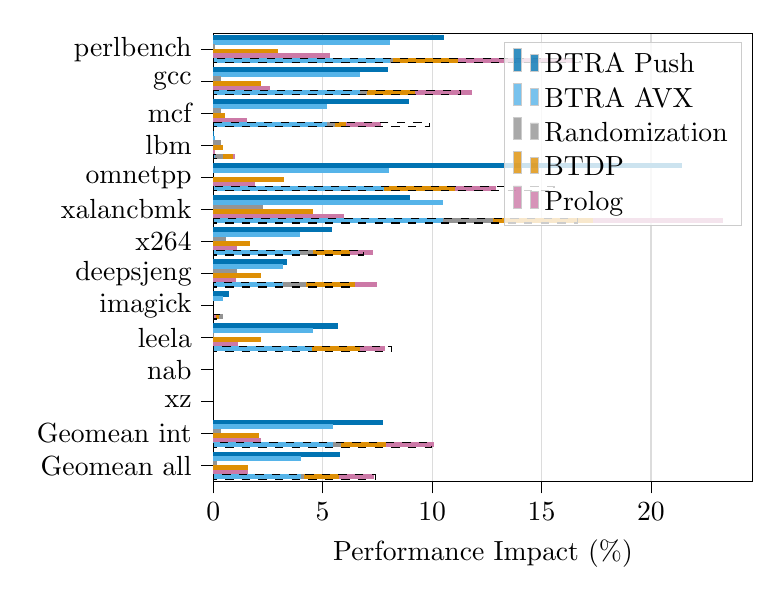
\begin{tikzpicture}

\definecolor{cornflowerblue86180233}{RGB}{86,180,233}
\definecolor{darkcyan1115178}{RGB}{1,115,178}
\definecolor{darkgray176}{RGB}{176,176,176}
\definecolor{darkorange2221435}{RGB}{222,143,5}
\definecolor{gainsboro}{RGB}{220,220,220}
\definecolor{lightgray204}{RGB}{204,204,204}
\definecolor{lightslategray148}{RGB}{148,148,148}
\definecolor{palevioletred204121167}{RGB}{204,121,167}

\begin{axis}[
legend cell align={left},
legend style={fill opacity=0.8, draw opacity=1, text opacity=1, draw=lightgray204},
tick align=outside,
tick pos=left,
x grid style={gainsboro},
xlabel={Performance Impact (\%)},
xmajorgrids,
xmin=0, xmax=24.6524209115605,
xminorgrids,
xtick style={color=black},
y dir=reverse,
y grid style={darkgray176},
ymin=-5.7, ymax=153.9,
ytick style={color=black},
ytick={0,11.4,22.8,34.2,45.6,57,68.4,79.8,91.2,102.6,114,125.4,136.8,148.2},
yticklabels={
  perlbench,
  gcc,
  mcf,
  lbm,
  omnetpp,
  xalancbmk,
  x264,
  deepsjeng,
  imagick,
  leela,
  nab,
  xz,
  Geomean int,
  Geomean all
}
]
\draw[draw=none,fill=darkcyan1115178,line width=0.32pt] (axis cs:0,-4.95) rectangle (axis cs:10.5228359849995,-3.15);
\addlegendimage{ybar,ybar legend,draw=none,fill=darkcyan1115178,line width=0.32pt}
\addlegendentry{BTRA Push}

\draw[draw=none,fill=cornflowerblue86180233,line width=0.32pt] (axis cs:0,-3.33) rectangle (axis cs:8.09050512054441,-1.53);
\addlegendimage{ybar,ybar legend,draw=none,fill=cornflowerblue86180233,line width=0.32pt}
\addlegendentry{BTRA AVX}

\draw[draw=none,fill=lightslategray148,line width=0.32pt] (axis cs:0,-1.71) rectangle (axis cs:0.102948929324365,0.0900000000000001);
\addlegendimage{ybar,ybar legend,draw=none,fill=lightslategray148,line width=0.32pt}
\addlegendentry{Randomization}

\draw[draw=none,fill=darkorange2221435,line width=0.32pt] (axis cs:0,-0.0900000000000001) rectangle (axis cs:2.97203800961976,1.71);
\addlegendimage{ybar,ybar legend,draw=none,fill=darkorange2221435,line width=0.32pt}
\addlegendentry{BTDP}

\draw[draw=none,fill=palevioletred204121167,line width=0.32pt] (axis cs:0,1.53) rectangle (axis cs:5.35259283761467,3.33);
\addlegendimage{ybar,ybar legend,draw=none,fill=palevioletred204121167,line width=0.32pt}
\addlegendentry{Prolog}

\draw[draw=none,fill=darkcyan1115178,line width=0.32pt] (axis cs:0,6.45) rectangle (axis cs:7.96325776259705,8.25);
\draw[draw=none,fill=cornflowerblue86180233,line width=0.32pt] (axis cs:0,8.07) rectangle (axis cs:6.6939967341326,9.87);
\draw[draw=none,fill=lightslategray148,line width=0.32pt] (axis cs:0,9.69) rectangle (axis cs:0.351202653711336,11.49);
\draw[draw=none,fill=darkorange2221435,line width=0.32pt] (axis cs:0,11.31) rectangle (axis cs:2.18395916562102,13.11);
\draw[draw=none,fill=palevioletred204121167,line width=0.32pt] (axis cs:0,12.93) rectangle (axis cs:2.57369055410064,14.73);
\draw[draw=none,fill=darkcyan1115178,line width=0.32pt] (axis cs:0,17.85) rectangle (axis cs:8.92510353542455,19.65);
\draw[draw=none,fill=cornflowerblue86180233,line width=0.32pt] (axis cs:0,19.47) rectangle (axis cs:5.20708257351787,21.27);
\draw[draw=none,fill=lightslategray148,line width=0.32pt] (axis cs:0,21.09) rectangle (axis cs:0.359103405511307,22.89);
\draw[draw=none,fill=darkorange2221435,line width=0.32pt] (axis cs:0,22.71) rectangle (axis cs:0.522618429165012,24.51);
\draw[draw=none,fill=palevioletred204121167,line width=0.32pt] (axis cs:0,24.33) rectangle (axis cs:1.56491259628919,26.13);
\draw[draw=none,fill=darkcyan1115178,line width=0.32pt] (axis cs:0,29.25) rectangle (axis cs:-0.029786244163843,31.05);
\draw[draw=none,fill=cornflowerblue86180233,line width=0.32pt] (axis cs:0,30.87) rectangle (axis cs:0.0947903644594739,32.67);
\draw[draw=none,fill=lightslategray148,line width=0.32pt] (axis cs:0,32.49) rectangle (axis cs:0.335593269580903,34.29);
\draw[draw=none,fill=darkorange2221435,line width=0.32pt] (axis cs:0,34.11) rectangle (axis cs:0.464828414673724,35.91);
\draw[draw=none,fill=palevioletred204121167,line width=0.32pt] (axis cs:0,35.73) rectangle (axis cs:0.0925057204712143,37.53);
\draw[draw=none,fill=darkcyan1115178,line width=0.32pt] (axis cs:0,40.65) rectangle (axis cs:21.4138493018017,42.45);
\draw[draw=none,fill=cornflowerblue86180233,line width=0.32pt] (axis cs:0,42.27) rectangle (axis cs:8.01729948053602,44.07);
\draw[draw=none,fill=lightslategray148,line width=0.32pt] (axis cs:0,43.89) rectangle (axis cs:-0.209019693539614,45.69);
\draw[draw=none,fill=darkorange2221435,line width=0.32pt] (axis cs:0,45.51) rectangle (axis cs:3.21835816884466,47.31);
\draw[draw=none,fill=palevioletred204121167,line width=0.32pt] (axis cs:0,47.13) rectangle (axis cs:1.89522858312223,48.93);
\draw[draw=none,fill=darkcyan1115178,line width=0.32pt] (axis cs:0,52.05) rectangle (axis cs:9.00508911401532,53.85);
\draw[draw=none,fill=cornflowerblue86180233,line width=0.32pt] (axis cs:0,53.67) rectangle (axis cs:10.49317376399,55.47);
\draw[draw=none,fill=lightslategray148,line width=0.32pt] (axis cs:0,55.29) rectangle (axis cs:2.28980619204311,57.09);
\draw[draw=none,fill=darkorange2221435,line width=0.32pt] (axis cs:0,56.91) rectangle (axis cs:4.56331535447239,58.71);
\draw[draw=none,fill=palevioletred204121167,line width=0.32pt] (axis cs:0,58.53) rectangle (axis cs:5.96277351252923,60.33);
\draw[draw=none,fill=darkcyan1115178,line width=0.32pt] (axis cs:0,63.45) rectangle (axis cs:5.41545402201973,65.25);
\draw[draw=none,fill=cornflowerblue86180233,line width=0.32pt] (axis cs:0,65.07) rectangle (axis cs:3.97756917088872,66.87);
\draw[draw=none,fill=lightslategray148,line width=0.32pt] (axis cs:0,66.69) rectangle (axis cs:0.565285394890669,68.49);
\draw[draw=none,fill=darkorange2221435,line width=0.32pt] (axis cs:0,68.31) rectangle (axis cs:1.68927877348599,70.11);
\draw[draw=none,fill=palevioletred204121167,line width=0.32pt] (axis cs:0,69.93) rectangle (axis cs:1.06726179670065,71.73);
\draw[draw=none,fill=darkcyan1115178,line width=0.32pt] (axis cs:0,74.85) rectangle (axis cs:3.3807587361665,76.65);
\draw[draw=none,fill=cornflowerblue86180233,line width=0.32pt] (axis cs:0,76.47) rectangle (axis cs:3.17651406668027,78.27);
\draw[draw=none,fill=lightslategray148,line width=0.32pt] (axis cs:0,78.09) rectangle (axis cs:1.08337644580789,79.89);
\draw[draw=none,fill=darkorange2221435,line width=0.32pt] (axis cs:0,79.71) rectangle (axis cs:2.20518620932224,81.51);
\draw[draw=none,fill=palevioletred204121167,line width=0.32pt] (axis cs:0,81.33) rectangle (axis cs:1.03922921057276,83.13);
\draw[draw=none,fill=darkcyan1115178,line width=0.32pt] (axis cs:0,86.25) rectangle (axis cs:0.717652291506909,88.05);
\draw[draw=none,fill=cornflowerblue86180233,line width=0.32pt] (axis cs:0,87.87) rectangle (axis cs:0.454007645698473,89.67);
\draw[draw=none,fill=lightslategray148,line width=0.32pt] (axis cs:0,89.49) rectangle (axis cs:-0.203708396187241,91.29);
\draw[draw=none,fill=darkorange2221435,line width=0.32pt] (axis cs:0,91.11) rectangle (axis cs:-0.141228659231896,92.91);
\draw[draw=none,fill=palevioletred204121167,line width=0.32pt] (axis cs:0,92.73) rectangle (axis cs:-0.0950377439369876,94.53);
\draw[draw=none,fill=darkcyan1115178,line width=0.32pt] (axis cs:0,97.65) rectangle (axis cs:5.70082551677271,99.45);
\draw[draw=none,fill=cornflowerblue86180233,line width=0.32pt] (axis cs:0,99.27) rectangle (axis cs:4.56437763209439,101.07);
\draw[draw=none,fill=lightslategray148,line width=0.32pt] (axis cs:0,100.89) rectangle (axis cs:-0.0296745319571246,102.69);
\draw[draw=none,fill=darkorange2221435,line width=0.32pt] (axis cs:0,102.51) rectangle (axis cs:2.18982625143276,104.31);
\draw[draw=none,fill=palevioletred204121167,line width=0.32pt] (axis cs:0,104.13) rectangle (axis cs:1.13982237991437,105.93);
\draw[draw=none,fill=darkcyan1115178,line width=0.32pt] (axis cs:0,109.05) rectangle (axis cs:-0.154809113573207,110.85);
\draw[draw=none,fill=cornflowerblue86180233,line width=0.32pt] (axis cs:0,110.67) rectangle (axis cs:-1.41000248078363,112.47);
\draw[draw=none,fill=lightslategray148,line width=0.32pt] (axis cs:0,112.29) rectangle (axis cs:-1.19893496389152,114.09);
\draw[draw=none,fill=darkorange2221435,line width=0.32pt] (axis cs:0,113.91) rectangle (axis cs:-0.075675477496373,115.71);
\draw[draw=none,fill=palevioletred204121167,line width=0.32pt] (axis cs:0,115.53) rectangle (axis cs:-0.369623953580034,117.33);
\draw[draw=none,fill=darkcyan1115178,line width=0.32pt] (axis cs:0,120.45) rectangle (axis cs:-1.32542977772879,122.25);
\draw[draw=none,fill=cornflowerblue86180233,line width=0.32pt] (axis cs:0,122.07) rectangle (axis cs:-0.677246285628041,123.87);
\draw[draw=none,fill=lightslategray148,line width=0.32pt] (axis cs:0,123.69) rectangle (axis cs:-1.24670274020657,125.49);
\draw[draw=none,fill=darkorange2221435,line width=0.32pt] (axis cs:0,125.31) rectangle (axis cs:-0.790459791184694,127.11);
\draw[draw=none,fill=palevioletred204121167,line width=0.32pt] (axis cs:0,126.93) rectangle (axis cs:-0.843564130461361,128.73);
\draw[draw=none,fill=darkcyan1115178,line width=0.32pt] (axis cs:0,131.85) rectangle (axis cs:7.73464891307656,133.65);
\draw[draw=none,fill=cornflowerblue86180233,line width=0.32pt] (axis cs:0,133.47) rectangle (axis cs:5.45903915480244,135.27);
\draw[draw=none,fill=lightslategray148,line width=0.32pt] (axis cs:0,135.09) rectangle (axis cs:0.358832719572444,136.89);
\draw[draw=none,fill=darkorange2221435,line width=0.32pt] (axis cs:0,136.71) rectangle (axis cs:2.07335004102422,138.51);
\draw[draw=none,fill=palevioletred204121167,line width=0.32pt] (axis cs:0,138.33) rectangle (axis cs:2.17431708343636,140.13);
\draw[draw=none,fill=darkcyan1115178,line width=0.32pt] (axis cs:0,143.25) rectangle (axis cs:5.79338123351549,145.05);
\draw[draw=none,fill=cornflowerblue86180233,line width=0.32pt] (axis cs:0,144.87) rectangle (axis cs:3.99133592496594,146.67);
\draw[draw=none,fill=lightslategray148,line width=0.32pt] (axis cs:0,146.49) rectangle (axis cs:0.179214493335755,148.29);
\draw[draw=none,fill=darkorange2221435,line width=0.32pt] (axis cs:0,148.11) rectangle (axis cs:1.57189777483309,149.91);
\draw[draw=none,fill=palevioletred204121167,line width=0.32pt] (axis cs:0,149.73) rectangle (axis cs:1.59476739358766,151.53);
\draw[draw=none,fill=cornflowerblue86180233,line width=0.32pt] (axis cs:0,3.15) rectangle (axis cs:8.09050512054441,4.95);
\draw[draw=none,fill=lightslategray148,line width=0.32pt] (axis cs:8.09050512054441,3.15) rectangle (axis cs:8.19345404986877,4.95);
\draw[draw=none,fill=darkorange2221435,line width=0.32pt] (axis cs:8.19345404986877,3.15) rectangle (axis cs:11.1654920594885,4.95);
\draw[draw=none,fill=palevioletred204121167,line width=0.32pt] (axis cs:11.1654920594885,3.15) rectangle (axis cs:16.5180848971032,4.95);
\draw[draw=none,fill=cornflowerblue86180233,line width=0.32pt] (axis cs:0,14.55) rectangle (axis cs:6.6939967341326,16.35);
\draw[draw=none,fill=lightslategray148,line width=0.32pt] (axis cs:6.6939967341326,14.55) rectangle (axis cs:7.04519938784394,16.35);
\draw[draw=none,fill=darkorange2221435,line width=0.32pt] (axis cs:7.04519938784394,14.55) rectangle (axis cs:9.22915855346496,16.35);
\draw[draw=none,fill=palevioletred204121167,line width=0.32pt] (axis cs:9.22915855346496,14.55) rectangle (axis cs:11.8028491075656,16.35);
\draw[draw=none,fill=cornflowerblue86180233,line width=0.32pt] (axis cs:0,25.95) rectangle (axis cs:5.20708257351787,27.75);
\draw[draw=none,fill=lightslategray148,line width=0.32pt] (axis cs:5.20708257351787,25.95) rectangle (axis cs:5.56618597902918,27.75);
\draw[draw=none,fill=darkorange2221435,line width=0.32pt] (axis cs:5.56618597902918,25.95) rectangle (axis cs:6.08880440819419,27.75);
\draw[draw=none,fill=palevioletred204121167,line width=0.32pt] (axis cs:6.08880440819419,25.95) rectangle (axis cs:7.65371700448338,27.75);
\draw[draw=none,fill=cornflowerblue86180233,line width=0.32pt] (axis cs:0,37.35) rectangle (axis cs:0.0947903644594739,39.15);
\draw[draw=none,fill=lightslategray148,line width=0.32pt] (axis cs:0.0947903644594739,37.35) rectangle (axis cs:0.430383634040377,39.15);
\draw[draw=none,fill=darkorange2221435,line width=0.32pt] (axis cs:0.430383634040377,37.35) rectangle (axis cs:0.8952120487141,39.15);
\draw[draw=none,fill=palevioletred204121167,line width=0.32pt] (axis cs:0.8952120487141,37.35) rectangle (axis cs:0.987717769185315,39.15);
\draw[draw=none,fill=cornflowerblue86180233,line width=0.32pt] (axis cs:0,48.75) rectangle (axis cs:8.01729948053602,50.55);
\draw[draw=none,fill=lightslategray148,line width=0.32pt] (axis cs:8.01729948053602,48.75) rectangle (axis cs:7.80827978699641,50.55);
\draw[draw=none,fill=darkorange2221435,line width=0.32pt] (axis cs:7.80827978699641,48.75) rectangle (axis cs:11.0266379558411,50.55);
\draw[draw=none,fill=palevioletred204121167,line width=0.32pt] (axis cs:11.0266379558411,48.75) rectangle (axis cs:12.9218665389633,50.55);
\draw[draw=none,fill=cornflowerblue86180233,line width=0.32pt] (axis cs:0,60.15) rectangle (axis cs:10.49317376399,61.95);
\draw[draw=none,fill=lightslategray148,line width=0.32pt] (axis cs:10.49317376399,60.15) rectangle (axis cs:12.7829799560331,61.95);
\draw[draw=none,fill=darkorange2221435,line width=0.32pt] (axis cs:12.7829799560331,60.15) rectangle (axis cs:17.3462953105055,61.95);
\draw[draw=none,fill=palevioletred204121167,line width=0.32pt] (axis cs:17.3462953105055,60.15) rectangle (axis cs:23.3090688230348,61.95);
\draw[draw=none,fill=cornflowerblue86180233,line width=0.32pt] (axis cs:0,71.55) rectangle (axis cs:3.97756917088872,73.35);
\draw[draw=none,fill=lightslategray148,line width=0.32pt] (axis cs:3.97756917088872,71.55) rectangle (axis cs:4.54285456577939,73.35);
\draw[draw=none,fill=darkorange2221435,line width=0.32pt] (axis cs:4.54285456577939,71.55) rectangle (axis cs:6.23213333926538,73.35);
\draw[draw=none,fill=palevioletred204121167,line width=0.32pt] (axis cs:6.23213333926538,71.55) rectangle (axis cs:7.29939513596602,73.35);
\draw[draw=none,fill=cornflowerblue86180233,line width=0.32pt] (axis cs:0,82.95) rectangle (axis cs:3.17651406668027,84.75);
\draw[draw=none,fill=lightslategray148,line width=0.32pt] (axis cs:3.17651406668027,82.95) rectangle (axis cs:4.25989051248816,84.75);
\draw[draw=none,fill=darkorange2221435,line width=0.32pt] (axis cs:4.25989051248816,82.95) rectangle (axis cs:6.4650767218104,84.75);
\draw[draw=none,fill=palevioletred204121167,line width=0.32pt] (axis cs:6.4650767218104,82.95) rectangle (axis cs:7.50430593238316,84.75);
\draw[draw=none,fill=cornflowerblue86180233,line width=0.32pt] (axis cs:0,94.35) rectangle (axis cs:0.454007645698473,96.15);
\draw[draw=none,fill=lightslategray148,line width=0.32pt] (axis cs:0.454007645698473,94.35) rectangle (axis cs:0.250299249511232,96.15);
\draw[draw=none,fill=darkorange2221435,line width=0.32pt] (axis cs:0.250299249511232,94.35) rectangle (axis cs:0.109070590279337,96.15);
\draw[draw=none,fill=palevioletred204121167,line width=0.32pt] (axis cs:0.109070590279337,94.35) rectangle (axis cs:0.0140328463423489,96.15);
\draw[draw=none,fill=cornflowerblue86180233,line width=0.32pt] (axis cs:0,105.75) rectangle (axis cs:4.56437763209439,107.55);
\draw[draw=none,fill=lightslategray148,line width=0.32pt] (axis cs:4.56437763209439,105.75) rectangle (axis cs:4.53470310013726,107.55);
\draw[draw=none,fill=darkorange2221435,line width=0.32pt] (axis cs:4.53470310013726,105.75) rectangle (axis cs:6.72452935157002,107.55);
\draw[draw=none,fill=palevioletred204121167,line width=0.32pt] (axis cs:6.72452935157002,105.75) rectangle (axis cs:7.86435173148439,107.55);
\draw[draw=none,fill=cornflowerblue86180233,line width=0.32pt] (axis cs:0,117.15) rectangle (axis cs:-1.41000248078363,118.95);
\draw[draw=none,fill=lightslategray148,line width=0.32pt] (axis cs:-1.41000248078363,117.15) rectangle (axis cs:-2.60893744467515,118.95);
\draw[draw=none,fill=darkorange2221435,line width=0.32pt] (axis cs:-2.60893744467515,117.15) rectangle (axis cs:-2.68461292217153,118.95);
\draw[draw=none,fill=palevioletred204121167,line width=0.32pt] (axis cs:-2.68461292217153,117.15) rectangle (axis cs:-3.05423687575156,118.95);
\draw[draw=none,fill=cornflowerblue86180233,line width=0.32pt] (axis cs:0,128.55) rectangle (axis cs:-0.677246285628041,130.35);
\draw[draw=none,fill=lightslategray148,line width=0.32pt] (axis cs:-0.677246285628041,128.55) rectangle (axis cs:-1.92394902583461,130.35);
\draw[draw=none,fill=darkorange2221435,line width=0.32pt] (axis cs:-1.92394902583461,128.55) rectangle (axis cs:-2.71440881701931,130.35);
\draw[draw=none,fill=palevioletred204121167,line width=0.32pt] (axis cs:-2.71440881701931,128.55) rectangle (axis cs:-3.55797294748067,130.35);
\draw[draw=none,fill=cornflowerblue86180233,line width=0.32pt] (axis cs:0,139.95) rectangle (axis cs:5.45903915480244,141.75);
\draw[draw=none,fill=lightslategray148,line width=0.32pt] (axis cs:5.45903915480244,139.95) rectangle (axis cs:5.81787187437488,141.75);
\draw[draw=none,fill=darkorange2221435,line width=0.32pt] (axis cs:5.81787187437488,139.95) rectangle (axis cs:7.8912219153991,141.75);
\draw[draw=none,fill=palevioletred204121167,line width=0.32pt] (axis cs:7.8912219153991,139.95) rectangle (axis cs:10.0655389988355,141.75);
\draw[draw=none,fill=cornflowerblue86180233,line width=0.32pt] (axis cs:0,151.35) rectangle (axis cs:3.99133592496594,153.15);
\draw[draw=none,fill=lightslategray148,line width=0.32pt] (axis cs:3.99133592496594,151.35) rectangle (axis cs:4.1705504183017,153.15);
\draw[draw=none,fill=darkorange2221435,line width=0.32pt] (axis cs:4.1705504183017,151.35) rectangle (axis cs:5.74244819313479,153.15);
\draw[draw=none,fill=palevioletred204121167,line width=0.32pt] (axis cs:5.74244819313479,151.35) rectangle (axis cs:7.33721558672245,153.15);
\draw[draw=black,dashed] (axis cs:0,3.24) rectangle (axis cs:16.7569149267538,4.86);
\draw[draw=black,dashed] (axis cs:0,14.64) rectangle (axis cs:11.2952207585287,16.26);
\draw[draw=black,dashed] (axis cs:0,26.04) rectangle (axis cs:9.86311885819027,27.66);
\draw[draw=black,dashed] (axis cs:0,37.44) rectangle (axis cs:0.227547204198286,39.06);
\draw[draw=black,dashed] (axis cs:0,48.84) rectangle (axis cs:15.5682312732366,50.46);
\draw[draw=black,dashed] (axis cs:0,60.24) rectangle (axis cs:16.6303425352307,61.86);
\draw[draw=black,dashed] (axis cs:0,71.64) rectangle (axis cs:6.88269310214402,73.26);
\draw[draw=black,dashed] (axis cs:0,83.04) rectangle (axis cs:6.30077796906123,84.66);
\draw[draw=black,dashed] (axis cs:0,94.44) rectangle (axis cs:0.327088091908423,96.06);
\draw[draw=black,dashed] (axis cs:0,105.84) rectangle (axis cs:8.15781053170261,107.46);
\draw[draw=black,dashed] (axis cs:0,117.24) rectangle (axis cs:-0.62458622352014,118.86);
\draw[draw=black,dashed] (axis cs:0,128.64) rectangle (axis cs:-0.379151137889988,130.26);
\draw[draw=black,dashed] (axis cs:0,140.04) rectangle (axis cs:9.98814855472583,141.66);
\draw[draw=black,dashed] (axis cs:0,151.44) rectangle (axis cs:7.39476375402615,153.06);
\end{axis}

\end{tikzpicture}
}%
    \endgroup    \caption{The component-wise overhead of \rtwoc{}'s components.
    See \cref{r2c:sss:eval-btra}, \cref{r2c:sss:eval-heapbt} and \cref{r2c:sss:eval-layout} for details.
    The overhead is relative to the baseline without \rtwoc{}.
    Measurements were performed on \propername{EPYC}.}
    \label{r2c:fig:perf-components}
\end{figure}

In contrast to the \code{push} instructions, setting up 10 \glspl{BTRA} with AVX2 instructions requires only 7 instructions (see \cref{r2c:ss:impl-btras}).
Each block of 4 addresses requires one AVX2 instruction to load them into a register and one to write them onto the stack.
\cref{r2c:fig:perf-components} shows that the optimization improves the overhead caused by \glspl{BTRA} over all benchmarks by 2 percent points.
Most importantly, the optimization decreases the overhead of the outlier \propername{omnetpp} by about 13 absolute percent points, down to 8\%.
In this configuration, the maximum overhead of 10\% is caused by \propername{xalancbmk}.

To analyze the overhead of \cfs (see \cref{r2c:sss:stack-arguments}), we built a configuration without applying any diversification measure, but with \cfs \emph{enabled}.
Enabling only \cfs allows us to measure its performance impact, and the missed opportunities of the frame-pointer omission optimization.
We found that the resulting geometric mean performance overhead is \geomeancfs with a maximum impact of \maxoverheadcfs.
These numbers suggest that the majority of the overhead is caused by writing the \glspl{BTRA} to the stack.


\subsubsection{\glspl{heapbt}}\label{r2c:sss:eval-heapbt}

\begin{figure}[t]
    \centering
    \begingroup
    \pgfplotsset{
        every axis/.append style={
            yticklabel style={font=\propernamedecl\footnotesize},
            execute at begin axis={
                \pgfplotsset{
                    width=\textwidth,
                    height=0.8\linewidth}
            },
        },
    }
    \resizebox{\textwidth}{!}{% This file was created with matplot2tikz v0.4.2.
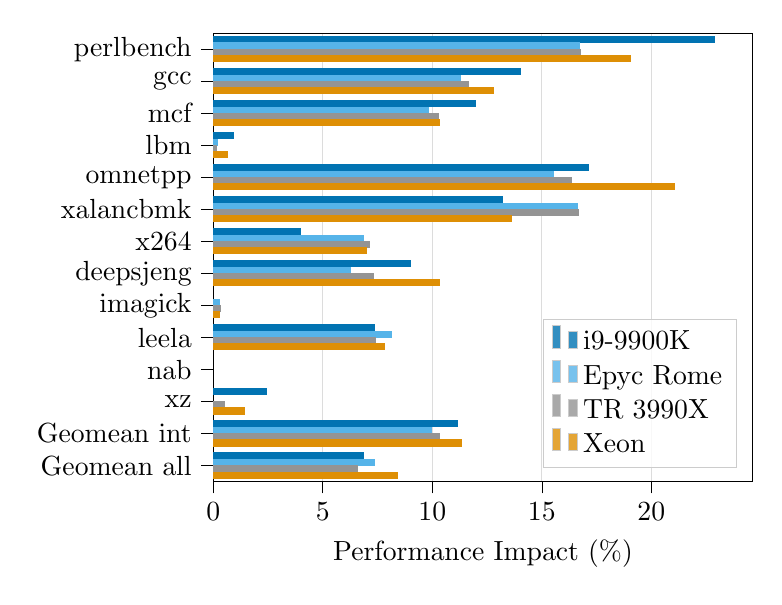
\begin{tikzpicture}

\definecolor{cornflowerblue86180233}{RGB}{86,180,233}
\definecolor{darkcyan1115178}{RGB}{1,115,178}
\definecolor{darkgray176}{RGB}{176,176,176}
\definecolor{darkorange2221435}{RGB}{222,143,5}
\definecolor{gainsboro}{RGB}{220,220,220}
\definecolor{lightgray204}{RGB}{204,204,204}
\definecolor{lightslategray148}{RGB}{148,148,148}

\begin{axis}[
legend cell align={left},
legend style={
  fill opacity=0.8,
  draw opacity=1,
  text opacity=1,
  at={(0.97,0.03)},
  anchor=south east,
  draw=lightgray204
},
tick align=outside,
tick pos=left,
x grid style={gainsboro},
xlabel={Performance Impact (\%)},
xmajorgrids,
xmin=0, xmax=24.6339961082686,
xminorgrids,
xtick style={color=black},
y dir=reverse,
y grid style={darkgray176},
ymin=-4.08, ymax=110.16,
ytick style={color=black},
ytick={0,8.16,16.32,24.48,32.64,40.8,48.96,57.12,65.28,73.44,81.6,89.76,97.92,106.08},
yticklabels={
  perlbench,
  gcc,
  mcf,
  lbm,
  omnetpp,
  xalancbmk,
  x264,
  deepsjeng,
  imagick,
  leela,
  nab,
  xz,
  Geomean int,
  Geomean all
}
]
\draw[draw=none,fill=darkcyan1115178,line width=0.32pt] (axis cs:0,-3.33) rectangle (axis cs:22.8868728825438,-1.53);
\addlegendimage{ybar,ybar legend,draw=none,fill=darkcyan1115178,line width=0.32pt}
\addlegendentry{i9-9900K}

\draw[draw=none,fill=cornflowerblue86180233,line width=0.32pt] (axis cs:0,-1.71) rectangle (axis cs:16.7569149267538,0.0900000000000001);
\addlegendimage{ybar,ybar legend,draw=none,fill=cornflowerblue86180233,line width=0.32pt}
\addlegendentry{Epyc Rome}

\draw[draw=none,fill=lightslategray148,line width=0.32pt] (axis cs:0,-0.0900000000000001) rectangle (axis cs:16.8038011920932,1.71);
\addlegendimage{ybar,ybar legend,draw=none,fill=lightslategray148,line width=0.32pt}
\addlegendentry{TR 3990X}

\draw[draw=none,fill=darkorange2221435,line width=0.32pt] (axis cs:0,1.53) rectangle (axis cs:19.0731603607468,3.33);
\addlegendimage{ybar,ybar legend,draw=none,fill=darkorange2221435,line width=0.32pt}
\addlegendentry{Xeon}

\draw[draw=none,fill=darkcyan1115178,line width=0.32pt] (axis cs:0,4.83) rectangle (axis cs:14.0450537040183,6.63);
\draw[draw=none,fill=cornflowerblue86180233,line width=0.32pt] (axis cs:0,6.45) rectangle (axis cs:11.2952207585287,8.25);
\draw[draw=none,fill=lightslategray148,line width=0.32pt] (axis cs:0,8.07) rectangle (axis cs:11.6585751865229,9.87);
\draw[draw=none,fill=darkorange2221435,line width=0.32pt] (axis cs:0,9.69) rectangle (axis cs:12.7996766901981,11.49);
\draw[draw=none,fill=darkcyan1115178,line width=0.32pt] (axis cs:0,12.99) rectangle (axis cs:11.9920579890501,14.79);
\draw[draw=none,fill=cornflowerblue86180233,line width=0.32pt] (axis cs:0,14.61) rectangle (axis cs:9.86311885819027,16.41);
\draw[draw=none,fill=lightslategray148,line width=0.32pt] (axis cs:0,16.23) rectangle (axis cs:10.3171873907563,18.03);
\draw[draw=none,fill=darkorange2221435,line width=0.32pt] (axis cs:0,17.85) rectangle (axis cs:10.3658053647033,19.65);
\draw[draw=none,fill=darkcyan1115178,line width=0.32pt] (axis cs:0,21.15) rectangle (axis cs:0.952682519924042,22.95);
\draw[draw=none,fill=cornflowerblue86180233,line width=0.32pt] (axis cs:0,22.77) rectangle (axis cs:0.227547204198286,24.57);
\draw[draw=none,fill=lightslategray148,line width=0.32pt] (axis cs:0,24.39) rectangle (axis cs:0.167724868513996,26.19);
\draw[draw=none,fill=darkorange2221435,line width=0.32pt] (axis cs:0,26.01) rectangle (axis cs:0.679115900161542,27.81);
\draw[draw=none,fill=darkcyan1115178,line width=0.32pt] (axis cs:0,29.31) rectangle (axis cs:17.1498282914226,31.11);
\draw[draw=none,fill=cornflowerblue86180233,line width=0.32pt] (axis cs:0,30.93) rectangle (axis cs:15.5682312732366,32.73);
\draw[draw=none,fill=lightslategray148,line width=0.32pt] (axis cs:0,32.55) rectangle (axis cs:16.3933840735117,34.35);
\draw[draw=none,fill=darkorange2221435,line width=0.32pt] (axis cs:0,34.17) rectangle (axis cs:21.0953074822708,35.97);
\draw[draw=none,fill=darkcyan1115178,line width=0.32pt] (axis cs:0,37.47) rectangle (axis cs:13.2106412464191,39.27);
\draw[draw=none,fill=cornflowerblue86180233,line width=0.32pt] (axis cs:0,39.09) rectangle (axis cs:16.6303425352307,40.89);
\draw[draw=none,fill=lightslategray148,line width=0.32pt] (axis cs:0,40.71) rectangle (axis cs:16.6827678304087,42.51);
\draw[draw=none,fill=darkorange2221435,line width=0.32pt] (axis cs:0,42.33) rectangle (axis cs:13.6502610201018,44.13);
\draw[draw=none,fill=darkcyan1115178,line width=0.32pt] (axis cs:0,45.63) rectangle (axis cs:4.0021259106342,47.43);
\draw[draw=none,fill=cornflowerblue86180233,line width=0.32pt] (axis cs:0,47.25) rectangle (axis cs:6.88269310214402,49.05);
\draw[draw=none,fill=lightslategray148,line width=0.32pt] (axis cs:0,48.87) rectangle (axis cs:7.15800878109507,50.67);
\draw[draw=none,fill=darkorange2221435,line width=0.32pt] (axis cs:0,50.49) rectangle (axis cs:6.99999430082181,52.29);
\draw[draw=none,fill=darkcyan1115178,line width=0.32pt] (axis cs:0,53.79) rectangle (axis cs:9.03135163641451,55.59);
\draw[draw=none,fill=cornflowerblue86180233,line width=0.32pt] (axis cs:0,55.41) rectangle (axis cs:6.30077796906123,57.21);
\draw[draw=none,fill=lightslategray148,line width=0.32pt] (axis cs:0,57.03) rectangle (axis cs:7.33675961216422,58.83);
\draw[draw=none,fill=darkorange2221435,line width=0.32pt] (axis cs:0,58.65) rectangle (axis cs:10.3637937448286,60.45);
\draw[draw=none,fill=darkcyan1115178,line width=0.32pt] (axis cs:0,61.95) rectangle (axis cs:-3.48273235558078,63.75);
\draw[draw=none,fill=cornflowerblue86180233,line width=0.32pt] (axis cs:0,63.57) rectangle (axis cs:0.327088091908423,65.37);
\draw[draw=none,fill=lightslategray148,line width=0.32pt] (axis cs:0,65.19) rectangle (axis cs:0.364197863129845,66.99);
\draw[draw=none,fill=darkorange2221435,line width=0.32pt] (axis cs:0,66.81) rectangle (axis cs:0.329224164470721,68.61);
\draw[draw=none,fill=darkcyan1115178,line width=0.32pt] (axis cs:0,70.11) rectangle (axis cs:7.38961334587653,71.91);
\draw[draw=none,fill=cornflowerblue86180233,line width=0.32pt] (axis cs:0,71.73) rectangle (axis cs:8.15781053170261,73.53);
\draw[draw=none,fill=lightslategray148,line width=0.32pt] (axis cs:0,73.35) rectangle (axis cs:7.44074750702926,75.15);
\draw[draw=none,fill=darkorange2221435,line width=0.32pt] (axis cs:0,74.97) rectangle (axis cs:7.84597997176371,76.77);
\draw[draw=none,fill=darkcyan1115178,line width=0.32pt] (axis cs:0,78.27) rectangle (axis cs:-12.0555916319535,80.07);
\draw[draw=none,fill=cornflowerblue86180233,line width=0.32pt] (axis cs:0,79.89) rectangle (axis cs:-0.62458622352014,81.69);
\draw[draw=none,fill=lightslategray148,line width=0.32pt] (axis cs:0,81.51) rectangle (axis cs:-11.5601370968125,83.31);
\draw[draw=none,fill=darkorange2221435,line width=0.32pt] (axis cs:0,83.13) rectangle (axis cs:-0.586622687852534,84.93);
\draw[draw=none,fill=darkcyan1115178,line width=0.32pt] (axis cs:0,86.43) rectangle (axis cs:2.44178427320745,88.23);
\draw[draw=none,fill=cornflowerblue86180233,line width=0.32pt] (axis cs:0,88.05) rectangle (axis cs:-0.379151137889988,89.85);
\draw[draw=none,fill=lightslategray148,line width=0.32pt] (axis cs:0,89.67) rectangle (axis cs:0.561134004435138,91.47);
\draw[draw=none,fill=darkorange2221435,line width=0.32pt] (axis cs:0,91.29) rectangle (axis cs:1.46630841417743,93.09);
\draw[draw=none,fill=darkcyan1115178,line width=0.32pt] (axis cs:0,94.59) rectangle (axis cs:11.1854352509048,96.39);
\draw[draw=none,fill=cornflowerblue86180233,line width=0.32pt] (axis cs:0,96.21) rectangle (axis cs:9.98814855472583,98.01);
\draw[draw=none,fill=lightslategray148,line width=0.32pt] (axis cs:0,97.83) rectangle (axis cs:10.3598398758856,99.63);
\draw[draw=none,fill=darkorange2221435,line width=0.32pt] (axis cs:0,99.45) rectangle (axis cs:11.3721724463311,101.25);
\draw[draw=none,fill=darkcyan1115178,line width=0.32pt] (axis cs:0,102.75) rectangle (axis cs:6.89240575278629,104.55);
\draw[draw=none,fill=cornflowerblue86180233,line width=0.32pt] (axis cs:0,104.37) rectangle (axis cs:7.39476375402615,106.17);
\draw[draw=none,fill=lightslategray148,line width=0.32pt] (axis cs:0,105.99) rectangle (axis cs:6.62388933065103,107.79);
\draw[draw=none,fill=darkorange2221435,line width=0.32pt] (axis cs:0,107.61) rectangle (axis cs:8.45098262457327,109.41);
\end{axis}

\end{tikzpicture}
}%
    \endgroup    \caption{The performance impact of full protection with \rtwoc on four different machines (see \cref{r2c:sss:full-overhead}).}
    % \propername{Geomean int} shows the geometric mean overhead of the SPEC CPU 2017 integer benchmarks only and \propername{geomean all} of the entire benchmark suite.}
    \label{r2c:fig:perf-full}
\end{figure}

We configured \rtwoc{} to insert between zero and five \glspl{heapbt} per function, but disabled other diversification measures.
\cref{r2c:fig:perf-components} shows that the geometric mean overhead of \glspl{heapbt} is 2\% with \propername{xalancbmk} causing the maximum overhead of 5\%.
The optimization to insert \glspl{heapbt} only in functions that write to their stack frame improves performance by 1\%.

\subsubsection{Prolog \& Layout Randomization}\label{r2c:sss:eval-layout}
We also isolated the performance impact of prolog trap insertion, and code- and data-layout randomization techniques---i.e., stack slot shuffling, global variable shuffling, and register-allocation randomization.
The prolog insertion randomly inserts between one and five traps into each function prolog, causing a geometric mean overhead of 2\%, with \propername{xalancbmk} being most affected at 6\%.
The combination of layout randomization techniques generally caused negligible overhead.

% \vspace*{-1em}

\subsubsection{Full \rtwoc}\label{r2c:sss:full-overhead}
We built a configuration with all \rtwoc{} protections enabled (see \cref{r2c:fig:perf-full}).
% would be nice to reiterate, but space is precious
This configuration
\begin{enumerate*}[label={(\roman*)}]
    \item protects return addresses with \glspl{BTRA} (see \cref{r2c:ss:impl-btras});
    \item injects \glspl{heapbt} (see \cref{r2c:ss:impl-heap-boobytraps});
    \item performs stack slot shuffling, global variable shuffling and register-allocation randomization;
    \item and inserts traps into function prologs and NOPs at call sites (see \cref{r2c:ss:strengthening}).
\end{enumerate*}
The geometric mean overhead is similar on all systems, with the \propername{Xeon} machine showing the highest overhead at 8.5\% for the full benchmark suite.
In \cref{r2c:fig:perf-components} the stacked bars (bars with differently colored sections) show the summed component overhead.
To contrast this artificially summed overhead with the actual overhead of all components working together, the dashed bars in \cref{r2c:fig:perf-components} show the real overhead for full \rtwoc on \propername{EPYC}.
For most benchmarks, the sum of component overheads accurately predicts the actual total overhead.
For \propername{mcf} and \propername{omnetpp}, however, the actual overhead is higher than the sum of components and for \propername{xalancbmk} it is lower.

Some benchmarks show diverging results on different machines.
On \propername{i9-9900K}, \propername{perlbench} has a significantly higher overhead than on the other machines.
For \propername{omnetpp}, the \propername{Xeon} machine has the highest overhead at 21\%.
Conversely, \propername{xalancbmk} shows better results on \propername{i9-9900K} and \propername{Xeon} than on the AMD machines.

On \propername{i9-9900K}, we found the webserver throughput \emph{decrease} to be 13\% for \propername{nginx} and 12\% for \propername{Apache}.
On the AMD machines, the throughput decrease was between 3 and 4 percent for both \propername{nginx} and \propername{Apache}.

%    \subsubsection{Adaptive parameter selection}\label{r2c:sss:adaptive}
%    To demonstrate the advantages of adaptive security, we built two configurations with adaptive parameter selection based on performance profiles.
%    Note that the performance profiles also influence LLVM's optimization decisions.
%    For that reason we compared the configurations with adaptive parameter selection to a (faster) profile-enabled baseline.
%    The configuration \propername{Adaptive-PR1} uses the parameter range $[0,2]$ for the lower bound, and the range $[2,5]$ for the upper bound of the subsequent random trial.
%    As a result, the random trial for the coolest call site samples from $[2,5]$ and for the hottest call sites from $[0,2]$ (see \cref{r2c:ss:impl-pgo} for the details).
%    The configuration \propername{Adaptive-PR2} provides better probabilistic security by using larger parameter ranges.
%    Specifically, \propername{Adaptive-PR2} uses a range of $[1,5]$ for the lower bound, and a range of $[2,10]$ for the upper bound.
%    The resulting random trial range for the coolest call sites is $[5,10]$ and for the hottest call sites $[1,2]$.
%    \propername{Adaptive-PR2} differs from \propername{Adaptive-PR1} by allowing twice as many BTRAs in the cold call sites, and protecting even hot call sites with at least \emph{two} BTRAs (also see~\Cref{r2c:fig:average-decoy-counts} for BTRA distribution).
%
%    \rtwoc's use of performance profiles positively influences performance in two ways.
%    First, performance profiles allow for more aggressive inlining:
%    Inlined call sites have no return address and, therefore, also do not need BTRAs.
%    Second, the profiles allow \rtwoc to decrease the number of BTRAs for hot call sites.
%    To evaluate these two effects separately, we built a configuration that uses a fixed number of ten BTRAs in total \emph{despite} the availability of performance profiles, thus cancelling out the effect of adaptive parameter selection.
%    From the comparison we can see that adaptive parameter selection still increases performance over the \propername{Fixed} configuration already optimized with inlining.


\subsubsection{Memory overhead}
To evaluate \rtwoc{}'s memory overhead we linked the benchmark programs from the SPEC CPU 2017 suite to a static library that prints the \propername{maxrss rusage} metric once the program ends.
The \propername{maxrss} metric is the maximum resident-set size of a process during its lifetime.
We chose this methodology because it allows measuring the memory overhead without impacting the benchmark performance.
With this methodology, we found the memory overhead of the SPEC benchmarks to be 1-3\%.

For the webserver benchmarks we had to choose a different methodology because the webservers spawn child processes.
With child processes, \propername{maxrss} reflects the maximum usage among all child processes instead of the combined maximum usage.
Instead, we started a separate monitoring process that records the RSS usage of each webserver process every second and calculated the median.
With this methodology, we found the memory overhead of the webserver benchmarks to be about 100\%.
We verified experimentally that about 55\% of the memory overhead is caused by the page allocations for \glspl{heapbt}.
The rest is caused by \glspl{BTRA} and the increased binary size.

\subsection{Scalability}\label{r2c:ss:scalability}
Although the SPEC benchmark suite covers a wide variety of test programs, we also compiled real-world software with \rtwoc.
Apart from Apache and nginx, we also compiled the GTK version of WebKit~\cite{Webkit} and Chromium~\cite{Chromium}.
We built both browsers with a fixed total number of 10 \glspl{BTRA} per call site.
WebKit and Chromium are massive \cpp projects with more than 4.5 million lines and almost 32 million lines of C/C\plusplus code, respectively.

To verify that \rtwoc does not introduce errors into the browser, we ran the included tests as well as the Speedometer browser benchmark.
To pass the tests, we had to modify a single source file in Chromium, and three source files in Webkit to deactivate \rtwoc for a few functions.
In both cases, unprotected code called an \rtwoc compiled function with stack arguments.
An example is the following function signature from WebKit's \propername{WebCore} module:
\begin{minted}[breaklines]{cpp}
static void gbkCallbackEscape(const void* context, UConverterFromUnicodeArgs* fromUArgs, const UChar* codeUnits, int32_t length, UChar32 codePoint, UConverterCallbackReason reason, UErrorCode* error);
\end{minted}
WebKit registers this function as a callback in the ICU unicode library.
The function has more parameters than can be passed in registers and, thus, needs stack arguments.
Unless the ICU library is compiled with \rtwoc, the calling code does perform \cfs (see \cref{r2c:sss:stack-arguments}).
We discuss this implementation limitation in \cref{r2c:ss:abi-change}.
We did not include the Speedometer performance results in the performance evaluation since Speedometer's results showed a variation of more than 20\% even in the baseline.
In daily browsing we did not notice any difference.

%%% Local Variables:
%%% mode: latex
%%% TeX-master: "../eurosys22"
%%% End:

\section{Discussion}\label{sec:r2c:discussion}
%\begin{figure}[t!]
%  \centering
%  \input{stats/20220519-boxplot-variance-diff-horizontal.pgf}
%  \caption{Performance impact variance of differently diversified variants on selected benchmarks on our \textsf{TR 3970X} A system.}
%  \label{r2c:fig:intra-variant-difference}
%\end{figure}

\subsection{Performance}\label{r2c:ss:discussion-evaluation}

\fbetodo{Add perf counter discussion}
\fbetodo{Add section about profile-guided optimization}
\begin{table}[t]
    \sisetup{
        table-alignment-mode=none,
        table-number-alignment=right,
    }
    \begin{tabular}{lS[table-format=8.0]}
        \toprule
        Benchmark              & {Call Frequency} \\
        \midrule
        \propername{perlbench} & 9435182963       \\
        \propername{gcc}       & 7471474392       \\
        \propername{mcf}       & 38657893688      \\
        \propername{lbm}       & 20906700         \\
        \propername{omnetpp}   & 23536583520      \\
        \propername{xalancbmk} & 12430137048      \\
        \propername{x264}      & 3400115007       \\
        \propername{deepsjeng} & 11366032234      \\
        \propername{imagick}   & 10441212712      \\
        \propername{leela}     & 13108456661      \\
        \propername{nab}       & 135237228510     \\
        \propername{xz}        & 3287645643       \\
        \bottomrule
    \end{tabular}
    \caption{Median call frequencies of SPEC CPU 2017 benchmarks across all inputs.}
    \label{tab:call-frequencies}
\end{table}


\begin{table}[t]
    \centering
    \caption{\Gls{BTRA} overhead by step count. Cycles column shows overhead in percent.}
    \label{tab:btra-overhead}
    \footnotesize
    \setlength{\tabcolsep}{4pt}
    \begin{tabular}{l *{6}{rr}}
        \toprule
        & \multicolumn{2}{c}{2 BTRAs} & \multicolumn{2}{c}{6 BTRAs} & \multicolumn{2}{c}{10 BTRAs} & \multicolumn{2}{c}{14 BTRAs} & \multicolumn{2}{c}{18 BTRAs} & \multicolumn{2}{c}{22 BTRAs} \\
        \cmidrule(lr){2-3} \cmidrule(lr){4-5} \cmidrule(lr){6-7} \cmidrule(lr){8-9} \cmidrule(lr){10-11} \cmidrule(lr){12-13}
        Benchmark & Cycles & IPC & Cycles & IPC & Cycles & IPC & Cycles & IPC & Cycles & IPC & Cycles & IPC \\
        \midrule
        \fileInput{generated/r2c/btra-step-cycles}
        \bottomrule
    \end{tabular}
\end{table}

As evidenced by the benchmarks, the optimized \gls{BTRA} setup sequence improves \rtwoc{}'s performance considerably (see \cref{r2c:fig:perf-components}).
While our implementation uses AVX2 vector instructions, falling back to SSE vector instructions would be an alternative for more feature constrained CPUs.
For CPU's without vector extensions the \code{push} based setup sequence provides a viable alternative without loss of security.
The difference between the \code{push} and AVX2 setup sequence (see \cref{r2c:fig:perf-components}) indicates that increased instruction cache pressure contributes to the overhead.
Similarly, prolog trap insertion also contributes to the increased instruction cache pressure.

% We speculate that at the other end of the spectrum an implementation with AVX512 registers could improve performance even more.
% We could not evaluate this effect due to the lack of compatible hardware.

\Cref{r2c:fig:perf-full} shows that benchmarks with a large number of functions and function calls are affected most by \rtwoc{}.
\rtwoc{} adds \glspl{BTRA} \emph{per call site}, explaining the overhead for function heavy benchmarks.
To test this correlation with call frequency, we instrumented the SPEC CPU benchmark programs to count the number of executed call instructions.
Our instrumentation ignores tail calls because tail calls do not push a return address to the stack and, thus, no \glspl{BTRA} are inserted.
\Cref{tab:call-frequencies} shows the median number of calls performed by the SPEC CPU 2017 benchmarks.
For each benchmark we took the median call frequencies across all inputs.
The data suggests that there is only a weak direct correlation between calls and the overhead:
\propername{Perlbench}, for example, has less than half the number of calls as \propername{omnetpp}, but shows a similar overhead.
The mere call count, therefore, does not sufficiently explain the performance profile.

A possible explanation for the super-additive overhead (sum of component-overheads is less than actual total overhead) in \propername{mcf} and \propername{omnetpp} are memory stalls.
Both \propername{mcf} and \propername{omnetpp} are memory-bound benchmarks and memory stalls can hide a certain number of additional instructions.
Thus, the stalls might hide the instructions of each component in isolation, but the stalls might be too few to hide all components combined.

\subsubsection{Detailed Performance Counter Analysis}
\begin{figure}[t]
    \centering
    \begingroup
    \pgfplotsset{
        every axis/.append style={
            yticklabel style={font=\footnotesize},
            xticklabel style={font=\footnotesize},
            execute at begin axis={
                \pgfplotsset{
                    width=\textwidth,
                    height=0.8\linewidth}
            },
        },
    }
    \input{figures/r2c/btra-instr-vs-cycles}%
    \endgroup
    \caption{The relationship between instruction overhead and cycle overhead.}
    \label{r2c:fig:btra-instr-vs-cycles}
\end{figure}

The example of call count and performance overhead differences between \propername{perlbench} and \propername{omnetpp} above showed that instructions and call counts alone give an incomplete picture.
To better understand the exact causes of the overhead, we recorded \code{perf} counters for particularly affected benchmarks on \propername{i9}.
We choose \propername{i9} instead of \propername{EPYC} for the \code{perf} analysis because of the richer set of performance counters on the Intel machine.
As expected, each benchmark shows a significant increase in the number of instructions.
Most of \rtwoc's diversification measures, \ie prolog trap insertion, \code{NOP} insertion, \glspl{BTRA} and \glspl{heapbt}, require additional instructions.
Additional instructions can affect execution performance in at least two ways:
\begin{enumerate*}
    \item Executing an instruction requires \gls{CPU} cycles.
    This effect is particularly pronounced in hot code;
    \item Additional instructions change the code geometry and increase instruction cache pressure.
    Thus, additional instructions can influence other code parts, even if they are not executed at all.
\end{enumerate*}
Conversely, additional instructions do not necessarily lead to more cycles, as sometimes they can hide in stalls.
The relationship between an increase in instructions and an increase in cycles (if any), thus, can give us a first hint of a benchmark's performance profile.
Given that \glspl{BTRA} are responsible for most of the additional instructions, we performed a series of experiments with all of \rtwoc's defenses in place, but a varying number of \glspl{BTRA}, ranging from 4 to 24.
\cref{r2c:fig:btra-instr-vs-cycles} shows the relation between the cycle overhead and instruction overhead for increasing numbers of \glspl{BTRA}.
\propername{Perlbench}, for example, shows an almost perfectly linear correlation, meaning that each additional instruction also requires a proportional number of additional cycles.

For benchmarks below the diagonal, an additional instruction takes less than one cycle, on average.
This phenomenon can happen, for example, through memory stalls.
Memory stalls enable the \gls{CPU} to execute other instructions in the speculation window \enquote{for free}, while waiting for the fulfillment of the memory request.
Whether an instruction can hide in such a stall window depends on whether the instruction lands in a speculation window including a stall.
For example, if the \glspl{BTRA} setup sequence is preceded by a stalling instruction, the \glspl{BTRA} execute essentially for free (not account for stalls the \glspl{BTRA} themselves might cause).
If no such stalling instruction exists in the \glspl{BTRA}'s proximity, the \glspl{BTRA} execution delays the execution of other instructions.
In benchmarks with memory stalls, thus, \glspl{BTRA} cost fewer cycles on average.
For example, for \propername{mcf} we observe that while, relative to the baseline, instructions increase by almost 60\%, cycles increase only by about 17\%.
This indicates that stalls can absorb many of the additional instructions, explaining at least in part the relatively low overhead of \propername{mcf}.
\propername{Omnetpp} shows a similar picture, with instructions increasing by 60\%, but cycles increasing only by about 26\%.

For \propername{deepsjeng}, which is also below the diagonal but closer to it than \eg \propername{omnetpp} and \propername{mcf}, the hiding effect is less pronounced.
In particular, \rtwoc causes about 17\% more instructions but only 12\% more cycles.
The relatively low performance overhead of \propername{deepsjeng} is better explained by its low \emph{call density}, \ie the ratio of calls to baseline instructions.
\Cref{tab:call-density} shows that \propername{deepsjeng} has the lowest call density (7.0 calls per 1000 instructions) because it executes about 143 instructions between calls on average.
In contrast, \propername{mcf} and \propername{omnetpp} call functions every 43 and 36 instructions respectively, resulting in call densities of 23.5 and 27.5.
Since each call adds approximately 25 \gls{BTRA} instructions, the instruction overhead is roughly proportional to call density.
This explains why \propername{deepsjeng} has only 17\% instruction overhead despite executing more total calls than \propername{perlbench} (11.4B vs 9.4B): the fixed \gls{BTRA} cost is amortized over more baseline work.

\begin{table}[t]
    \centering
    \caption{Call density analysis. Density is calls per 1000 baseline instructions; higher density means more \gls{BTRA} overhead per unit of work.}
    \label{tab:call-density}
    \sisetup{
        table-alignment-mode=none,
        table-number-alignment=right,
    }
    \begin{tabular}{l
        S[table-format=4.1]
        S[table-format=2.1]
        S[table-format=2.1]}
        \toprule
        Benchmark              & {Baseline Instr (B)} & {Calls (B)} & {Density} \\
        \midrule
        \propername{deepsjeng} & 1635.1               & 11.4        & 7.0       \\
        \propername{perlbench} & 829.1                & 9.4         & 11.4      \\
        \propername{gcc}       & 651.7                & 7.5         & 11.5      \\
        \propername{xalancbmk} & 879.8                & 12.4        & 14.1      \\
        \propername{mcf}       & 1645.8               & 38.7        & 23.5      \\
        \propername{omnetpp}   & 857.3                & 23.5        & 27.5      \\
        \bottomrule
    \end{tabular}
\end{table}

Surprised by the difference of memory overhead between SPEC CPU 2017 benchmarks and webserver benchmarks, we verified the memory SPEC results by applying the same methodology as for the webserver benchmarks.
Instead of relying on the \propername{maxrss} counter, we recorded the RSS usage of the SPEC benchmarks with a separate monitoring process.
The results confirmed a memory overhead of only a few percent.
We suspect that for the SPEC benchmarks, memory overhead caused by \rtwoc{} is low compared to the memory consumed by the benchmark itself.
Further research is necessary to substantiate these suspicions.

%The overhead of \glspl{heapbt} and \glspl{BTRA} is mostly independent.
%Only in the case of \propername{omnetpp} is the combined overhead of \glspl{heapbt} and the AVX setup sequence bigger than the sum of the component overheads.
%The overhead of \glspl{heapbt} varies less per benchmark, whereas \glspl{BTRA} affect different benchmarks to different degrees.
%These changes in overhead can be attributed to the fact that \glspl{BTRA} are inserted \emph{per call site}.
%As a result, benchmarks with a large number of function calls are affected more by \glspl{BTRA}.
% Interestingly, despite using the hardened pointer array (see~\ref{r2c:ss:impl-heap-boobytraps}), the variant \propername{AVX2+H\heapbt} shows a slightly improved performance on three benchmarks compared to \propername{AVX2+\heapbt}.
% We suspect an improved cache locality of the pointer array with other data to be responsible for the improvement.

%The performance difference on our benchmark environment illustrated in \Cref{r2c:fig:perf-full} warranted further investigation.
%To account for the randomness invariably introduced by the diversification of the individual benchmark programs, we generated 25 variants of each program and measured their runtime performance impact.
%\Cref{r2c:fig:intra-variant-difference} shows these data and indicates that the performance can depend significantly on the diversification process.
%If users require peak performance, compiling multiple variants and selecting the one with the lowest performance impact is a viable option.

\subsection{Security}\label{r2c:ss:discussion-security}

\begin{table}[t]
    \centering
    \caption{Empirical distribution of function pointers per stack frame.}
    \label{r2c:tab:func-ptr-dist}
    \begin{tabular}{c rr rr rr}
        \toprule
        & \multicolumn{2}{c}{\propername{nginx}} & \multicolumn{2}{c}{\propername{Apache}} & \multicolumn{2}{c}{\propername{Lighttpd}} \\
        \cmidrule(lr){2-3} \cmidrule(lr){4-5} \cmidrule(lr){6-7}
        Count & Frames & \%   & Frames & \%   & Frames & \%   \\
        \midrule
        0     & 74     & 18.5 & 266    & 54.4 & 96     & 25.3 \\
        1     & 174    & 43.5 & 193    & 39.5 & 99     & 26.1 \\
        2     & 122    & 30.5 & 22     & 4.5  & 48     & 12.6 \\
        3     & 23     & 5.8  & 3      & 0.6  & 27     & 7.1  \\
        4     & 5      & 1.3  & 2      & 0.4  & 18     & 4.7  \\
        5     & 2      & 0.5  & 2      & 0.4  & 12     & 3.2  \\
        6     & 0      & 0.0  & 1      & 0.2  & 6      & 1.6  \\
        7     & 0      & 0.0  & 0      & 0.0  & 9      & 2.4  \\
        8     & 0      & 0.0  & 0      & 0.0  & 6      & 1.6  \\
        9     & 0      & 0.0  & 0      & 0.0  & 6      & 1.6  \\
        10    & 0      & 0.0  & 0      & 0.0  & 3      & 0.8  \\
        11+   & 0      & 0.0  & 0      & 0.0  & 50     & 13.2 \\
        \bottomrule
    \end{tabular}
\end{table}

\begin{table}[t]
    \centering
    \caption{\gls{heapbt} single-guess success probabilities for a random stack snapshot.
    Each stack frame contains three \glspl{heapbt} on average.}
    \label{r2c:tab:heap-ptr-probabilities}
    \begin{tabular}{ll rrr r}
        \toprule
        \textbf{Server} & \textbf{Case} & Depth & Heap Ptr. & \glspl{heapbt} & $P_{Success}$ \\
        \midrule
        \multirow{4}{*}{\propername{nginx}}
        & Worst         & 12    & 40        & 36             & 52.6\%        \\
        & Average       & 22    & 100       & 66             & 60.2\%        \\
        & Median        & 22    & 102       & 66             & 60.7\%        \\
        & Best          & 15    & 74        & 45             & 62.2\%        \\
        \midrule
        \multirow{4}{*}{\propername{Apache}}
        & Worst         & 174   & 194       & 522            & 27.1\%        \\
        & Average       & 140   & 269       & 420            & 39.1\%        \\
        & Median        & 140   & 273       & 420            & 39.4\%        \\
        & Best          & 4     & 29        & 12             & 70.7\%        \\
        \midrule
        \multirow{4}{*}{\propername{Lighttpd}}
        & Worst         & 4     & 4         & 12             & 25.0\%        \\
        & Average       & 5     & 48        & 15             & 71.8\%        \\
        & Median        & 8     & 87        & 24             & 78.4\%        \\
        & Best          & 7     & 116       & 21             & 84.7\%        \\
        \bottomrule
    \end{tabular}
\end{table}

\begin{table}[t]
    \centering
    \caption{Function pointer single-guess success probabilities for a random stack frame.
    Each stack frame contains three fake function pointers.}
    \label{r2c:tab:func-ptr-probabilities}
    \begin{tabular}{ll rr r}
        \toprule
        \textbf{Server} & \textbf{Case} & Real Func. Ptr. & Total Func. Ptr. & $P_{Success}$ \\
        \midrule
        \multirow{4}{*}{\propername{nginx}}
        & Worst         & 24              & 27               & 3.7\%         \\
        & Average       & 2.8             & 5.8              & 17.3\%        \\
        & Median        & 1               & 4                & 25.0\%        \\
        & Best          & 1               & 4                & 25.0\%        \\
        \midrule
        \multirow{4}{*}{\propername{Apache}}
        & Worst         & 18              & 21               & 4.8\%         \\
        & Average       & 1.5             & 4.5              & 22.0\%        \\
        & Median        & 1               & 4                & 25.0\%        \\
        & Best          & 1               & 4                & 25.0\%        \\
        \midrule
        \multirow{4}{*}{\propername{Lighttpd}}
        & Worst         & 72              & 75               & 1.3\%         \\
        & Average       & 19.9            & 22.9             & 4.4\%         \\
        & Median        & 2               & 5                & 20.0\%        \\
        & Best          & 1               & 4                & 25.0\%        \\
        \bottomrule
    \end{tabular}
\end{table}

While execute-only memory and function shuffling defeat classic ROP and JIT-ROP attacks, indirect JIT-ROP and \gls{AOCR} remain an issue.
For an indirect JIT-ROP attack, an attacker needs to locate valid code pointers, such as return addresses, in readable memory and infer gadget locations based on the found pointers.
For an \gls{AOCR} attack, an attacker needs to locate function pointers or infer them from other code pointers (\eg return addresses), as well as manipulate function parameters.
In the following subsections we discuss how \rtwoc{} counters each of these attack vectors.
We also discuss the security of stack unwinding tables and the possibility of an attacker corrupting entire or partial code pointers.

Our security evaluation relies on a probabilistic model to estimate an attacker's success rate.
We instantiate the model's variables (such as stack frame composition and pointer distribution) with empirical measurements from \propername{nginx}, \propername{Apache} and \propername{ighttpd}.

\subsubsection{Leaking Return Addresses}\label{r2c:sss:leaking-return-addresses}
\rtwoc protects return addresses with \glspl{BTRA}.
As detailed in \cref{r2c:ss:decoy-mimicry}, the only way for an attacker to identify a return address among the \glspl{BTRA} is by applying brute force.
An attacker's chance to correctly guess the return address depends on the number of \glspl{BTRA} used.
If $B$ is the number of \glspl{BTRA} for a call site, the probability of correctly guessing the return address is given by
\[ P(\mathrm{return address})=\frac{1}{B+1}. \]
Specifically, with 11 \glspl{BTRA} per return address $P(\mathrm{return address})\approx0.09$.
Since return addresses on their own are of limited use, they form only a building block for further inferences.

\subsubsection{Leaking Function Pointers}\label{r2c:sss:leaking-function-pointers}
For an \gls{AOCR}-style whole-function-reuse attack, an attacker needs to locate \emph{specific} function pointers.
That is, the attacker must locate a function pointer with manipulatable parameters and desired functionality.
There are three ways for an attacker to locate function pointers:
\begin{enumerate*}
    \item from the data section;
    \item via the stack, either from function pointers on the stack or indirectly from return addresses
    \item from the heap.
\end{enumerate*}

\rtwoc does not directly protect the heap against information leakage, but aims to prevent an attacker from reaching the heap via the stack via \glspl{heapbt}.
We discuss their respective security properties in \cref{r2c:sss:heap-data}.
\gls{ASLR} randomizes the address of the data section and global-variable shuffling randomizes the order of elements in the data section.
Leaking a function pointer from the data section, therefore, requires a leaked data section pointer first.
Within the data section, an attacker must then locate the desired function pointer.
Exact localization is challenging because of function permutation and boobytrap pointers in the data section.

Leaking a function pointer from the stack can happen either directly or indirectly via a previously leaked return address.
We start with the probability of a direct leak.
Estimating the success probability of locating function pointers on the stack depends on the number of function pointers per stack frame.
Assuming that an attacker can leak arbitrary stack snapshots (see \cref{r2c:s:threat-model}) and can differentiate stack frames within a stack snapshot, stack slot shuffling is currently the only protection.
An attacker can reasonably differentiate function pointers from the return address and \glspl{BTRA} because these occur only at the top of a frame.
With value range analysis an attacker can further differentiate function pointers from other stack slots, such as variables values or heap pointers.
Thus, guessing a function pointer's location means choosing an element from a permutation of all function pointers in the stack frame.
To measure the probability empirically, we have collected stack snapshots from benchmarking workloads on \propername{Apache}, \propername{nginx,} and \propername{lighttp}.
\cref{r2c:tab:func-ptr-dist} shows the function pointer distribution in these snapshots.
About 25\% to 26\% of stack frames (depending on the software) contain no function pointer at all.
In \propername{nginx}, 45\% of all stack frames contain only one function pointer, in \propername{Apache} 35\% and in \propername{lighttp} 14\%.
These cases are troublesome because they mean that an attacker can immediately identify the desired pointer.
Even with two function pointers per frame (between 4.5\% and 30.5\%) the probability of guessing correctly is still 50\%.
We note, however, that only very select function pointers are suitable for \gls{AOCR}'s variant of whole-function-reuse attack and that global variable shuffling further frustrates efforts to locate and manipulate default function parameters.

Leaking a function pointer from a return address requires more guessing.
Let us assume that an attacker has successfully leaked a return address $\mathcal{A}$.
Let us further assume that the attacker \emph{knows} that $\mathcal{A}$ points into a function $\mathcal{F}$.
The attacker can then try to guess the entrypoint of $\mathcal{F}$ for a whole-function-reuse attack.
The function's entrypoint is guaranteed to be before $\mathcal{A}$.
Assuming an average function size of $S$, there are on average $\frac{S}{2}$ addresses before a random return site within $\mathcal{F}$.
With a function alignment of $A$ (typically 16), there are, therefore, on average $\frac{S}{2A}$ possible entry points.
\rtwoc{}'s additional code randomization (see \cref{r2c:ss:strengthening}) decreases the success probability further.
With inserted traps, the function's start address does not coincide with the function's entrypoint.
With $T$ inserted trap instructions, an attacker must guess $\frac{S}{2*A} * T$ possible entrypoints.
The probability of correctly guessing the function's entrypoint thus becomes
\[ P(\mathrm{entrypoint})=\frac{2*A}{S*T}. \]
The average function size $S$ depends on the program, the alignment is typically 16, and the average number of traps depends on a configurable parameter in \rtwoc.
For an alignment $A=16$, a median function size of $S=258$ bytes in a protected \propername{nginx} and an average number of prolog traps $T=3$, this means $P(\mathrm{entrypoint})\approx0.04$.
Estimating based on the median function size is conservative, as the average function size in \propername{nginx} is 789 bytes.
The probability for leaking a single function pointer based on a leaked return address is
\[ P(\mathrm{retaddr\rightarrow{}func}) = P(\mathrm{return address}) * P(\mathrm{entrypoint}). \]
With the concrete numbers from above $P(\mathrm{retaddr\rightarrow{}func})\approx0.0038$.

\subsubsection{Leaking Gadget Addresses}
Instead of mounting a whole-function-reuse attack, an attacker can try to leak enough gadget addresses for a \gls{ROP} attack.
Except for completely blind guessing, an attacker can guess gadget addresses relative to an anchor point.
Such an anchor point can either be a leaked function address (see \cref{r2c:sss:leaking-function-pointers}) or a leaked return address (see \cref{r2c:sss:leaking-return-addresses}).
In either case, the attacker knows the number of call sites between the anchor and the gadget of choice, since \rtwoc does not change the number of call sites.
Each call site has $R_{B}$ \glspl{BTRA} and for each \gls{BTRA}, \rtwoc adds a \code{NOP} with a probability of $P_{NOP}$.
The number of \glspl{BTRA} and the probability of inserted \code{NOP}s are configurable parameters in \rtwoc.
Let $C$ be the average number of call sites within a function in the target program.
We can then estimate the number of call sites between the anchor and a gadget address as $C_{between}=\frac{C}{2}$ on average.
$C_{between}$ is, of course, only a rough estimate that highly depends on $C$.
For \propername{nginx}, we found $C$ to be 4 (median) and 7.3 (average).
Based on these variables, we derive that between the anchor and the gadget, there are $C_{between} * R_{B} * P_{NOP}$ \code{NOP}s on average.
The probability of guessing a gadget address thus becomes
\[ P(\mathrm{gadget})=\frac{1}{C_{between}*B*P_{NOP}}. \]
With 11 \glspl{BTRA} per return address, a probability of $P_{NOP}=0.35$ and $C_{between}=2$, which we used for full \rtwoc, we get $P(\mathrm{gadget})\approx13.9$.
Estimating based on the median number of call sites is conservative, as the average number of call sites per function in \propername{nginx} is 7.
Gadget-based attacks are further impeded by register-allocation randomization.

An attacker typically needs more than one gadget, further decreasing the chance of successfully guessing \emph{all} locations.
For example, the probability of leaking two return addresses and within each function two gadgets is
\[ P\left(\mathrm{2retaddrs\rightarrow{}4gadgets}\right) = P(\mathrm{return address})^2 * P(\mathrm{gadget})^4. \]
With the concrete numbers from above this means $P\left(\mathrm{2retaddrs\rightarrow{}4gadgets}\right)\approx0,00017$.

\subsubsection{Leaking Heap Data}\label{r2c:sss:heap-data}
An attacker can try to leak data from the heap to either learn function pointers or pointers leading to the data section.
As \gls{ASLR} randomizes the heap's location, leaking data requires either a heap over-read vulnerability or a heap pointer.
Such a heap pointer can come either from the data section or the stack.
Unlike with function pointers, the attacker can pick an arbitrary heap pointer to reach the heap.
Heap pointers in the data section are rare, which is why we focus our analysis on the stack.

The probability of correctly guessing a benign heap pointer among all heap pointers depends on the number of benign heap pointers $H$, and the number of \glspl{heapbt} $H_{B}$ in a stack dump.
The number of $H_{B}$ in turn depends on the number of stack frames in the dump because \rtwoc inserts \glspl{heapbt} into each stack frame, depending on a configuration parameter (see \cref{r2c:ss:impl-heap-boobytraps}).
The probability of randomly picking a benign pointer is $\frac{H}{H_{B}+H}$.
The exact number for $H$ is application-specific and depends, for example, on the number of registers containing heap pointers that are spilled to the stack.
\cref{r2c:tab:heap-ptr-probabilities} shows the empirical distribution of heap pointers in stack snapshots taken from \propername{Apache}, \propername{nginx}, and \propername{lighttp} during benchmark workloads.
The table also shows the success probability of randomly guessing a heap pointer among all heap pointers found in a randomly chosen stack snapshot.
As the success probability depends on the concrete composition of the stack snapshot, the table shows the worst, average, and best case for the attacker.
Assuming that an attacker can dump arbitrary many stack snapshots (see \cref{r2c:s:threat-model}), the attacker can repeat the leak until he finds a best-case snapshot.
Generally, snapshots with few stack frames but many heap pointers in those frames constitute the best case for the attacker.
Since \rtwoc inserts a configurable number of \glspl{heapbt} \emph{per frame}, stack snapshots with fewer frames contain also fewer \glspl{heapbt}.
\cref{r2c:tab:heap-ptr-probabilities} also shows, however, that even in the worst case (for the attacker), the success probability still ranges between 25\% and 52.6\%.

The numbers above suggest that \glspl{heapbt} offer only limited protection against heap-based attacks.
We discuss a possible extension of the mimicry principle \emph{onto} the heap in \cref{r2c:ss:heap-mimicry}.

Alternatively to guessing a heap pointer, an attacker could try to identify events where \glspl{heapbt} do not mimic their benign counterparts accurately.
For example, by performing heap feng shui an attacker might be able to identify benign heap pointers with a known distance to each other~\cite{Sotirov2007}.
Note, however, that such an attack requires specific prerequisites and goes significantly beyond the analysis steps of the demonstrated \gls{AOCR} attacks.

Given that \glspl{heapbt} incur overhead but affords only limited protection, an alternative use of the underlying implementation could be to write fake code pointers instead.
\glspl{BTRA} already provide the means for code pointers pointing to booby traps and the \glspl{heapbt} implementation way of writing pointers to random stack slots.
The expected overhead would remain the same or be less because the heap is no longer fragmented by guard pages.
In a function-pointer-guessing scenario, however, the afforded security of pointer mimicry is better.
Recall from \cref{r2c:sss:leaking-function-pointers} that when leaking a function pointer, the attacker needs a \emph{specific} pointer within a \emph{specific} stack frame.
Pointer mimicry could thus help in cases where there are only few function pointers in a stack frame and, as a result, stack slot randomization does not sufficiently protect them (see \cref{r2c:tab:func-ptr-dist}).
Analogous to \cref{r2c:tab:heap-ptr-probabilities}, \cref{r2c:tab:func-ptr-probabilities} contains empirical data together with success probabilities for guessing a function pointer, assuming three fake function pointers per frame on average.
Note that unlike \cref{r2c:tab:heap-ptr-probabilities}, \cref{r2c:tab:func-ptr-probabilities} shows data \emph{per frame}.
Whereas without fake function pointers the best case success probability for the attacker was 100\%, the probability with fake pointers drops to 25\%.
Care must be taken, however, not to write fake code pointers into stack frames without real function pointers.
Since an attacker knows which stack frames contain function pointers in the non-randomized binary, the attacker could identify fake pointers in frames that previously did not contain any function pointers.

\subsubsection{Exception handling and stack unwinding}
\fbetodo{extend with example}
As part of the \gls{BTRA} setup and teardown code, \rtwoc{} also emits the necessary \code{CFI} directives to support exception handling and stack unwinding.
\code{CFI} directives record stack pointer and frame modifications in the \code{.eh\_frame} section.
Since the modifications are recorded relative to the beginning of the frame, decoding the \code{.eh\_frame} section could reveal the location of the return address.
Entries in the \code{.eh\_frame} are not, however, associated with function symbols, but with \gls{PC} \emph{ranges}.
These \gls{PC} ranges are unknown to the attacker due to code layout randomization.
An attacker cannot, therefore, associate entries in the \code{.eh\_frame} table with functions.

The position of an entry in the table---i.e., its row---could provide the attacker with important information.
Each entry in the table, reflects the position of a function in a compilation unit.
% Through function reordering/permutation, the attacker is also deprived of this information.
Through function reordering/permutation row-based references become invalid.
Since exceptions occur infrequently, one could also use a more expensive protection scheme, such as encryption, to protect these meta-data.

\subsubsection{Corrupting code pointers}\label{r2c:sss:corrupting-code-pointers}
\fbetodo{extend section}
\Glspl{CRA} typically corrupt entire code pointers.
An attack called \gls{PIROP} generalizes this principle by corrupting only parts of code pointers and, as a result, is immune to ASLR and page-level randomization~\cite{Goktas2018}.
\rtwoc{} impedes a \gls{PIROP} attack in two ways.
First, \rtwoc{} shuffles functions and randomizes at the sub-function level (see \cref{r2c:ss:strengthening}), thus increasing the entropy for \gls{PIROP}.
Second, \glspl{BTRA} constrain candidate \gls{PIROP} gadgets that manipulate (partial) return addresses:
In the presence of \glspl{BTRA} a \gls{PIROP} attack needs to corrupt \emph{all} return addresses, requiring either iterative gadget execution or more complex gadgets.

\subsection{Remaining attack surface}\label{r2c:ss:remaining-attack-surface}
At present, \rtwoc{} remains susceptible to two types of brute force attacks.
In a Blind ROP scenario with restarting worker processes, an attacker could use \gls{PIROP} to brute force the entropy resulting from \rtwoc{} randomization techniques.
Similarly, an attacker could use the corruption of potential return addresses as a side channel.
For example, by overwriting selected return address candidates with zero and observing whether the process crashes, the attacker could learn the location of the real return address.
Both attacks could be prevented by load time re-randomization.

\rtwoc{} could also deter the corruption of \glspl{BTRA} by checking a random subset of \glspl{BTRA} for consistency after the return.

\rtwoc{} focuses on code-reuse attacks and the leakage of \emph{control-flow} data.
Although \rtwoc{}'s layout randomization raises the bar for attackers~\cite{Hu2016}, \rtwoc{} does not offer the same protection as defenses specialized for data-only attacks~\cite{Carr}.

A way to strengthen \rtwoc{}'s security would be to combine it with \gls{MVEE}s~\cite{Cox2006,Berger2006,Bruschi2007,Volckaert2016,Voulimeneas2020}.
\gls{MVEE}s and diversification defenses like \rtwoc{} naturally complement each other.
Considering that \rtwoc{} diversifies along multiple dimensions, an \gls{MVEE} would detect data corruption or leakage in one of the variants with high probability.

\section{Limitations}\label{r2c:ss:limitations}

\subsection{Coverage}\label{r2c:ss:limitations-coverage}
\rtwoc{} is able to protect only the call-sites and functions it actually compiles.
\glspl{BTRA} for calls to unprotected functions are disabled by default as these functions would overwrite all the \glspl{BTRA} after the return address.
Without \glspl{BTRA} after the return address, the return address would always be the last address in the list of addresses.
Overwritten \glspl{BTRA} are only an issue, however, if the attacker knows which parts of the program have not been compiled by \rtwoc.
Lacking this information, an attacker does not know where the return address is the last address.

\subsection{Change of calling convention}\label{r2c:ss:abi-change}
At present, our prototype implementation does not support calling functions with stack arguments from code not compiled by \rtwoc.
This incompatibility is due to such functions expecting the caller to prepare a frame pointer to account for the changed calling convention.
During our evaluation of \rtwoc{}, we encountered just three such cases (one in the unit tests of WebKit, one in the XML parser callbacks of WebKit, and one in the regular expression implementation of Chromium).
With three cases in 35 million lines of C/\cpp code, we conclude that this combination is rare in practice and, thus, opted for disabling the emission of \glspl{BTRA} for the affected functions.
Note that these cases could also be supported by automatically inserting a trampoline for externally visible functions with stack parameters.
% For ease of implementation we simply deactivated DRAs for the affected functions.

\subsection{Probability of Successful Guesses}
\glspl{BTRA} are mainly effective in deterring \emph{multiple} return address leaks, \eg if an attacker wants to infer multiple gadget locations from return addresses.
The reason is that guessing a single address location among the \glspl{BTRA} still leaves the attacker with a reasonably high chance of success.
Specifically, guessing a single return address location among 12 addresses (\ie 11 \glspl{BTRA}) has a success probability of ~9\%.
Increasing the number of \glspl{BTRA} within a single stack frame reduces this probability only marginally.
For example, doubling the number of \glspl{BTRA}, \eg with AVX512 would lead to 23 \glspl{BTRA}, but still a success probability of ~4\%.
Similarly, \glspl{heapbt} would need to outnumber real heap pointers on the stack with a ratio of 1 to 100 to reach a success probability of less than 1\%.

\section{Possible Extensions}

\subsection{Caller and Callee \gls{BTRA} Synchronization}\label{r2c:ss:caller-and-callee-synchronization}
In \cref{r2c:ss:impl-btras} we described how caller and callee have to agree on how much space is needed after the real return address for additional \glspl{BTRA}.
As for indirect calls the compiler cannot always determine the call target, the \rtwoc compiler tolerates occasional \gls{BTRA} overwrites.
A possibility for caller and callee to synchronize at runtime would be to base the position of the real return address on the callee's runtime address.
For example, a simple hash function could transform the caller's runtime address into a value between $0$ and $N+1$, where $N$ is the number of \glspl{BTRA} per function.
Since both the caller and the callee know the callee's address, the caller can choose the right number of \glspl{BTRA} to push and the callee knows the required stack pointer offset.
An added benefit of this approach would be that the position of the real return address changes with each program start.
Even without load-time function permutation, \gls{ASLR} moves function addresses on each program load.


\subsection{Implementation on ARM}
Our implementation of \rtwoc is based on the x86-64 architecture and aims to respect architecture-specific behavior such as that the \code{CALL} instruction automatically pushes the return address onto the stack.
The idiosyncrasy of the \code{CALL} instruction makes the \gls{BTRA} setup challenging.
Specifically, it requires the caller to properly position the stack pointer and the callee to move the stack pointer again to avoid overwriting \glspl{BTRA} (see \cref{r2c:ss:impl-btras}).
On the ARM architecture, where the return address is saved in the \code{LR}, only callees that execute a call themselves have to spill the \code{LR} register.
Spilling in the callee avoids the synchronization problem discussed in \cref{r2c:ss:caller-and-callee-synchronization}, as saving and loading the return address happens in the same function.

Another area where ARM would provide a benefit for \rtwoc over x86-64 are memory tags.
In our current implementation the \glspl{heapbt} use guard pages to cause traps upon access.
Having to allocate full pages for \glspl{heapbt} leads to heap fragmentation and makes \glspl{heapbt} easier to distinguish from regular allocations.
ARM memory tags on the other hand, have a granularity of 16 bytes.
On ARM, the \glspl{heapbt} runtime could tag small allocations on the heap with a memory tag and then use pointers with a \emph{different} tag as \glspl{heapbt}.

\subsection{Heap Mimicry}\label{r2c:ss:heap-mimicry}
As discussed in \cref{r2c:sss:heap-data}, the security guarantees of \glspl{heapbt} are limited.
The heap offers rich information to an adversary: it stores function pointers and other heap references and, in many scenarios, keeping the attacker away from heap memory is impractical.
A different approach is to extend the mimicry principle to the heap.
Similar to the idea of \glspl{BTRA} and \glspl{heapbt}, \rtwoc could penalize attempts to follow pointers of \emph{random} objects on the heap.
\rtwoc could, for instance, allocate a fake heap object for every $X$th real heap object and free one fake object on every $X$th deallocation.
Dereferencing pointers in these fake heap objects would trigger a booby trap.
An advantage of this approach is that the resulting pointers and allocation patterns very closely resemble real allocations.
To further strengthen the illusion of real heap objects, the fake heap objects could change over time, \eg through manipulation by a background thread.
To make this approach practical, two challenges have to be overcome.
First, allocation of these fake objects should not happen in hot code, such as a loop, to avoid excessive performance overhead.
Second, the fake objects should closely resemble the data structures of real heap objects used in the protected program.
For example, if a program only allocates structures with a single function pointer, then fake objects containing multiple function pointers are immediately recognizable to the attacker.
Such data structure imitation could happen based on the types used for real heap allocations.


\subsection{Speculative Booby Traps}\label{r2c:ss:speculative-booby-traps}%

\newsavebox{\speculativebt}
\begin{lrbox}{\speculativebt}

    \begin{lstlisting}[style=asmcode,frame=none,breaklines=false,basicstyle=\scriptsize\ttfamily]
<boobytrap>: |\Circled{1}|
 call set_up_target
|\tikzmark{T-Decoy-Gadget}| jmp F

set_up_target:
 mov (%rsp), target
 ret|\tikzmark{T-Ret-Alarm}|

target:
 call alarm|\tikzmark{T-Call-Alarm}|
    \end{lstlisting}
\end{lrbox}


\begin{figure}[t]
    % --- ROW 1: GRAPHICAL CONTENT ---
    % This row contains the graphics, aligned at their bottom edges.

    \begin{minipage}[b]{0.25\linewidth}
        \begin{lstlisting}[style=asmcode,basicstyle=\footnotesize\ttfamily]
call set_up_target

capture_spec:
 pause
 jmp capture_spec

set_up_target:
 mov (%rsp), %rax
 ret
        \end{lstlisting}
    \end{minipage}%
    \hfill%
    \begin{minipage}[b]{0.7\linewidth}
        \resizebox{\linewidth}{!}{
            \includeDrawioFigure{figures/r2c/btra-only-stack}[remember picture]{
                \node[anchor=north west] (CodeBox) at (Code) {\usebox\speculativebt};
                \draw[dash pattern=on 4pt off 4pt] (CodeBox.north west) rectangle (CodeBox.south east);
                \draw[dash pattern=on 2pt off 2pt] (Bomb) -- (CodeBox.north west);
                \draw[dash pattern=on 2pt off 2pt] (Bomb) -- (CodeBox.south west);
                \draw[-latex, dash dot] ([shift={(-1pt,2pt)}] pic cs:T-Decoy-Gadget) -| (Elbow) |- (ReturnInstr);
                \node[yshift={1.5*\ht\pgfnodeparttextbox}] at (Elbow) {\scriptsize{}\code{\Circled{\ttfamily2}}};
                \coordinate (RetAlarm) at ([shift={(2pt,2pt)}] pic cs:T-Ret-Alarm);
                \coordinate (RightOffset) at ($ (CodeBox.west)!.8!(CodeBox.east) $, 0);
                \coordinate (OffsetPoint) at (RightOffset |- RetAlarm);
                \draw[-latex, solid] (RetAlarm) -- (OffsetPoint) |- ([shift={(2pt,2pt)}] pic cs:T-Call-Alarm);
                \node[shift={(-\ht\pgfnodeparttextbox, -\ht\pgfnodeparttextbox)}] at (OffsetPoint)  {\scriptsize{\Circled{\ttfamily3}}};
            }
        }
    \end{minipage}

    % --- ROW 2: CAPTIONS ---
    % This row contains the captions, aligned at their top edges.
    % The \subcaption command will work inside the minipage.

    \begin{minipage}[t]{0.3\linewidth}
        \subcaption{Retpolines control the branch target speculation for indirect branches.}
        \label{lst:retpoline}
    \end{minipage}%
    \hfill%
    \begin{minipage}[t]{0.6\linewidth}
        \subcaption{A speculation aware booby trap that looks like the expected code during speculative execution.}
        \label{r2c:fig:speculation-aware-boobytrap}
    \end{minipage}
\end{figure}



Booby traps are an effective measure to deter random probing.
For booby traps to be effective, two properties must hold:
\begin{enumerate*}
    \item they must be indistinguishable from benign code from the attacker's perspective and
    \item triggering them must have negative consequences for the attacker.
\end{enumerate*}
Code-layout randomization in combination with execute-only memory ensures the first property.
The negative consequences for the attacker depend on the booby trap used, but can range from simply crashing the program over raising an alarm to launching a counter-attack~\cite{Crane2013}.
These observations hold true, however, only in the non-speculative domain.

Over the last 8 years, transient-execution attacks have opened another battleground besides the classic \glspl{CRA}.
In a transient execution attack an attacker abuses the \gls{CPU}'s speculation behavior to transiently execute potentially harmful code.
Although the code execution is only transient, such speculatively executed code leaves behind traces that an attacker can extract with a variety of methods.\fbetodo{cite cache side channels}
Apart from using this principle to directly leak sensitive information, attackers can also lift \glspl{CRA} into the speculative domain.

The Blindside attack, for example, employs the same principles as Blind ROP to speculatively locate gadgets with a technique called \emph{gadget probing}.
The idea behind gadget probing is that gadgets can be identified by their cache behavior during speculative execution.
Similarly, SpecROP~\cite{Bhattacharyya2020} executes entire gadget chains speculatively.
The speculative execution of gadgets makes these techniques immune to runtime exceptions.

An attacker could use this fault-resistant capability to either leak data or to uncover booby trap addresses.
Assume, for example, that a booby-trap function is located at address \code{0xbeef} and that the adversary leaks a stack frame with \code{0xbeef} occurring as a potential return address.
To avoid detection, the attacker speculatively executes the code at \code{0xbeef} and observes its cache behavior.
Since \code{0xbeef} points to the booby trap, the resulting cache traces differ from those of the actual return site.
Thus, speculative execution poses a threat to boob-trap functions.

Booby traps are vulnerable because
\begin{enumerate*}
    \item they exhibit the \emph{same} behavior in both, speculative and non-speculative execution;
    \item their observable behavior during speculative execution is \emph{different} from benign code.
\end{enumerate*}
Protecting booby traps against speculation requires a new approach.
We call our approach \emph{speculation-aware booby traps}, as it lifts the deceiving properties of booby traps into the speculative domain.
Although we have prototyped speculation-aware booby traps, we did not include them in the final defense, as we considered them out of scope for \rtwoc.
We present the idea here to motivate more research in that direction.

Speculation-aware booby traps build on the principle of separating speculative and non-speculative control flow.
This principle was first demonstrated by retpolines~\cite{Turner2018}, which capture speculative control-flow in a spin loop.
\cref{lst:retpoline} shows an example of a retpoline protecting an indirect branch to the address in \code{rax} against speculative execution.

Instead of a spin loop, speculation-aware booby traps redirect speculative control-flow to the code an attacker expects behind an address.
\cref{r2c:fig:speculation-aware-boobytrap} shows how speculation-aware booby traps could be used in the context of \rtwoc.
For example, if \code{0x400530} is a booby trap address and \code{0x40055d} denotes the real return address, a speculation-aware booby trap would redirect the speculative control flow to \code{0x40055d}.
The cache traces left behind by speculatively executing \code{0x400530} would, thus, reflect those of speculatively executing \code{0x40055d}.
The only way for an attacker to know for sure what code hides behind \code{0x40055d} would be to execute it non-speculatively, which would trigger the booby trap.

\section{Summary}

\rtwoc demonstrates that compiler-driven data randomization can effectively complement existing code randomization techniques.
By disguising return addresses and heap pointers among booby-trapped decoys, \rtwoc raises the cost of reconnaissance attacks while maintaining practical performance overhead.

The defense is not without limitations: coverage depends on compilation scope, and the probabilistic guarantees diminish against attackers with unlimited observations.
Nonetheless, \rtwoc illustrates a broader principle: the compiler's detailed knowledge of program structure---in this case, stack frame geometry---enables security transformations that would be difficult to achieve through post-hoc instrumentation.

The following chapter discusses broader questions about the future of diversity-based defenses and their potential composition with other defense strategies.
\chapter{Outlook}\label{ch:outlook-defense}
\section{Combining Defense Strategies}
In \cref{ch:code-reuse-coevolution} we gave a brief overview of the defensive strategies against \glspl{CRA} that have emerged over time.
The description in \cref{ch:code-reuse-coevolution} already hints at the fact that none of these strategies are a silver bullet.
Each strategy is effectively a compromise between security, performance, and compatibility.
\rtwoc is no exception to this conundrum.

When looking at years of research on \gls{CRA} defenses, it becomes clear that each defense category has different strengths and weaknesses.
The aim of software diversity, for example, is to avoid a \emph{widespread} attack across program instances even if an attacker found an exploitable vulnerability.
In other words, software diversity aims to break the assumption that because an exploit works on one target instance, it also works on another.
If, however, an attacker targets only one particular instance in the first place, an attacker might be willing to accept higher reconnaissance costs and even manual target reconnaissance.
Defending against these types of targeted attacks with software diversity alone becomes increasingly difficult.
On the other hand, software diversity has proven to be effective even against --- at the time the defense was conceived --- unknown attack vectors.
For example, fine-grained code randomization is not only an effective antidote against \glspl{CRA}, but also against certain transient-execution attacks.

In contrast, \gls{CFI} gives non-probabilistic guarantees about the protection afforded.
This principle goes both ways, however.
A weak spot in a program's \gls{CFI} policy, \eg caused by an imprecise \gls{CFG} analysis, affects \emph{all} instances of that program alike.
Similarly, strict memory-safety enforcement, while prohibitively expensive when applied to the whole program, might be necessary only at certain places not covered by cheaper defenses.

Given these mutually exclusive strengths and weaknesses, it is surprising that there is little research on the compositionality of different defense strategies.
While defenses in one category occasionally \enquote{borrow} concepts from another category, \eg \propername{OCFI}, the effectiveness of combining techniques remains unclear.
That is, what are the security guarantees of drawing multiple lines of defense?
A combination of \gls{CFI} and software diversity, for example, could provide the dependable guarantees of \gls{CFI}, while various forms of randomization could plug the holes left by an imprecise \gls{CFI} policy.
Although combined defenses certainly have desirable properties, they are likely to also pose new challenges.
Is the performance overhead of multiple defenses additive, or even worse?
How to combine defenses that are built on different assumptions?
Various forms of \gls{CFI}, for example, read a target marker from an indirect branch target, thus assuming that the code section is readable.
At the same time, a readable code section is an Achilles heel for a randomized code layout, which is why leakage-resilient diversity aims to prevent reads from the code section.
To answer these and other questions, research into the composition of defensive techniques is necessary.

\section{Evaluating Attacks and Defenses}
A crucial aspect of scientific publications is the underpinning of claims with evidence.
Publications about attack techniques typically provide evidence by showing that the attack can successfully bypass certain defenses.
Successful exploitation of a \emph{particular} software package with a \emph{particular} implementation of a defense is no guarantee, however, that the attack's principle is generalizable.
The \gls{AOCR} paper, for example, claims that \gls{AOCR} can bypass several types of pointer hiding and redirection schemes, not just \gls{CPH}.
While this claim might be true in principle, two of the example exploits rely on the ability to reliably infer forward pointers from leaked return addresses.
Such an inference is only possible (at least reliably) due to the specific layout of the \gls{CPH} table.

On the defense side, a sound security evaluation is equally challenging.
Many \gls{CFI} techniques, for example, did not take into account that programs using \code{printf} essentially embed a hard-to-restrict interpreter with powerful capabilities.
Similarly, the Readactor authors speculated about the possibility of a whole-function-reuse attack, but without \gls{AOCR}'s malicious thread blocking and pointer profiling, such an attack was infeasible.
Another issue is the lack of metrics formalizing the security capabilities of a defense.
While metrics such as \gls{AIR}~\cite{zhang2013} and newer variants such as BlockInsulation and CFGInsulation~\cite{frassetto2022} provide a foundation for \gls{CFI}, similar metrics for software diversity are missing.
The \propername{Survivor} algorithm provided a comparable metric for early variants of software diversity focusing on reducing the risk of \gls{ROP} gadgets.
In light of new challenges such as \gls{JITROP} and new diversification techniques that reach far beyond the gadget level a new metric is needed.
Although transformations like function permutation or stack layout randomization allow for localized probability-theoretic arguments, their effect on real attacks remains hard to predict.
Thus, we hope that future researchers take up the challenging of formulating a theory of software diversity


\partintro{%
While the first part of this thesis focused on hardening deployed programs against exploitation, this part addresses the complementary goal of finding bugs before deployment.
Fuzzing has emerged as one of the most effective techniques for discovering vulnerabilities in complex software, but its effectiveness depends critically on the feedback mechanisms that guide input generation.

The compiler is uniquely positioned to provide rich feedback signals.
Beyond the code coverage metrics that most fuzzers rely on, the compiler has access to semantic information about program structure, optimization decisions, and data dependencies.
This part explores two ways to leverage this information.

\Cref{ch:fuzzer-guidance} provides background on fuzzer feedback mechanisms and their limitations.
We then present \lool, a fuzzing framework that uses the compiler's optimization log as a domain-specific coverage metric for compiler testing.
Finally, we introduce \emph{Program State Convolution} (PSC), a technique that uses compiler analyses to project hidden data dependencies onto observable control flow, and present preliminary results exploring its potential.
}
\part{Improving Fuzzer-Guidance with Compiler Assistance}\label{part:fuzzing}
\chapter{Fuzzer Guidance}\label{ch:fuzzer-guidance}

Before presenting our contributions to compiler-assisted fuzzing, this chapter establishes the necessary background on fuzzer feedback mechanisms.
We examine how coverage-guided fuzzers work, how the compiler enables efficient coverage instrumentation, and where current approaches fall short.
These limitations motivate the techniques presented in the following chapters.

At its core, fuzzing is an automated testing technique that repeatedly executes a target program with generated inputs to discover faults.
To maximize the efficiency of this search, modern fuzzers rely on feedback mechanisms that distinguish interesting inputs from redundant ones.
In this chapter we will examine different types of coverage feedback with a particular focus on how the compiler enables them.

Code-coverage feedback---an umbrella term for code coverage variants---is a popular form of fuzzer feedback.
The idea of code coverage was first introduced as part of Microsoft's SAGE fuzzer, a whitebox fuzzer combining symbolic execution with coverage feedback.
It was AFL, however, which popularized the approach for greybox fuzzing by allowing code-coverage to guide the seed selection and mutation process without the overhead of program analysis~\cite{Zalewski2016}.
The tremendous success of AFL in bug finding also seemed to confirm this strategy.

The particular flavor of code coverage used by AFL and many of its descendants is \emph{edge coverage}.
Unlike basic block coverage, which only tracks visited locations, edge coverage records the frequency and direction of \emph{transitions} between basic blocks.
For example, consider three basic blocks $A$, $B$, and $C$.
A valid execution might traverse them in the order $A \rightarrow B \rightarrow C$, while another might execute $A \rightarrow C \rightarrow B$.
A simple basic block coverage metric would register both executions identically, as the set of visited blocks $\{A, B, C\}$ is the same in both cases.
Edge coverage, however, records the specific transitions: tuples $(A, B)$ and $(B, C)$ for the first path, versus $(A, C)$ and $(C, B)$ for the second.
This inclusion of directionality provides a more granular view of the execution flow, allowing the fuzzer to distinguish between differing traversals of the same code regions.

Despite its widespread use and success, edge coverage, and more general code coverage, suffers from conceptual and from implementation issues.
An analysis by \citeauthor{Bohme2022} even suggests that code coverage alone is insufficient to judge a fuzzer's bug-finding performance~\cite{Bohme2022}.

On the implementation side, early inefficiencies present in, \eg AFL were largely solved or at least mitigated with increasingly refined code coverage implementations.
For instance, the initial coverage implementation in AFL modified the assembler to instrument targets.
The instrumentation assigns a pseudorandom ID to each basic block and computes edge IDs at runtime by combining the ID of the previous block with the ID of the current block~\cite{Zalewski2014}:
\begin{center}
\begin{minted}{C}
cur_location = <COMPILE_TIME_RANDOM>;
shared_mem[cur_location ^ prev_location]++;
prev_location = cur_location >> 1;
\end{minted}
\end{center}
The right-shift by one distinguishes edge $A \rightarrow B$ from edge $B \rightarrow A$.
While the implementation in the assembler is conceptually simple, it is prone to hash collisions and prevents the compiler's optimization passes from optimizing the inserted code.
CollAFL reduces AFL's hash collisions by parameterizing the hash function with additional parameters chosen at link time~\cite{Gan2018}.
Other implementations, such as \aflpp, improve on these issues with a full-fledged compiler pass that builds on LLVM's sanitizer instrumentation infrastructure.

The compiler pass allows \aflpp to replace the collision-prone hash function with a single counter-increment per edge location.
An edge location is a location in a basic block that uniquely identifies an edge.
For so-called \emph{critical edges} there is no such unambiguous location.
A critical edge is an edge \emph{from} a basic block with more than one successor \emph{to} a basic block with more than one successor.
For example, consider the critical edge on the left side of \cref{lool:fig:critical-edges}.
The traditional AFL instrumentation would have to identify this edge by combining the edge IDs of BB\textsubscript{0} and BB\textsubscript{3}.
The reason is that no single location in the graph (neither BB\textsubscript{0} nor BB\textsubscript{3}) uniquely identifies the edge BB\textsubscript{0}\rightarrow{}BB\textsubscript{3}.
A counter in BB\textsubscript{0} would trigger also if the edge BB\textsubscript{0}\rightarrow{}BB\textsubscript{2} is visited and a counter in BB\textsubscript{3} when the edge BB\textsubscript{1}\rightarrow{}BB\textsubscript{3} is visited.
While in principle the edge's trip count could be calculated post-hoc, \eg by using Kirchhoff's law, this requires a computationally expensive post-processing step.
Instead, critical-edge splitting allows the compiler to insert a counter into BB\textsubscript{split} that uniquely identifies the edge BB\textsubscript{0}\rightarrow{}BB\textsubscript{3}.

\begin{figure}
    \centering
    \begin{subfigure}[t]{0.45\linewidth}
        \begin{tikzpicture}[
        % Define the style for the basic blocks
            block/.style={
                rectangle,
                draw=black,
                text width=1cm,
                minimum height=1cm,
                align=center,
                rounded corners=8pt,
                font=\sffamily
            },
            arrow/.style={->, >=Latex},
            critical/.style={red}
        ]

            \matrix (m) [
                matrix of nodes,
                nodes={block, anchor=center}, % Apply block style to all nodes
                column sep=2cm, % Horizontal gap between columns
                row sep=3cm     % Vertical gap between rows
            ] {
            % First Row
                BB\textsubscript{0} & BB\textsubscript{1} \\
                % Second Row
                BB\textsubscript{2} & BB\textsubscript{3} \\
            };

            \draw [arrow] (m-1-1.south) -- (m-2-1.north); % BB0 -> BB2
            \draw [arrow] (m-1-2.south) -- (m-2-2.north); % BB1 -> BB3

            \draw [arrow,critical] (m-1-1.south) -- (m-2-2.north); % BB0 -> BB3

        \end{tikzpicture}

    \end{subfigure}
    \begin{subfigure}[t]{0.45\linewidth}
% --- FIGURE 2: CFG with the Critical Edge SPLIT ---
        \begin{tikzpicture}[
            block/.style={
                rectangle,
                draw=black,
                text width=1cm,
                minimum height=1cm,
                align=center,
                rounded corners=8pt,
                font=\sffamily
            },
        % Style for the new split block
            splitblock/.style={
                block,
                fill=red!20, % Different color to highlight it's new
                text width=1cm,
                font=\sffamily\normalsize % Smaller font to fit text
            },
            arrow/.style={->, >=Latex},
            critical/.style={->, >=Latex}
        ]
            \matrix (m) [
                matrix of nodes,
                nodes={block, anchor=center},
                column sep=3cm, % Increased spacing for the new block
                row sep=3cm,
                yshift=-2cm
            ] {
                BB\textsubscript{0} & BB\textsubscript{1} \\
                BB\textsubscript{2} & BB\textsubscript{3} \\
            };

            % Place the new split block between BB0 and BB3
            % We position it relative to the matrix nodes
            \node[splitblock] (split) at ($(m-1-1.south)!0.5!(m-2-2.north)$) {BB\textsubscript{split}};


            % Normal Edges
            \draw [arrow] (m-1-1.south) -- (m-2-1.north);
            \draw [arrow] (m-1-2.south) -- (m-2-2.north);

            % New Edges forming the split path (in red)
            \draw [critical] (m-1-1.south) to[out=-70, in=110] (split.north);

            % Similar angles for the second part to maintain symmetry.
            \draw [critical] (split.south) to[out=-70, in=110] (m-2-2.north);

        \end{tikzpicture}

    \end{subfigure}
    \caption{Splitting of a critical edge (red edge between BB\textsubscript{0} and BB\textsubscript{3}) by inserting a new basic block BB\textsubscript{split}.}
    \label{lool:fig:critical-edges}
\end{figure}

The compiler instrumentation loads the counter through an additional indirection.
This indirection enables the instrumentation to assign a unique sequential ID to each edge at program startup, \ie, at runtime.
A further refinement of coverage instrumentation, based on \gls{LTO}, removes the indirection and assigns collision-free IDs at compile time.
Compile-time ID assignment is possible because with \gls{LTO} the compiler regains a holistic view of the target program.
Knowing the total number of edge IDs at compile time also allows eliminating the counter-load indirection, thus reducing the performance overhead.
The primary downside of this code-coverage implementation compared to earlier implementations is that not all programs compile with \gls{LTO} enabled.
The refinement of coverage implementations through tighter compiler integration further exemplifies the compiler's role in enhancing fuzzing.

Despite these refinements, code coverage instrumentation has a non-negligible overhead that directly impacts fuzzing throughput.
While there are no published detailed analyses of the overhead incurred by different compiler instrumentation techniques, \citeauthor{Nagy2019} reports an overhead ranging between 30\% and 70\%.
This observation is in line with other work that reports speedups of 4\% to 78\% by reducing the amount of instrumentation needed~\cite{hsu2018}.
These numbers refer to compiler instrumentation without \gls{LTO} and can vary for different techniques and runtime environments.
For example, the overhead of dynamic binary instrumentation or instrumenting Java class files is significantly higher, whereas \gls{LTO}-based instrumentation is likely to incur less overhead.
We will return to the issue of code-coverage overhead in \cref{lool:s:evaluation}.

Distinct from the method of instrumentation is the representation of the coverage map itself.
Fuzzer feedback must strike a delicate balance between precision and throughput.
To avoid frequent cache misses, fuzzers typically limit the size of the coverage bitmap to ensure it fits within the \gls{CPU}'s L2 cache.
This hardware-imposed limitation implies that the map can represent only a finite number of counters, and each counter possesses a limited value range.
The standard coverage map size in AFL, for example, is 64KB, with each byte serving as a counter from 0 to 255.
Previous work has demonstrated that the size of the coverage map significantly impacts fuzzing throughput~\cite{Wang2019}.
However, the exact relationship between fuzzing throughput, map size, hardware cache specifics, and counter precision remains a subject of further research~\cite{sarafov2024}.

Beyond implementation constraints, edge coverage suffers from conceptual limitations.
The fundamental issue is that it compresses complex program states into a single, flat metric.
By tracking edges individually, the fuzzer may fail to capture the context or the specific sequence of edges that led to a program state, thereby identifying two semantically different executions as identical.
A natural extension to this principle is to track paths containing more than one edge, sometimes called \emph{n-gram}~\cite{Wang2019}.
With growing $n$, n-grams approximate full program traces.
Another refinement of code coverage is to include caller contexts in the coverage information~\cite{Chen2018a,Wang2019}.
As edge-coverage instrumentation happens only within a function, information about who called the function is lost.
For instance, consider the C code in \cref{cov:lst:caller-context-example}.
The function \texttt{init\_session} executes the exact same control-flow path (and thus generates the exact same edge coverage features) regardless of whether it is called by \texttt{admin\_login} or \texttt{guest\_login}.
However, these two executions represent fundamentally different program states.
If a fuzzer discovers the path through \texttt{admin\_login} first, it may mark the edges inside \texttt{init\_session} as covered and deprioritize exploring the same path via \texttt{guest\_login}, potentially missing bugs that only manifest in the guest context.

\begin{listing}[t]
    \centering
    \begin{minted}{C}
static bool admin = false;
void init_session(char *input) {
  // The control flow here is identical for both callers.
  if (input[0] == 'A') {
      setup_memory(input);
  }
}

void admin_login() {
  admin = true;
  init_session("A...");
}

void guest_login() {
  admin = false;
  init_session("A...");
}
    \end{minted}
    \caption{Example illustrating the loss of caller context.
    The internal edges of \texttt{init\_session} are identical for both callers, masking the difference between admin and guest states.}
    \label{cov:lst:caller-context-example}
\end{listing}
Angora, for example, addresses this issue by augmenting edge-coverage with a call context hash.
The call context hash is the result of XORing unique call-site IDs at runtime.
In \cref{ch:psp} we explore an alternative way to incorporate caller context by projecting the context onto code coverage with a compiler transformation.

Researchers have also proposed alternative types of coverage feedback that are not based on code coverage.
The goal of these coverage metrics is to improve the fuzzer's ability to differentiate program states.
\citeauthor{Wang2019} tried to formalize this notion with a metric called \emph{sensitivity}, offering a theoretical framework to evaluate the descriptive power of different coverage variants~\cite{Wang2019}.
The authors also propose an early form of dataflow coverage based on the memory access patterns caused by a particular input.
Unfortunately, later proposed coverage metrics have not been evaluated within the same theoretical framework, making a direct comparison difficult.
DDFuzz~\cite{Mantovani2022} and DAFL~\cite{Kim2023}, for instance, use data-dependency information as coverage feedback.
Similarly, \citeauthor{herrera2023} investigate fuzzer guidance by different granularities of dataflow information~\cite{herrera2023}.

In \cref{ch:lool} we introduce a new form of coverage feedback for compiler fuzzing that incurs less overhead than code coverage, while allowing for more context sensitivity.


\chapter{Fuzzer-Guidance with Optimization-Log Counters}\label{ch:lool}
\section{Introduction}

The previous chapter established that code coverage, while effective, provides an incomplete view of program behavior.
This chapter presents \lool, an approach tailored specifically to compiler testing that addresses these limitations by using the compiler's own optimization log as a coverage signal.

Despite being complex software themselves, the correctness of compilers is even more important than the correctness of other software, given that bugs in the compiler can silently propagate to every program it compiles.
Yet testing compilers is challenging precisely because the interesting behaviors (optimization interactions, corner cases in code generation) are difficult to trigger with random inputs and difficult to detect with generic coverage metrics.

\lool addresses this challenge by leveraging a unique property of compilers: they already record which optimizations they perform.
By treating these optimization events as coverage features, \lool can guide input generation toward rare optimization combinations that are likely to expose bugs.

\pgfplotsset{
    optimizationchart/.style={
        width=0.9\textwidth,
        height=13cm,
        xlabel={Count},
        ylabel={},
        yticklabel style={font=\footnotesize\propernamedecl},
        y axis line style={opacity=0},
        axis x line*=bottom,
        tick align=outside,
        enlarge y limits={0.03},
        bar width=10pt,
        y=14pt,
        xminorticks=false,
        axis lines*=left,
    },
    optimizationbar/.style={
        fill=gray!20,
        draw=black,
        line width=0.4pt,
    },
}
\tikzset{
    optimizationlabel/.style={
        anchor=center,
        font=\footnotesize,
    },
}
\begin{figure}[t]
    \centering
    \resizebox{\textwidth}{!}{% Auto-generated by optimizationcounts.py
% Customize styles in importing document:
%   \pgfplotsset{optimizationbar/.style={...}}
%   \tikzset{optimizationlabel/.style={...}}
\begin{tikzpicture}
\begin{axis}[
    xbar,
    xmode=log,
    xmin=10,
    ytick=data,
    yticklabels={
        CanonicalReplacement,
        FixedWithFloatingReplacement,
        Duplication,
        DeoptimizeToGuardConversion,
        GuardElimination,
        LoopPeeling,
        LoopCounterStampImprovement,
        PhiImprovement,
        EqualityPropagation,
        LoopVectorization,
        SequentialIfElimination,
        NodeDeduplication,
        InvertedLoopPhiFreeing,
        LoopFullUnroll,
        PreMainPostInsertion,
        LoopReadWithPhiReplacement,
        DeoptimizeMovement,
        LoopInversion,
        BinaryCanonicalization,
        ConstantReassociation,
        CfgSimplificationCustom,
        OptimisticMemoryEdgeInsertion,
        IndexedLoadElimination,
        BoxNodeBoxUsageReplacement,
        NodeNarrowing,
        PiImprovement,
        UnsignedDivOptimized,
        LockCoarsening,
        NestedLockElimination,
        IndexedStoreElimination,
        LoopRotation,
        CircularPhiBreakerInsertion,
        ExitEnterElimination,
        ExitControlSplitEnterElimination,
        InfeasibleBranchElimination
    },
    optimizationchart,  % apply custom style
]
\addplot+[optimizationbar] coordinates {
    (12458851,0)
    (1383318,1)
    (508643,2)
    (269648,3)
    (198137,4)
    (143313,5)
    (109909,6)
    (81501,7)
    (52872,8)
    (34188,9)
    (32244,10)
    (23596,11)
    (15155,12)
    (13074,13)
    (7154,14)
    (7077,15)
    (5902,16)
    (5745,17)
    (5306,18)
    (4489,19)
    (3831,20)
    (3021,21)
    (2957,22)
    (2851,23)
    (2014,24)
    (1264,25)
    (634,26)
    (401,27)
    (323,28)
    (136,29)
    (129,30)
    (84,31)
    (53,32)
    (27,33)
    (11,34)
};

% Centered labels (positions pre-calculated)
\node[optimizationlabel] at (axis cs:11161.92,0) {\num{12458851}};
\node[optimizationlabel] at (axis cs:3719.30,1) {\num{1383318}};
\node[optimizationlabel] at (axis cs:2255.31,2) {\num{508643}};
\node[optimizationlabel] at (axis cs:1642.10,3) {\num{269648}};
\node[optimizationlabel] at (axis cs:1407.61,4) {\num{198137}};
\node[optimizationlabel] at (axis cs:1197.13,5) {\num{143313}};
\node[optimizationlabel] at (axis cs:1048.37,6) {\num{109909}};
\node[optimizationlabel] at (axis cs:902.78,7) {\num{81501}};
\node[optimizationlabel] at (axis cs:727.13,8) {\num{52872}};
\node[optimizationlabel] at (axis cs:584.71,9) {\num{34188}};
\node[optimizationlabel] at (axis cs:567.84,10) {\num{32244}};
\node[optimizationlabel] at (axis cs:485.76,11) {\num{23596}};
\node[optimizationlabel] at (axis cs:389.29,12) {\num{15155}};
\node[optimizationlabel] at (axis cs:361.58,13) {\num{13074}};
\node[optimizationlabel] at (axis cs:267.47,14) {\num{7154}};
\node[optimizationlabel] at (axis cs:266.03,15) {\num{7077}};
\node[optimizationlabel] at (axis cs:242.94,16) {\num{5902}};
\node[optimizationlabel] at (axis cs:239.69,17) {\num{5745}};
\node[optimizationlabel] at (axis cs:230.35,18) {\num{5306}};
\node[optimizationlabel] at (axis cs:211.87,19) {\num{4489}};
\node[optimizationlabel] at (axis cs:195.73,20) {\num{3831}};
\node[optimizationlabel] at (axis cs:173.81,21) {\num{3021}};
\node[optimizationlabel] at (axis cs:171.96,22) {\num{2957}};
\node[optimizationlabel] at (axis cs:168.85,23) {\num{2851}};
\node[optimizationlabel] at (axis cs:141.92,24) {\num{2014}};
\node[optimizationlabel] at (axis cs:112.43,25) {\num{1264}};
\node[optimizationlabel] at (axis cs:79.62,26) {\num{634}};
\node[optimizationlabel] at (axis cs:63.32,27) {\num{401}};
\node[optimizationlabel] at (axis cs:56.83,28) {\num{323}};
\node[optimizationlabel] at (axis cs:36.88,29) {\num{136}};
\node[optimizationlabel] at (axis cs:35.92,30) {\num{129}};
\node[optimizationlabel] at (axis cs:28.98,31) {\num{84}};
\node[optimizationlabel] at (axis cs:23.02,32) {\num{53}};
\node[optimizationlabel] at (axis cs:16.43,33) {\num{27}};
\node[optimizationlabel] at (axis cs:10.49,34) {\num{11}};
\end{axis}
\end{tikzpicture}}
    \caption{Counts of selected optimizations during the compilation of \num{1000} fuzzed test cases (logarithmic axis).}\label{lool:fig:optimizations}
\end{figure}

Bugs in compilers can have a significant impact on users, especially when the symptom is not a crash, but a silent miscompilation.
Determining that a suspected program bug actually is a miscompilation is a time-consuming process for software developers.
Hand-written tests for the compiler, such as unit tests for specific components, typically cover cases the compiler engineer already considers during development, but edge cases are often overlooked.

The GraalVM compiler, a compiler for Java and other languages (\cref{lool:s:graalvm}), serves as both an \gls{AOT} and \gls{JITcomp}.
As such, bugs in the GraalVM compiler potentially have a far-reaching effect and are particularly problematic.
Being written entirely in Java, the GraalVM compiler is not affected by memory safety issues plaguing compilers written in C or \cpp.
Nonetheless, the GraalVM compiler is not immune to implementation errors, occasionally leading to miscompilations or failed assertions that lead to a crash.
An effective way to compensate for the blind spot of hand-written tests is fuzzing in general and \emph{compiler fuzzing} in particular.
Compiler fuzzing aims to cover the missing test scenarios by feeding random inputs to the compiler.
We developed a compiler fuzzing framework targeting the GraalVM compiler and, in line with related work~\cite{yang2011}, found several previously unknown bugs.

The sustained effectiveness of a compiler fuzzer depends on the capabilities of the input code generator.
The generator can trigger certain compiler optimizations only with very specific combinations of language features.
A naïve input generation approach uses a fixed probability distribution of language features to include.
A problem with this approach, however, is the small probability of certain language feature combinations occurring in a test program of limited size.
If these combinations are necessary to trigger a specific optimization, the optimization remains untested with a high probability.
Optimization frequencies vary: some trigger frequently, while others trigger only rarely.
\cref{lool:fig:optimizations} shows the execution counts for certain optimizations we recorded for one fuzzing campaign with~1000 randomly generated Java programs using the code generator's default configuration.
The least frequent optimization in this data set occurs~11 times overall.
In contrast, other optimizations occur hundreds of thousands or even millions of times on the same \num{1000} test programs.
These data suggest that the GraalVM fuzzer would profit from fuzzer guidance.

In \cref{ch:fuzzer-guidance}, we discussed how feedback can transform random exploration into a more efficient, guided process.
While code coverage is a popular form of feedback, it is less common among compiler fuzzers (see \cref{lool:s:background} for an overview of JIT compiler fuzzing).
Nevertheless, some JIT compiler fuzzers do guide input mutation using code coverage~\cite{Gross2023,Wu2023}.
Code coverage would, in principle, tell us whether certain optimizations were exercised or not.
While AFL's assembly-level instrumentation is not directly applicable to the GraalVM compiler, Java bytecode instrumentation solutions exist to achieve code coverage.
For example, the coverage instrumentation of JQF~\cite{Padhye2019a}, Jazzer~\cite{jazzer}, and Kelinci~\cite{kelinci} all operate in a similar manner to AFL's coverage instrumentation.
However, code coverage has two major drawbacks:

\begin{description}
    \item[Overhead]
    Collecting code-coverage information while fuzzing the GraalVM compiler incurs non-negligible overhead.
    In our experiments with our own coverage instrumentation, we observed a fuzzer-throughput decrease of up to 70\%.
    Although our code coverage instrumentation is not optimized for speed, a non-trivial performance overhead is to be expected.
    Apart from adding additional bytecode instructions in CPU-intensive code, the instrumentation also perturbs the JIT compilation of the instrumented code.
    \item[Merging of execution contexts]
    Existing Java code coverage solutions do not contain information about the execution \emph{context} of the covered code, such as the domain knowledge that a compiler compiles separate \emph{methods}.
    As a result, conventional coverage tools merge the coverage information of, for example, an optimization pass optimizing different methods within the same input program.
    Such merged information can tell us that on a given input program the compiler optimizations~\(X\) and~\(Y\) were exercised, but not whether optimizations~\(X\) and~\(Y\) happened during the compilation of the same method.
    In other words, code coverage merges the coverage for an entire input program, even if compiler passes execute multiple times on different parts of the input (\eg methods).
\end{description}

\begin{figure}
    % Row 1: Code blocks (top-aligned)
    \begin{minipage}[t]{0.48\linewidth}
        \centering
        \begin{minted}[fontsize=\footnotesize]{java}
int sum = 0;
for (int i = 0; i < a.length; i++) {
    if (i == 0)
        log("summing array %s", a);
    sum += a[i];
}
        \end{minted}
    \end{minipage}%
    \hfill%
    \begin{minipage}[t]{0.48\linewidth}
        \centering
        \begin{minted}[fontsize=\footnotesize]{java}
int sum = 0;
if (a.length > 0) {
    log("summing array %s", a);
    sum += a[0];
    for (int i = 1; i < a.length; i++) {
        sum += a[i];
    }
}
        \end{minted}
    \end{minipage}

    \vspace{0.5\baselineskip}

    % Row 2: Subcaptions (aligned)
    \begin{minipage}[t]{0.48\linewidth}
        \subcaption{Example loop not amenable to loop vectorization due to control flow and a method call.}
        \label{lool:fig:loop_before_peeling}
    \end{minipage}%
    \hfill%
    \begin{minipage}[t]{0.48\linewidth}
        \subcaption{Example loop after loop peeling. The remaining loop is amenable to loop vectorization.}
        \label{lool:fig:loop_after_peeling}
    \end{minipage}

    \caption{Combination of compiler optimizations.}
    \label{lool:fig:context_example}
\end{figure}


Based on these observations, we extend the GraalVM compiler fuzzer to leverage a new kind of coverage:
We propose to use the GraalVM compiler's optimization log for coverage feedback.
Our fuzzer uses the precise, domain-specific information from the optimization log as context-rich coverage to guide input generation towards rare or entirely uncovered compiler optimizations.
At the core of input generation is a genetic algorithm that uses coverage feedback to choose among different generation options.
We call the combination of optimization-log-guided feedback with genetic input generation \lool.

In contrast to code coverage, \lool has lower overhead and allows for domain-specific context sensitivity.
To understand which type of context is important in compiler fuzzing, consider the example loop in \cref{lool:fig:loop_before_peeling}.
This loop contains control flow and a method call, making the common optimization of \emph{loop vectorization} inapplicable.
However, applying \emph{loop peeling} to separate the first loop iteration from the rest produces the loop in \cref{lool:fig:loop_after_peeling}, which can be vectorized.
Such information about pairs of optimizations can be interesting.
In our experience with GraalVM, many intricate compiler bugs involve such interactions between multiple compilation phases.

Our coverage based on the optimization log can record the fact that the optimizations happened in the same \emph{method} or even on the same \emph{loop}.
Thus, a context-aware coverage metric that is aware of the context of separate compilations, and that does not merge information from separate contexts, can guide the fuzzer in the direction of such interesting optimization pairs.

\section{Background}\label{lool:s:background}

\subsection{Genetic Algorithms}
Our proposed solution for input mutation is based on a genetic algorithm~\cite{holland1992adaptation}.
In general, a genetic algorithm operates on a set of \emph{individuals}.
The set of individuals is called the \emph{population} and the algorithm iteratively mutates and evaluates the individuals.
The evaluation of each individual in a population yields a \emph{fitness} score to judge the individual's ability to reach some predefined goal.
Based on this score, the genetic algorithm creates a new \emph{generation} (the next population) whose individuals are mutated descendants of selected individuals from the previous generation.
The process of mutating individuals or combining individuals to form an individual of the new generation is sometimes called \emph{reproduction}.
A high fitness score raises the chance of the genetic algorithm choosing an individual for reproduction.
This selection process ensures that desirable individuals can pass their properties to more children while less desirable individuals might not reproduce at all.

\subsection{JIT Compiler Fuzzing}\label{lool:ss:jit-compiler-fuzzing}
\begin{figure}[t]
    \centering
    \includeDrawioFigure{figures/lool/problems}{
        \draw (parser) node {\circledtikz{\code{\footnotesize A}}};
        \draw (code) node {\circledtikz{\code{\footnotesize B}}};
        \draw (compiler) node {\circledtikz{\code{\footnotesize C}}};
        \draw (states) node {\circledtikz{\code{\footnotesize D}}};
        \draw (feedback) node {\circledtikz{\code{\footnotesize E}}};
    }
    \caption{A typical \gls{JITcomp} fuzzing pipeline.
    The numbers refer to the challenges described in \cref{lool:ss:jit-compiler-fuzzing}.}
    \label{lool:fig:problems}
\end{figure}


As most software is processed by a compiler at some point, and compiler bugs can have severe consequences, compiler fuzzing is of particular importance~\cite{Ma2023,Xu2023,yang2011}.
Compiler fuzzers face a number of specific challenges.
\cref{lool:fig:problems} shows a typical \gls{JITcomp} fuzzing pipeline and where in the pipeline these challenges occur.
First, constructing valid inputs (\ie inputs that are not rejected at the parsing stage) typically requires specialized input generators (\Circled{A} in the figure).
Second, miscompilations, \ie incorrect compilations that neither crash the compiler nor the compiled program, but lead to compiled programs that deviate from the source program's semantics, are hard to detect.
Generic fuzzers typically use sanitizers to detect non-crashing, but faulty program states in their subjects.
Sanitizers cannot, however, detect miscompilations.
As JIT compilers form only \emph{part} of a language VM, JIT compiler fuzzers face a specific third challenge:
Even valid input programs might run solely in the VM's interpreter, never being compiled and thus never reaching the actual fuzzing target.
Fourth, like fuzzers in general, compiler fuzzers try to reach previously unexplored states in the state space of the compiler, either implicitly without coverage or explicitly.
To that end, compiler fuzzers must be able to \emph{differentiate} such compiler states and \emph{steer input generation} towards new states.

Summarizing, \gls{JITcomp} fuzzers must solve the following problems:
\begin{problems}
    \item \label{lool:prob:inputs} How to generate inputs that are both syntactically correct and do not exit prematurely due to a semantic error?
    \item \label{lool:prob:miscompilations} How to detect miscompilations?
    \item \label{lool:prob:compile} How to generate inputs that are actually JIT compiled?
    \item \label{lool:prob:coverage} How to differentiate compiler states?
    \item \label{lool:prob:steer} How to adjust the input generation to reach new states?
\end{problems}


\subsection{Landscape of \gls{JITcomp} fuzzers}\label{lool:ss:fuzzer-landscape}
Different \glspl{JITcomp} solutions approach the problems described in \cref{lool:ss:jit-compiler-fuzzing} from different angles.
The following paragraphs give a short overview of the \gls{JITcomp} fuzzer landscape.

Fuzzilli, for example, is a coverage-guided fuzzer for JavaScript VMs that builds and mutates JavaScript input programs based on a custom intermediate language~\cite{Gross2023}.
The generated programs are always syntactically correct, avoid semantic errors, and contain JIT compilation triggering fragments.
The original version of Fuzzilli cannot detect miscompilations but only crashes.
Fuzzilli does not strictly ensure that the generated testcases are compiled by the engine's \gls{JITcomp}.
Instead, it increases the likelihood of \gls{JIT} compilation by, for example, avoiding \code{try/catch} statements and using code generation templates tailored to \gls{JIT} compilation.
Fuzzilli and its descendants are guided entirely by coverage feedback.
JITPicker adds the ability to detect miscompilations to Fuzzilli by comparing the target engine's output to an interpreter run~\cite{Bernhard2022}.
To increase the range of detectable errors, JITPicker alters the input program generation to generate JavaScript functions that expose the interpreter state (\eg variable values) at different points.
Dumpling further refines the state exposure, by comparing the \gls{JITcomp}'s state to the interpreter's state via deoptimization.
FuzzJIT, another descendant of Fuzzilli, follows the same idea of differential testing against the interpreter as JITPicker~\cite{Wang2023}.
To exercise more potentially interesting parts of the JavaScript JIT, FuzzJIT uses specialized input templates containing, for example, array expressions.

TurboTV combines translation validation with fuzzing~\cite{kwon2024}.
Instead of relying on the output of a test oracle, TurboTV formally specifies the semantics of V8's intermediate representation and uses an \gls{SMT} solver to verify that compilations are semantically correct.
Since translation validation validates only a concrete translation (\ie a concrete input program), TurboTV combines the translation validation with a fuzzer like Fuzzilli.
Optimuzz follows the same approach of combining coverage-guided fuzzing with translation validation but specifically tries to steer the fuzzer towards target optimizations (\eg recently added or modified optimizations).
To that end, Optimuzz slices the compiler code and treats only coverage along the slice towards the target optimization as relevant.
In addition, Optimuzz also learns the relationship between coverage gains and particular input program lines to prioritize the mutation of these coverage-triggering lines and their data dependencies.

JavaTailor, a fuzzer for the \gls{JVM}, tries to generate more interesting inputs by weaving historical test programs into its seeds~\cite{Zhao2022}.
With JavaTailor, input mutation happens at the bytecode level with the help of the Soot analysis framework~\cite{Soot}.
JavaTailor does not guarantee \gls{JIT} compilation but instead relies on the ingredients from historical tests to reach the \gls{JITcomp}.
As JavaTailor does not use any form of coverage feedback, its input generation is completely random and unguided.
JAttack is another unguided, differential \gls{JVM} fuzzer that delegates the responsibility for generating inputs partly to the user~\cite{zang2023}.
Similar in spirit to QuickTest, with JAttack the user writes Java programs containing \enquote{holes}.
JAttack then replaces these holes with randomly generated expressions matching the hole's requirements, such as a random integer expression or an array-access expression.
LeJit combines the approaches of JavaTailor and JAttack to eliminate the manual effort in JAttack.
Specifically, LeJit automatically extracts Java templates from existing code and replaces concrete expressions with holes.
Like in JAttack, these holes are then filled with random, matching expressions.

Classfuzz mutates Java class files to test \gls{JVM} implementations with differential testing~\cite{Chen2016a}.
While classfuzz uses code coverage feedback, the produced classes are often invalid and, thus, do not reach the \gls{JITcomp}.
As a result, classfuzz tends to find issues only in other parts of the \gls{JVM}, such as the bytecode verifier.
Like classfuzz, classming generates class files as inputs but chooses different coverage feedback.
Classming prioritizes input mutations based on how much of a class file mutant is executed, as opposed to how much code in the \gls{JVM} is executed.
In other words, classming measures the state exposure of the \gls{JVM} indirectly by measuring how much of the input class file was \enquote{processed}.
The reasoning behind this choice is that code coverage in the \gls{JVM} is unstable due to various non-deterministic parts, such as \gls{JIT} compilation heuristics and garbage collection.

JITFuzz is a coverage-guided fuzzer for the JVM~\cite{Wu2023}.
JITFuzz produces Java class files as inputs and mutates them based on the coverage feedback.
The mutations are specifically tailored to exercise JVM JIT compiler optimizations.

Artemis generates input programs with Java* Fuzzer~\cite{JavaFuzzer} and transplants code snippets from JIT compiler test suites into the program~\cite{Li2023a}.
In addition, Artemis tests combinations of compiled and interpreted methods by triggering only compilation of randomly selected methods in the input program.

\citeauthor{Groce2012}~propose a method called \emph{swarm testing} that varies code generator configurations throughout a fuzzing campaign to generate more diverse test cases~\cite{Groce2012}.
The insight behind swarm testing is that inputs including more features are not necessarily beneficial and in some cases even detrimental to the testing effort~\cite{Groce2013}.
In the literature as well as in our own experiments, this has proven to be effective.
\emph{Directed} swarm testing~\cite{Alipour2016} is a refinement that guides the configuration mutation by \emph{code coverage} data collected during testing.

Following the spirit of swarm testing, the authors of JOpFuzz investigate triggering test case features and required JVM options based on real bug reports~\cite{Jia2023}.
In an initial step, JOpFuzz tries to automatically infer the relationship between code features and JIT compiler optimizations.
During the fuzzing campaign, JOpFuzz not only mutates Java input programs, but also JIT compiler options passed to the JVM\@.

\citeauthor{georgescu2024} perform differential fuzzing of the Kotlin compiler generating semantically and syntactically valid Kotlin programs with a genetic algorithm~\cite{georgescu2024}.
Their genetic algorithm treats the Kotlin programs as individuals and mutates and combines them with the help of a \enquote{semantic context}.

Finally, some JIT compiler fuzzers focus on bug categories different from crashes and miscompilations.
Confuzzion, for example, tries to find Java type confusion vulnerabilities~\cite{Bonnaventure2021}.
\citeauthor{Brennan2020} use a fuzzer to detect timing side-channels in JIT-compiled Java programs~\cite{Brennan2020}.

Unlike any of the previous examples, DPGen4JIT focuses not on \emph{finding} bugs, but on \emph{replicating} them.
Based on an initial bug-triggering test, DPGen4JIT finds passing tests that are similar to the initial test and failing tests that are dissimilar to the initial test.

\subsection{GraalVM}
\label{lool:s:graalvm}

We built our prototype for \lool in the context of GraalVM, a family of technologies for high-performance execution of programs written in various programming languages.\footnote{\url{https://www.graalvm.org}}

\subsubsection{The GraalVM compiler}
GraalVM features both just-in-time (JIT) and ahead-of-time (AOT) compilation of programs written in Java and other languages, such as Scala or Kotlin, that compile to Java virtual machine (JVM) bytecode.
GraalVM also includes the Truffle language implementation framework.
Truffle allows users to obtain a JIT compiler for domain-specific languages or other programming languages by implementing an interpreter for the language's semantics.
The GraalVM project maintains Truffle implementations of several common languages including Python, JavaScript, and Ruby.
The common GraalVM compiler compiles all languages running on GraalVM (\eg Java, Truffle languages, Scala, and Kotlin) to machine code.
Thus, bugs in the compiler affect \emph{all} GraalVM languages, and the compiler's reliability is of utmost importance to the GraalVM project.

\subsubsection{GraalVM Optimization Log}\label{lool:sss:graalvm-optimization-log}
The GraalVM compiler can generate an optimization log during compilation.
This log includes entries for every optimizing code transformation the compiler performs.
Full log entries include the compiler phase performing the optimization, the name of the optimization performed, and the source code location of the program position where the optimization was performed.
\Cref{lool:fig:optimization_log} shows an example optimization log entry.
The log data is used by various debug tooling and can be exported as a text file in JSON format.

\begin{figure}
    \begin{minted}{json}
{
  "phaseName": "UseTrappingNullChecksPhase",
  "optimizations": [
    {
      "optimizationName": "UseTrappingNullChecks",
      "eventName": "NullCheckInsertion",
      "position": {
        "HashCodeTest.hashCodeSnippet01(Object)": 1
      }
    }
  ]
}
    \end{minted}
    \caption{Example GraalVM compiler optimization log entry, describing the elimination of an explicit \texttt{null} check.}
    \label{lool:fig:optimization_log}
\end{figure}

An abridged form of the optimization log only increments a counter for each optimization performed.
These counters have very low overhead compared to the full log or code coverage information.
Our current work aggregates the optimization counters for each compiled input program.
Future extensions could incorporate more information from the log, such as in which order two optimizations were applied.

\subsection{GraalVM Compiler Fuzzing}
\label{lool:ss:graalvm-fuzzing}

The goal of later sections is to demonstrate the principle of optimization-log coverage (see \cref{lool:s:design}).
As the GraalVM compiler already provides such an optimization log, we illustrate the \lool principle on the example of the GraalVM compiler.
We discuss the applicability to other compilers in \cref{lool:ss:other-opt-logs}.

To solve \cref{lool:prob:inputs,lool:prob:miscompilations,lool:prob:compile} discussed in \cref{lool:ss:jit-compiler-fuzzing}, we built a new fuzzer that specifically targets the GraalVM compiler.
Since our fuzzer differs in certain aspects from existing Java fuzzers, we describe the relevant details in the following sections.

\subsubsection{Input Program Generation}\label{lool:ss:input-program-generation}
Our fuzzer generates Java source code with a custom Java source-code generator.
This generator is based on the liveness-driven random code generation approach~\cite{barany2017livenessdriven}.
In this approach, all values computed by the program are guaranteed to be used by later statements in the program.
This avoids unused computations being trivially eliminated by the compiler, thus increasing the density of \enquote{interesting} code per test case.
Our generator ensures syntactically and semantically correct inputs by design, solving \cref{lool:prob:inputs}.

Our generator supports a large subset of Java, including:
\begin{itemize}
    \item class structures: multiple classes with inheritance, multiple methods per class with overriding of inherited methods, \texttt{enum} classes, both \texttt{static} and non-\texttt{static} fields in classes;
    \item statements: assignments, \texttt{if} statements, \texttt{while} and \texttt{for} loops including \texttt{break} and \texttt{continue}, \texttt{synchronized} blocks;
    \item expressions: use of method parameters, class fields, local variables, array elements (inside \texttt{for} loops only); arithmetic, comparison, logic, and conditional expressions;
    \item method calls: calls to methods defined in the same generated program, to a helper library, or to a small list of explicitly allowed pure methods from the Java standard library.
\end{itemize}
The likelihood of generating each of these features and their exact form (\eg the number of classes and methods generated or maximum statement depth) is parameterizable.
We call a set of such parameters a \emph{parameter vector}.

Our generator also combines the above features, such as loops and arrays, into certain patterns, such as map-style \texttt{for} loops (\ie loops that read an input array, compute on each element, and write corresponding elements of a result array).
Such patterns enable specific optimizations~\cite{Livinskii2020}.

The generated programs include a \texttt{main} method that calls other generated methods and prints their results.
The inputs to these calls are embedded in the code as constants or are pseudo-randomly generated by the helper library, with a fixed seed per program.
The helper library included with each program also contains methods for printing and hashing of data for which Java's default \texttt{toString} and \texttt{hashCode} methods do not provide deterministic behavior across runs.
For example, the helper library avoids printing object references as they differ between runs.
Instead, the library prints a structural representation of an object where possible.
Similarly, the generator avoids reference comparisons to guarantee deterministic behavior.
The result of the generation are fully self-contained, stand-alone programs that print the same deterministic data on each run.
The generator itself uses a pseudo-random number generator and embeds the seed as a comment in the program for easy reproduction.

\begin{listing}
    \begin{minted}[breaklines,fontsize=\footnotesize]{Java}
static class Class1 {
  public Class1() {
  }

  public boolean Class1_method0(Boolean param0, double param1) {
    int var6;
    boolean var0 = FuzzerUtils.randomBoolean();
    boolean var5 = param0;
    boolean var3 = FuzzerUtils.randomBoolean();
    float var2 = 3.975332E8f;
    StringBuilder[] var8 = new StringBuilder[]{(new StringBuilder()), (new StringBuilder()), (new StringBuilder()), (new StringBuilder())};
    String var9 = "\\u077d\\u01ac\\ufffd\\ufffd\\u000e\\ufffd\\ufffd\\ufffd";
    float var10 = -3.4028235E38f;
    short var11 = (short) param1;
    String[] var12 = new String[]{("oIZ+.^"), ("")};
    short var13 = (short) param1;
    short[] var14 = FuzzerUtils.randomShortArray();
    char var1 = (char) param1;
    var6 = 0;
    loop1: while (((!(var3 ? var3 : var5)) ? Character.isLetter(var1) : ((var3 ? ((float) param1) : var2) > (-1.0f))) ? ((var0 ? (var0 ? true : param0) : false) && Double.isInfinite(param1))
      : (Boolean.valueOf(((boolean) param0)) ? Boolean.TRUE : false)) {
    var1 = (char) ((((((FuzzerUtils.hashCode(var2) & var8.length) / (var10 + 34)) / (var11 + 105)) / (var12.length + 802)) - var13) - var14.length);
    GraalDirectives.sideEffect();
    if (GraalDirectives.injectBranchProbability(0.01, (var6 > 100))) {
      break loop1;
    }
    var6 = var6 + 1;
    var12 = var5 ? (param0 ? new String[]{var9, ("\\'\\u000f\xef\xbf\xbd.\xef\xbf\xbd^,")}
        : (var3 ? new String[]{("\xef\xbf\xbd\xef\xbf\xbd\\u001f\\u0002-=R\xef\xbf\xbd:")} : new String[]{var9}))
        : ((param0 | var5)
        ? (var0 ? new String[]{var9, ("\\u0005\xef\xbf\xbd.2Q")} : new String[]{var9, ("\xef\xbf\xbdNg\xef\xbf\xbd\\\\0v\xef\xbf\xbd")})
        : new String[]{("*bH[L_T\\\\gE"), var9});
    GraalDirectives.controlFlowAnchor();
    }
    // Tried to generate FoldForLoop
    return var0;
  }

  @Override
  public boolean equals(Object other) {
    if (other == this) return true;
    if (other == null || getClass() != other.getClass()) return false;
    Class1 otherObj = (Class1) other;
    return true;
  }

  @Override
  public String toString() {
    return FuzzerUtils.toString(this);
  }

  @Override
  public int hashCode() {
    return FuzzerUtils.hashCode(this);
  }
}
    \end{minted}
    \label{lool:lst:generated-class}
    \caption{Class generated by our liveness-driven code generator (see \cref{lool:ss:graalvm-fuzzing}).}
\end{listing}

\subsubsection{Test Execution}
\begin{figure}[t]
    \centering
    \resizebox{0.7\columnwidth}{!}{%
    %\includesvg{img/architecture-overview}
        \includegraphics{figures/lool/architecture-noicons}%
    }
    \caption{Overview of the GraalVM fuzzing framework (see \cref{lool:ss:graalvm-fuzzing})}
    \label{lool:fig:fuzzing-framework-overview}
\end{figure}

Our fuzzer tests the generated programs using a test harness that compiles the Java source code to bytecode with \propername{javac} and loads the bytecode classes.
\cref{lool:fig:fuzzing-framework-overview} gives an overview of the test execution.
First, the harness receives the generated program from the input generator \Circled{\texttt{1}} (see \cref{lool:ss:input-program-generation}).
The harness executes the program's \texttt{main} method in the Java bytecode interpreter and records its output as the reference output \Circled{\texttt{2}}.
Running the interpreter prior to the compilation, but within the same VM instance, has two advantages:
\begin{enumerate}
    \item The interpreted run warms up the VM's profiles, which guide certain compiler decisions.
    Compilation of methods with warmed up profiles resembles real-world compilations more faithfully.
    We found certain profile-dependent bugs only due to the warmed up profiles.
    \item The test program has to run in the interpreter only once.
    In contrast, many Java fuzzers interpret a test program twice: once in interpreter-only mode and once with both the interpreter and the JIT compiler enabled.
    Thus, the test program runs entirely in the interpreter the first time and at least partially during the second run, until the hot methods are eventually JIT-compiled~\cite{JavaFuzzer,Li2023a,Wu2023}.
    Such an approach is more time-consuming due to the (initially) slower execution of interpreted code.
    More importantly, with such an approach only certain parts of the test program actually reach the JIT compiler.
\end{enumerate}

After interpreting the test program, the harness compiles methods in the program with the GraalVM compiler \Circled{\texttt{3}}.
The harness compiles all methods starting from \texttt{main} up to a certain call graph depth and installs the compiled code as the default.
The explicit compilation of methods with existing profiles avoids the need for specific code patterns to trigger JIT compilation.
As all later executions of the test program execute the \emph{compiled} methods, this compilation step solves \cref{lool:prob:compile}, \ie inputs not reaching the JIT compiler.
Finally, the harness executes the \texttt{main} method again, this time using the newly GraalVM-compiled methods, and compares the output to the reference output \Circled{\texttt{4}}.

The harness detects crashes of the GraalVM compiler and mismatches in the outputs of the reference and compiled runs, and reports these as errors.
The differential testing against the interpreter solves \cref{lool:prob:miscompilations}, \ie detection of miscompilations.

\begin{figure}
% GR-53391, Test_0_86
    \begin{minted}{java}
public static void main(String[] args) {
  double var12 = 95.5965959289008;
  double var13;
  for (int i2 = 527935578; i2 <= 527935876; i2 = i2 + 3) {
    var13 = i2;
    var12 = var12 - Math.log10(Long.sum(1706025860L, (long) var13));
  }
  GraalDirectives.deoptimize();
}
    \end{minted}
    \caption{Example bug after test case reduction. The GraalVM compiler crashed while compiling this method.}
    \label{lool:fig:example_bug}
\end{figure}

This fuzzing framework has been in regular use within the GraalVM project for four years.
It has been effective at finding both miscompilations and bugs that crash the compiler with failed assertions or unexpected exceptions being thrown.

We use the existing source code reducers Perses~\cite{Sun2018} and C-Reduce~\cite{regehr2012} to reduce programs that provoke errors to minimal versions for easier debugging.
\cref{lool:fig:example_bug} shows an example of a reduced, crashing compiler bug found by the GraalVM fuzzer without optimization-log coverage.
During reduction, we ensure that the reducer does not remove methods such as \code{hashcode} and \code{equals}.
Removing these methods causes the code to fall back to the default implementation that produces non-deterministic results in certain cases.

\section{Optimization-Driven Mutation}\label{lool:s:design}

\begin{figure}
    \centering
    \resizebox{0.5\columnwidth}{!}{%
    %\includesvg{img/architecture-overview}
        \includegraphics{figures/lool/feedback-loop-noicons}%
    }
    \caption{The complete fuzzing loop with genetic mutation of input programs based on optimization-log coverage.
    The differently shaded areas differentiate the GraalVM fuzzing framework (see \cref{lool:ss:graalvm-fuzzing}) from \lool's components (see \cref{lool:s:design}).}
    \label{lool:fig:lool-overview}
\end{figure}


In \cref{lool:ss:graalvm-fuzzing} we described how our GraalVM fuzzer solves three of the five challenges described in \cref{lool:ss:jit-compiler-fuzzing} (\cref{lool:prob:inputs,lool:prob:compile,lool:prob:miscompilations}).
For the remaining challenges (\cref{lool:prob:coverage,lool:prob:steer}), we propose a new, domain-specific approach.
\lool{} uses the compiler's optimization log (see \cref{lool:sss:graalvm-optimization-log}) to select among suitable parameter vectors.
The selection process is driven by a genetic algorithm that tries to breed more desirable parameter vectors over time.
\cref{lool:fig:lool-overview} shows an overview of the interaction between the genetic algorithm, the input generator, and the optimization log.
\subsection{Overview}\label{lool:ss:design-overview}
The idea of using an evolutionary algorithm in (compiler) fuzzing is not new.
In fact, producing new inputs with an evolutionary algorithm is at the core of the popular fuzzer AFL and its descendants~\cite{Zalewski2016}.
Some fuzzers even use genetic algorithms, a subbranch of evolutionary algorithms that includes crossover, to generate inputs~\cite{Veggalam2016,Hough2024}.
The genetic algorithm can either mutate the inputs directly, or it can mutate the parameters of the input generator, an approach called \emph{parametric fuzzing}, exemplified by Zest~\cite{Padhye2019}.
Zest treats the input generator's parameters as bit strings and applies bit-level mutations to those bit strings.
The bit-level mutations can include genetic crossover operations for related bits~\cite{Hough2024}.
Zest relies on the input generator to transform bit strings into syntactically and semantically valid inputs.
The advantage of this approach is that existing general-purpose mutation engines, such as \aflpp, can mutate inputs without destroying their structural properties.

In case of the GraalVM fuzzer, mutating the input program directly would, with a high probability, destroy the liveness and semantic-correctness properties of the input.
Instead, we follow Zest's example and mutate the input generator's parameters.
We note, however, that Zest's parameter mutation is oblivious to the semantics of the mutated parameters.
While Zest can incorporate semantic feedback via test results, it still treats parameters as bit vectors.

To test whether input mutation profits from domain specificity, we let a genetic algorithm mutate the code generator's parameters \emph{directly}.
That is, a population consists of different parameter vectors, each of which we use to generate a certain number of input programs.
We use a two-stage approach with multiple parameter vectors in a generation and multiple test cases per parameter vector.
This two-stage approach is necessary as some of the parameters control probability distributions.
In other words, even with fixed parameters, there remains randomness in the input generation.
A parameter vector is desirable if it triggers new optimizations or bugs.
The genetic algorithm starts with a set of baseline parameter vectors, fuzzes with each vector, and builds a new generation of parameter vectors based on the fuzzed compiler's feedback.
This process repeats for a set number of generations if specified, otherwise it runs indefinitely.
We will compare both approaches to input mutation as part of our evaluation (see \cref{lool:s:evaluation}).

\subsection{Shrinking the Search Space}
\label{lool:ss:shrinking-the-search-space}
Even with a relatively small number of tunable probabilities in a parameter vector, the search space is large.
A large search space increases the time until the genetic algorithm discovers more interesting parameter vectors and thus slows down the fuzzing effort.
Our code generator has more than~120 parameters, so we restrict the parameter vectors to a subset of these.
The reason for this choice is that some parameters have a significant influence on the generated code, while changing others is less noticeable.

We experimented with subsets of the parameters in the full parameter vector to analyze how the generator reacts to changes of each parameter.
By matching the resulting optimization logs with sets of parameters, we calculated a rough correlation between parameters and optimizations.
We consider all parameters that show a non-negligible absolute correlation coefficient (\(|r| > 0.3\)) to at least \emph{some} optimizations to be good candidates for mutation.

More specifically, during our preliminary experiments, we restricted the genetic algorithm to consider the probabilities for five of the ten possible statement types: \texttt{if} statements; fold-style \texttt{for} loops; map-style \texttt{for} loops; \texttt{while} loops; and \texttt{synchronized} blocks.
Similarly, we limited the optimization of expression probabilities to six of ten: local variable initialization; local variable usage; parameter usage; binary (arithmetic or logic) expression; call of a generated method; and ternary (conditional) expression.

\subsection{Fitness}\label{lool:ss:fitness}
After fuzzing with each parameter vector in a generation, the genetic algorithm assesses the fitness of each vector.
Our desired outcome is a population of diverse parameter vectors, each of which either triggers different optimizations with a greater likelihood than its siblings or even triggers bugs.
For this scoring we compare the parameter vectors' fitness along multiple dimensions.
The computation of fitness depends on the coverage used.
We evaluate the genetic parameter mutation with code coverage, context-blind counter coverage (global optimization counters), and context-aware counter coverage (per-method optimization counters).
The following subsections explain how the genetic algorithm computes an individual's fitness based on each of these coverage types.

\subsubsection{Code-Coverage Fitness}
With code coverage, the genetic algorithm rewards progress relative to the coverage known when the current generation was created.
That is, like \aflpp the genetic algorithm keeps track of the maximum code coverage achieved so far.
When the algorithm builds a new generation, it updates the currently known maximum with the progress made by the previous generation.
Updating the maximum coverage only at the beginning of a new generation (\ie at the end of the current tournament) is important to give each individual an equal chance.
Before calculating the individual fitness, the genetic algorithm bucketizes the coverage execution frequencies of each test case like \aflpp.
The bucketization accounts for the fact that a change in execution frequency from 1 to 2 is likely more interesting than from 100 to 101.
The algorithm's fitness function then awards points for newly discovered edges and for changed execution frequencies, whereas new edges receive more points than a mere change in frequencies.

\subsubsection{Optimization Counter Fitness}\label{lool:sss:opt-counter-fitness}

\paragraph{Weighting of Global Counters}\label{p:old-weighting-scheme}
In the preliminary experiments, which used only global optimization counters (\ie context-blind coverage), we used a simple weighting scheme to calculate the fitness based on the counters.
With this weighting scheme, the genetic algorithm rewards occurrences of the $N$ rarest optimizations in a generation, where $N$ is configurable.
Based on our preliminary results from Stage 1, we set $N$ to 7 for the evaluation.
Note that these $N$ rare optimizations are not necessarily the same across generations.
The rarest optimization receives the highest weight, which is half of the weight of a bug.
For example, if optimization $O_{1}$ is the rarest and $O_{2}$ the second rarest, $O_{1}$ receives weight $(N-0+1) / 2 = 4$ and $O_{2}$ receives $(N-1+1) / 2 = 3.5$.
For each individual and optimization, this weight is then combined with a ranking of how often the optimization occurred in the individual.

\paragraph{Feature Frequency-Inverse Individual Frequency}\label{p:ffiif}

While the weighting approach worked well for the preliminary experiments, it did not readily generalize to optimization pairs (\ie context-aware coverage).
In particular, ordering individuals based on the number of occurrences is straightforward with scalars (how often did the optimization occur), but not intuitively defined with pairs of optimization counts.
For example, one could count pairs with exactly the same occurrences (\eg two individuals each have a pair $(O_{1}=1, O_{2}=3)$).
An occurrence of $(O_{1}=2, O_{2}=3)$ is equally interesting, however, and counting these occurrences separately would underrate an individual featuring both.
We thus devised a more principled approach based on the \emph{Term Frequency-Inverse Document Frequency} (TF-IDF) algorithm, which can handle both global counters and per-method counters uniformly~\cite{sparckjones1972}.
For the global counters we evaluate both variants, \ie the old weighting scheme and the TF-IDF algorithm, to allow for comparison with the preliminary results.

To make the algorithm applicable to both, global optimization counts and optimization pairs, we introduce the concept of a \emph{feature}.
We define a feature as either a global, scalar optimization count, or as an optimization pair $(O_{1}, O_{2})$ co-occurring within a method.
This abstraction allows us to instantiate the algorithm for both use cases.
The choice of the TF-IDF algorithm is motivated by the need to find parameter vectors (individuals) that are \emph{characteristic} for rare features.
The TF-IDF algorithm provides a non-parametric statistical framework to find characteristic \enquote{documents} for given search \enquote{terms}.

In our interpretation of the TF-IDF algorithm, a term resembles a feature.
A document resembles the collection of all features observed for an individual $i$ (\eg all pairs across the test cases produced by that individual).
The corpus resembles either all individuals in the current generation $G$ or all individuals created in the fuzzing campaign so far.
The second variant gives the genetic algorithm a memory which prevents bouncing between effective parameter vectors over time.
We evaluate both corpus variants for both counter-based coverage types.
Since in our context the algorithm deals with features instead of terms and individuals instead of documents, we call our adaptation \emph{Feature Frequency-Inverse Individual Frequency}.
Let $T_{i}$ be the tests of individual $i$ and $freq_{i}(f, t)$ be the frequency of feature $f$ in test $t$ belonging to individual $i$.
Let $\mathrm{count}_{i}(f) = |\{t \in T_{i} : \mathrm{freq}_{i}(f, t) > 0\}|$ be the number of tests in individual $i$ where feature $f$ occurs at least once.
We define the \emph{Feature Frequency} (cf. Term Frequency) as
\[ FF(i, f) = \frac{1}{T_{i}} * \mathrm{count}_{i}(f) + \frac{1}{T_{i}} * \sum_{t \in T_{i}}{1 - e^{-\mathrm{freq}_{i}(f, t)}}\]
Intuitively, the feature frequency defines how \enquote{characteristic} an individual is for a feature.
This definition captures two forms of characteristicness.
First,
\[ \frac{1}{T_{i}} * \mathrm{count}_{i}(f) \]
averages how often a feature occurs across the tests in an individual.
That is, this expression rewards individuals that show a feature consistently in its tests, even if the feature occurs only once per test.
Second,
\[\frac{1}{T_{i}} * \sum_{t \in T_{i}}{1 - e^{-\mathrm{freq}_{i}(f, t)}}\]
calculates a bounded sum of feature frequencies in an individual.
That is, this expression rewards individuals that have higher frequencies of the feature, even if it occurs in only one or two tests.
The $1 - e^{-\mathrm{freq}_{i}(f, t)}$ imposes an upper limit on the usefulness of higher frequencies.
The combination of the expressions aims to reward individuals that consistently show a feature as well as individuals with local spikes of a feature.

We define the \emph{Inverse Individual Frequency} (cf. inverse document frequency) as
\[ IIF(G, f) = \log\left( \frac{|G| + 1}{|\{ i \in G : \mathrm{count}_{i}(f) > 0\}| + 1} \right) \]

Intuitively, $IIF$ calculates in how many individuals a feature is present on average, \ie, how rare a feature is across individuals.
In the extreme case, if a feature is present in \emph{every} individual, this term becomes $0$, leading to a $0$ total score.
An example of this phenomenon is the \propername{Canonicalization} optimization which occurs in practically every method of every test.
As a result, the $IIF$ for the global \propername{Canonicalization} optimization counter becomes 0.
Similarly, since \propername{Canonicalization} also co-occurs with every other optimization (due to its ubiquity), the $IIF$ for any per-method optimization pair containing \propername{Canonicalization} (\eg (\propername{Canonicalization}, \propername{Duplication})) is also 0.
If, on the other hand, a feature occurs only in a single individual, the feature is rare.
In this case, the $IIF$ expression is greater than $1$, thus boosting the individual's score.

If $F$ is the set of all features, the total score of an individual $i$ is given by
\[ score(i) = \sum_{f \in F}{FF(i, f) * IIF(G, f)} \]

\subsection{Building Generations}\label{lool:ss:building-generations}

\begin{figure}[t]
    \centering
    \includegraphics[width=0.6\linewidth]{figures/lool/lool-workflow}
    \caption{Workflow of the genetic algorithm loop (see \cref{lool:ss:fitness} and \cref{lool:ss:building-generations}).}
    \label{lool:fig:workflow}
\end{figure}

As shown in \cref{lool:fig:workflow}, the genetic algorithm mutates and crossbreeds parameter vectors to form a new generation.
During mutation the genetic algorithm adjusts the parameters in a parameter vector.
Most of these parameters are independent of each other.
For example, parameters such as \texttt{InitInStaticBlock} (probability that a variable is initialized in a static initializer block) describe probabilities that guide binary decisions in the generation process.
We randomly decrease or increase independent probabilities by a small amount, while staying in the valid range, typically between~0.05 and~0.95.
Similarly, for discrete parameters, such as \texttt{StatementDepth} (the maximum expression depth of a statement), we decrease or increase their value by a small discrete amount while staying within defined bounds.

Statement and expression distributions form probability distributions, where each statement or expression type has some probability.
We mutate distributions by selecting an entry that \enquote{steals} from another entry's probability by increasing itself and decreasing the other.
This balancing of probabilities ensures that the total sum of probabilities in a distribution stays constant.
As we only include a subset of the distribution in the parameter vectors (see \cref{lool:ss:shrinking-the-search-space}), we equally distribute the difference to 1 among the excluded probabilities.
With a low probability, currently 5\%, we perform an extreme mutation where the property steals from \emph{every} other probability, biasing the distribution towards the chosen property.
\cref{lool:tbl:generation-parameters} shows an abbreviated example of a parameter vector before and after mutation.
Before mutation, the parameter vector had probabilities 0.0767 and 0.1761 for \texttt{MapFor} and \texttt{While}, respectively.
The \texttt{MapFor} entry steals an amount of 0.05 from the \texttt{While} entry's probability, resulting in a decreased probability for \texttt{While} ($0.1761 - 0.05 = 0.1261$) and an increased probability for \texttt{MapFor} ($0.0767 + 0.05 = 0.1267$).
Similarly, the \texttt{Local} entry steals an amount of 0.04 from the \texttt{Param} entries probability.
In contrast to this stealing process, independent probabilities (e.g. \texttt{InitInStaticBlock}) and discrete parameters (e.g. \texttt{StatementDepth}) do not need to balance the probability distribution and can be mutated independently.


\begin{table}[t]
    \caption{Simplified genetic representation of an individual before and after mutation.
    Changed values are shown in bold.
    For example, probabilities shifted from \texttt{While} to \texttt{MapFor} and from \texttt{Param} to \texttt{Local}.
    Note that the table does not show all the probabilities, which is why the sum of probability distributions does not sum up to 1.}
    \label{lool:tbl:generation-parameters}

    \centering

    \begin{thesistable}{
        colspec = {l r r},
    }
        \toprule
        Parameter                  & Before & After           \\
        \midrule
        \SetCell[c=3]{c} Statement distribution & & \\
        \texttt{If}                & 0.0637 & 0.0637          \\
        \texttt{FoldFor}           & 0.0726 & 0.0726          \\
        \texttt{MapFor}            & 0.0767 & \textbf{0.1267} \\
        \texttt{While}             & 0.1761 & \textbf{0.1261} \\
        \midrule
        \SetCell[c=3]{c} Expression distribution & & \\
        \texttt{Init}              & 0.0703 & 0.0703          \\
        \texttt{Local}             & 0.0891 & \textbf{0.1291} \\
        \texttt{Param}             & 0.1206 & \textbf{0.0806} \\
        \texttt{Binary}            & 0.1059 & 0.1059          \\
        \midrule
        \SetCell[c=3]{c} Independent probabilities & & \\
        \texttt{InitInStaticBlock} & 0.2548 & \textbf{0.2367} \\
        \texttt{InheritClass}      & 0.5162 & \textbf{0.5001} \\
        \texttt{Cloneable}         & 0.2074 & 0.2074          \\
        \midrule
        \SetCell[c=3]{c} Discrete parameters & & \\
        \texttt{StatementDepth}    & 2      & \textbf{3}      \\
        \bottomrule
    \end{thesistable}

\end{table}

With a configurable probability, we perform a crossover of two parameter vectors to create a vector for the next generation.
Independent probabilities and discrete parameters are each chosen randomly from either parent, but distributions are chosen as a whole to prevent violation of the constraints.

\section{Implementation}\label{sec:lool:implementation}

\subsection{Code Coverage Instrumentation in Java}
Fuzzers like \aflpp are designed to test binary programs, \ie programs that were previously compiled by a compiler to machine code.
Coverage instrumentation is realized by inserting additional instructions into the subject's machine code.
\aflpp supports this instrumentation step either during compilation of the test subject or, with certain tradeoffs, also after compilation.
The most efficient coverage instrumentation in \aflpp is based on \gls{LTO}, which gives the instrumentation pass a holistic view of the entire instrumented program.
\gls{LTO} instrumentation allows \aflpp to assign a \emph{unique} edge id to every edge, as the total number of edges is known at compile time.

In the case of GraalVM and more generally in case of Java test subjects, the subject is not compiled to machine code, but to Java bytecode.
Consequently, code coverage instrumentation needs to happen at the bytecode level.
In principle, \gls{LTO} style instrumentation would be possible by instrumenting \emph{all} Java classes, \ie classes belonging to the subject or to any possible library (including the JDK itself).
In practice, such an all-encompassing instrumentation is infeasible because classes are loaded dynamically, potentially even from locations only known at runtime.
While the GraalVM compiler's classpath is known at (Java) compile time, instrumenting all classes, including JDK classes, upfront is still difficult.

Instead, we use the \gls{JVM}'s agent facility to transform classes on the fly.
Java agents belong to the instrumentation API and allow to alter an application's bytecode dynamically.
The \gls{JVM} informs an agent whenever a class is loaded and allows the agent to modify the class bytecode.
Our coverage agent checks whether a loaded class should be instrumented based on a preconfigured filter.
For our experiments, we limited the filter to classes belonging to the GraalVM compiler project.
The agent also keeps a cache to avoid paying the overhead of instrumentation for the same class multiple times.

The code coverage instrumentation is based on \jacoco's instrumentation infrastructure and inserts a static method call at each instrumentation point.
The static call increases the counter of the given edge identifier in a global byte buffer.
\cref{lst:lool:java-if-cascade} shows a simple Java \code{if} cascade that checks the values in a byte array.
\cref{lool:lst:code-coverage-instrumentation} shows the corresponding uninstrumented bytecode (left) and the inserted coverage instrumentation (right).

Our coverage agent assigns a range of unique edge identifiers to each class.
As we want to compare the coverage of different runs (from the same or different configurations), the id assignment must be deterministic and reproducible.
A deterministic and reproducible assignment is challenging because classes are loaded not necessarily in the same order in different runs.
Unlike \aflpp with \gls{LTO}, our coverage agent never has a holistic view of the entire program, as new classes could be loaded at any time.
To guarantee consistent ids across runs, the agent relies on an id synchronization file containing the class id ranges assigned in previous runs.
Before assigning a new range to a class, the agent checks whether a previous run has already assigned a range to the class.

\definecolor{lightyellow}{rgb}{1,1,0.85}

\begin{listing}
    \begin{minted}{Java}
if (bytes[0] == 'b') {
    if (bytes[1] == 'u') {
        if (bytes[2] == 'g') {
            Assert.fail("Expected");
        }
    }
}
    \end{minted}
    \caption{Java \code{if} cascade to demonstrate coverage instrumentation}
    \label{lst:lool:java-if-cascade}
\end{listing}


\begin{figure}[t]
    \centering
    \begin{subfigure}[t]{0.48\textwidth}
        \begin{minted}[fontsize=\footnotesize]{javabytecode}
aload         6
iconst_0
baload
bipush        98
if_icmpne     126




aload         6
iconst_1
baload
bipush        117
if_icmpne     126




aload         6
iconst_2
baload
bipush        103
if_icmpne     126




// String Expected
ldc           #58
// Assert.fail
invokestatic  #60
        \end{minted}
    \end{subfigure}
    \hfill
    \begin{subfigure}[t]{0.48\textwidth}
        \begin{minted}[fontsize=\footnotesize,highlightlines={5-9,14-18,23-27},highlightcolor=lightyellow]{javabytecode}
aload         6
iconst_0
baload
bipush        98
if_icmpeq     163
sipush        585
// CoverageMap.incrementCounter
invokestatic  #105
goto          234
aload         6
iconst_1
baload
bipush        117
if_icmpeq     181
sipush        586
// CoverageMap.incrementCounter
invokestatic  #105
goto          234
aload         6
iconst_2
baload
bipush        103
if_icmpeq     199
sipush        587
// CoverageMap.incrementCounter
invokestatic  #105
goto          234
// String Expected
ldc           #58
// Assert.fail
invokestatic  #60
        \end{minted}
    \end{subfigure}
    \caption{Bytecode from \cref{lst:lool:java-if-cascade} instrumented for code coverage.}
    \label{lool:lst:code-coverage-instrumentation}
\end{figure}

\subsection{\aflpp-compatible Counter Coverage}
\begin{figure}[t]
    \centering
    \begin{minipage}[t]{0.50\textwidth}
        \centering
        \vspace{0pt}
        \textbf{Optimization Log}\strut\par\smallskip
        \begin{minted}[escapeinside=@@,fontsize=\footnotesize]{json}
{
  @...@
  "Deduplication": @\tikzmarknode[draw,inner sep=1pt]{num1}{9}@,
  "ConstantReassociation": @\tikzmarknode[draw,inner sep=1pt]{num2}{27}@,
  "ArithmeticWithMulReplacement": @\tikzmarknode[draw,inner sep=1pt]{num3}{125}@,
  "IfElimination": @\tikzmarknode[draw,inner sep=1pt]{num4}{1519}@
  @...@
}
        \end{minted}
    \end{minipage}%
    \hfill
    \tikzset{
        stackcell/.style={draw,thick,minimum width=1.2cm,minimum height=0.5cm,fill=gray!20},
        stackellipsis/.style={stackcell,fill=white},
        overlayarrow/.style={->,thick,gray},
    }
    \begin{minipage}[t]{0.22\textwidth}
        \centering
        \vspace{0pt}
        \textbf{Run Coverage}\strut\par\smallskip
        \renewcommand{\arraystretch}{0}%
        \setlength{\tabcolsep}{0pt}%
        \begin{tabular}{c}
            \tikzmarknode[stackellipsis]{ellipT}{$\cdots$}    \\
            \tikzmarknode[stackcell]{box1}{\footnotesize 9}   \\
            \tikzmarknode[stackcell]{box2}{\footnotesize 27}  \\
            \tikzmarknode[stackcell]{box3}{\footnotesize 125} \\
            \tikzmarknode[stackcell]{box4}{\footnotesize 255} \\
            \tikzmarknode[stackellipsis]{ellipB}{$\cdots$}    \\
        \end{tabular}
    \end{minipage}
    \hfill
    \begin{minipage}[t]{0.22\textwidth}
        \centering
        \vspace{0pt}
        \textbf{Bucketed Map}\strut\par\smallskip
        \renewcommand{\arraystretch}{0}%
        \setlength{\tabcolsep}{0pt}%
        \begin{tabular}{c}
            \tikzmarknode[stackellipsis]{ellipTr}{$\cdots$}    \\
            \tikzmarknode[stackcell]{box1r}{\footnotesize 16}  \\
            \tikzmarknode[stackcell]{box2r}{\footnotesize 32}  \\
            \tikzmarknode[stackcell]{box3r}{\footnotesize 64}  \\
            \tikzmarknode[stackcell]{box4r}{\footnotesize 128} \\
            \tikzmarknode[stackellipsis]{ellipBr}{$\cdots$}    \\
        \end{tabular}
    \end{minipage}

    % Draw arrows using overlay
    \begin{tikzpicture}[remember picture,overlay,>=Latex,shorten >=0pt]
        \draw[overlayarrow] let \p1=(num1.north), \p2=(box1.west),
        \n1={0.55*(\x1+\x2) + 40pt} in
        (\p1) -- ++(0,0.15) -- (\n1,\y1+0.15cm) -- (\n1,\y2) -- (box1.west);
        \draw[overlayarrow] let \p1=(num2.north), \p2=(box2.west),
        \n1={0.55*(\x1+\x2) + 15pt} in
        (\p1) -- ++(0,0.25) -- (\n1,\y1+0.25cm) -- (\n1,\y2) -- (box2.west);
        \draw[overlayarrow] let \p1=(num3.north), \p2=(box3.west),
        \n1={0.55*(\x1+\x2) - 15pt} in
        (\p1) -- ++(0,0.35) -- (\n1,\y1+0.35cm) -- (\n1,\y2) -- (box3.west);
        \draw[overlayarrow] let \p1=(num4.south), \p2=(box4.west),
        \n1={0.55*(\x1+\x2) - 40pt} in
        (\p1) -- ++(0,-0.45) -- (\n1,\y1-0.45cm) -- (\n1,\y2) -- (box4.west);
        \draw[overlayarrow] (box1.east) -- (box1r.west);
        \draw[overlayarrow] (box2.east) -- (box2r.west);
        \draw[overlayarrow] (box3.east) -- (box3r.west);
        \draw[overlayarrow] (box4.east) -- (box4r.west);
    \end{tikzpicture}
    \caption{Mapping from optimization counters to bytes of the per-run coverage bitmap and to the global bucketed coverage map.}
    \label{fig:lool:counter-mapping}
\end{figure}


In our evaluation (see \cref{lool:s:evaluation}) we evaluate various configurations that use \aflpp as the mutation engine.
\aflpp expects a byte buffer as coverage in which each byte represents a unique counter from 0 to 255.
In a standard \aflpp setup, this coverage map is provided by a binary instrumented for code coverage, and each byte represents the execution count of a specific control-flow edge.
In experiments where we use \aflpp for mutation but use coverage information that does not directly represent code coverage, we need to map our coverage onto such a byte buffer.

In the case of context-blind coverage (global optimization counters), the number of optimization counters is known a priori.
We assign each optimization counter a unique and consistent position in the coverage map and use a saturating counter to count the frequency of the optimization.
This mapping allows \aflpp to treat optimization-counter information like execution counts.
\aflpp sorts execution counts into differently sized buckets.
For example, the execution counts 1, 2 and 3 each have their own bucket, whereas counts 32--127 are grouped into a single bucket.
The idea behind this principle is that small changes in execution-count frequency are more interesting for smaller execution counts than for larger ones.
The same applies to optimization frequencies.
Whether an optimization was applied once, twice or three times likely makes a bigger difference than whether it was applied 100 or 120 times.
Note that this bucketization in \aflpp occurs not during the test run, but when \aflpp integrates the run's coverage into its global coverage map.
\cref{fig:lool:counter-mapping} shows an example of this mapping process.

In the case of context-aware coverage (per-method optimization counters), only the number of optimization counters \emph{per method} is known a priori, but the total number of methods is not.
Thus, the total number of optimization counters depends on the number of compiled methods and varies from test to test.
Ideally, we want the transformation that converts optimization-log data into \aflpp compatible coverage to
\begin{enumerate}
    \item \label{lool:enum:stable} be stable.
    The same optimization-log data should lead to the same \aflpp style coverage every time;
    \item \label{lool:enum:non-chaotic} map identical optimization-log data to identical code coverage.
    Counter \propername{O} of a program's method \propername{M} should map to the same position regardless of whether the rest of the program changes;
    \item \label{lool:enum:injective} be injective.
    A non-injective mapping means there are coverage collisions.
\end{enumerate}
Condition \ref{lool:enum:stable} is satisfied as long as there is no non-determinism involved in the mapping.
To satisfy condition \ref{lool:enum:non-chaotic}, we assign an index range to each compiled method, starting at an index based on the method name's hash code.
Within each method's index range, we use the same optimization-to-index mapping as for the context-blind coverage mapping.
For example, consider two tests with methods \propername{A}, \propername{B}, \propername{C} and \propername{A}, \propername{B}, \propername{D}, respectively.
The counter positions for methods \propername{A} and \propername{B} will be the same in both cases, whereas the ones for \propername{C} and \propername{D} differ.
Condition \ref{lool:enum:injective} is hard to fulfill in practice.
The problem is similar to the problem \aflpp faces without \gls{LTO}.
Without knowing a priori how many method indices there will be over the course of the entire fuzzing campaign, the method index assignment is only best effort.
As the method index is based on the method name's hash code, this approach likely leads to coverage collisions.
Specifically, the index range assigned to a method is likely to overlap with another method's index range.
We note, however, that the problem of hash collisions is not specific to using optimization-counter coverage, but also occurs \eg when using \aflpp code coverage instrumentation without \gls{LTO}.

\subsection{Parameter Mutation by \aflpp}\label{lool:ss:afl-parameter-mutation}
In our evaluation (see \cref{lool:s:evaluation}), various configurations use \aflpp as the mutation engine.
In these configurations the program generator needs to generate test cases based on an input provided by \aflpp.
The exact composition of a generated program depends on two factors: the generation parameters and the concrete random decisions at various points during generation.
Both ultimately influence the program generator's behavior, but at different levels of abstraction.
Generation parameters bias random decisions in a certain direction, but do not determine their exact outcome (except in extreme cases where, \eg a probability is 0).
An example for a generation parameter is the probability distribution of different statement types (see \cref{lool:tbl:generation-parameters} for more examples).
Concrete random decisions, on the other hand, are all the concrete decisions the program generator has to make.
For example, while generating a program the generator might have to decide whether a \emph{particular} statement should be an \code{If} statement or a \code{While} statement.
Even if the statement distribution dictates a 90\% probability for \code{If} statements, the concrete random outcome at this particular point might still be a \code{While} statement.
We have implemented and evaluated two ways in the program generator to derive generation parameters and concrete random decisions from \aflpp generated input files.

\subsubsection{Fully Parametric}\label{lool:sss:afl-fully-parametric}
\begin{figure}
    \centering
    \includegraphics[width=\linewidth]{figures/lool/fully-parametric}%
    \caption{When configured to be fully parametric, the program generator reads generation parameters and values driving concrete random decisions from the input.}
    \label{lool:fig:fully-parametric}
\end{figure}


The program generator reads \emph{both} the generation parameters and the values driving concrete random decisions directly from the input file.
The header of the seed file determines the generation parameters, and each concrete random decision is based on a certain byte sequence in the seed file.
\cref{lool:fig:fully-parametric} illustrates this principle.
In the example, the first bytes in the input file define the statement distribution and later bytes (after the header) decide concrete random generation decisions.
If the generator runs out of randomness, \ie the input is too short to generate a valid live program, it tries again with reduced structural parameters.
Structural parameters determine the size of the generated program and, therefore, directly influence the amount of randomness needed to generate them.
For example, the maximum number of statements in a method is a structural parameter.
The generator contains a manual list of such structural parameters for reduction, together with meaningful minimums.
On each retry, the generator reduces structural parameters by 50\%.
If all structural parameters have reached their limit, the generator signals an error and skips the seed.
How often such a reduction is possible depends on the initial generation parameters.

Unlike an unconstrained generator, the liveness generator cannot stop generating code at arbitrary points, as it needs to guarantee the liveness property throughout generation.
Another issue is that the generator occasionally needs to perform backtracking as it cannot decide upfront whether producing, \eg an expression of a certain type is possible with a given set of live variables.
During these futile generation attempts, the generator uses large amounts of randomness that do not, however, result in concrete program elements.
Although we optimized the random consumption during backtracking to use only 4 bytes of randomness in case of a failed attempt, multiple failed attempts can use up the available randomness quickly.

In principle, the generator could just skip too short seeds entirely, but skipping seeds gives \aflpp only a coarse signal.
A skipped seed does not produce any coverage feedback but tells \aflpp only that the seed is invalid.
In contrast, a smaller program generated from a smaller seed does produce coverage, although less than a larger program generated from a larger seed would.
We discuss the problems with the fully parametric mutation approach in \cref{lool:ss:aflpp-vs-genetic}.

\subsubsection{Generation Parameters Only}\label{lool:sss:afl-hyperonly}
\begin{figure}
    \centering
    \includegraphics[width=\linewidth]{figures/lool/parameters-only}%
    \caption{When reading only generation parameters from the input, the program generator treats 4 bytes after the header as a seed for an internal random number generator.}
    \label{lool:fig:parameters-only}
\end{figure}

The program generator reads only the generation parameters and a single integer directly from the file.
All later bytes in the seed file are ignored.
\cref{lool:fig:parameters-only} illustrates this use of input bytes, again with the statement distribution as an example of a generation parameter.
The integer serves as a random seed for a new, in-memory random instance that drives the concrete random decisions.
This approach allows \aflpp to mutate the generation parameters in a more targeted way.
Reading the seed for the in-memory random instance from the input file is important to guarantee the same generated program (and thus the same coverage feedback) given the same input file.

\section{Evaluation}\label{lool:s:evaluation}
The goal of our evaluation is to study the advantages and disadvantages of different mutation and feedback strategies for GraalVM compiler fuzzing.
Our evaluation aims to confirm or refute the following hypotheses, which we formulated based on preliminary results:
\begin{hypotheses}
    \hypothesis[hpt:feedback-vs-nofeedback]{Feedback vs. No Feedback} Feedback-driven mutation of code generation parameters outperforms fuzzing without feedback with regard to
    \begin{itemize}
        \item triggering rare optimizations;
        \item achieving code coverage.
    \end{itemize}
    \hypothesis[hpt:coverage-overhead]{Coverage Feedback Overhead} Context-blind and context-aware coverage incurs less overhead than code coverage;
    \hypothesis[hpt:domain-specific-mutation]{Domain-Specific Mutation vs. Generic Mutation} Domain-specific mutation of generation parameters outperforms parametric, but general-purpose mutation with regards to
    \begin{itemize}
        \item triggering rare optimizations;
        \item achieving code coverage.
    \end{itemize}
    \hypothesis[hpt:contextaware-vs-contextblind]{Context-Aware vs. Context-Blind} Context-aware coverage outperforms context-blind coverage with regards to
    \begin{itemize}
        \item triggering rare optimizations;
        \item achieving code coverage.
    \end{itemize}
\end{hypotheses}
In this section we present the results of our experiments and then discuss the hypotheses in \cref{s:discussion}.

\subsection{Experimental Setup}\label{lool:ss:experimental-setup}
We performed all experiments on GraalVM 25.0 running on 3 identical machines with Debian 12.11.
Each machine is equipped with an AMD Ryzen Threadripper PRO 7995WX with 192 cores (96 physical cores, each with hyper-threading) and 512 GB of RAM\@.
To account for the large number of experiments, we partitioned each machine with \propername{cgroups} into 3 equally sized partitions with 64 cores each.
We chose the core assignment such that logical cores are not split across partitions and partitions do not compete for shared resources such as the L3 cache.
Experiments that use \aflpp as mutation engine, use version \propername{4.34a} with a 256 KB map and otherwise default options.
A 256 KB map is less cache-friendly than the default 64 KB map, but for the \aflpp experiments coverage processing
\begin{enumerate*}[label=(\roman*)]
    \item is not the bottleneck
    \item and 64 KB led to a large number of collisions.
\end{enumerate*}
The high collision rate is in line with previous work that observed high collision rates~\cite{Gan2018,sarafov2024}.

Every fuzzing campaign ran for 24h and was repeated 10 times to account for the inherent randomness of fuzzing.
A fuzzing campaign consists of a single process running our fuzzing framework and, in the \aflpp experiments, the \aflpp process.
The GraalVM compiler is free to use any of the cores in its partition for compilation.

Experiments that use code coverage share an instrumentation cache across all runs.
This cache enables the instrumentation agent to reuse the already instrumented class file except for the first time a class is loaded.
The cache is also important to guarantee consistent edge identifiers across multiple runs of the same experiment.
For the experiments that do not use code coverage, we re-ran all test cases in a separate run with code-coverage enabled.
This separate measurement step guarantees that experiments without code coverage are not negatively affected by the overhead induced by code coverage.

\subsection{Experiment Evaluation}\label{lool:ss:experiment-evaluation}
\fbetodo{Add table with configurations}
We evaluated the following 8 different configurations:
\aflpp configurations, by default, are fully parametric (see \cref{sss:afl-fully-parametric}), whereas \propername{only-params} in the name indicates the variant where the generator reads only generation parameters from the input file (cf. \cref{ss:afl-parameter-mutation}).
For the \lool Context-Blind configuration, which uses global optimization counters, \propername{old} in the name indicates the old weighting algorithm (see \cref{p:old-weighting-scheme}) and \propername{ffiif} in the name indicates the new, generalized Feature Frequency-Inverse Individual Frequency algorithm (see \cref{p:ffiif}).
Configurations with \propername{memory} accumulate counters over time, whereas \propername{generation} in the name means genetic algorithm measures fitness relative only to other individuals in the same generation.
\begin{configurations}
    \configuration{Static-Params}\label{config:static} static, hardcoded parameters in the code generator and no feedback, as currently used in day-to-day GraalVM fuzzing.
    \configuration{Random-Params}\label{config:no-feedback} no feedback mechanism, random code generation parameters.
    \configuration{\aflpp Code Coverage}\label{config:aflcodecov} a configuration where we use \aflpp's code coverage and parametric input mutation to mutate the generated programs.
    Specifically, we use bytecode-instrumentation to achieve \aflpp code coverage including frequencies.
    We let \aflpp mutate the input generator's parameters by using a proxy binary as \aflpp's test subject, as implemented in Kelinci~\cite{kelinci}, Jazzer~\cite{jazzer} and JQF~\cite{Padhye2019a}.
    The bits in the proxy binary resemble the code generator's parameters, effectively allowing \aflpp to mutate code generation parameters.
    Similarly, the proxy binary allows an application (the GraalVM compiler) running in the JVM to send back coverage information to \aflpp.
    \configuration{\aflpp Context-Blind}\label{config:aflcontextblind} a configuration where we use \aflpp for parametric input mutation together with lightweight optimization log counters as coverage.
    The optimization log counters are a domain-specific and efficient alternative to code coverage, but do not allow one to discern compilation contexts.
    \configuration{\aflpp Context-Aware}\label{config:aflcontextaware} a configuration where we use \aflpp for parametric input mutation together with per-method optimization pairs as coverage.
    Instead of aggregating the optimization counters, we record them for each method individually to identify pairs of optimizations that occurred together.
    \configuration{\lool Code Coverage}\label{config:loolcodecov} a configuration where we use \lool's domain-specific input mutation (see \cref{s:lool:design}) with code coverage as feedback.
    \configuration{\lool Context-Blind}\label{config:loolcontextblind} a configuration where we use \lool's domain-specific input mutation with lightweight optimization log counters as coverage.
    \configuration{\lool Context-Aware}\label{config:loolfull} a configuration where we combine per-method optimization pairs as coverage with the domain-specific genetic algorithm for input mutation (see \cref{s:lool:design}).
    During each run, this configuration tries to breed as many generations as possible.
    Each generation consists of 16 parameter vectors, and the fuzzer creates a new generation when each vector has generated 40 tests or after one hour, whichever happens first.
\end{configurations}

\cref{config:static,config:no-feedback,config:aflcodecov} serve as baselines to gauge the effectiveness of the other configurations.
We deliberately chose an \aflpp baseline that uses parametric fuzzing instead of raw mutation of input programs as discussed in \cref{ss:design-overview}.
\cref{config:static,config:no-feedback} allow us to separate the effect of varying generation parameters, but in an undirected way.
\cref{config:aflcontextblind,config:aflcontextaware} measure the effectiveness of using optimization log information as coverage, but with an existing, popular mutation engine.
These configurations essentially use \aflpp's algorithms but replace code-coverage with two different forms of optimization log counter coverage.
Like in \cref{config:aflcodecov}, we let \aflpp operate on a proxy binary to bridge the gap between \aflpp and the GraalVM compiler.
\cref{config:loolcodecov} measures whether a domain-specific input mutation improves upon parametric, but semantics-oblivious mutation.
\cref{config:loolcontextblind,config:loolfull} combine \lool's contributions: domain-specific input mutation and optimization counters as coverage feedback.

We evaluated the different configurations according to the following criteria:
\begin{itemize}
    \item amount of code coverage, measured as edge coverage (see \cref{lool:sss:eval-code-coverage})
    \item number of rare optimizations performed (see \cref{ss:eval-rare-opts})
    \item number of rare optimization pairs performed (see \cref{ss:eval-rare-opts})
\end{itemize}

We also provide the number of unique bugs found by each configuration.
We note, however, that without a ground truth the number of bugs found is unsuitable for comparing the configurations.

\begin{table}[!t]
    \small
    \caption{The total number of successful, failed, skipped and timeout tests in each configuration summed over all runs as well as their median test runtimes and LoC.}
    \label{lool:tbl:test-overview}
    \begin{tabular}{>{\nextrow}E C C C C r T T}
        \toprule
        {Experiment} & {Total} & {Passed} & {Timeout} & {Skipped} & {\makecell{Failed \\ (Unique)}} & {\makecell{Median \\ Runtime (s)}} & {\makecell{Median \\ LoC}} \\
        \midrule
        \fileInput{generated/lool/test-overview}
        \bottomrule
    \end{tabular}
\end{table}


\cref{lool:tbl:test-overview} gives an overview of the total number of tests (sum of all runs) in each experiment.
In total, the different fuzzing experiments found 4 new bugs.
In the \aflpp configurations the program generator occasionally has to skip tests because the seed provided by \aflpp is too short.
We discuss this phenomenon in more detail in \cref{ss:aflpp-vs-genetic}.

\subsection{Overhead of Feedback Mechanisms}
\begin{table}{}
    \caption{Number of tests completed in a 30-minute period with different coverage feedback mechanisms.}
    \label{lool:tbl:coverage-overhead}
    \centering
    \begin{tabular}{>{\nextrow}Err}
        \toprule
        {Coverage} & \makecell[r]{Completed\\ Tests}          & \makecell[r]{Throughput\\ Decrease (\%)}          \\
        \midrule
        \propername{none} & 169 & 0  \\
        \propername{code} & 49 & 71 \\
        \propername{context-blind} & 157 & 7 \\
        \propername{context-aware} & 148 & 12 \\
        \bottomrule
    \end{tabular}
\end{table}

We conducted an experiment to evaluate the performance overhead of code coverage, context-blind coverage (\ie global optimization counters) and context-aware coverage (\ie per-method optimization counters).
In the experiment, our fuzzing framework runs the same, randomly generated test as often as possible within 30 minutes.
As each test runs in a subprocess, later tests cannot profit from the VM warmup of previous tests.
Using no coverage mechanism forms the baseline.
\cref{lool:tbl:coverage-overhead} shows the test case throughput decrease for each coverage type.

\subsection{Code Coverage}\label{lool:sss:eval-code-coverage}
\begin{figure}[t]
    \centering
    \begingroup
    \pgfplotsset{every axis/.append style={
        width=\linewidth,
        height=0.8\linewidth,
    }}

    % This file was created with matplot2tikz v0.4.2.
\begin{tikzpicture}

\definecolor{blueviolet14059255}{RGB}{140,59,255}
\definecolor{chartreuse1512550}{RGB}{151,255,0}
\definecolor{darkgray176}{RGB}{176,176,176}
\definecolor{darkseagreen149181119}{RGB}{149,181,119}
\definecolor{darkslategray08689}{RGB}{0,86,89}
\definecolor{darkturquoise0172198}{RGB}{0,172,198}
\definecolor{darkturquoise0253207}{RGB}{0,253,207}
\definecolor{goldenrod25516547}{RGB}{255,165,47}
\definecolor{gray}{RGB}{128,128,128}
\definecolor{gray161117105}{RGB}{161,117,105}
\definecolor{green11350}{RGB}{1,135,0}
\definecolor{lightgray204}{RGB}{204,204,204}
\definecolor{lightsteelblue188182255}{RGB}{188,182,255}
\definecolor{mediumblue00221}{RGB}{0,0,221}
\definecolor{purple107079}{RGB}{107,0,79}
\definecolor{red21400}{RGB}{214,0,0}
\definecolor{saddlebrown87590}{RGB}{87,59,0}
\definecolor{violet255126209}{RGB}{255,126,209}

\begin{axis}[
legend cell align={left},
legend style={
  fill opacity=0.8,
  draw opacity=1,
  text opacity=1,
  at={(0.97,0.03)},
  anchor=south east,
  draw=lightgray204,
  font=\footnotesize
},
tick align=outside,
tick pos=left,
title={Cumulative Coverage Comparison Over Relative Time},
x grid style={gray},
xlabel={Time Elapsed (Hours)},
xmajorgrids,
xmin=0, xmax=24,
xtick style={color=black},
y grid style={darkgray176},
ylabel={Cumulative Coverage},
ymin=74955.87, ymax=94774.13,
ytick style={color=black},
ytick={72500,75000,77500,80000,82500,85000,87500,90000,92500,95000},
yticklabels={
  \num{72500},
  \num{75000},
  \num{77500},
  \num{80000},
  \num{82500},
  \num{85000},
  \num{87500},
  \num{90000},
  \num{92500},
  \num{95000}
}
]
\path [draw=red21400, fill=red21400, opacity=0.15]
(axis cs:0,81285)
--(axis cs:0,79790)
--(axis cs:0.5,90110)
--(axis cs:1,90539)
--(axis cs:1.5,90746)
--(axis cs:2,90930)
--(axis cs:2.5,91057)
--(axis cs:3,91134)
--(axis cs:3.5,91257)
--(axis cs:4,91384)
--(axis cs:4.5,91534)
--(axis cs:5,91568)
--(axis cs:5.5,91587)
--(axis cs:6,91648)
--(axis cs:6.5,91722)
--(axis cs:7,91783)
--(axis cs:7.5,91811)
--(axis cs:8,91849)
--(axis cs:8.5,91858)
--(axis cs:9,91877)
--(axis cs:9.5,91953)
--(axis cs:10,91970)
--(axis cs:10.5,91998)
--(axis cs:11,92036)
--(axis cs:11.5,92058)
--(axis cs:12,92086)
--(axis cs:12.5,92110)
--(axis cs:13,92124)
--(axis cs:13.5,92135)
--(axis cs:14,92150)
--(axis cs:14.5,92197)
--(axis cs:15,92215)
--(axis cs:15.5,92223)
--(axis cs:16,92247)
--(axis cs:16.5,92303)
--(axis cs:17,92310)
--(axis cs:17.5,92450)
--(axis cs:18,92458)
--(axis cs:18.5,92474)
--(axis cs:19,92503)
--(axis cs:19.5,92523)
--(axis cs:20,92530)
--(axis cs:20.5,92555)
--(axis cs:21,92560)
--(axis cs:21.5,92563)
--(axis cs:22,92571)
--(axis cs:22.5,92573)
--(axis cs:23,92583)
--(axis cs:23.5,92587)
--(axis cs:23.5,94017)
--(axis cs:23.5,94017)
--(axis cs:23,93983)
--(axis cs:22.5,93952)
--(axis cs:22,93946)
--(axis cs:21.5,93930)
--(axis cs:21,93927)
--(axis cs:20.5,93899)
--(axis cs:20,93862)
--(axis cs:19.5,93861)
--(axis cs:19,93854)
--(axis cs:18.5,93847)
--(axis cs:18,93839)
--(axis cs:17.5,93831)
--(axis cs:17,93823)
--(axis cs:16.5,93814)
--(axis cs:16,93809)
--(axis cs:15.5,93787)
--(axis cs:15,93774)
--(axis cs:14.5,93764)
--(axis cs:14,93702)
--(axis cs:13.5,93408)
--(axis cs:13,93375)
--(axis cs:12.5,93335)
--(axis cs:12,93264)
--(axis cs:11.5,93260)
--(axis cs:11,93239)
--(axis cs:10.5,93221)
--(axis cs:10,93192)
--(axis cs:9.5,93016)
--(axis cs:9,92984)
--(axis cs:8.5,92941)
--(axis cs:8,92878)
--(axis cs:7.5,92866)
--(axis cs:7,92795)
--(axis cs:6.5,92771)
--(axis cs:6,92683)
--(axis cs:5.5,92655)
--(axis cs:5,92582)
--(axis cs:4.5,92538)
--(axis cs:4,91619)
--(axis cs:3.5,91544)
--(axis cs:3,91471)
--(axis cs:2.5,91384)
--(axis cs:2,91211)
--(axis cs:1.5,91059)
--(axis cs:1,90659)
--(axis cs:0.5,90238)
--(axis cs:0,81285)
--cycle;
\path [draw=blueviolet14059255, fill=blueviolet14059255, opacity=0.15]
(axis cs:0,81194)
--(axis cs:0,78327)
--(axis cs:0.5,89227)
--(axis cs:1,89911)
--(axis cs:1.5,90151)
--(axis cs:2,90407)
--(axis cs:2.5,90469)
--(axis cs:3,90572)
--(axis cs:3.5,90641)
--(axis cs:4,90761)
--(axis cs:4.5,90906)
--(axis cs:5,90956)
--(axis cs:5.5,91069)
--(axis cs:6,91103)
--(axis cs:6.5,91218)
--(axis cs:7,91229)
--(axis cs:7.5,91258)
--(axis cs:8,91293)
--(axis cs:8.5,91428)
--(axis cs:9,91487)
--(axis cs:9.5,91519)
--(axis cs:10,91546)
--(axis cs:10.5,91553)
--(axis cs:11,91575)
--(axis cs:11.5,91626)
--(axis cs:12,91659)
--(axis cs:12.5,91683)
--(axis cs:13,91693)
--(axis cs:13.5,91706)
--(axis cs:14,91720)
--(axis cs:14.5,91721)
--(axis cs:15,91735)
--(axis cs:15.5,91800)
--(axis cs:16,91840)
--(axis cs:16.5,91848)
--(axis cs:17,91856)
--(axis cs:17.5,91867)
--(axis cs:18,91874)
--(axis cs:18.5,91895)
--(axis cs:19,91903)
--(axis cs:19.5,91922)
--(axis cs:20,91929)
--(axis cs:20.5,92467)
--(axis cs:21,92504)
--(axis cs:21.5,92508)
--(axis cs:22,92557)
--(axis cs:22.5,92567)
--(axis cs:23,92612)
--(axis cs:23.5,92625)
--(axis cs:23.5,93585)
--(axis cs:23.5,93585)
--(axis cs:23,93585)
--(axis cs:22.5,93581)
--(axis cs:22,93420)
--(axis cs:21.5,93414)
--(axis cs:21,93407)
--(axis cs:20.5,93400)
--(axis cs:20,93333)
--(axis cs:19.5,93325)
--(axis cs:19,93314)
--(axis cs:18.5,93241)
--(axis cs:18,93230)
--(axis cs:17.5,93228)
--(axis cs:17,93217)
--(axis cs:16.5,93207)
--(axis cs:16,93196)
--(axis cs:15.5,93121)
--(axis cs:15,93119)
--(axis cs:14.5,93114)
--(axis cs:14,93105)
--(axis cs:13.5,93088)
--(axis cs:13,93035)
--(axis cs:12.5,92997)
--(axis cs:12,92994)
--(axis cs:11.5,92805)
--(axis cs:11,92796)
--(axis cs:10.5,92785)
--(axis cs:10,92768)
--(axis cs:9.5,92719)
--(axis cs:9,91967)
--(axis cs:8.5,91909)
--(axis cs:8,91895)
--(axis cs:7.5,91674)
--(axis cs:7,91463)
--(axis cs:6.5,91405)
--(axis cs:6,91384)
--(axis cs:5.5,91308)
--(axis cs:5,91247)
--(axis cs:4.5,91125)
--(axis cs:4,91077)
--(axis cs:3.5,90998)
--(axis cs:3,90932)
--(axis cs:2.5,90826)
--(axis cs:2,90538)
--(axis cs:1.5,90331)
--(axis cs:1,90188)
--(axis cs:0.5,89459)
--(axis cs:0,81194)
--cycle;
\path [draw=green11350, fill=green11350, opacity=0.15]
(axis cs:0,81763)
--(axis cs:0,78701)
--(axis cs:0.5,88037)
--(axis cs:1,89190)
--(axis cs:1.5,89750)
--(axis cs:2,90076)
--(axis cs:2.5,90222)
--(axis cs:3,90343)
--(axis cs:3.5,90380)
--(axis cs:4,90502)
--(axis cs:4.5,90601)
--(axis cs:5,90660)
--(axis cs:5.5,90726)
--(axis cs:6,90840)
--(axis cs:6.5,90868)
--(axis cs:7,90887)
--(axis cs:7.5,90971)
--(axis cs:8,90993)
--(axis cs:8.5,91058)
--(axis cs:9,91093)
--(axis cs:9.5,91153)
--(axis cs:10,91310)
--(axis cs:10.5,91425)
--(axis cs:11,91448)
--(axis cs:11.5,91509)
--(axis cs:12,91543)
--(axis cs:12.5,91547)
--(axis cs:13,91574)
--(axis cs:13.5,91581)
--(axis cs:14,91600)
--(axis cs:14.5,91628)
--(axis cs:15,91670)
--(axis cs:15.5,91711)
--(axis cs:16,91747)
--(axis cs:16.5,91897)
--(axis cs:17,91899)
--(axis cs:17.5,91903)
--(axis cs:18,91903)
--(axis cs:18.5,91905)
--(axis cs:19,91908)
--(axis cs:19.5,91914)
--(axis cs:20,91923)
--(axis cs:20.5,91940)
--(axis cs:21,91953)
--(axis cs:21.5,91957)
--(axis cs:22,91958)
--(axis cs:22.5,91958)
--(axis cs:23,91963)
--(axis cs:23.5,91965)
--(axis cs:23.5,93877)
--(axis cs:23.5,93877)
--(axis cs:23,93360)
--(axis cs:22.5,93352)
--(axis cs:22,93306)
--(axis cs:21.5,93266)
--(axis cs:21,93252)
--(axis cs:20.5,93238)
--(axis cs:20,93207)
--(axis cs:19.5,93201)
--(axis cs:19,93199)
--(axis cs:18.5,93176)
--(axis cs:18,93168)
--(axis cs:17.5,93149)
--(axis cs:17,93148)
--(axis cs:16.5,93128)
--(axis cs:16,93107)
--(axis cs:15.5,93025)
--(axis cs:15,93010)
--(axis cs:14.5,93000)
--(axis cs:14,92817)
--(axis cs:13.5,92811)
--(axis cs:13,92774)
--(axis cs:12.5,92768)
--(axis cs:12,92762)
--(axis cs:11.5,92757)
--(axis cs:11,92754)
--(axis cs:10.5,92744)
--(axis cs:10,92572)
--(axis cs:9.5,91695)
--(axis cs:9,91671)
--(axis cs:8.5,91552)
--(axis cs:8,91501)
--(axis cs:7.5,91413)
--(axis cs:7,91336)
--(axis cs:6.5,91273)
--(axis cs:6,91177)
--(axis cs:5.5,91110)
--(axis cs:5,91028)
--(axis cs:4.5,90962)
--(axis cs:4,90887)
--(axis cs:3.5,90826)
--(axis cs:3,90723)
--(axis cs:2.5,90394)
--(axis cs:2,90224)
--(axis cs:1.5,90173)
--(axis cs:1,89792)
--(axis cs:0.5,88694)
--(axis cs:0,81763)
--cycle;
\path [draw=darkturquoise0172198, fill=darkturquoise0172198, opacity=0.15]
(axis cs:0,81429)
--(axis cs:0,78505)
--(axis cs:0.5,89365)
--(axis cs:1,89965)
--(axis cs:1.5,90303)
--(axis cs:2,90400)
--(axis cs:2.5,90544)
--(axis cs:3,90646)
--(axis cs:3.5,90672)
--(axis cs:4,90763)
--(axis cs:4.5,90802)
--(axis cs:5,91000)
--(axis cs:5.5,91054)
--(axis cs:6,91104)
--(axis cs:6.5,91121)
--(axis cs:7,91173)
--(axis cs:7.5,91257)
--(axis cs:8,91262)
--(axis cs:8.5,91271)
--(axis cs:9,91303)
--(axis cs:9.5,91350)
--(axis cs:10,91398)
--(axis cs:10.5,91401)
--(axis cs:11,91459)
--(axis cs:11.5,91471)
--(axis cs:12,91484)
--(axis cs:12.5,91484)
--(axis cs:13,91485)
--(axis cs:13.5,91657)
--(axis cs:14,91664)
--(axis cs:14.5,91681)
--(axis cs:15,91709)
--(axis cs:15.5,91745)
--(axis cs:16,91773)
--(axis cs:16.5,91778)
--(axis cs:17,91800)
--(axis cs:17.5,91817)
--(axis cs:18,91837)
--(axis cs:18.5,91854)
--(axis cs:19,91878)
--(axis cs:19.5,91879)
--(axis cs:20,91885)
--(axis cs:20.5,91891)
--(axis cs:21,91900)
--(axis cs:21.5,91903)
--(axis cs:22,91905)
--(axis cs:22.5,91915)
--(axis cs:23,91918)
--(axis cs:23.5,91941)
--(axis cs:23.5,93675)
--(axis cs:23.5,93675)
--(axis cs:23,93673)
--(axis cs:22.5,93663)
--(axis cs:22,93581)
--(axis cs:21.5,93565)
--(axis cs:21,93523)
--(axis cs:20.5,93474)
--(axis cs:20,93443)
--(axis cs:19.5,93442)
--(axis cs:19,93438)
--(axis cs:18.5,93429)
--(axis cs:18,93424)
--(axis cs:17.5,93418)
--(axis cs:17,93411)
--(axis cs:16.5,93398)
--(axis cs:16,93042)
--(axis cs:15.5,93041)
--(axis cs:15,93003)
--(axis cs:14.5,92977)
--(axis cs:14,92970)
--(axis cs:13.5,92953)
--(axis cs:13,92884)
--(axis cs:12.5,92874)
--(axis cs:12,92855)
--(axis cs:11.5,92248)
--(axis cs:11,92223)
--(axis cs:10.5,92196)
--(axis cs:10,92105)
--(axis cs:9.5,92048)
--(axis cs:9,91827)
--(axis cs:8.5,91803)
--(axis cs:8,91788)
--(axis cs:7.5,91719)
--(axis cs:7,91654)
--(axis cs:6.5,91603)
--(axis cs:6,91588)
--(axis cs:5.5,91554)
--(axis cs:5,91487)
--(axis cs:4.5,91406)
--(axis cs:4,91322)
--(axis cs:3.5,91249)
--(axis cs:3,91197)
--(axis cs:2.5,91037)
--(axis cs:2,90909)
--(axis cs:1.5,90775)
--(axis cs:1,90482)
--(axis cs:0.5,89713)
--(axis cs:0,81429)
--cycle;
\path [draw=chartreuse1512550, fill=chartreuse1512550, opacity=0.15]
(axis cs:0,81651)
--(axis cs:0,78305)
--(axis cs:0.5,89023)
--(axis cs:1,89830)
--(axis cs:1.5,90084)
--(axis cs:2,90288)
--(axis cs:2.5,90463)
--(axis cs:3,90522)
--(axis cs:3.5,90579)
--(axis cs:4,90662)
--(axis cs:4.5,90705)
--(axis cs:5,90740)
--(axis cs:5.5,90806)
--(axis cs:6,90871)
--(axis cs:6.5,90897)
--(axis cs:7,90918)
--(axis cs:7.5,91282)
--(axis cs:8,91306)
--(axis cs:8.5,91336)
--(axis cs:9,91508)
--(axis cs:9.5,91532)
--(axis cs:10,91617)
--(axis cs:10.5,91677)
--(axis cs:11,91705)
--(axis cs:11.5,91736)
--(axis cs:12,91771)
--(axis cs:12.5,91790)
--(axis cs:13,91803)
--(axis cs:13.5,91829)
--(axis cs:14,91836)
--(axis cs:14.5,91854)
--(axis cs:15,91907)
--(axis cs:15.5,91945)
--(axis cs:16,91966)
--(axis cs:16.5,91977)
--(axis cs:17,92036)
--(axis cs:17.5,92056)
--(axis cs:18,92072)
--(axis cs:18.5,92113)
--(axis cs:19,92124)
--(axis cs:19.5,92155)
--(axis cs:20,92195)
--(axis cs:20.5,92207)
--(axis cs:21,92209)
--(axis cs:21.5,92215)
--(axis cs:22,92221)
--(axis cs:22.5,92230)
--(axis cs:23,92231)
--(axis cs:23.5,92233)
--(axis cs:23.5,93512)
--(axis cs:23.5,93512)
--(axis cs:23,93509)
--(axis cs:22.5,93494)
--(axis cs:22,93482)
--(axis cs:21.5,93459)
--(axis cs:21,93452)
--(axis cs:20.5,93452)
--(axis cs:20,93443)
--(axis cs:19.5,93427)
--(axis cs:19,93420)
--(axis cs:18.5,93388)
--(axis cs:18,93387)
--(axis cs:17.5,92771)
--(axis cs:17,92746)
--(axis cs:16.5,92693)
--(axis cs:16,92631)
--(axis cs:15.5,92535)
--(axis cs:15,92517)
--(axis cs:14.5,92512)
--(axis cs:14,92495)
--(axis cs:13.5,92479)
--(axis cs:13,92461)
--(axis cs:12.5,92416)
--(axis cs:12,92345)
--(axis cs:11.5,92292)
--(axis cs:11,92253)
--(axis cs:10.5,92201)
--(axis cs:10,92147)
--(axis cs:9.5,92141)
--(axis cs:9,92090)
--(axis cs:8.5,92046)
--(axis cs:8,91932)
--(axis cs:7.5,91908)
--(axis cs:7,91619)
--(axis cs:6.5,91582)
--(axis cs:6,91517)
--(axis cs:5.5,91481)
--(axis cs:5,91277)
--(axis cs:4.5,91206)
--(axis cs:4,91120)
--(axis cs:3.5,91051)
--(axis cs:3,90987)
--(axis cs:2.5,90877)
--(axis cs:2,90614)
--(axis cs:1.5,90398)
--(axis cs:1,90000)
--(axis cs:0.5,89459)
--(axis cs:0,81651)
--cycle;
\path [draw=violet255126209, fill=violet255126209, opacity=0.15]
(axis cs:0,80415)
--(axis cs:0,78723)
--(axis cs:0.5,89332)
--(axis cs:1,89866)
--(axis cs:1.5,90073)
--(axis cs:2,90374)
--(axis cs:2.5,90506)
--(axis cs:3,90644)
--(axis cs:3.5,90782)
--(axis cs:4,90811)
--(axis cs:4.5,90882)
--(axis cs:5,90922)
--(axis cs:5.5,90996)
--(axis cs:6,91041)
--(axis cs:6.5,91132)
--(axis cs:7,91218)
--(axis cs:7.5,91234)
--(axis cs:8,91243)
--(axis cs:8.5,91256)
--(axis cs:9,91279)
--(axis cs:9.5,91334)
--(axis cs:10,91365)
--(axis cs:10.5,91401)
--(axis cs:11,91439)
--(axis cs:11.5,91466)
--(axis cs:12,91513)
--(axis cs:12.5,91531)
--(axis cs:13,91557)
--(axis cs:13.5,91725)
--(axis cs:14,91734)
--(axis cs:14.5,91763)
--(axis cs:15,91780)
--(axis cs:15.5,91789)
--(axis cs:16,91819)
--(axis cs:16.5,91896)
--(axis cs:17,91945)
--(axis cs:17.5,91952)
--(axis cs:18,91982)
--(axis cs:18.5,91983)
--(axis cs:19,92008)
--(axis cs:19.5,92018)
--(axis cs:20,92078)
--(axis cs:20.5,92094)
--(axis cs:21,92123)
--(axis cs:21.5,92137)
--(axis cs:22,92144)
--(axis cs:22.5,92152)
--(axis cs:23,92156)
--(axis cs:23.5,92156)
--(axis cs:23.5,93419)
--(axis cs:23.5,93419)
--(axis cs:23,93378)
--(axis cs:22.5,93333)
--(axis cs:22,93313)
--(axis cs:21.5,93312)
--(axis cs:21,93267)
--(axis cs:20.5,93240)
--(axis cs:20,93219)
--(axis cs:19.5,92765)
--(axis cs:19,92549)
--(axis cs:18.5,92543)
--(axis cs:18,92533)
--(axis cs:17.5,92515)
--(axis cs:17,92499)
--(axis cs:16.5,92426)
--(axis cs:16,92418)
--(axis cs:15.5,92415)
--(axis cs:15,92408)
--(axis cs:14.5,92385)
--(axis cs:14,92384)
--(axis cs:13.5,92358)
--(axis cs:13,92322)
--(axis cs:12.5,92172)
--(axis cs:12,92065)
--(axis cs:11.5,92009)
--(axis cs:11,91976)
--(axis cs:10.5,91953)
--(axis cs:10,91925)
--(axis cs:9.5,91905)
--(axis cs:9,91890)
--(axis cs:8.5,91877)
--(axis cs:8,91857)
--(axis cs:7.5,91838)
--(axis cs:7,91665)
--(axis cs:6.5,91634)
--(axis cs:6,91601)
--(axis cs:5.5,91569)
--(axis cs:5,91483)
--(axis cs:4.5,91410)
--(axis cs:4,91313)
--(axis cs:3.5,91193)
--(axis cs:3,91089)
--(axis cs:2.5,90876)
--(axis cs:2,90679)
--(axis cs:1.5,90495)
--(axis cs:1,90173)
--(axis cs:0.5,89682)
--(axis cs:0,80415)
--cycle;
\path [draw=purple107079, fill=purple107079, opacity=0.15]
(axis cs:0,81168)
--(axis cs:0,78272)
--(axis cs:0.5,88672)
--(axis cs:1,89578)
--(axis cs:1.5,89854)
--(axis cs:2,90021)
--(axis cs:2.5,90242)
--(axis cs:3,90381)
--(axis cs:3.5,90466)
--(axis cs:4,90636)
--(axis cs:4.5,90725)
--(axis cs:5,90853)
--(axis cs:5.5,90950)
--(axis cs:6,90987)
--(axis cs:6.5,91011)
--(axis cs:7,91091)
--(axis cs:7.5,91131)
--(axis cs:8,91215)
--(axis cs:8.5,91285)
--(axis cs:9,91320)
--(axis cs:9.5,91332)
--(axis cs:10,91358)
--(axis cs:10.5,91377)
--(axis cs:11,91386)
--(axis cs:11.5,91400)
--(axis cs:12,91403)
--(axis cs:12.5,91408)
--(axis cs:13,91423)
--(axis cs:13.5,91433)
--(axis cs:14,91447)
--(axis cs:14.5,91450)
--(axis cs:15,91477)
--(axis cs:15.5,91501)
--(axis cs:16,91532)
--(axis cs:16.5,91541)
--(axis cs:17,91547)
--(axis cs:17.5,91554)
--(axis cs:18,91558)
--(axis cs:18.5,91564)
--(axis cs:19,91587)
--(axis cs:19.5,91615)
--(axis cs:20,91628)
--(axis cs:20.5,91635)
--(axis cs:21,91779)
--(axis cs:21.5,91809)
--(axis cs:22,91814)
--(axis cs:22.5,91821)
--(axis cs:23,91825)
--(axis cs:23.5,91836)
--(axis cs:23.5,93409)
--(axis cs:23.5,93409)
--(axis cs:23,93403)
--(axis cs:22.5,93387)
--(axis cs:22,93387)
--(axis cs:21.5,93352)
--(axis cs:21,93309)
--(axis cs:20.5,93304)
--(axis cs:20,93296)
--(axis cs:19.5,93293)
--(axis cs:19,93287)
--(axis cs:18.5,93283)
--(axis cs:18,93281)
--(axis cs:17.5,93265)
--(axis cs:17,93249)
--(axis cs:16.5,93242)
--(axis cs:16,93235)
--(axis cs:15.5,93230)
--(axis cs:15,93222)
--(axis cs:14.5,93208)
--(axis cs:14,93183)
--(axis cs:13.5,93151)
--(axis cs:13,93144)
--(axis cs:12.5,93141)
--(axis cs:12,93134)
--(axis cs:11.5,93116)
--(axis cs:11,91977)
--(axis cs:10.5,91960)
--(axis cs:10,91584)
--(axis cs:9.5,91577)
--(axis cs:9,91545)
--(axis cs:8.5,91512)
--(axis cs:8,91478)
--(axis cs:7.5,91431)
--(axis cs:7,91325)
--(axis cs:6.5,91295)
--(axis cs:6,91184)
--(axis cs:5.5,91043)
--(axis cs:5,90974)
--(axis cs:4.5,90915)
--(axis cs:4,90852)
--(axis cs:3.5,90720)
--(axis cs:3,90612)
--(axis cs:2.5,90450)
--(axis cs:2,90264)
--(axis cs:1.5,90080)
--(axis cs:1,89807)
--(axis cs:0.5,88945)
--(axis cs:0,81168)
--cycle;
\path [draw=goldenrod25516547, fill=goldenrod25516547, opacity=0.15]
(axis cs:0,80764)
--(axis cs:0,78156)
--(axis cs:0.5,84647)
--(axis cs:1,87798)
--(axis cs:1.5,88038)
--(axis cs:2,88320)
--(axis cs:2.5,88552)
--(axis cs:3,88608)
--(axis cs:3.5,88695)
--(axis cs:4,88853)
--(axis cs:4.5,88893)
--(axis cs:5,88971)
--(axis cs:5.5,89181)
--(axis cs:6,89247)
--(axis cs:6.5,89303)
--(axis cs:7,89353)
--(axis cs:7.5,89410)
--(axis cs:8,89432)
--(axis cs:8.5,89463)
--(axis cs:9,89491)
--(axis cs:9.5,89514)
--(axis cs:10,89542)
--(axis cs:10.5,89567)
--(axis cs:11,89588)
--(axis cs:11.5,89627)
--(axis cs:12,89683)
--(axis cs:12.5,89697)
--(axis cs:13,89710)
--(axis cs:13.5,89712)
--(axis cs:14,89716)
--(axis cs:14.5,89757)
--(axis cs:15,89765)
--(axis cs:15.5,89787)
--(axis cs:16,89791)
--(axis cs:16.5,89795)
--(axis cs:17,89806)
--(axis cs:17.5,89808)
--(axis cs:18,89816)
--(axis cs:18.5,89824)
--(axis cs:19,89915)
--(axis cs:19.5,89940)
--(axis cs:20,90124)
--(axis cs:20.5,90130)
--(axis cs:21,90151)
--(axis cs:21.5,90154)
--(axis cs:22,90154)
--(axis cs:22.5,90209)
--(axis cs:23,90226)
--(axis cs:23.5,90229)
--(axis cs:23.5,92259)
--(axis cs:23.5,92259)
--(axis cs:23,92257)
--(axis cs:22.5,92218)
--(axis cs:22,92192)
--(axis cs:21.5,92174)
--(axis cs:21,92048)
--(axis cs:20.5,92037)
--(axis cs:20,92030)
--(axis cs:19.5,91971)
--(axis cs:19,91951)
--(axis cs:18.5,91938)
--(axis cs:18,91929)
--(axis cs:17.5,91919)
--(axis cs:17,91885)
--(axis cs:16.5,91870)
--(axis cs:16,91846)
--(axis cs:15.5,91837)
--(axis cs:15,91823)
--(axis cs:14.5,91761)
--(axis cs:14,91751)
--(axis cs:13.5,91750)
--(axis cs:13,91742)
--(axis cs:12.5,91710)
--(axis cs:12,91707)
--(axis cs:11.5,91699)
--(axis cs:11,91694)
--(axis cs:10.5,91662)
--(axis cs:10,91633)
--(axis cs:9.5,91603)
--(axis cs:9,91581)
--(axis cs:8.5,91569)
--(axis cs:8,91543)
--(axis cs:7.5,91432)
--(axis cs:7,91402)
--(axis cs:6.5,91381)
--(axis cs:6,91308)
--(axis cs:5.5,91107)
--(axis cs:5,91063)
--(axis cs:4.5,90988)
--(axis cs:4,90935)
--(axis cs:3.5,90827)
--(axis cs:3,90733)
--(axis cs:2.5,90479)
--(axis cs:2,90236)
--(axis cs:1.5,89865)
--(axis cs:1,89286)
--(axis cs:0.5,85760)
--(axis cs:0,80764)
--cycle;
\path [draw=saddlebrown87590, fill=saddlebrown87590, opacity=0.15]
(axis cs:0,80893)
--(axis cs:0,79192)
--(axis cs:0.5,87714)
--(axis cs:1,88172)
--(axis cs:1.5,88526)
--(axis cs:2,88736)
--(axis cs:2.5,88870)
--(axis cs:3,89015)
--(axis cs:3.5,89099)
--(axis cs:4,89132)
--(axis cs:4.5,89191)
--(axis cs:5,89303)
--(axis cs:5.5,89345)
--(axis cs:6,89398)
--(axis cs:6.5,89460)
--(axis cs:7,89513)
--(axis cs:7.5,89520)
--(axis cs:8,89546)
--(axis cs:8.5,89558)
--(axis cs:9,89613)
--(axis cs:9.5,89640)
--(axis cs:10,89664)
--(axis cs:10.5,89671)
--(axis cs:11,89678)
--(axis cs:11.5,89725)
--(axis cs:12,89730)
--(axis cs:12.5,89768)
--(axis cs:13,89792)
--(axis cs:13.5,89809)
--(axis cs:14,89848)
--(axis cs:14.5,89851)
--(axis cs:15,89864)
--(axis cs:15.5,89872)
--(axis cs:16,89894)
--(axis cs:16.5,89916)
--(axis cs:17,89924)
--(axis cs:17.5,89947)
--(axis cs:18,89956)
--(axis cs:18.5,89964)
--(axis cs:19,89966)
--(axis cs:19.5,89976)
--(axis cs:20,90017)
--(axis cs:20.5,90019)
--(axis cs:21,90030)
--(axis cs:21.5,90032)
--(axis cs:22,90037)
--(axis cs:22.5,90054)
--(axis cs:23,90060)
--(axis cs:23.5,90065)
--(axis cs:23.5,92118)
--(axis cs:23.5,92118)
--(axis cs:23,92117)
--(axis cs:22.5,92112)
--(axis cs:22,92101)
--(axis cs:21.5,92097)
--(axis cs:21,92093)
--(axis cs:20.5,92078)
--(axis cs:20,92065)
--(axis cs:19.5,92052)
--(axis cs:19,92049)
--(axis cs:18.5,92043)
--(axis cs:18,92035)
--(axis cs:17.5,92023)
--(axis cs:17,92020)
--(axis cs:16.5,92011)
--(axis cs:16,91976)
--(axis cs:15.5,91956)
--(axis cs:15,91936)
--(axis cs:14.5,91932)
--(axis cs:14,91918)
--(axis cs:13.5,91907)
--(axis cs:13,91855)
--(axis cs:12.5,91844)
--(axis cs:12,91830)
--(axis cs:11.5,91820)
--(axis cs:11,91773)
--(axis cs:10.5,91762)
--(axis cs:10,91691)
--(axis cs:9.5,91679)
--(axis cs:9,91655)
--(axis cs:8.5,91589)
--(axis cs:8,91575)
--(axis cs:7.5,91555)
--(axis cs:7,91535)
--(axis cs:6.5,91486)
--(axis cs:6,91398)
--(axis cs:5.5,91328)
--(axis cs:5,91272)
--(axis cs:4.5,91222)
--(axis cs:4,91180)
--(axis cs:3.5,91088)
--(axis cs:3,91030)
--(axis cs:2.5,90897)
--(axis cs:2,90760)
--(axis cs:1.5,90540)
--(axis cs:1,90242)
--(axis cs:0.5,89606)
--(axis cs:0,80893)
--cycle;
\path [draw=darkslategray08689, fill=darkslategray08689, opacity=0.15]
(axis cs:0,80354)
--(axis cs:0,78597)
--(axis cs:0.5,80219)
--(axis cs:1,82956)
--(axis cs:1.5,84362)
--(axis cs:2,85235)
--(axis cs:2.5,85433)
--(axis cs:3,85990)
--(axis cs:3.5,85990)
--(axis cs:4,85997)
--(axis cs:4.5,86037)
--(axis cs:5,86476)
--(axis cs:5.5,87827)
--(axis cs:6,87901)
--(axis cs:6.5,88058)
--(axis cs:7,88058)
--(axis cs:7.5,88058)
--(axis cs:8,88058)
--(axis cs:8.5,88058)
--(axis cs:9,88058)
--(axis cs:9.5,88058)
--(axis cs:10,88058)
--(axis cs:10.5,88342)
--(axis cs:11,88408)
--(axis cs:11.5,88408)
--(axis cs:12,88408)
--(axis cs:12.5,88632)
--(axis cs:13,89047)
--(axis cs:13.5,89224)
--(axis cs:14,89268)
--(axis cs:14.5,89292)
--(axis cs:15,89332)
--(axis cs:15.5,89367)
--(axis cs:16,89382)
--(axis cs:16.5,89390)
--(axis cs:17,89390)
--(axis cs:17.5,89390)
--(axis cs:18,89390)
--(axis cs:18.5,89395)
--(axis cs:19,89395)
--(axis cs:19.5,89396)
--(axis cs:20,89398)
--(axis cs:20.5,89412)
--(axis cs:21,89415)
--(axis cs:21.5,89566)
--(axis cs:22,89566)
--(axis cs:22.5,89566)
--(axis cs:23,89567)
--(axis cs:23.5,89729)
--(axis cs:23.5,90212)
--(axis cs:23.5,90212)
--(axis cs:23,90173)
--(axis cs:22.5,90157)
--(axis cs:22,90144)
--(axis cs:21.5,90123)
--(axis cs:21,90058)
--(axis cs:20.5,90050)
--(axis cs:20,90024)
--(axis cs:19.5,90018)
--(axis cs:19,89986)
--(axis cs:18.5,89970)
--(axis cs:18,89945)
--(axis cs:17.5,89711)
--(axis cs:17,89668)
--(axis cs:16.5,89619)
--(axis cs:16,89606)
--(axis cs:15.5,89581)
--(axis cs:15,89489)
--(axis cs:14.5,89478)
--(axis cs:14,89452)
--(axis cs:13.5,89438)
--(axis cs:13,89408)
--(axis cs:12.5,89370)
--(axis cs:12,89338)
--(axis cs:11.5,89328)
--(axis cs:11,89314)
--(axis cs:10.5,89288)
--(axis cs:10,89231)
--(axis cs:9.5,89196)
--(axis cs:9,89167)
--(axis cs:8.5,89155)
--(axis cs:8,89097)
--(axis cs:7.5,89080)
--(axis cs:7,88795)
--(axis cs:6.5,88795)
--(axis cs:6,88795)
--(axis cs:5.5,88775)
--(axis cs:5,88695)
--(axis cs:4.5,88504)
--(axis cs:4,87936)
--(axis cs:3.5,87321)
--(axis cs:3,86904)
--(axis cs:2.5,86904)
--(axis cs:2,86308)
--(axis cs:1.5,85727)
--(axis cs:1,84683)
--(axis cs:0.5,82327)
--(axis cs:0,80354)
--cycle;
\path [draw=mediumblue00221, fill=mediumblue00221, opacity=0.15]
(axis cs:0,80299)
--(axis cs:0,78513)
--(axis cs:0.5,85173)
--(axis cs:1,86761)
--(axis cs:1.5,86979)
--(axis cs:2,87082)
--(axis cs:2.5,87153)
--(axis cs:3,87168)
--(axis cs:3.5,87193)
--(axis cs:4,87226)
--(axis cs:4.5,87263)
--(axis cs:5,87318)
--(axis cs:5.5,87329)
--(axis cs:6,87381)
--(axis cs:6.5,87399)
--(axis cs:7,87726)
--(axis cs:7.5,87732)
--(axis cs:8,87785)
--(axis cs:8.5,87796)
--(axis cs:9,87799)
--(axis cs:9.5,87802)
--(axis cs:10,87804)
--(axis cs:10.5,87809)
--(axis cs:11,87893)
--(axis cs:11.5,87907)
--(axis cs:12,87911)
--(axis cs:12.5,87924)
--(axis cs:13,87949)
--(axis cs:13.5,87961)
--(axis cs:14,87967)
--(axis cs:14.5,87975)
--(axis cs:15,87985)
--(axis cs:15.5,88015)
--(axis cs:16,88194)
--(axis cs:16.5,88242)
--(axis cs:17,88437)
--(axis cs:17.5,88449)
--(axis cs:18,88495)
--(axis cs:18.5,88496)
--(axis cs:19,88499)
--(axis cs:19.5,88505)
--(axis cs:20,88540)
--(axis cs:20.5,88547)
--(axis cs:21,88598)
--(axis cs:21.5,88598)
--(axis cs:22,88660)
--(axis cs:22.5,88681)
--(axis cs:23,88850)
--(axis cs:23.5,88851)
--(axis cs:23.5,89613)
--(axis cs:23.5,89613)
--(axis cs:23,89613)
--(axis cs:22.5,89613)
--(axis cs:22,89613)
--(axis cs:21.5,89613)
--(axis cs:21,89613)
--(axis cs:20.5,89613)
--(axis cs:20,89613)
--(axis cs:19.5,89574)
--(axis cs:19,89533)
--(axis cs:18.5,89513)
--(axis cs:18,89501)
--(axis cs:17.5,89496)
--(axis cs:17,89495)
--(axis cs:16.5,89480)
--(axis cs:16,89459)
--(axis cs:15.5,89457)
--(axis cs:15,89425)
--(axis cs:14.5,89419)
--(axis cs:14,89415)
--(axis cs:13.5,89415)
--(axis cs:13,89402)
--(axis cs:12.5,89401)
--(axis cs:12,89397)
--(axis cs:11.5,89386)
--(axis cs:11,89356)
--(axis cs:10.5,89350)
--(axis cs:10,89343)
--(axis cs:9.5,89334)
--(axis cs:9,89317)
--(axis cs:8.5,89298)
--(axis cs:8,89290)
--(axis cs:7.5,89283)
--(axis cs:7,89261)
--(axis cs:6.5,89257)
--(axis cs:6,89249)
--(axis cs:5.5,89249)
--(axis cs:5,89238)
--(axis cs:4.5,89225)
--(axis cs:4,89225)
--(axis cs:3.5,89143)
--(axis cs:3,88901)
--(axis cs:2.5,88884)
--(axis cs:2,88870)
--(axis cs:1.5,88682)
--(axis cs:1,88148)
--(axis cs:0.5,86837)
--(axis cs:0,80299)
--cycle;
\path [draw=darkturquoise0253207, fill=darkturquoise0253207, opacity=0.15]
(axis cs:0,78217)
--(axis cs:0,75713)
--(axis cs:0.5,84564)
--(axis cs:1,85190)
--(axis cs:1.5,85773)
--(axis cs:2,86022)
--(axis cs:2.5,86168)
--(axis cs:3,86279)
--(axis cs:3.5,86417)
--(axis cs:4,86525)
--(axis cs:4.5,86571)
--(axis cs:5,86684)
--(axis cs:5.5,86721)
--(axis cs:6,86763)
--(axis cs:6.5,86784)
--(axis cs:7,86908)
--(axis cs:7.5,86911)
--(axis cs:8,86972)
--(axis cs:8.5,86982)
--(axis cs:9,87017)
--(axis cs:9.5,87024)
--(axis cs:10,87119)
--(axis cs:10.5,87184)
--(axis cs:11,87231)
--(axis cs:11.5,87269)
--(axis cs:12,87281)
--(axis cs:12.5,87348)
--(axis cs:13,87348)
--(axis cs:13.5,87450)
--(axis cs:14,87463)
--(axis cs:14.5,87507)
--(axis cs:15,87510)
--(axis cs:15.5,87532)
--(axis cs:16,87536)
--(axis cs:16.5,87545)
--(axis cs:17,87551)
--(axis cs:17.5,87553)
--(axis cs:18,87563)
--(axis cs:18.5,87564)
--(axis cs:19,87742)
--(axis cs:19.5,87746)
--(axis cs:20,87752)
--(axis cs:20.5,87778)
--(axis cs:21,87778)
--(axis cs:21.5,87784)
--(axis cs:22,87789)
--(axis cs:22.5,87793)
--(axis cs:23,87793)
--(axis cs:23.5,87795)
--(axis cs:23.5,89433)
--(axis cs:23.5,89433)
--(axis cs:23,89420)
--(axis cs:22.5,89307)
--(axis cs:22,89286)
--(axis cs:21.5,89284)
--(axis cs:21,89281)
--(axis cs:20.5,89252)
--(axis cs:20,89231)
--(axis cs:19.5,89191)
--(axis cs:19,89175)
--(axis cs:18.5,89161)
--(axis cs:18,89152)
--(axis cs:17.5,89128)
--(axis cs:17,89118)
--(axis cs:16.5,89107)
--(axis cs:16,89090)
--(axis cs:15.5,89046)
--(axis cs:15,89033)
--(axis cs:14.5,89022)
--(axis cs:14,89007)
--(axis cs:13.5,88991)
--(axis cs:13,88985)
--(axis cs:12.5,88930)
--(axis cs:12,88912)
--(axis cs:11.5,88681)
--(axis cs:11,87759)
--(axis cs:10.5,87720)
--(axis cs:10,87692)
--(axis cs:9.5,87610)
--(axis cs:9,87589)
--(axis cs:8.5,87548)
--(axis cs:8,87488)
--(axis cs:7.5,87483)
--(axis cs:7,87421)
--(axis cs:6.5,87308)
--(axis cs:6,87275)
--(axis cs:5.5,86991)
--(axis cs:5,86924)
--(axis cs:4.5,86844)
--(axis cs:4,86817)
--(axis cs:3.5,86734)
--(axis cs:3,86643)
--(axis cs:2.5,86473)
--(axis cs:2,86196)
--(axis cs:1.5,85984)
--(axis cs:1,85750)
--(axis cs:0.5,85154)
--(axis cs:0,78217)
--cycle;
\path [draw=gray161117105, fill=gray161117105, opacity=0.15]
(axis cs:0,79864)
--(axis cs:0,76578)
--(axis cs:0.5,79054)
--(axis cs:1,82353)
--(axis cs:1.5,84601)
--(axis cs:2,85345)
--(axis cs:2.5,85637)
--(axis cs:3,86152)
--(axis cs:3.5,86286)
--(axis cs:4,86385)
--(axis cs:4.5,86559)
--(axis cs:5,86661)
--(axis cs:5.5,86688)
--(axis cs:6,87127)
--(axis cs:6.5,87176)
--(axis cs:7,87261)
--(axis cs:7.5,87483)
--(axis cs:8,87514)
--(axis cs:8.5,87574)
--(axis cs:9,87587)
--(axis cs:9.5,87610)
--(axis cs:10,87649)
--(axis cs:10.5,87695)
--(axis cs:11,87704)
--(axis cs:11.5,87786)
--(axis cs:12,87826)
--(axis cs:12.5,87852)
--(axis cs:13,87858)
--(axis cs:13.5,87914)
--(axis cs:14,87920)
--(axis cs:14.5,87934)
--(axis cs:15,87952)
--(axis cs:15.5,87976)
--(axis cs:16,87977)
--(axis cs:16.5,87986)
--(axis cs:17,87996)
--(axis cs:17.5,88000)
--(axis cs:18,88009)
--(axis cs:18.5,88029)
--(axis cs:19,88037)
--(axis cs:19.5,88037)
--(axis cs:20,88037)
--(axis cs:20.5,88054)
--(axis cs:21,88057)
--(axis cs:21.5,88063)
--(axis cs:22,88074)
--(axis cs:22.5,88117)
--(axis cs:23,88194)
--(axis cs:23.5,88202)
--(axis cs:23.5,89035)
--(axis cs:23.5,89035)
--(axis cs:23,89031)
--(axis cs:22.5,89031)
--(axis cs:22,89023)
--(axis cs:21.5,89014)
--(axis cs:21,89003)
--(axis cs:20.5,88998)
--(axis cs:20,88987)
--(axis cs:19.5,88969)
--(axis cs:19,88964)
--(axis cs:18.5,88940)
--(axis cs:18,88918)
--(axis cs:17.5,88916)
--(axis cs:17,88910)
--(axis cs:16.5,88909)
--(axis cs:16,88879)
--(axis cs:15.5,88878)
--(axis cs:15,88873)
--(axis cs:14.5,88856)
--(axis cs:14,88838)
--(axis cs:13.5,88802)
--(axis cs:13,88793)
--(axis cs:12.5,88767)
--(axis cs:12,88764)
--(axis cs:11.5,88706)
--(axis cs:11,88698)
--(axis cs:10.5,88691)
--(axis cs:10,88666)
--(axis cs:9.5,88618)
--(axis cs:9,88570)
--(axis cs:8.5,88532)
--(axis cs:8,88470)
--(axis cs:7.5,88417)
--(axis cs:7,88361)
--(axis cs:6.5,88296)
--(axis cs:6,88250)
--(axis cs:5.5,88138)
--(axis cs:5,88068)
--(axis cs:4.5,87961)
--(axis cs:4,87870)
--(axis cs:3.5,87814)
--(axis cs:3,87634)
--(axis cs:2.5,87441)
--(axis cs:2,87155)
--(axis cs:1.5,86471)
--(axis cs:1,84924)
--(axis cs:0.5,82501)
--(axis cs:0,79864)
--cycle;
\path [draw=lightsteelblue188182255, fill=lightsteelblue188182255, opacity=0.15]
(axis cs:0,78657)
--(axis cs:0,77408)
--(axis cs:0.5,84384)
--(axis cs:1,85554)
--(axis cs:1.5,85727)
--(axis cs:2,85744)
--(axis cs:2.5,85909)
--(axis cs:3,86187)
--(axis cs:3.5,86206)
--(axis cs:4,86227)
--(axis cs:4.5,86227)
--(axis cs:5,86278)
--(axis cs:5.5,86292)
--(axis cs:6,86336)
--(axis cs:6.5,86402)
--(axis cs:7,86517)
--(axis cs:7.5,86541)
--(axis cs:8,86543)
--(axis cs:8.5,86543)
--(axis cs:9,86565)
--(axis cs:9.5,86565)
--(axis cs:10,86569)
--(axis cs:10.5,86569)
--(axis cs:11,87091)
--(axis cs:11.5,87136)
--(axis cs:12,87162)
--(axis cs:12.5,87188)
--(axis cs:13,87189)
--(axis cs:13.5,87208)
--(axis cs:14,87218)
--(axis cs:14.5,87219)
--(axis cs:15,87229)
--(axis cs:15.5,87314)
--(axis cs:16,87327)
--(axis cs:16.5,87327)
--(axis cs:17,87334)
--(axis cs:17.5,87350)
--(axis cs:18,87358)
--(axis cs:18.5,87375)
--(axis cs:19,87407)
--(axis cs:19.5,87408)
--(axis cs:20,87408)
--(axis cs:20.5,87408)
--(axis cs:21,87571)
--(axis cs:21.5,87601)
--(axis cs:22,87667)
--(axis cs:22.5,87668)
--(axis cs:23,87681)
--(axis cs:23.5,87700)
--(axis cs:23.5,89076)
--(axis cs:23.5,89076)
--(axis cs:23,89069)
--(axis cs:22.5,89046)
--(axis cs:22,89041)
--(axis cs:21.5,89040)
--(axis cs:21,89037)
--(axis cs:20.5,89014)
--(axis cs:20,88986)
--(axis cs:19.5,88976)
--(axis cs:19,88936)
--(axis cs:18.5,88916)
--(axis cs:18,88912)
--(axis cs:17.5,88908)
--(axis cs:17,88879)
--(axis cs:16.5,88877)
--(axis cs:16,88870)
--(axis cs:15.5,88838)
--(axis cs:15,88804)
--(axis cs:14.5,88804)
--(axis cs:14,88800)
--(axis cs:13.5,88777)
--(axis cs:13,88761)
--(axis cs:12.5,88755)
--(axis cs:12,88732)
--(axis cs:11.5,88626)
--(axis cs:11,88618)
--(axis cs:10.5,88617)
--(axis cs:10,88568)
--(axis cs:9.5,88501)
--(axis cs:9,88466)
--(axis cs:8.5,88368)
--(axis cs:8,88364)
--(axis cs:7.5,88356)
--(axis cs:7,88319)
--(axis cs:6.5,87932)
--(axis cs:6,87868)
--(axis cs:5.5,87817)
--(axis cs:5,87769)
--(axis cs:4.5,87670)
--(axis cs:4,87595)
--(axis cs:3.5,87589)
--(axis cs:3,87584)
--(axis cs:2.5,87529)
--(axis cs:2,87424)
--(axis cs:1.5,87095)
--(axis cs:1,86396)
--(axis cs:0.5,86169)
--(axis cs:0,78657)
--cycle;
\path [draw=darkseagreen149181119, fill=darkseagreen149181119, opacity=0.15]
(axis cs:0,78952)
--(axis cs:0,77242)
--(axis cs:0.5,82152)
--(axis cs:1,82926)
--(axis cs:1.5,83877)
--(axis cs:2,83981)
--(axis cs:2.5,84895)
--(axis cs:3,85672)
--(axis cs:3.5,85691)
--(axis cs:4,85692)
--(axis cs:4.5,85746)
--(axis cs:5,85995)
--(axis cs:5.5,86181)
--(axis cs:6,86246)
--(axis cs:6.5,86259)
--(axis cs:7,86277)
--(axis cs:7.5,86277)
--(axis cs:8,86277)
--(axis cs:8.5,86277)
--(axis cs:9,86277)
--(axis cs:9.5,86277)
--(axis cs:10,86277)
--(axis cs:10.5,86301)
--(axis cs:11,86332)
--(axis cs:11.5,86341)
--(axis cs:12,86346)
--(axis cs:12.5,86348)
--(axis cs:13,86348)
--(axis cs:13.5,86351)
--(axis cs:14,86351)
--(axis cs:14.5,86351)
--(axis cs:15,86353)
--(axis cs:15.5,86353)
--(axis cs:16,86353)
--(axis cs:16.5,86353)
--(axis cs:17,86353)
--(axis cs:17.5,86353)
--(axis cs:18,86355)
--(axis cs:18.5,86357)
--(axis cs:19,86367)
--(axis cs:19.5,86367)
--(axis cs:20,86371)
--(axis cs:20.5,86371)
--(axis cs:21,86373)
--(axis cs:21.5,86375)
--(axis cs:22,86378)
--(axis cs:22.5,86379)
--(axis cs:23,86391)
--(axis cs:23.5,86391)
--(axis cs:23.5,87565)
--(axis cs:23.5,87565)
--(axis cs:23,87565)
--(axis cs:22.5,87565)
--(axis cs:22,87559)
--(axis cs:21.5,87559)
--(axis cs:21,87559)
--(axis cs:20.5,87559)
--(axis cs:20,87557)
--(axis cs:19.5,87557)
--(axis cs:19,87557)
--(axis cs:18.5,87557)
--(axis cs:18,87557)
--(axis cs:17.5,87551)
--(axis cs:17,87551)
--(axis cs:16.5,87551)
--(axis cs:16,87548)
--(axis cs:15.5,87548)
--(axis cs:15,87548)
--(axis cs:14.5,87530)
--(axis cs:14,87530)
--(axis cs:13.5,87529)
--(axis cs:13,87526)
--(axis cs:12.5,87526)
--(axis cs:12,87519)
--(axis cs:11.5,87515)
--(axis cs:11,87511)
--(axis cs:10.5,87511)
--(axis cs:10,87510)
--(axis cs:9.5,87510)
--(axis cs:9,87510)
--(axis cs:8.5,87504)
--(axis cs:8,87470)
--(axis cs:7.5,87468)
--(axis cs:7,87460)
--(axis cs:6.5,87429)
--(axis cs:6,87393)
--(axis cs:5.5,87375)
--(axis cs:5,87274)
--(axis cs:4.5,87227)
--(axis cs:4,87227)
--(axis cs:3.5,87179)
--(axis cs:3,87102)
--(axis cs:2.5,86448)
--(axis cs:2,86418)
--(axis cs:1.5,85912)
--(axis cs:1,85549)
--(axis cs:0.5,84471)
--(axis cs:0,78952)
--cycle;
\addplot [line width=1pt, red21400]
table {%
0 80041
0.5 90185.5
1 90585
1.5 90864.5
2 90992
2.5 91109
3 91166
3.5 91311
4 91508.5
4.5 91670.5
5 91710.5
5.5 91757
6 91835.5
6.5 91853.5
7 91892
7.5 91921.5
8 91938.5
8.5 91979
9 91993.5
9.5 92064
10 92077
10.5 92110
11 92133.5
11.5 92152
12 92173.5
12.5 92185
13 92285
13.5 92299
14 92418
14.5 92433
15 92440
15.5 92471.5
16 92478.5
16.5 92490
17 92495.5
17.5 93044
18 93053.5
18.5 93056.5
19 93066.5
19.5 93082
20 93089.5
20.5 93099.5
21 93108.5
21.5 93127.5
22 93146
22.5 93159
23 93773
23.5 93804
};
\addlegendentry{1. \propername{random-params}}
\addplot [line width=1pt, blueviolet14059255]
table {%
0 79122
0.5 89407.5
1 89989
1.5 90265.5
2 90463
2.5 90613.5
3 90705
3.5 90857
4 90935
4.5 91041
5 91131
5.5 91211
6 91279
6.5 91308
7 91386.5
7.5 91424.5
8 91428.5
8.5 91615.5
9 91645.5
9.5 91711
10 91761
10.5 91834
11 91870.5
11.5 91936.5
12 92004.5
12.5 92051.5
13 92079.5
13.5 92142
14 92208.5
14.5 92237
15 92261.5
15.5 92277
16 92300
16.5 92323.5
17 92387.5
17.5 92415
18 92455
18.5 92477.5
19 92689
19.5 92710.5
20 92731.5
20.5 93047
21 93057
21.5 93076
22 93083
22.5 93351.5
23 93360.5
23.5 93362
};
\addlegendentry{2. \propername{genetic-contextblind-old-memory}}
\addplot [line width=1pt, green11350]
table {%
0 78882
0.5 88595
1 89688
1.5 89946
2 90108.5
2.5 90256.5
3 90440
3.5 90550.5
4 90646
4.5 90734.5
5 90799.5
5.5 90869
6 90948
6.5 91026
7 91116.5
7.5 91287
8 91321
8.5 91395.5
9 91420.5
9.5 91452.5
10 91617
10.5 91641.5
11 91660
11.5 91679
12 91699
12.5 91739
13 91782
13.5 91828
14 91836.5
14.5 91878
15 91928.5
15.5 91982.5
16 92053.5
16.5 92116.5
17 92137.5
17.5 92147.5
18 92196.5
18.5 92208.5
19 92212
19.5 92406.5
20 92416.5
20.5 92433
21 92476
21.5 92848
22 92852.5
22.5 92883
23 92893.5
23.5 93021
};
\addlegendentry{3. \propername{genetic-contextaware-memory}}
\addplot [line width=1pt, darkturquoise0172198]
table {%
0 81026
0.5 89575.5
1 90069.5
1.5 90334.5
2 90454
2.5 90619
3 90722
3.5 90887.5
4 90968
4.5 91049.5
5 91114
5.5 91187
6 91246
6.5 91291
7 91326.5
7.5 91473
8 91510
8.5 91563.5
9 91584.5
9.5 91713.5
10 91766.5
10.5 91790
11 91812.5
11.5 91884.5
12 91898.5
12.5 91913
13 91941.5
13.5 92138
14 92175.5
14.5 92188
15 92191
15.5 92205
16 92218
16.5 92556
17 92558
17.5 92572
18 92609
18.5 92637
19 92670.5
19.5 92681.5
20 92709.5
20.5 92745.5
21 92798
21.5 92831.5
22 92852.5
22.5 92865
23 92886
23.5 92908.5
};
\addlegendentry{4. \propername{genetic-contextblind-ffiif-generation}}
\addplot [line width=1pt, chartreuse1512550]
table {%
0 79377.5
0.5 89204.5
1 89880.5
1.5 90164.5
2 90475
2.5 90634
3 90767
3.5 90866.5
4 90943
4.5 91003
5 91118.5
5.5 91143
6 91203.5
6.5 91326.5
7 91444
7.5 91582.5
8 91645.5
8.5 91695.5
9 91713.5
9.5 91781
10 91805.5
10.5 91850
11 91858.5
11.5 91876
12 91977.5
12.5 91991.5
13 91996.5
13.5 92013
14 92021.5
14.5 92054
15 92057
15.5 92064
16 92075
16.5 92097
17 92108.5
17.5 92121.5
18 92130.5
18.5 92141.5
19 92168
19.5 92200.5
20 92261
20.5 92361
21 92408.5
21.5 92417.5
22 92440.5
22.5 92481
23 92499
23.5 92517
};
\addlegendentry{5. \propername{genetic-contextblind-old-generation}}
\addplot [line width=1pt, violet255126209]
table {%
0 79974.5
0.5 89437
1 90102.5
1.5 90402
2 90563.5
2.5 90680.5
3 90770.5
3.5 90969
4 91075
4.5 91139.5
5 91189
5.5 91238
6 91279
6.5 91320
7 91364.5
7.5 91493.5
8 91527.5
8.5 91569
9 91606
9.5 91625.5
10 91666
10.5 91677
11 91717
11.5 91762
12 91920.5
12.5 91929.5
13 91959
13.5 91976
14 92015
14.5 92019.5
15 92029
15.5 92033
16 92053.5
16.5 92063.5
17 92069.5
17.5 92080
18 92092.5
18.5 92106
19 92122
19.5 92137.5
20 92408
20.5 92414.5
21 92424.5
21.5 92426
22 92442.5
22.5 92465.5
23 92478
23.5 92481
};
\addlegendentry{6. \propername{genetic-contextblind-ffiif-memory}}
\addplot [line width=1pt, purple107079]
table {%
0 79395.5
0.5 88826.5
1 89715
1.5 90020.5
2 90164
2.5 90302
3 90463.5
3.5 90577
4 90734.5
4.5 90847.5
5 90924.5
5.5 91003.5
6 91111.5
6.5 91253.5
7 91273.5
7.5 91296.5
8 91325.5
8.5 91369.5
9 91380.5
9.5 91422.5
10 91462
10.5 91512
11 91541.5
11.5 91558
12 91611.5
12.5 91686.5
13 91692.5
13.5 91709
14 91755.5
14.5 91767
15 91778.5
15.5 91790
16 91798.5
16.5 91840
17 91854.5
17.5 91862.5
18 91870
18.5 91878.5
19 91884
19.5 91892.5
20 91899.5
20.5 91906.5
21 92075.5
21.5 92086
22 92096
22.5 92101
23 92103
23.5 92112
};
\addlegendentry{7. \propername{genetic-contextaware-generation}}
\addplot [line width=1pt, goldenrod25516547]
table {%
0 78724
0.5 85506
1 88986.5
1.5 89761.5
2 90163
2.5 90366.5
3 90522
3.5 90651
4 90751.5
4.5 90810.5
5 90870
5.5 90964.5
6 91022
6.5 91079.5
7 91150.5
7.5 91208.5
8 91250
8.5 91302.5
9 91317.5
9.5 91347
10 91424.5
10.5 91431.5
11 91470.5
11.5 91496
12 91512
12.5 91537
13 91576
13.5 91590
14 91606
14.5 91612
15 91615.5
15.5 91644.5
16 91652.5
16.5 91662
17 91685
17.5 91705.5
18 91722
18.5 91723
19 91728
19.5 91754.5
20 91781.5
20.5 91792
21 91802.5
21.5 91831.5
22 91838.5
22.5 91844.5
23 91868.5
23.5 91880.5
};
\addlegendentry{8. \propername{afl-contextblind-only-params}}
\addplot [line width=1pt, saddlebrown87590]
table {%
0 79802.5
0.5 88705
1 89181.5
1.5 89471
2 89692.5
2.5 89886.5
3 90005.5
3.5 90069
4 90199
4.5 90244
5 90296
5.5 90368.5
6 90406.5
6.5 90462.5
7 90514
7.5 90555
8 90577
8.5 90607
9 90648
9.5 90670
10 90691
10.5 90753
11 90786.5
11.5 90811.5
12 90825
12.5 90848
13 90874
13.5 90894
14 90908
14.5 90922
15 90943.5
15.5 90962.5
16 90967.5
16.5 90976.5
17 90989
17.5 90994.5
18 91019.5
18.5 91037
19 91044
19.5 91051.5
20 91068
20.5 91077.5
21 91097.5
21.5 91110.5
22 91129.5
22.5 91134.5
23 91143.5
23.5 91156.5
};
\addlegendentry{9. \propername{static-params}}
\addplot [line width=1pt, darkslategray08689]
table {%
0 79060
0.5 81284.5
1 84054.5
1.5 85166.5
2 85455
2.5 86134
3 86542
3.5 86568.5
4 86745.5
4.5 87789.5
5 87929.5
5.5 88151.5
6 88230
6.5 88325.5
7 88352.5
7.5 88485.5
8 88578
8.5 88707
9 88839
9.5 88879
10 88885
10.5 88889.5
11 88980.5
11.5 89114.5
12 89146
12.5 89227
13 89248
13.5 89303.5
14 89335.5
14.5 89396
15 89424.5
15.5 89449.5
16 89489
16.5 89505
17 89539.5
17.5 89565
18 89639.5
18.5 89650
19 89651
19.5 89680.5
20 89694
20.5 89725.5
21 89807
21.5 89816
22 89834
22.5 89849
23 89868.5
23.5 89889.5
};
\addlegendentry{10. \propername{afl-code-only-params}}
\addplot [line width=1pt, mediumblue00221]
table {%
0 79479.5
0.5 86197.5
1 87722.5
1.5 87852.5
2 88224.5
2.5 88328.5
3 88372.5
3.5 88375.5
4 88387.5
4.5 88410
5 88426
5.5 88491
6 88554.5
6.5 88579
7 88623.5
7.5 88641.5
8 88644.5
8.5 88660
9 88667
9.5 88678
10 88688.5
10.5 88737.5
11 88738.5
11.5 88756.5
12 88768.5
12.5 88782.5
13 88805.5
13.5 88810.5
14 88819.5
14.5 88856
15 88899
15.5 88903
16 88934
16.5 88949.5
17 88961.5
17.5 88977
18 88979
18.5 88982
19 89032.5
19.5 89044.5
20 89067.5
20.5 89088.5
21 89091
21.5 89095.5
22 89110
22.5 89119
23 89304.5
23.5 89309
};
\addlegendentry{11. \propername{afl-contextaware}}
\addplot [line width=1pt, darkturquoise0253207]
table {%
0 77112
0.5 84689.5
1 85560
1.5 85941.5
2 86119.5
2.5 86276
3 86379
3.5 86547.5
4 86709.5
4.5 86784.5
5 86865.5
5.5 86882.5
6 86926.5
6.5 86994
7 87025
7.5 87115
8 87181.5
8.5 87275
9 87301
9.5 87353.5
10 87420
10.5 87454.5
11 87478.5
11.5 87686
12 87726.5
12.5 87774
13 87828
13.5 87830.5
14 87836
14.5 87840.5
15 87849
15.5 87851
16 87890.5
16.5 87892.5
17 87937
17.5 87937.5
18 87942
18.5 87961
19 87975.5
19.5 87980.5
20 87993.5
20.5 87997.5
21 88022.5
21.5 88035
22 88040.5
22.5 88067
23 88733
23.5 88745
};
\addlegendentry{12. \propername{genetic-code}}
\addplot [line width=1pt, gray161117105]
table {%
0 78617
0.5 79861.5
1 84302.5
1.5 85304
2 85882.5
2.5 86191
3 86670.5
3.5 86878.5
4 87151.5
4.5 87243
5 87321.5
5.5 87495
6 87537.5
6.5 87596.5
7 87645.5
7.5 87814.5
8 87853
8.5 87878
9 87914
9.5 87942.5
10 87969.5
10.5 87998.5
11 88015
11.5 88040.5
12 88066
12.5 88091.5
13 88113.5
13.5 88137
14 88149
14.5 88171
15 88243.5
15.5 88256
16 88280
16.5 88315.5
17 88343
17.5 88369.5
18 88400
18.5 88412.5
19 88442.5
19.5 88472
20 88478.5
20.5 88491
21 88498
21.5 88502.5
22 88512
22.5 88519
23 88527.5
23.5 88572.5
};
\addlegendentry{13. \propername{afl-contextaware-only-params}}
\addplot [line width=1pt, lightsteelblue188182255]
table {%
0 77599
0.5 85338.5
1 86108.5
1.5 86243.5
2 86353.5
2.5 86494
3 86831.5
3.5 86848
4 86869.5
4.5 86941.5
5 86964.5
5.5 86993
6 87056.5
6.5 87139.5
7 87427.5
7.5 87526.5
8 87563
8.5 87581
9 87583.5
9.5 87596.5
10 87614.5
10.5 87638
11 87738.5
11.5 87822.5
12 87828
12.5 87833
13 87834.5
13.5 87850.5
14 87855
14.5 87862.5
15 87863
15.5 87867.5
16 87872.5
16.5 87908.5
17 87934
17.5 87940
18 87943
18.5 87976.5
19 87990
19.5 87990
20 88006.5
20.5 88022.5
21 88028.5
21.5 88067
22 88111.5
22.5 88414.5
23 88430.5
23.5 88435.5
};
\addlegendentry{14. \propername{afl-contextblind}}
\addplot [line width=1pt, darkseagreen149181119]
table {%
0 78435
0.5 82339
1 84117.5
1.5 84983
2 85058.5
2.5 86012.5
3 86290
3.5 86337
4 86338.5
4.5 86408
5 86514.5
5.5 86551
6 86623.5
6.5 86639.5
7 86645.5
7.5 86647
8 86648
8.5 86648
9 86648.5
9.5 86665
10 86678.5
10.5 86682.5
11 86687.5
11.5 86688
12 86688
12.5 86691
13 86691
13.5 86692
14 86705.5
14.5 86709
15 86710.5
15.5 86711.5
16 86711.5
16.5 86713
17 86716
17.5 86716.5
18 86717.5
18.5 86730
19 86735.5
19.5 86741.5
20 86747
20.5 86749
21 86784.5
21.5 86785
22 86791
22.5 86802
23 86802.5
23.5 86809.5
};
\addlegendentry{15. \propername{afl-code}}
\end{axis}

\end{tikzpicture}

    \endgroup
    \caption{Median cumulative edge coverage of different configurations (and variants) over time.
    The shaded area shows the interquartile range.
    The legend is ordered based on the achieved median cumulative coverage after 24 hours.
    See \cref{lool:ss:experiment-evaluation} and \cref{lool:sss:eval-code-coverage} for details}.
    \label{lool:fig:cumulative-coverage}
\end{figure}

\begin{figure}[t]
    \centering
    \begingroup
    \pgfplotsset{every axis/.append style={
        width=\linewidth,
        height=0.8\linewidth,
    }}
    % This file was created with matplot2tikz v0.4.2.
\begin{tikzpicture}

\definecolor{blueviolet14059255}{RGB}{140,59,255}
\definecolor{chartreuse1512550}{RGB}{151,255,0}
\definecolor{darkgray176}{RGB}{176,176,176}
\definecolor{darkturquoise0172198}{RGB}{0,172,198}
\definecolor{goldenrod25516547}{RGB}{255,165,47}
\definecolor{gray}{RGB}{128,128,128}
\definecolor{green11350}{RGB}{1,135,0}
\definecolor{lightgray204}{RGB}{204,204,204}
\definecolor{purple107079}{RGB}{107,0,79}
\definecolor{red21400}{RGB}{214,0,0}
\definecolor{saddlebrown87590}{RGB}{87,59,0}
\definecolor{violet255126209}{RGB}{255,126,209}

\begin{axis}[
legend cell align={left},
legend style={
  fill opacity=0.8,
  draw opacity=1,
  text opacity=1,
  at={(0.03,0.97)},
  anchor=north west,
  draw=lightgray204
},
tick align=outside,
tick pos=left,
title={Cumulative Coverage Comparison Over Relative Time},
x grid style={gray},
xlabel={Time Elapsed (Hours)},
xmajorgrids,
xmin=4, xmax=24,
xtick style={color=black},
y grid style={darkgray176},
ylabel={Cumulative Coverage},
ymin=89297.01, ymax=94705.99,
ytick style={color=black},
ytick={89000,90000,91000,92000,93000,94000,95000},
yticklabels={
  \num{89000},
  \num{90000},
  \num{91000},
  \num{92000},
  \num{93000},
  \num{94000},
  \num{95000}
}
]
\addplot [line width=1pt, red21400]
table {%
4 91508.5
4.5 91670.5
5 91710.5
5.5 91757
6 91835.5
6.5 91853.5
7 91892
7.5 91921.5
8 91938.5
8.5 91979
9 91993.5
9.5 92064
10 92077
10.5 92110
11 92133.5
11.5 92152
12 92173.5
12.5 92185
13 92285
13.5 92299
14 92418
14.5 92433
15 92440
15.5 92471.5
16 92478.5
16.5 92490
17 92495.5
17.5 93044
18 93053.5
18.5 93056.5
19 93066.5
19.5 93082
20 93089.5
20.5 93099.5
21 93108.5
21.5 93127.5
22 93146
22.5 93159
23 93773
23.5 93804
};
\addlegendentry{1. \propername{random-params}}
\addplot [line width=1pt, blueviolet14059255]
table {%
4 90935
4.5 91041
5 91131
5.5 91211
6 91279
6.5 91308
7 91386.5
7.5 91424.5
8 91428.5
8.5 91615.5
9 91645.5
9.5 91711
10 91761
10.5 91834
11 91870.5
11.5 91936.5
12 92004.5
12.5 92051.5
13 92079.5
13.5 92142
14 92208.5
14.5 92237
15 92261.5
15.5 92277
16 92300
16.5 92323.5
17 92387.5
17.5 92415
18 92455
18.5 92477.5
19 92689
19.5 92710.5
20 92731.5
20.5 93047
21 93057
21.5 93076
22 93083
22.5 93351.5
23 93360.5
23.5 93362
};
\addlegendentry{2. \propername{genetic-contextblind-old-memory}}
\addplot [line width=1pt, green11350]
table {%
4 90968
4.5 91049.5
5 91114
5.5 91187
6 91246
6.5 91291
7 91326.5
7.5 91473
8 91510
8.5 91563.5
9 91584.5
9.5 91713.5
10 91766.5
10.5 91790
11 91812.5
11.5 91884.5
12 91898.5
12.5 91913
13 91941.5
13.5 92138
14 92175.5
14.5 92188
15 92191
15.5 92205
16 92218
16.5 92556
17 92558
17.5 92572
18 92609
18.5 92637
19 92670.5
19.5 92681.5
20 92709.5
20.5 92745.5
21 92798
21.5 92831.5
22 92852.5
22.5 92865
23 92886
23.5 92908.5
};
\addlegendentry{3. \propername{genetic-contextblind-ffiif-generation}}
\addplot [line width=1pt, darkturquoise0172198]
table {%
4 90614
4.5 90697
5 90748
5.5 90784
6 90898
6.5 90980
7 91015
7.5 91047
8 91074
8.5 91083
9 91148
9.5 91210
10 91415
10.5 91445
11 91519
11.5 91530
12 91583
12.5 91609
13 91718
13.5 91749
14 91777
14.5 91787
15 91798
15.5 91866
16 91874
16.5 91953
17 91970
17.5 91975
18 92016
18.5 92048
19 92055
19.5 92092
20 92107
20.5 92240
21 92288
21.5 92685
22 92690
22.5 92719
23 92736
23.5 92739
};
\addlegendentry{4. \propername{genetic-contextaware-memory}}
\addplot [line width=1pt, chartreuse1512550]
table {%
4 90943
4.5 91003
5 91118.5
5.5 91143
6 91203.5
6.5 91326.5
7 91444
7.5 91582.5
8 91645.5
8.5 91695.5
9 91713.5
9.5 91781
10 91805.5
10.5 91850
11 91858.5
11.5 91876
12 91977.5
12.5 91991.5
13 91996.5
13.5 92013
14 92021.5
14.5 92054
15 92057
15.5 92064
16 92075
16.5 92097
17 92108.5
17.5 92121.5
18 92130.5
18.5 92141.5
19 92168
19.5 92200.5
20 92261
20.5 92361
21 92408.5
21.5 92417.5
22 92440.5
22.5 92481
23 92499
23.5 92517
};
\addlegendentry{5. \propername{genetic-contextblind-old-generation}}
\addplot [line width=1pt, violet255126209]
table {%
4 91075
4.5 91139.5
5 91189
5.5 91238
6 91279
6.5 91320
7 91364.5
7.5 91493.5
8 91527.5
8.5 91569
9 91606
9.5 91625.5
10 91666
10.5 91677
11 91717
11.5 91762
12 91920.5
12.5 91929.5
13 91959
13.5 91976
14 92015
14.5 92019.5
15 92029
15.5 92033
16 92053.5
16.5 92063.5
17 92069.5
17.5 92080
18 92092.5
18.5 92106
19 92122
19.5 92137.5
20 92408
20.5 92414.5
21 92424.5
21.5 92426
22 92442.5
22.5 92465.5
23 92478
23.5 92481
};
\addlegendentry{6. \propername{genetic-contextblind-ffiif-memory}}
\addplot [line width=1pt, purple107079]
table {%
4 90754
4.5 90873
5 90921.5
5.5 91003.5
6 91079
6.5 91152
7 91172
7.5 91224.5
8 91295.5
8.5 91314.5
9 91328
9.5 91356.5
10 91398
10.5 91421
11 91450.5
11.5 91484
12 91526.5
12.5 91577
13 91585
13.5 91607
14 91643
14.5 91650.5
15 91674.5
15.5 91699
16 91710
16.5 91738.5
17 91753
17.5 91774.5
18 91785
18.5 91794
19 91798.5
19.5 91807.5
20 91812.5
20.5 91833.5
21 91912.5
21.5 91921
22 91931
22.5 91936.5
23 91940.5
23.5 91967.5
};
\addlegendentry{7. \propername{genetic-contextaware-generation}}
\addplot [line width=1pt, goldenrod25516547]
table {%
4 90751.5
4.5 90810.5
5 90870
5.5 90964.5
6 91022
6.5 91079.5
7 91150.5
7.5 91208.5
8 91250
8.5 91302.5
9 91317.5
9.5 91347
10 91424.5
10.5 91431.5
11 91470.5
11.5 91496
12 91512
12.5 91537
13 91576
13.5 91590
14 91606
14.5 91612
15 91615.5
15.5 91644.5
16 91652.5
16.5 91662
17 91685
17.5 91705.5
18 91722
18.5 91723
19 91728
19.5 91754.5
20 91781.5
20.5 91792
21 91802.5
21.5 91831.5
22 91838.5
22.5 91844.5
23 91868.5
23.5 91880.5
};
\addlegendentry{8. \propername{afl-contextblind-only-params}}
\addplot [line width=1pt, saddlebrown87590]
table {%
4 90199
4.5 90244
5 90296
5.5 90368.5
6 90406.5
6.5 90462.5
7 90514
7.5 90555
8 90577
8.5 90607
9 90648
9.5 90670
10 90691
10.5 90753
11 90786.5
11.5 90811.5
12 90825
12.5 90848
13 90874
13.5 90894
14 90908
14.5 90922
15 90943.5
15.5 90962.5
16 90967.5
16.5 90976.5
17 90989
17.5 90994.5
18 91019.5
18.5 91037
19 91044
19.5 91051.5
20 91068
20.5 91077.5
21 91097.5
21.5 91110.5
22 91129.5
22.5 91134.5
23 91143.5
23.5 91156.5
};
\addlegendentry{9. \propername{static-params}}
\end{axis}

\end{tikzpicture}
%
    \endgroup
    \caption{Median cumulative edge coverage of the better performing configurations after 4 hours.
    See \cref{lool:fig:cumulative-coverage} for the full graph.
    The legend is ordered based on the achieved median cumulative coverage after 24 hours.}
    \label{lool:fig:cumulative-coverage-upper}
\end{figure}


%\begin{table}[!t]
%
%    \caption{Cumulative coverage development over time for the better performing half of configurations (see \cref{fig:cumulative-coverage-upper}).}
%    \label{tbl:coverage-development}
%    \rowcolors{1}{white}{rowgray}
%    \begin{tabular}{>{\nextrow}l E E E E E E E E E }
%        \toprule
%        \hiderowcolors
%        \multicolumn{2}{c}{} & \multicolumn{2}{c}{} & \multicolumn{4}{c}{\propername{genetic}} & \multicolumn{2}{c}{} \\
%        {} & {\propername{afl}} & \multicolumn{2}{c}{\propername{genetic}} & \multicolumn{4}{c}{\propername{contextblind}} & \multicolumn{2}{c}{} \\
%        \cmidrule(lr){5-8}
%        {} & {\propername{contextblind}} & \multicolumn{2}{c}{\propername{contextaware}} & \multicolumn{2}{c}{\propername{ffif}} & \multicolumn{2}{c}{\propername{old}} & \multicolumn{2}{c}{} \\
%        \cmidrule(lr){3-4}
%        \cmidrule(lr){5-6}
%        \cmidrule(lr){7-8}
%        {Time} & {\propername{only-params}} & {\propername{generation}} & {\propername{memory}} & {\propername{generation}} & {\propername{memory}} & {\propername{generation}} & {\propername{memory}} & {\propername{random-params}} & {\propername{static-params}} \\
%        \midrule
%        \showrowcolors
%        \fileInput{generated/lool/coverage-development}
%        \bottomrule
%    \end{tabular}
%
%\end{table}


\cref{lool:fig:cumulative-coverage} shows the cumulative code coverage of different configurations over time.
The configurations roughly divide into an upper and a lower group.
The bottom group contains all \aflpp configurations with the exception of \propername{afl-contextblind-only-params}.
The upper group contains configurations without coverage, configurations based on the genetic algorithm and the outlier \propername{afl-contextblind-params}.
The legend is ordered based on the achieved median cumulative coverage after 24 hours.
To better distinguish the densely packed upper group, \cref{lool:fig:cumulative-coverage-upper} shows the upper group of configurations after 4 hours and without the interquartile range.
In the upper group, there is primarily a difference between configurations that vary generation parameters and the single configuration (\propername{static}) that does not.
%\cref{tbl:coverage-development} shows the same data in table form with a 30 minute resolution.

\subsection{Triggering Rare Optimizations}\label{ss:eval-rare-opts}
\begin{figure}[t]
    \centering
    \begingroup
    \pgfplotsset{every axis/.append style={
        yticklabel style={font=\propernamedecl\footnotesize},
        execute at begin axis={
            \pgfplotsset{title={Optimization Uniqueness after 24h},
                width=0.75\textwidth,
                height=0.7\linewidth}
        },
    }}
    % This file was created with matplot2tikz v0.4.2.
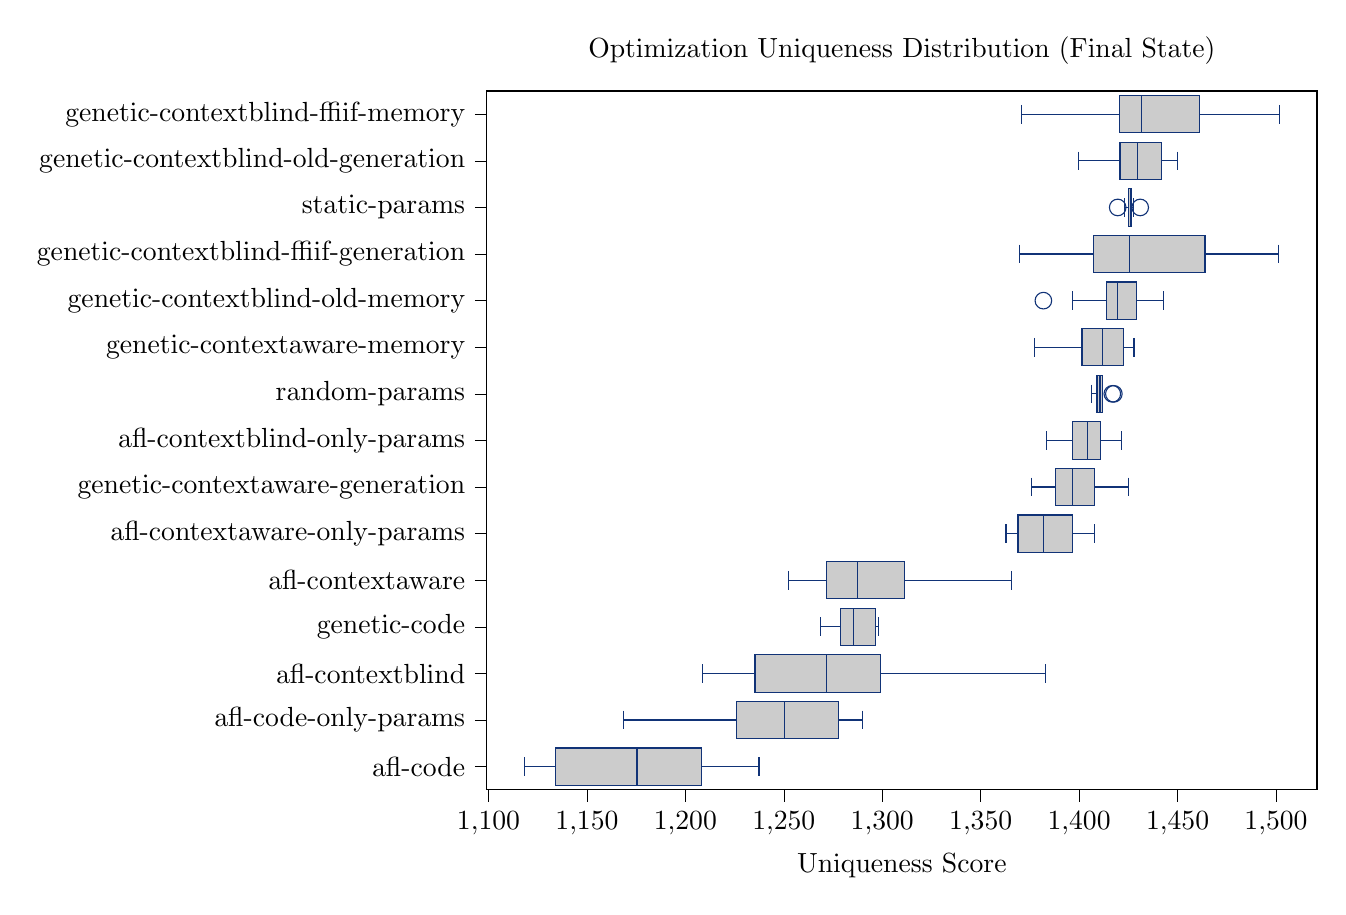
\begin{tikzpicture}

\definecolor{darkgray176}{RGB}{176,176,176}
\definecolor{lightgray204}{RGB}{204,204,204}
\definecolor{midnightblue1751119}{RGB}{17,51,119}

\begin{axis}[
tick align=outside,
tick pos=left,
title={Optimization Uniqueness Distribution (Final State)},
width=\linewidth,
x grid style={darkgray176},
xlabel={Uniqueness Score},
xmin=1099.10946643277, xmax=1520.79900348627,
xtick style={color=black},
y dir=reverse,
y grid style={darkgray176},
ymin=-0.5, ymax=14.5,
ytick style={color=black},
ytick={0,1,2,3,4,5,6,7,8,9,10,11,12,13,14},
yticklabels={
  genetic-contextblind-ffiif-memory,
  genetic-contextblind-old-generation,
  static-params,
  genetic-contextblind-ffiif-generation,
  genetic-contextblind-old-memory,
  genetic-contextaware-memory,
  random-params,
  afl-contextblind-only-params,
  genetic-contextaware-generation,
  afl-contextaware-only-params,
  afl-contextaware,
  genetic-code,
  afl-contextblind,
  afl-code-only-params,
  afl-code
}
]
\path [draw=midnightblue1751119, fill=lightgray204]
(axis cs:1420.65370430417,-0.4)
--(axis cs:1420.65370430417,0.4)
--(axis cs:1461.0904592425,0.4)
--(axis cs:1461.0904592425,-0.4)
--(axis cs:1420.65370430417,-0.4)
--cycle;
\addplot [midnightblue1751119]
table {%
1420.65370430417 0
1370.80028216035 0
};
\addplot [midnightblue1751119]
table {%
1461.0904592425 0
1501.63129725657 0
};
\addplot [midnightblue1751119]
table {%
1370.80028216035 -0.2
1370.80028216035 0.2
};
\addplot [midnightblue1751119]
table {%
1501.63129725657 -0.2
1501.63129725657 0.2
};
\path [draw=midnightblue1751119, fill=lightgray204]
(axis cs:1420.7585152318,0.6)
--(axis cs:1420.7585152318,1.4)
--(axis cs:1441.62081620477,1.4)
--(axis cs:1441.62081620477,0.6)
--(axis cs:1420.7585152318,0.6)
--cycle;
\addplot [midnightblue1751119]
table {%
1420.7585152318 1
1399.53500513717 1
};
\addplot [midnightblue1751119]
table {%
1441.62081620477 1
1449.76119113495 1
};
\addplot [midnightblue1751119]
table {%
1399.53500513717 0.8
1399.53500513717 1.2
};
\addplot [midnightblue1751119]
table {%
1449.76119113495 0.8
1449.76119113495 1.2
};
\path [draw=midnightblue1751119, fill=lightgray204]
(axis cs:1424.96472601644,1.6)
--(axis cs:1424.96472601644,2.4)
--(axis cs:1426.58133777807,2.4)
--(axis cs:1426.58133777807,1.6)
--(axis cs:1424.96472601644,1.6)
--cycle;
\addplot [midnightblue1751119]
table {%
1424.96472601644 2
1423.16290710207 2
};
\addplot [midnightblue1751119]
table {%
1426.58133777807 2
1427.4581410835 2
};
\addplot [midnightblue1751119]
table {%
1423.16290710207 1.8
1423.16290710207 2.2
};
\addplot [midnightblue1751119]
table {%
1427.4581410835 1.8
1427.4581410835 2.2
};
\addplot [black, mark=o, mark size=3, mark options={solid,fill opacity=0,draw=midnightblue1751119}, only marks]
table {%
1419.59590843234 2
1431.01212913747 2
};
\path [draw=midnightblue1751119, fill=lightgray204]
(axis cs:1407.12261289619,2.6)
--(axis cs:1407.12261289619,3.4)
--(axis cs:1463.93139298699,3.4)
--(axis cs:1463.93139298699,2.6)
--(axis cs:1407.12261289619,2.6)
--cycle;
\addplot [midnightblue1751119]
table {%
1407.12261289619 3
1369.9320181696 3
};
\addplot [midnightblue1751119]
table {%
1463.93139298699 3
1501.23108711934 3
};
\addplot [midnightblue1751119]
table {%
1369.9320181696 2.8
1369.9320181696 3.2
};
\addplot [midnightblue1751119]
table {%
1501.23108711934 2.8
1501.23108711934 3.2
};
\path [draw=midnightblue1751119, fill=lightgray204]
(axis cs:1413.80732375024,3.6)
--(axis cs:1413.80732375024,4.4)
--(axis cs:1428.90613047095,4.4)
--(axis cs:1428.90613047095,3.6)
--(axis cs:1413.80732375024,3.6)
--cycle;
\addplot [midnightblue1751119]
table {%
1413.80732375024 4
1396.80973258614 4
};
\addplot [midnightblue1751119]
table {%
1428.90613047095 4
1442.65570336829 4
};
\addplot [midnightblue1751119]
table {%
1396.80973258614 3.8
1396.80973258614 4.2
};
\addplot [midnightblue1751119]
table {%
1442.65570336829 3.8
1442.65570336829 4.2
};
\addplot [black, mark=o, mark size=3, mark options={solid,fill opacity=0,draw=midnightblue1751119}, only marks]
table {%
1381.8384508219 4
};
\path [draw=midnightblue1751119, fill=lightgray204]
(axis cs:1401.42802623561,4.6)
--(axis cs:1401.42802623561,5.4)
--(axis cs:1422.73818376056,5.4)
--(axis cs:1422.73818376056,4.6)
--(axis cs:1401.42802623561,4.6)
--cycle;
\addplot [midnightblue1751119]
table {%
1401.42802623561 5
1377.42275555384 5
};
\addplot [midnightblue1751119]
table {%
1422.73818376056 5
1427.84182304711 5
};
\addplot [midnightblue1751119]
table {%
1377.42275555384 4.8
1377.42275555384 5.2
};
\addplot [midnightblue1751119]
table {%
1427.84182304711 4.8
1427.84182304711 5.2
};
\path [draw=midnightblue1751119, fill=lightgray204]
(axis cs:1409.09661151059,5.6)
--(axis cs:1409.09661151059,6.4)
--(axis cs:1411.76718086367,6.4)
--(axis cs:1411.76718086367,5.6)
--(axis cs:1409.09661151059,5.6)
--cycle;
\addplot [midnightblue1751119]
table {%
1409.09661151059 6
1406.1400597094 6
};
\addplot [midnightblue1751119]
table {%
1411.76718086367 6
1411.77017154179 6
};
\addplot [midnightblue1751119]
table {%
1406.1400597094 5.8
1406.1400597094 6.2
};
\addplot [midnightblue1751119]
table {%
1411.77017154179 5.8
1411.77017154179 6.2
};
\addplot [black, mark=o, mark size=3, mark options={solid,fill opacity=0,draw=midnightblue1751119}, only marks]
table {%
1417.63253866532 6
1416.84771851669 6
};
\path [draw=midnightblue1751119, fill=lightgray204]
(axis cs:1396.42833766223,6.6)
--(axis cs:1396.42833766223,7.4)
--(axis cs:1410.89134932837,7.4)
--(axis cs:1410.89134932837,6.6)
--(axis cs:1396.42833766223,6.6)
--cycle;
\addplot [midnightblue1751119]
table {%
1396.42833766223 7
1383.36651440937 7
};
\addplot [midnightblue1751119]
table {%
1410.89134932837 7
1421.45836302164 7
};
\addplot [midnightblue1751119]
table {%
1383.36651440937 6.8
1383.36651440937 7.2
};
\addplot [midnightblue1751119]
table {%
1421.45836302164 6.8
1421.45836302164 7.2
};
\path [draw=midnightblue1751119, fill=lightgray204]
(axis cs:1387.90490299268,7.6)
--(axis cs:1387.90490299268,8.4)
--(axis cs:1407.7154734784,8.4)
--(axis cs:1407.7154734784,7.6)
--(axis cs:1387.90490299268,7.6)
--cycle;
\addplot [midnightblue1751119]
table {%
1387.90490299268 8
1375.71871425944 8
};
\addplot [midnightblue1751119]
table {%
1407.7154734784 8
1424.93063259519 8
};
\addplot [midnightblue1751119]
table {%
1375.71871425944 7.8
1375.71871425944 8.2
};
\addplot [midnightblue1751119]
table {%
1424.93063259519 7.8
1424.93063259519 8.2
};
\path [draw=midnightblue1751119, fill=lightgray204]
(axis cs:1368.92532025992,8.6)
--(axis cs:1368.92532025992,9.4)
--(axis cs:1396.76251404772,9.4)
--(axis cs:1396.76251404772,8.6)
--(axis cs:1368.92532025992,8.6)
--cycle;
\addplot [midnightblue1751119]
table {%
1368.92532025992 9
1362.84257487455 9
};
\addplot [midnightblue1751119]
table {%
1396.76251404772 9
1407.65763804731 9
};
\addplot [midnightblue1751119]
table {%
1362.84257487455 8.8
1362.84257487455 9.2
};
\addplot [midnightblue1751119]
table {%
1407.65763804731 8.8
1407.65763804731 9.2
};
\path [draw=midnightblue1751119, fill=lightgray204]
(axis cs:1271.79689068658,9.6)
--(axis cs:1271.79689068658,10.4)
--(axis cs:1311.36131435135,10.4)
--(axis cs:1311.36131435135,9.6)
--(axis cs:1271.79689068658,9.6)
--cycle;
\addplot [midnightblue1751119]
table {%
1271.79689068658 10
1252.42167474449 10
};
\addplot [midnightblue1751119]
table {%
1311.36131435135 10
1365.41748868479 10
};
\addplot [midnightblue1751119]
table {%
1252.42167474449 9.8
1252.42167474449 10.2
};
\addplot [midnightblue1751119]
table {%
1365.41748868479 9.8
1365.41748868479 10.2
};
\path [draw=midnightblue1751119, fill=lightgray204]
(axis cs:1278.80202215791,10.6)
--(axis cs:1278.80202215791,11.4)
--(axis cs:1296.37705431289,11.4)
--(axis cs:1296.37705431289,10.6)
--(axis cs:1278.80202215791,10.6)
--cycle;
\addplot [midnightblue1751119]
table {%
1278.80202215791 11
1268.68576163016 11
};
\addplot [midnightblue1751119]
table {%
1296.37705431289 11
1298.03043245592 11
};
\addplot [midnightblue1751119]
table {%
1268.68576163016 10.8
1268.68576163016 11.2
};
\addplot [midnightblue1751119]
table {%
1298.03043245592 10.8
1298.03043245592 11.2
};
\path [draw=midnightblue1751119, fill=lightgray204]
(axis cs:1235.3517960264,11.6)
--(axis cs:1235.3517960264,12.4)
--(axis cs:1299.30719106888,12.4)
--(axis cs:1299.30719106888,11.6)
--(axis cs:1235.3517960264,11.6)
--cycle;
\addplot [midnightblue1751119]
table {%
1235.3517960264 12
1208.6166726443 12
};
\addplot [midnightblue1751119]
table {%
1299.30719106888 12
1382.97070315399 12
};
\addplot [midnightblue1751119]
table {%
1208.6166726443 11.8
1208.6166726443 12.2
};
\addplot [midnightblue1751119]
table {%
1382.97070315399 11.8
1382.97070315399 12.2
};
\path [draw=midnightblue1751119, fill=lightgray204]
(axis cs:1225.88076229124,12.6)
--(axis cs:1225.88076229124,13.4)
--(axis cs:1277.97894766275,13.4)
--(axis cs:1277.97894766275,12.6)
--(axis cs:1225.88076229124,12.6)
--cycle;
\addplot [midnightblue1751119]
table {%
1225.88076229124 13
1168.51637752774 13
};
\addplot [midnightblue1751119]
table {%
1277.97894766275 13
1290.01713226872 13
};
\addplot [midnightblue1751119]
table {%
1168.51637752774 12.8
1168.51637752774 13.2
};
\addplot [midnightblue1751119]
table {%
1290.01713226872 12.8
1290.01713226872 13.2
};
\path [draw=midnightblue1751119, fill=lightgray204]
(axis cs:1134.09932967528,13.6)
--(axis cs:1134.09932967528,14.4)
--(axis cs:1207.97745942132,14.4)
--(axis cs:1207.97745942132,13.6)
--(axis cs:1134.09932967528,13.6)
--cycle;
\addplot [midnightblue1751119]
table {%
1134.09932967528 14
1118.27717266247 14
};
\addplot [midnightblue1751119]
table {%
1207.97745942132 14
1237.38163034107 14
};
\addplot [midnightblue1751119]
table {%
1118.27717266247 13.8
1118.27717266247 14.2
};
\addplot [midnightblue1751119]
table {%
1237.38163034107 13.8
1237.38163034107 14.2
};
\addplot [midnightblue1751119]
table {%
1431.69631402081 -0.4
1431.69631402081 0.4
};
\addplot [midnightblue1751119]
table {%
1429.59180750733 0.6
1429.59180750733 1.4
};
\addplot [midnightblue1751119]
table {%
1426.25127288117 1.6
1426.25127288117 2.4
};
\addplot [midnightblue1751119]
table {%
1425.56073140991 2.6
1425.56073140991 3.4
};
\addplot [midnightblue1751119]
table {%
1419.25888949408 3.6
1419.25888949408 4.4
};
\addplot [midnightblue1751119]
table {%
1411.71321082972 4.6
1411.71321082972 5.4
};
\addplot [midnightblue1751119]
table {%
1410.61947547669 5.6
1410.61947547669 6.4
};
\addplot [midnightblue1751119]
table {%
1404.38663605407 6.6
1404.38663605407 7.4
};
\addplot [midnightblue1751119]
table {%
1396.73141369904 7.6
1396.73141369904 8.4
};
\addplot [midnightblue1751119]
table {%
1382.05754898943 8.6
1382.05754898943 9.4
};
\addplot [midnightblue1751119]
table {%
1287.31395316225 9.6
1287.31395316225 10.4
};
\addplot [midnightblue1751119]
table {%
1285.45923206501 10.6
1285.45923206501 11.4
};
\addplot [midnightblue1751119]
table {%
1271.53462794507 11.6
1271.53462794507 12.4
};
\addplot [midnightblue1751119]
table {%
1250.23660234985 12.6
1250.23660234985 13.4
};
\addplot [midnightblue1751119]
table {%
1175.42564949101 13.6
1175.42564949101 14.4
};
\end{axis}

\end{tikzpicture}
%
    \endgroup
    \caption{Uniqueness scores of different configurations (and variants) based on triggered rare optimizations.
    \label{fig:rare-opts}
    See \cref{ss:eval-rare-opts} for details.}
\end{figure}

\begin{figure}[t]
    \centering
    \begingroup
    \pgfplotsset{
        every axis/.append style={
            yticklabel style={font=\propernamedecl\footnotesize},
            execute at begin axis={
                \pgfplotsset{title={Optimization Pair Uniqueness after 24h},
                    width=0.75\textwidth,
                    height=0.7\linewidth}
            },
        },
    }
    % This file was created with matplot2tikz v0.4.0.
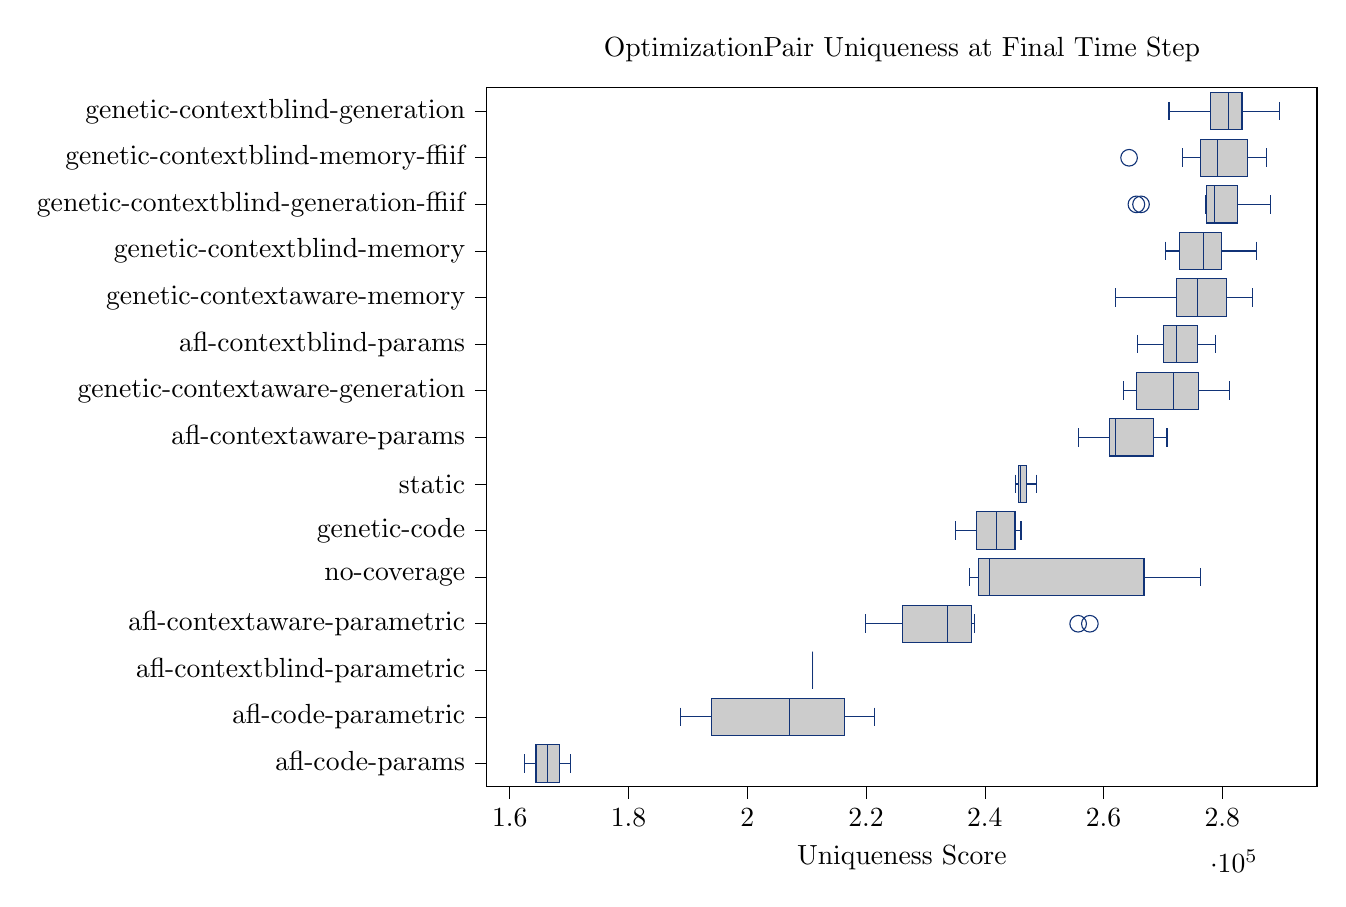
\begin{tikzpicture}

\definecolor{darkgray176}{RGB}{176,176,176}
\definecolor{lightgray204}{RGB}{204,204,204}
\definecolor{midnightblue1751119}{RGB}{17,51,119}

\begin{axis}[
tick align=outside,
tick pos=left,
title={OptimizationPair Uniqueness at Final Time Step},
width=\linewidth,
x grid style={darkgray176},
xlabel={Uniqueness Score},
xmin=156120.909333459, xmax=295943.441329031,
xtick style={color=black},
y dir=reverse,
y grid style={darkgray176},
ymin=-0.5, ymax=14.5,
ytick style={color=black},
ytick={0,1,2,3,4,5,6,7,8,9,10,11,12,13,14},
yticklabels={
  genetic-contextblind-generation,
  genetic-contextblind-memory-ffiif,
  genetic-contextblind-generation-ffiif,
  genetic-contextblind-memory,
  genetic-contextaware-memory,
  afl-contextblind-params,
  genetic-contextaware-generation,
  afl-contextaware-params,
  static,
  genetic-code,
  no-coverage,
  afl-contextaware-parametric,
  afl-contextblind-parametric,
  afl-code-parametric,
  afl-code-params
}
]
\path [draw=midnightblue1751119, fill=lightgray204]
(axis cs:277953.440212219,-0.4)
--(axis cs:277953.440212219,0.4)
--(axis cs:283315.846064258,0.4)
--(axis cs:283315.846064258,-0.4)
--(axis cs:277953.440212219,-0.4)
--cycle;
\addplot [midnightblue1751119]
table {%
277953.440212219 0
271030.361656792 0
};
\addplot [midnightblue1751119]
table {%
283315.846064258 0
289587.871692869 0
};
\addplot [midnightblue1751119]
table {%
271030.361656792 -0.2
271030.361656792 0.2
};
\addplot [midnightblue1751119]
table {%
289587.871692869 -0.2
289587.871692869 0.2
};
\path [draw=midnightblue1751119, fill=lightgray204]
(axis cs:276321.450477075,0.6)
--(axis cs:276321.450477075,1.4)
--(axis cs:284223.966778089,1.4)
--(axis cs:284223.966778089,0.6)
--(axis cs:276321.450477075,0.6)
--cycle;
\addplot [midnightblue1751119]
table {%
276321.450477075 1
273228.864873659 1
};
\addplot [midnightblue1751119]
table {%
284223.966778089 1
287500.8122168 1
};
\addplot [midnightblue1751119]
table {%
273228.864873659 0.8
273228.864873659 1.2
};
\addplot [midnightblue1751119]
table {%
287500.8122168 0.8
287500.8122168 1.2
};
\addplot [black, mark=o, mark size=3, mark options={solid,fill opacity=0,draw=midnightblue1751119}, only marks]
table {%
264299.494248465 1
};
\path [draw=midnightblue1751119, fill=lightgray204]
(axis cs:277319.142230507,1.6)
--(axis cs:277319.142230507,2.4)
--(axis cs:282626.637877005,2.4)
--(axis cs:282626.637877005,1.6)
--(axis cs:277319.142230507,1.6)
--cycle;
\addplot [midnightblue1751119]
table {%
277319.142230507 2
277179.393731311 2
};
\addplot [midnightblue1751119]
table {%
282626.637877005 2
288081.007370516 2
};
\addplot [midnightblue1751119]
table {%
277179.393731311 1.8
277179.393731311 2.2
};
\addplot [midnightblue1751119]
table {%
288081.007370516 1.8
288081.007370516 2.2
};
\addplot [black, mark=o, mark size=3, mark options={solid,fill opacity=0,draw=midnightblue1751119}, only marks]
table {%
266312.410583593 2
265533.361534734 2
};
\path [draw=midnightblue1751119, fill=lightgray204]
(axis cs:272745.983909547,2.6)
--(axis cs:272745.983909547,3.4)
--(axis cs:279910.873919318,3.4)
--(axis cs:279910.873919318,2.6)
--(axis cs:272745.983909547,2.6)
--cycle;
\addplot [midnightblue1751119]
table {%
272745.983909547 3
270428.785759479 3
};
\addplot [midnightblue1751119]
table {%
279910.873919318 3
285789.991942737 3
};
\addplot [midnightblue1751119]
table {%
270428.785759479 2.8
270428.785759479 3.2
};
\addplot [midnightblue1751119]
table {%
285789.991942737 2.8
285789.991942737 3.2
};
\path [draw=midnightblue1751119, fill=lightgray204]
(axis cs:272242.369144191,3.6)
--(axis cs:272242.369144191,4.4)
--(axis cs:280719.896229137,4.4)
--(axis cs:280719.896229137,3.6)
--(axis cs:272242.369144191,3.6)
--cycle;
\addplot [midnightblue1751119]
table {%
272242.369144191 4
261953.664031869 4
};
\addplot [midnightblue1751119]
table {%
280719.896229137 4
285093.423611437 4
};
\addplot [midnightblue1751119]
table {%
261953.664031869 3.8
261953.664031869 4.2
};
\addplot [midnightblue1751119]
table {%
285093.423611437 3.8
285093.423611437 4.2
};
\path [draw=midnightblue1751119, fill=lightgray204]
(axis cs:270081.277302514,4.6)
--(axis cs:270081.277302514,5.4)
--(axis cs:275884.144553685,5.4)
--(axis cs:275884.144553685,4.6)
--(axis cs:270081.277302514,4.6)
--cycle;
\addplot [midnightblue1751119]
table {%
270081.277302514 5
265717.47506831 5
};
\addplot [midnightblue1751119]
table {%
275884.144553685 5
278912.194976947 5
};
\addplot [midnightblue1751119]
table {%
265717.47506831 4.8
265717.47506831 5.2
};
\addplot [midnightblue1751119]
table {%
278912.194976947 4.8
278912.194976947 5.2
};
\path [draw=midnightblue1751119, fill=lightgray204]
(axis cs:265530.544856777,5.6)
--(axis cs:265530.544856777,6.4)
--(axis cs:275921.235648894,6.4)
--(axis cs:275921.235648894,5.6)
--(axis cs:265530.544856777,5.6)
--cycle;
\addplot [midnightblue1751119]
table {%
265530.544856777 6
263426.390826741 6
};
\addplot [midnightblue1751119]
table {%
275921.235648894 6
281180.182736596 6
};
\addplot [midnightblue1751119]
table {%
263426.390826741 5.8
263426.390826741 6.2
};
\addplot [midnightblue1751119]
table {%
281180.182736596 5.8
281180.182736596 6.2
};
\path [draw=midnightblue1751119, fill=lightgray204]
(axis cs:260987.75900005,6.6)
--(axis cs:260987.75900005,7.4)
--(axis cs:268397.679125152,7.4)
--(axis cs:268397.679125152,6.6)
--(axis cs:260987.75900005,6.6)
--cycle;
\addplot [midnightblue1751119]
table {%
260987.75900005 7
255842.604688313 7
};
\addplot [midnightblue1751119]
table {%
268397.679125152 7
270686.664141726 7
};
\addplot [midnightblue1751119]
table {%
255842.604688313 6.8
255842.604688313 7.2
};
\addplot [midnightblue1751119]
table {%
270686.664141726 6.8
270686.664141726 7.2
};
\path [draw=midnightblue1751119, fill=lightgray204]
(axis cs:245710.451474509,7.6)
--(axis cs:245710.451474509,8.4)
--(axis cs:247064.132193546,8.4)
--(axis cs:247064.132193546,7.6)
--(axis cs:245710.451474509,7.6)
--cycle;
\addplot [midnightblue1751119]
table {%
245710.451474509 8
245115.571542708 8
};
\addplot [midnightblue1751119]
table {%
247064.132193546 8
248703.81213221 8
};
\addplot [midnightblue1751119]
table {%
245115.571542708 7.8
245115.571542708 8.2
};
\addplot [midnightblue1751119]
table {%
248703.81213221 7.8
248703.81213221 8.2
};
\path [draw=midnightblue1751119, fill=lightgray204]
(axis cs:238623.700293406,8.6)
--(axis cs:238623.700293406,9.4)
--(axis cs:245080.272090991,9.4)
--(axis cs:245080.272090991,8.6)
--(axis cs:238623.700293406,8.6)
--cycle;
\addplot [midnightblue1751119]
table {%
238623.700293406 9
235074.155260022 9
};
\addplot [midnightblue1751119]
table {%
245080.272090991 9
246090.619086918 9
};
\addplot [midnightblue1751119]
table {%
235074.155260022 8.8
235074.155260022 9.2
};
\addplot [midnightblue1751119]
table {%
246090.619086918 8.8
246090.619086918 9.2
};
\path [draw=midnightblue1751119, fill=lightgray204]
(axis cs:239009.293847989,9.6)
--(axis cs:239009.293847989,10.4)
--(axis cs:266811.79701274,10.4)
--(axis cs:266811.79701274,9.6)
--(axis cs:239009.293847989,9.6)
--cycle;
\addplot [midnightblue1751119]
table {%
239009.293847989 10
237428.122246795 10
};
\addplot [midnightblue1751119]
table {%
266811.79701274 10
276330.540146626 10
};
\addplot [midnightblue1751119]
table {%
237428.122246795 9.8
237428.122246795 10.2
};
\addplot [midnightblue1751119]
table {%
276330.540146626 9.8
276330.540146626 10.2
};
\path [draw=midnightblue1751119, fill=lightgray204]
(axis cs:226197.261310072,10.6)
--(axis cs:226197.261310072,11.4)
--(axis cs:237803.38032637,11.4)
--(axis cs:237803.38032637,10.6)
--(axis cs:226197.261310072,10.6)
--cycle;
\addplot [midnightblue1751119]
table {%
226197.261310072 11
219846.467137529 11
};
\addplot [midnightblue1751119]
table {%
237803.38032637 11
238324.704512253 11
};
\addplot [midnightblue1751119]
table {%
219846.467137529 10.8
219846.467137529 11.2
};
\addplot [midnightblue1751119]
table {%
238324.704512253 10.8
238324.704512253 11.2
};
\addplot [black, mark=o, mark size=3, mark options={solid,fill opacity=0,draw=midnightblue1751119}, only marks]
table {%
255720.264480067 11
257695.031778287 11
};
\path [draw=midnightblue1751119, fill=lightgray204]
(axis cs:211033.329712607,11.6)
--(axis cs:211033.329712607,12.4)
--(axis cs:211033.329712607,12.4)
--(axis cs:211033.329712607,11.6)
--(axis cs:211033.329712607,11.6)
--cycle;
\addplot [midnightblue1751119]
table {%
211033.329712607 12
211033.329712607 12
};
\addplot [midnightblue1751119]
table {%
211033.329712607 12
211033.329712607 12
};
\addplot [midnightblue1751119]
table {%
211033.329712607 11.8
211033.329712607 12.2
};
\addplot [midnightblue1751119]
table {%
211033.329712607 11.8
211033.329712607 12.2
};
\path [draw=midnightblue1751119, fill=lightgray204]
(axis cs:193986.829759283,12.6)
--(axis cs:193986.829759283,13.4)
--(axis cs:216309.391668908,13.4)
--(axis cs:216309.391668908,12.6)
--(axis cs:193986.829759283,12.6)
--cycle;
\addplot [midnightblue1751119]
table {%
193986.829759283 13
188729.334355677 13
};
\addplot [midnightblue1751119]
table {%
216309.391668908 13
221452.703553717 13
};
\addplot [midnightblue1751119]
table {%
188729.334355677 12.8
188729.334355677 13.2
};
\addplot [midnightblue1751119]
table {%
221452.703553717 12.8
221452.703553717 13.2
};
\path [draw=midnightblue1751119, fill=lightgray204]
(axis cs:164420.581305993,13.6)
--(axis cs:164420.581305993,14.4)
--(axis cs:168308.785978736,14.4)
--(axis cs:168308.785978736,13.6)
--(axis cs:164420.581305993,13.6)
--cycle;
\addplot [midnightblue1751119]
table {%
164420.581305993 14
162476.478969621 14
};
\addplot [midnightblue1751119]
table {%
168308.785978736 14
170252.888315108 14
};
\addplot [midnightblue1751119]
table {%
162476.478969621 13.8
162476.478969621 14.2
};
\addplot [midnightblue1751119]
table {%
170252.888315108 13.8
170252.888315108 14.2
};
\addplot [midnightblue1751119]
table {%
280993.164952848 -0.4
280993.164952848 0.4
};
\addplot [midnightblue1751119]
table {%
279147.755892618 0.6
279147.755892618 1.4
};
\addplot [midnightblue1751119]
table {%
278738.741742052 1.6
278738.741742052 2.4
};
\addplot [midnightblue1751119]
table {%
276873.777026243 2.6
276873.777026243 3.4
};
\addplot [midnightblue1751119]
table {%
275895.950865476 3.6
275895.950865476 4.4
};
\addplot [midnightblue1751119]
table {%
272250.194229867 4.6
272250.194229867 5.4
};
\addplot [midnightblue1751119]
table {%
271706.921457256 5.6
271706.921457256 6.4
};
\addplot [midnightblue1751119]
table {%
262080.771506874 6.6
262080.771506874 7.4
};
\addplot [midnightblue1751119]
table {%
246010.571791481 7.6
246010.571791481 8.4
};
\addplot [midnightblue1751119]
table {%
241953.518655476 8.6
241953.518655476 9.4
};
\addplot [midnightblue1751119]
table {%
240854.54972975 9.6
240854.54972975 10.4
};
\addplot [midnightblue1751119]
table {%
233767.109931736 10.6
233767.109931736 11.4
};
\addplot [midnightblue1751119]
table {%
211033.329712607 11.6
211033.329712607 12.4
};
\addplot [midnightblue1751119]
table {%
207151.024234722 12.6
207151.024234722 13.4
};
\addplot [midnightblue1751119]
table {%
166364.683642365 13.6
166364.683642365 14.4
};
\end{axis}

\end{tikzpicture}
%
    \endgroup
    \caption{Uniqueness scores of different configurations (and variants) based on triggered rare optimization pairs.
    \label{fig:rare-pairs}
    See \cref{ss:eval-rare-opts} for details.}
\end{figure}


We evaluated both the rareness of single optimizations and the rareness of optimization pairs.
In the following text, we use \emph{feature} to mean either optimizations or optimization pairs.

We define the \enquote{rareness} $R(f)$ of a particular feature $f \in F$ as
\[ R(f) = \log\left( \frac{\sum_{f_j \in F}{\mathrm{count}(f_j)}}{\mathrm{count}(f)} \right) \]
where $\mathrm{count}(f)$ is the number of occurrences of $f$ across \emph{all} experiments.
That is, the less often a feature occurred in \emph{any} experiment, the rarer it is.
We only consider features that occurred at least once overall.
The logarithm scales down extremely common features, such as the \propername{CanonicalReplacement} optimization.
We found that due to the very high counts of these features, they would disproportionately contribute to an experiment's overall score, despite being so common.

Based on this definition we calculate a score for each run in a configuration that rates how many rare optimizations or optimization pairs the configuration triggered.
The score for a run is simply the sum of all individual feature scores in that run.
The boxplots in \cref{fig:rare-opts,fig:rare-pairs} illustrate statistics based on the rareness scores of the runs in a configuration.
The boxplot in \cref{fig:rare-opts} is based on optimization rareness scores and the boxplot in \cref{fig:rare-pairs} is based on optimization-pair rareness scores.
Note that the scores for optimizations and optimization pairs are not directly comparable.

\section{Discussion}\label{s:discussion}

\newcommand{\rpairvsmaxcorrelation}{\ensuremath{0.9505016978980805}}
\newcommand{\regressionr}{\ensuremath{0.8841179762377677}}
\newcommand{\pmimean}{\ensuremath{0.11721308111143029}}
\newcommand{\experimentrankcorrelation}{\ensuremath{0.9824175824175824}}


\subsection{Coverage vs. No Coverage}
The main advantage of having no coverage at all is the higher execution speed, as evidenced by the data in \cref{tbl:coverage-overhead}.
On the other hand, coverage feedback enables guidance through feedback-directed input mutation.
\cref{fig:cumulative-coverage} shows that \propername{random-params}, \ie without feedback but with random generation parameters, achieves the highest cumulative code coverage of all configurations.
This advantage in code coverage is not, however, reflected in the achieved rare optimization scores (see \cref{fig:rare-opts,fig:rare-pairs}).
\propername{Random-params} ranks below all of the feedback-driven configurations based on the genetic algorithm.
One possible explanation is that even if \propername{random-params} discovers new code coverage, the lack of feedback means the configuration cannot build on these gains systematically.
Unlike rare optimization scores, cumulative code coverage does not reflect how consistently a configuration triggers edges.
A single lucky test can boost the cumulative coverage of an entire run.
Although \propername{random-params} is more stable in terms of triggering rare optimizations, its best run is only as good as the weakest quartile of the feedback-driven runs.
\propername{Static-params} on the other hand achieves less code coverage than the feedback-driven configurations, but reaches high rare optimization scores.
The high scores are likely the result of the manual tuning that went into the \propername{static-params} configuration over the last years, with the explicit goal of triggering interesting optimizations.

Despite the lack of feedback, both \propername{random-params} and \propername{static-params} achieve better results than \aflpp-based configurations.
We attribute the improvement of the unguided configurations over \aflpp to the more structural issues with \aflpp, which we discuss in \cref{ss:aflpp-vs-genetic}.

\begin{infobox}
    \textbf{\ref{hpt:feedback-vs-nofeedback}}\hspace{0.8em}\ding{51}
    While coverage feedback does not lead to higher cumulative code coverage compared to \propername{random-params}, the feedback enables higher optimization rareness scores.
    Configurations based on the genetic algorithm achieve higher rareness scores than \propername{random-params} and also slightly higher scores than \propername{static-params}.

\end{infobox}

\subsection{\aflpp vs. Genetic Parameter Mutation}\label{ss:aflpp-vs-genetic}
\begin{table}[!t]
    \small
    \caption{The number of identical test runs and how many tests were successfully generated on the first try or had to be retried with reduced generation parameters.}
    \label{tbl:afl-overview}
    \begin{tabular}{>{\nextrow}E C C C C C C C C C}
        \toprule
        \multicolumn{4}{c}{} & \multicolumn{6}{c}{Attempts} \\
        \cmidrule(lr){5-10}
        {Experiment} & {Total} & {Skipped} & {Identical} & {First} & {Once} & {Second} & {Third} & {Fourth} & {Fifth} \\
        \midrule
        \fileInput{generated/lool/afl-test-overview}
        \bottomrule
    \end{tabular}

\end{table}


The cumulative coverage in \cref{fig:cumulative-coverage} indicates that our custom genetic algorithm outperforms the \aflpp and \propername{static-params} configurations in terms of code coverage.
The only exception is \propername{genetic-code}, which achieves less code coverage than the \propername{static-params} and the \propername{random-params} configuration.
We attribute this difference to the significantly reduced test throughput of \propername{genetic-code}, caused by the code coverage instrumentation.
\cref{fig:rare-opts,fig:rare-pairs} show that \propername{genetic-code} nonetheless triggers a similar amount of rare optimizations and pairs.

Except for the \propername{afl-contextblind-only-params} configuration, all \aflpp-based configurations achieve less coverage than even the \propername{static-params} configuration.
One reason for \aflpp's poor performance lies in the translation of \aflpp generated input files to generated test cases.
We found that over stretches of dozens of generated tests the \aflpp configurations generate either \emph{identical} tests or \emph{small tests}, which are the result of re-generation attempts.
The number of identical tests and re-generation attempts are shown in \cref{tbl:afl-overview}.

Identical tests happen when \aflpp mutates bits in the input file that do not change the code generator's behavior.
Although \aflpp eventually learns that mutating these bits is useless, the feedback loop in the GraalVM context is slow compared to traditional \aflpp targets such as image libraries.
On average, a generated test case takes 9--10s, which means that \aflpp often wastes several minutes trying to mutate meaningless bits.
In the variants that mutate only generation parameters (see \cref{sss:afl-hyperonly}), the generator reads a short, fixed byte sequence from the \aflpp generated input, making it easier for \aflpp to detect which bits have an effect.
Nonetheless, even though we started with an ideally sized seed file, \aflpp eventually tries different sizes as well and wastes time with meaningless mutations.
Another source of identical tests are \aflpp calibration runs, which become particularly expensive with long-running tests.
The problem is compounded by the fact that neither the coverage feedback nor the execution times are fully stable, due to the JVM's profiling and class-loading heuristics.
\cref{tbl:afl-overview} shows the number of identical tests summed over all runs of an experiment for each of the \aflpp configurations.

Small tests happen when \aflpp generates input files that are too small for the generator to generate valid test cases.
Again, this is more likely to happen in the fully parametric case because there, earlier bits in the file can change how many more random bits are needed later on.
This variable length requirement makes it difficult for \aflpp to infer useful file sizes.
In cases where there is too little randomness for the generator's random decisions, the generator tries to size down the generated test case by adapting structural parameters (see \cref{sss:afl-fully-parametric}).
We found that in the fully parametric variant (see \cref{sss:afl-fully-parametric}) the generator reduced the parameters of almost all tests at least once.
\cref{tbl:afl-overview} shows the number of tests with reduced generation parameters for each configuration.
As expected, this effect is mitigated in the variant that reads only generation parameters from the seed (see \cref{sss:afl-hyperonly}).
In this variant, the generator fails only if the seed is even too short to read generation parameters, which happened in about 5\% of the generated tests.
The \enquote{Skipped} column in \cref{tbl:test-overview} shows the number of tests that had to be skipped due to such an unusable seed file.

The difference between \propername{afl-contextblind-only-params} and the other \aflpp based configurations can be explained by looking at \aflpp's statistics.
Apart from the slowdown caused by code coverage, the primary slowdown for \aflpp configurations is the calibration and trimming time.
The code coverage and context-aware \aflpp configurations spent only between 10\% and 20\% of the total runtime actually fuzzing, the rest of the time was calibration and trimming.
Paradoxically, \propername{afl-contextblind} and \propername{afl-contextblind-only-params} are less affected by trimming because \aflpp sees their coverage as \emph{less} stable.
The mapping of global optimization counters to \aflpp's coverage bitmap occupies only about 80 bytes, leading to large relative changes if even only one counter changes.
The code coverage and context-aware coverage types occupy larger parts of the bitmap and lead to higher stability.
Unstable seeds are not further calibrated, thus avoiding the enormous overhead caused by calibrating slow running seeds.
This difference is reflected in the low calibration times of 2\% and 4\% of the total runtime in \propername{afl-globalcounters} and \propername{afl-globalcounters-hyperonly}.
\propername{afl-globalcounter} loses this advantage again, however, by spending 90\% of the total runtime in trimming.

Configurations using the genetic algorithm consistently trigger more rare optimizations and optimization pairs than their \aflpp counterparts (see \cref{fig:rare-opts,fig:rare-pairs}).
For example, \propername{genetic-code} achieves a higher rareness score than \propername{afl-code-only-params} and \propername{afl-code}.
The domain-specific mutation has the advantage of knowing the types of the mutated parameters and is thus able to mutate them in small incremental steps.

Some of the issues described above could be mitigated with \aflpp options, but nonetheless \aflpp's learning process through rapid iteration is hampered by long running tests.
Overall, \aflpp's heuristics are tuned for fast iterations.

\begin{infobox}
    \textbf{\ref{hpt:domain-specific-mutation}}\hspace{0.8em}\ding{51}

    Domain-specific mutation achieves higher cumulative code coverage compared to general-purpose parametric mutation.
    In addition, domain-specific mutation achieves higher rareness scores for both optimizations and optimization pairs.
\end{infobox}

\subsection{Code Coverage vs. Optimization-Log Coverage}
\cref{tbl:coverage-overhead} shows that coverage feedback based on the optimization log (either global counters or per-method counters) has a significantly lower overhead than code coverage.
While our code coverage implementation is not fully optimized for speed, a considerable overhead, in particular for CPU-intensive code such as compilation, is likely to remain.
\begin{infobox}
    \textbf{\ref{hpt:coverage-overhead}}\hspace{0.8em}\ding{51}

    Coverage feedback based on optimization-log counters has a lower overhead than code coverage.
    Optimization-log counter feedback incurs a 7--12\% throughput decrease, whereas code coverage incurs a 71\% throughput decrease.
\end{infobox}
At the same time, \cref{fig:cumulative-coverage} shows that configurations based on code coverage consistently achieve less overall code coverage than configurations based on the optimization log, regardless of the mutation strategy.
For example, \propername{genetic-code} achieves less code coverage than all other configurations using the genetic algorithm and any form of optimization-log coverage.
\cref{fig:rare-opts,fig:rare-pairs} show that code coverage feedback triggers fewer rare optimizations and optimization pairs.
We suspect that two factors contribute to the worse performance of code coverage.
First, code coverage severely constrains the test throughput and fewer tests lead to less coverage overall.
Second, code coverage does not differentiate between \enquote{interesting} code paths and \enquote{uninteresting} code paths.
This loss of context can lead the fuzzer down a route where it tries to, \eg, increase the coverage of some library method called during compilation.

\subsection{Context-Aware Coverage vs. Context-Blind Coverage}
\begin{table}[!t]

    \caption{Rankings of experiments by optimization rareness score or optimization pair rareness score.}
    \label{tbl:contributor-crossover}

    \begin{tabular}{>{\nextrow}EOOC}
        \toprule
        {Experiment} & {\makecell{Optimization\\ Score}} & {\makecell{Optimization\\ Pair Score}} & {\makecell{Optimization\\ Pair Rank}} \\
        \midrule
        \fileInput{generated/lool/optimization-scores}
        \bottomrule
    \end{tabular}

\end{table}

Cumulative code coverage (\cref{fig:cumulative-coverage}) and rareness scores (\cref{fig:rare-opts,fig:rare-pairs}) suggest that context-aware coverage is less beneficial than context-blind coverage.
Surprisingly, the less fine-grained context-blind coverage performs slightly better in all three metrics than the more granular context-aware coverage.
We note, however, that the results of context-blind and context-aware coverage are within the variance range of one another.

The rankings of experiments based on their optimization uniqueness and optimization pair rareness scores mostly agree.
Differences in ranking are caused by relatively minor differences in rareness score.
For example, with both metrics the \propername{genetic-contextblind} variants occupy the first two places.
This similar ranking between the two coverage metrics is reflected by a Spearman rank correlation of $\experimentrankcorrelation$, calling into question the usability of the more complex, context-aware metric.

A possible explanation is that optimizations are largely independent of one another, meaning that $p\left((O_1, O_2)\right) \approx p(O_1) * p(O_2)$.
We can test this assumption by computing the Pointwise Mutual Information
$$
PMI(O_1, O_2) = \log\left(\frac{p((O_1, O_2))}{p(O_1) * p(O_2)} \right)
$$
based on the empirical probabilities for each pair.
Optimization pairs with a high/low $PMI$ are positively/negatively dependent, whereas a $PMI$ around 0 suggests that the two optimizations occur independently of each other.
In our optimization pair dataset, a mean $PMI$ of \pmimean{} suggests that most optimizations are independent, with a few select exceptions.
For example, a $PMI$ of 8.63 indicates a strong correlation between \propername{VectorMaterialization\_VectorMaterialization} and \propername{VectorSimplification\_NodeNarrowing}, both phases involved in vectorization.

We also performed a regression analysis on rarity scores of pairs with the corresponding rarity scores of the pair elements.
That is, can $R\left((O_1, O_2)\right)$ be approximated with $\alpha + \beta_1 * R(A) + \beta_2 * R(B)$?
We find a coefficient of determination $R^2 \approx \regressionr$, meaning that almost 90\% of the variation in optimization pair rareness can be explained with the individual optimization rareness scores.

A related issue contributing to the overlap of the coverage metrics is that rare optimizations also produce rare optimization pairs, even if they co-occur with relatively common optimizations.
For example, when ranked based on the optimization pair rareness, most experiments have pairs such as \texttt{(X,Canonicalizer\_CanonicalReplacement)} among the top contributing pairs.
In this case \texttt{X} is some rare optimization such as \texttt{LoopTransformations\_LoopPartialUnroll} and \texttt{Canonicalizer\_CanonicalReplacement} is a very common optimization.
The rarity of this pair is dominated by the rare element.
We can test for this effect by looking at the correlation of $R\left((A, B)\right)$ and $\max\left(R(A), R(B)\right)$.
For our dataset, we find a Spearman correlation coefficient of $\rpairvsmaxcorrelation$, indicating a strong correlation between a pair's rareness score and the bigger of its element rareness scores.

The above statistical metrics show that optimizations are mostly independent, with only a few exceptions.
Neither \aflpp nor our genetic algorithm filter for these exceptional, dependent optimizations precisely enough to take advantage of the more fine-grained context-aware coverage.
Similarly, optimizations and pairs follow a power distribution, where rare optimizations dominate both single optimization rareness and pair rareness.
Again, neither \aflpp nor our genetic algorithm manage to extract optimization pairs that are not dominated by one of their elements.

\begin{infobox}
    \textbf{\ref{hpt:contextaware-vs-contextblind}}\hspace{0.8em}\ding{55}

    Context-aware coverage shows no clear advantage over context-blind coverage.
    Both types of coverage achieve cumulative code coverage and rareness scores within the variance range of one another.
\end{infobox}

\subsection{Configuration Variants}
In addition to the configurations listed in \cref{s:evaluation}, we also evaluated variants of the different configurations.
For example, the context-blind configurations with \propername{-ffiif} suffix use our \cref{p:ffiif} algorithm instead of the initial optimization ranking.
Based on our evaluation, there seems to be little difference between these variants in terms of code coverage and triggering rare optimizations.
The advantage of our \cref{p:ffiif} algorithm is that it works for single optimizations and for optimization pairs alike.

Similarly, configurations using either the current generation (suffix \propername{-generation}) or the entire population history (suffix \propername{-memory}) perform similarly.
A possible explanation is that 24-hour runs are too short to explore the state space exhaustively enough for the population-history approach to make a difference.
Considering the population history helps avoid situations where the genetic algorithm circles between a network of distinct configurations.
If such a network is large, the generation-based approach cannot fully explore the entire network and eventually return to an already known configuration.
The population-history approach has the advantage, however, that knowledge about already explored optimizations could be transferred from one fuzzing campaign to the next.

\section{Possible Extensions}
\subsection{Compiler optimization logs}\label{lool:ss:other-opt-logs}
Our approach to guided fuzzing should apply to any mature compiler that saves information about the optimizations it performed.

The optimization log closest to the Graal compiler's optimization log is V8's TurboFan optimization trace.
The trace contains the graph nodes before and after each performed optimization for each method.
Several other compilers produce some form of optimization log as well, such as LLVM's Remarks\footnote{\url{https://llvm.org/docs/Remarks.html}} or the Intel Compiler's Optimization Reports\footnote{\url{https://www.intel.com/content/www/us/en/developer/articles/technical/getting-the-most-out-of-your-compiler-with-new-optimization-reports.html}}.
In contrast to GraalVM's optimization log, these compilers also include \emph{negative} entries in the log for optimizations that were attempted but did not succeed or were not considered profitable.
This information could help the fuzzer to gradually approach an input code shape that eventually triggers the optimization.

Other compilers, such as GCC, do not produce such structured logs.
As an alternative to an explicit structured log, debug dumps of the program state before and after compiler phases could be compared to infer if an optimization has taken place.
This would also provide a form of optimization coverage information suitable for use as feedback to a fuzzer.
However, if a structured log proves to be helpful for fuzzing, it should be easy for compiler developers to retrofit the required logging in their compilers.

\chapter{Fuzzer-Guidance with Program-State Convolution}\label{ch:psc}
\section{Motivation}

The previous chapter traced the arms race between code-reuse attacks and defenses.
A recurring theme in this history is that each new defense closes one avenue of attack, only for attackers to find another.
Leakage-resilient code randomization, for example, effectively prevents direct code disclosure, but as \gls{AOCR} demonstrated, predictable \emph{data} layouts---particularly on the stack---still leak enough information to mount successful attacks.

This observation motivates \rtwoc: a defense that extends the principle of randomization from code to observable data.
The key insight is that the compiler possesses precise knowledge of stack frame geometry, including the positions of return addresses, spilled registers, and local variables.
By leveraging this knowledge, the compiler can transform stack layouts to disguise sensitive pointers among indistinguishable decoys---a technique we call \emph{mimicry}.

\begin{figure}[t]
    \centering
    \includeDrawioFigure{figures/r2c/overview}{
        \draw (PointA) node {\circledtikz{\code{\footnotesize A}}};
        \draw (PointB) node {\circledtikz{\code{\footnotesize B}}};
        \draw (PointC) node {\circledtikz{\code{\footnotesize C}}};
        \draw (Compare1) node {\(\LARGE\not\equiv\)};
        \draw (Compare5) node {\(\LARGE\not\equiv\)};
        \draw (Compare2) node {\(\LARGE\equiv\)};
        \draw (Compare6) node {\(\LARGE\not\equiv\)};
        \draw (Compare3) node {\(\LARGE\equiv\)};
        \draw (Compare7) node {\(\LARGE\threeapprox\)};
        \draw (Compare4) node {\(\LARGE\equiv\)};
        \draw (Compare8) node {\(\LARGE\not\equiv\)};
    }

    \captionsetup{margin={0pt,0.3cm},oneside}
    \caption{Prior systems primarily diversify code, leaving the layout of observable data predictable (left vs middle, see \cref{s:aocr}).
    \rtwoc (right) diversifies code and observable data.}
    \vspace*{-1em}
    \label{r2c:fig:overview-unprotected-vs-protected}
\end{figure}
\section{Background}

\subsection{\cpp Polymorphism and Dynamic Binding}
Object-oriented languages like \cpp are typically structured around classes and objects.
While classes define the fields and methods belonging to a type, objects represent the runtime representation (\ie an instance of) a class.
Methods are functions that belong to a class and that operate on an object, which is called the \emph{receiver}.
A crucial feature of object-oriented languages is subtyping and with it the notion of polymorphic method calls.
Subtyping in object-oriented languages means that, for example, an instance of type \propername{B} is assignable to a variable of type \propername{A}, given that \propername{B} is a subtype of \propername{A}.
As a result, the static type of an object reference (\propername{A} in the example) is not necessarily the same as the runtime type (\propername{B} in the example).
Subtypes can also provide new implementations of their parent type's methods, meaning that there can be multiple implementations of the same method in different types.
In a static call, the call site selects the method implementation based on the receiver's \emph{static} type (\ie \propername{A} in the example).
In a polymorphic call, the call site selects the method implementation based on the receiver's \emph{runtime} type.
This process of dynamically selecting the appropriate method implementation is called \emph{dynamic binding}.

The \cpp standard requires the implementation of dynamic binding but does not dictate how compilers should implement it.
Nonetheless, all major compilers implement dynamic binding in \cpp with \emph{vtables}.
A vtable is a table that contains pointers to the concrete method implementations for each type.
A polymorphic method call consists of
\begin{enumerate*}
    \item resolving the vtable for an object's type.
    Object's typically contain a pointer to their type's vtable as their first field.
    \item resolving the correct method implementation.
    The implementation is chosen by indexing into the vtable with a callsite-fixed index.
\end{enumerate*}

This process of dynamic dispatch is sometimes emulated in languages such as C, which lack builtin support for polymorphic method calls.
\section{Program State Convolution}
In \cref{psc:sec:motivation}, we discussed how \aflpp relies on edge coverage instrumentation to guide the fuzzing process.
We also identified one of the blind spots of compiler-based code coverage instrumentation: indirect calls.
A closer examination reveals that this specific blind spot is an instance of a more general issue.

Data dependencies that do not manifest as explicit control flow transitions are invisible to the fuzzer.
A critical variable might determine which implementation of a function is executed, but if that variable resides solely in data memory, the coverage bitmap remains unchanged.
Previous work augmented code coverage with additional data dependency~\cite{Mantovani2022} or dataflow coverage~\cite{herrera2022}.
\fbetodo{expand a little what they did}

Here we present an alternative solution to the problem, which we call \emph{Program State Convolution} or \glsshortkey{PSC} for short.
The core idea of \gls{PSC} is to project parts of the program's hidden data state onto the explicit control-flow graph.
By transforming data dependencies into control dependencies, we force the previously invisible variations in program state to trigger new edges in the coverage instrumentation.
This allows the fuzzer to distinguish between states that were previously conflated, providing the necessary stepping stones to explore deeper into the state space.
In the following sections, we present two concrete instantiations of this principle.
First, we discuss \emph{Dynamic Call Unfolding}, which exposes the hidden targets of indirect calls.
Second, we introduce \emph{Value Range Partitioning}, which projects possible partitions of a variable's value range onto the control flow.

\section{Unfolding Dynamic Calls}
Our first application of \gls{PSC} addresses the information loss occurring at indirect call sites.
As discussed in \cref{psc:sec:motivation}, \aflpp's compiler instrumentation for code coverage loses information at indirect call sites because it cannot differentiate the dynamic edges of an indirect call.
An analysis called \emph{points-to} analysis can, however, determine these edges at compile time.
Compilers use this analysis for both security and performance transformations.
Various \gls{CFI} variants, for example, use static points-to analysis to determine the possible target set for indirect calls (see \cref{ch:code-reuse-coevolution} for a discussion of \gls{CFI}).
Likewise, when a compiler can statically prove that in a given program an indirect call site can only ever have a single target, the compiler can transform the indirect call into a direct call.
Such a conversion enables additional optimizations later in the optimization pipeline, such as inlining.

\glspl{JITcomp} perform a similar optimization called \emph{polymorphic inlining} (see \cref{psc:ss:polymorphic-inlining}), typically based on profiling information.
For \gls{AOT} compilers, this transformation is more challenging because of the lack of runtime profiling information.
Nonetheless, \gls{AOT} compilers can apply the transformation either heuristically or because they can prove based on dataflow that only certain types can reach a polymorphic call site.
The fallback option that performs an indirect call guarantees that the program remains correct even if the analysis or the profiling information is incomplete.

The afforded performance improvement depends on the quality of the heuristics or the available profiling information.
SafeDispatch, a defense against vtable hijacking, uses the same technique to harden \cpp programs~\cite{jang2014}.
Performance aside, we observe that this type of transformation has another important property: it projects a data dependency---which concrete object reaches a call site---onto the control-flow graph.
In other words, possible variations in data, at least some of them, are now represented in the \gls{CFG}.
A representation as control-flow allows \aflpp's coverage instrumentation to instrument the previously invisible dynamic edges.
We call this principle \emph{Program State Convolution}, or \glsshortkey{PSC} for short, because it combines control flow with parts of the program's hidden state.

\begin{listing}
    \begin{minted}{cpp}
#include <iostream>
#include <vector>
#include <fstream>

class Shape { public: virtual void draw(int scale) = 0; };
class ShapeParser { public: virtual Shape *parse(std::string pattern) = 0; };

class Rectangle : public Shape {
public:
  void draw(int scale) override {
    std::cout << "[Rectangle] scaled size: " << 10 / (scale + 1) << std::endl;
  }
};

class Circle : public Shape {
public:
  void draw(int scale) override {
    // BUG when scale == 0
    std::cout << "[Circle] scaled size: " << 10 / scale << std::endl;
  }
};

class CircleParser : public ShapeParser {
public:
  Shape *parse(std::string pattern) override {
    return pattern == "circle" ? new Circle() : nullptr;
  }
};

class RectangleParser : public ShapeParser {
public:
  Shape *parse(std::string pattern) override {
    return pattern == "rectangle" ? new Rectangle() : nullptr;
  }
};

int main(int argc, char *argv[]) {
  std::vector<ShapeParser *> shapeParsers = {new RectangleParser(), new CircleParser()};
  std::vector<Shape *> parsedShapes;
  std::string filename1 = argv[1];
  std::ifstream stream(filename);
  for (std::string line; std::getline(stream, line);)
    for (auto parser : shapeParsers)
      if (Shape *parsed = parser->parse(line)) parsedShapes.push_back(parsed);

  for (auto shape : parsedShapes) shape->draw(5);

  // filter parsedShapes somehow

  for (auto shape : parsedShapes) shape->draw(0); $\label{psc:line:broken-draw-call}
}
    \end{minted}
    \label{psc:lst:vcall-dependence}
\end{listing}

\cref{psc:lst:vcall-dependence} shows a simple polymorphic call example in \cpp.
The code consists of parser objects that populate a list of shapes based on strings found in an input file.
After initially drawing the shapes with a scale of $5$, the code filters the list of shapes.
In a second loop, the code draws the shapes with a scale of $0$; this works for rectangles but causes a crash for circles.
Whether the bug is triggered depends on the filtering logic and whether circle objects reach the call site at line~\ref{psc:line:broken-draw-call}.
Since the first loop might have already called the \code{draw} method of both types, compiler-based code coverage considers both methods as covered.

In contrast, \gls{PSC} would conceptually transform line~\ref{psc:line:broken-draw-call} as shown in \cref{psc:lst:broken-draw-call-unfolded}.
\begin{listing}
    \begin{minted}{cpp}
if (dynamic_cast<Rectangle *>(*iter))
  // call Rectangle::draw without dynamic dispatch
if (dynamic_cast<Circle *>(*iter))
  // call Circle::draw without dynamic dispatch
(*iter)->draw(5);
    \end{minted}
    \caption{Conceptual transformation of an indirect call to expose dynamic call targets to coverage instrumentation.}
    \label{psc:lst:broken-draw-call-unfolded}
\end{listing}
Each added control-flow branch provides the fuzzer with a potential stepping stone to build a new seed.

\section{Value Range Partitioning}
Control flow in programs typically depends on variable values.
An \code{if} statement might check whether a variable \code{x} exceeds a certain bound, or a loop might iterate until an index variable reaches a limit.
Conventional edge coverage already covers these types of control-flow decisions.
From the perspective of edge coverage, each control-flow point partitions the value range of the compared variable according to the comparison operator.
For example, consider the C condition in \cref{psc:lst:c-value-range}.
\begin{listing}
    \begin{minted}{C}
        void target(int16_t param) {
          if (param < 0) {
            deal_with_negative(param);
          } else {
            deal_with_positive(param);
          }
        }
    \end{minted}
    \label{psc:lst:c-value-range}
\end{listing}
The function \code{target} executes different logic depending on whether \code{param} is positive or negative.
An \code{int16\_t}, however, has a value in the range $[-32768, 32767]$, meaning that from the perspective of edge coverage, all values in the ranges $[-32768, -1]$ and $[0, 32767]$ are treated uniformly.
Whichever value the fuzzer explores within one of those ranges, it will not trigger new coverage in \code{target}.
This blind spot can lead to cases where a fuzzer struggles to find certain interesting data points because there is no direct control dependency on them.

Similar to the case of indirect call unfolding, we observe that a compiler already contains elaborate analyses to reason about such value ranges.
For example, compilers use such analyses to eliminate redundant conditions, as seen in line~\ref{psc:line:redundant-condition} of \cref{psc:lst:redundant-condition}.
\begin{listing}
    \begin{minted}[mathescape]{C}
        void target(int16_t param) {
          if (param < 0) {

            // redundant condition
            if (param == 0) { $\label{psc:line:redundant-condition}$
              // deal with zero param
            }
            deal_with_negative(param);
          } else {
            deal_with_positive(param);
          }
        }
    \end{minted}
    \label{psc:lst:redundant-condition}
\end{listing}
Assuming that \code{param} is not, \eg, \code{volatile}, the compiler can prove that at the time control flow reaches the condition at line~\ref{psc:line:redundant-condition}, \code{param} can never be $0$.

We can use this compiler knowledge to map these hidden data-space boundaries onto the control flow, again making them available for edge-coverage instrumentation.
For example, a simple compiler transformation can convert \cref{psc:lst:c-value-range} into \cref{psc:lst:c-value-range-transformed}.
\todo{The listing labels psc:lst:c-value-range and psc:lst:c-value-range-transformed appear to reference the same listing. Separate or rename them.}
From the perspective of edge coverage, the transformation effectively divides the data space into four partitions instead of two.
The semantics of the program remain unchanged because the bodies in the artificially introduced control-flow split are identical.
\begin{listing}
    \begin{minted}{C}
        void target(int16_t param) {
          if (param < 0) {
            if (param > -16384) {
                deal_with_negative(param);
            } else {
                deal_with_negative(param);
            }
          } else {
            if (param < 16384) {
                deal_with_positive(param);
            } else {
                deal_with_positive(param);
            }
          }
        }
    \end{minted}
    \label{psc:lst:c-value-range}
\end{listing}
It is possible that some of these value ranges are in fact unreachable due to constraints not known at compile time.

How exactly the transformation should partition the value range, and how many partitions it should create, can be either configurable or chosen heuristically.
For example, the following three are simple heuristics for splitting the value range:
\begin{description}
    \item[midpoint-splitting] The heuristic described above simply splits value ranges in the middle, creating two roughly equal-sized partitions.
    This heuristic is suitable if nothing is known about the value range in question.
    \item[edge-splitting] This heuristic splits slivers off the ends of the value range.
    The reasoning behind focusing on value range boundaries is that bugs often hide behind extreme values (\eg off-by-one errors).
    \item[lookahead-splitting] The goal of value range partitioning is to make implicit dependencies on data values explicit in the control flow.
    Apart from values at the range's border, the specific values of interest within a range depend on the operations in which they are used.
    For example, certain values in an \code{add} instruction might cause an overflow, which the program might not handle correctly.
    Another example involves special floating-point values such as \code{NaN} and \code{Inf}.
    With the lookahead-splitting heuristic, the compiler looks for operations with known special behavior (such as overflows) in all basic blocks dominated by the comparison in question.
    \Cref{psc:lst:lookahead-splitting-example} shows an example of a program that potentially profits from the lookahead-splitting heuristic.
    The branch dominated by \code{x < 250} contains an addition that can produce an overflow.
    Lookahead-splitting transforms the program into the version shown in \cref{psc:lst:lookahead-splitting-example-transformed}.
\end{description}

\begin{listing}
    \begin{minted}{C}
void process_data(uint8_t x) {
    if (x < 250) {
        // other code
        // This operation is dominated by the 'if'.
        // If x > 235, (x + 20) overflows 8-bit int (255).
        uint8_t result = x + 20;

        if (result < 5) {
            // Bug triggered only by overflow
            crash_program();
        }
    }
    \end{minted}
    \label{psc:lst:lookahead-splitting-example}
\end{listing}

\begin{listing}
    \begin{minted}{C}
void process_data(uint8_t x) {
    if (x < 250) {
        // Artificial split injected by the heuristic
        if (x > 235) {
            // other code
            uint8_t result = x + 20;
            if (result < 5) crash_program();
        } else {
            // Path B: Safe values (e.g., 10)
            uint8_t result = x + 20;
            if (result < 5) crash_program();
        }
    }
}
    \end{minted}
    \label{psc:lst:lookahead-splitting-example-transformed}
\end{listing}

The added artificial control flow acts as guideposts for the fuzzer along the way to potentially interesting program states.
To profit from these guideposts, however, the fuzzer must be able to reach the guideposts in the first place.
The fuzzer's ability to reach them is, again, determined by the quality of preceding guideposts.
We can extend the reach of these artificial control splits by replicating them along the control-flow path.

\fbetodo{give an example of hoisting a condition, maybe even out of a function into the callers}

The downside of all these transformations is code duplication and, as a result, potential runtime performance degradation.
Thus, the heuristics need to strike a balance between code size bloat and utility for the fuzzer.

\section{Implementation}
In this section we describe the relevant implementation details of \glsfirst{PSC}.
Our implementation is based on \propername{LLVM} 16 and consists of \XXX.
The following subsections describe the implementation of indirect call unfolding and value range partitioning.

\subsection{Indirect Call Unfolding}
Determining the possible call targets for an indirect call site requires a points-to analysis.
We note that the principal concept of indirect call unfolding is independent of which concrete points-to analysis is used.
A less precise analysis only means that the compiler can insert fewer coverage stepping stones for the fuzzer.

In general, static points-to analysis faces theoretical limits (one of the achilles heels of \gls{CFI}), but additional context can help to improve the analysis precision.\fbetodo{add citation}
In case of \cpp, or more generally object-oriented languages, the program's type hierarchy (if available) provides such context.
An analysis called \emph{class hierarchy analysis} computes this type hierarchy and provides an upper bound on which call targets are possible at a call site based on the object's static type.
A polymorphic call site with static type \propername{A} that calls a method \propername{M} can only reach implementations of \propername{M} within \propername{A}'s type hierarchy.\fbetodo{figure}

Class-hierarchy analysis is most precise at the source level, as the notion of classes is lost during the translation to LLVM IR.
To implement \gls{CFI} and features like devirtualization, LLVM already provides a class-hierarchy analysis.
The analysis encodes the relevant information as metadata in the IR.
We piggyback our indirect call unfolding for \cpp virtual calls on this implementation and consume the recorded metadata.
LLVM's existing implementation allowed us to implement the unfolding for \cpp calls in only 58 lines of code.

In the case of generic indirect calls (\eg from C), we need to rely on other types of context to improve the precision of the points-to analysis.
We initially tried a few analyses from the SVF framework but were unsatisfied with the results.\fbetodo{citation}
The purpose of such analyses it to restrict the possible targets at indirect call sites, the so called \emph{target set}.
Naive analyses quickly lead to large target sets, where in reality most targets are not actually possible at the call site in question.
For example, even in a medium-sized program, a function pointer with type \code{void (*)()} can point to potentially many functions.
Thus, restricting the target set merely based on the function's type is insufficient.

Instead, we built our prototype based on \gls{MLTA}~\cite{lu2019}.
The basic idea behind \gls{MLTA} is to match a function pointer's type not only against possible function types in the program, but to also consider the function pointer's dataflow.
More specifically, \gls{MLTA} analyzes \emph{into} which types prior program code has stored the pointer.
As an example consider the program in \cref{psc:lst:mlta-example}.
A naive points-to analysis based only on the function type would conclude that both handlers, \code{handle\_positive} and \code{handle\_negative} are possible at both call sites in \cref{psc:line:mlta-call-1} and \cref{psc:line:mlta-call-2}.
In contrast, \gls{MLTA} builds up a model of typed structures and function pointers assigned to these structures.
Based on this model, \gls{MLTA} records that, \eg \code{handle\_positive} is only ever stored into a struct of type \code{HandlerContext} within a struct of type \code{HandlerA}.
When the program retrieves the function pointer before \cref{psc:line:mlta-call-1}, \gls{MLTA} combines the information about containing structs with the function type information and concludes that the pointer cal only lead to \code{handle\_positive}.

\begin{listing}
    \begin{minted}[mathescape]{C}
#include <stdio.h>

typedef void (*handler_t)(int);

void handle_positive(int x) {
    printf("positive: %d\n", x);
}

void handle_negative(int x) {
    printf("negative: %d\n", x);
}

struct HandlerContext {
    handler_t exec;
    // some other fields
};

struct HandlerA {
    struct HandlerContext context;
    // some other fields
};

struct HandlerB {
    struct HandlerContext context;
    // some other fields
};

void test() {
    struct HandlerA A = { .context = { .exec = handle_positive } };
    struct HandlerB B = { .context = { .exec = handle_negative } };

    // Load and invoke the handler through WrapperA
    handler_t f1 = A.context.exec;
    f1(10);    // Only handle_positive is possible $\label{psc:line:mlta-call-1}$

    // Load and invoke the handler through WrapperB
    handler_t f2 = B.context.exec;
    f2(-3);    // Only handle_negative is possible $\label{psc:line:mlta-call-2}$
}

int main() {
    test();
    return 0;
}

    \end{minted}
    \label{psc:lst:mlta-example}
\end{listing}

We integrated and extended the analysis implementation from \citeauthor{lu2019} and use the analysis results to unfold indirect calls.

\subsection{Value Range Partitioning}
\fbetodo{Describe Value Range Partitioning implementation}
- Implements heuristics from before
- Uses LLVM infrastructure to reason about value ranges

\section{Evaluation}

This section describes the evaluation of our prototype implementation described in \cref{psc:s:implementation}.

\subsection{System Configuration}\label{psc:ss:system-configuration}

Experiments were conducted on a private Kubernetes cluster consisting of 10 identical worker nodes, each equipped with dual AMD EPYC 7H12 64-core processors (256 threads) and 1 TB of RAM, running Debian 12.
The cluster is orchestrated by K3s with the Volcano batch scheduler.
Fuzzing trials run in parallel across the cluster, with each fuzzer instance limited to a single dedicated CPU core and distributed evenly across machines.
Each fuzzer-benchmark combination ran for 24 hours, with the initial seed corpus included with the benchmark.
During fuzzing, the fuzzing infrastructure takes corpus snapshots at regular intervals.
Coverage is measured offline after the experiment completes by replaying each snapshot's corpus through a separate binary built with Clang's source-based coverage instrumentation and linked against libFuzzer.
Shared storage for corpora and results is provided via NFS, with results aggregated into a PostgreSQL database.
The evaluation infrastructure is based on a customized fork of FuzzBench.

% =============================================================================
% EVALUATION OUTLINE WITH DATA-DRIVEN INSIGHTS
% =============================================================================
% Data: vrp-unfold-eval01.zip (40 trials × 18 benchmarks × 5 fuzzers, 24h each)
% Analysis script: scripts/psc/compare_fuzzers.py
% =============================================================================

\subsection{Research Questions}\label{psc:ss:research-questions}
% RQ1: Does VRP improve edge coverage compared to baseline AFL++?
% RQ2: Does indirect call unfolding improve edge coverage?
% RQ3: Do PSC transformations affect fuzzing throughput?
% RQ4: Do PSC transformations improve bug-finding capability (Magma)?
% RQ5: Are improvements statistically significant across benchmarks?

\subsection{Evaluated Configurations and Benchmarks}\label{psc:ss:configurations}

To test the effectiveness of \gls{PSC} and in particular dynamic call unfolding and \gls{VRP}, we build a separate configuration for each component.
We use \aflpp version \propername{4.32c} as the fuzzer.
\gls{PSC} configurations differ from the baseline configurations only in the instrumented binary because \gls{PSC} is compatible with any code-coverage-guided fuzzer.
As dynamic call unfolding relies on \gls{LTO} for a whole-program view, we test \propername{aflplusplus\_unfold} against an \aflpp configuration with \gls{LTO} enabled.
We also test \gls{VRP} with \gls{LTO}, again against an \aflpp baseline with \gls{LTO}.
Although \gls{VRP} does not require \gls{LTO}, the collision-free edge-id assignment enabled by \gls{LTO} can help with the larger number of edge-ids produced by \gls{VRP}.
\cref{tab:psc-configurations} summarizes the evaluated configurations and their baselines.

\begin{table}[h]
    \centering
    \caption{Evaluated fuzzer configurations}
    \label{tab:psc-configurations}
    \begin{tabular}{lll}
        \toprule
        \textbf{Configuration}                & \textbf{Description}                   & \textbf{Baseline}             \\
        \midrule
        \propername{aflplusplus}              & Standard \aflpp (non-LTO)              & ---                           \\
        \propername{aflplusplus\_lto}         & \aflpp with LTO instrumentation        & ---                           \\
        \propername{aflplusplus\_vrp}         & \aflpp + \gls{VRP} transformations     & \propername{aflplusplus}      \\
        \propername{aflplusplus\_vrp\_lto}    & \aflpp LTO + \gls{VRP} transformations & \propername{aflplusplus\_lto} \\
        \propername{aflplusplus\_unfold} & \aflpp LTO + indirect call unfolding   & \propername{aflplusplus\_lto} \\
        \bottomrule
    \end{tabular}
\end{table}


\begin{table}[h]
    \centering
    \caption{Benchmark versions used in the evaluation}
    \label{tab:benchmark-versions}
    \begin{tabular}{lllc}
        \toprule
        \textbf{Benchmark}               & \textbf{Project} & \textbf{Source} & \textbf{Commit} \\
        \midrule
        curl\_curl\_fuzzer\_http         & curl             & FuzzBench       & a20f74a1        \\
        freetype2\_ftfuzzer              & FreeType         & FuzzBench       & cd02d359        \\
        harfbuzz\_hb-shape-fuzzer        & HarfBuzz         & FuzzBench       & cb47dca7        \\
        jsoncpp\_jsoncpp\_fuzzer         & JsonCpp          & FuzzBench       & 8190e061        \\
        libpng                           & libpng           & Magma           & a37d4836        \\
        libtiff                          & libtiff          & Magma           & c145a6c1        \\
        libxml2\_xml\_read\_memory       & libxml2          & Magma           & ec6e3efb        \\
        libxslt\_xpath                   & libxslt          & FuzzBench       & 180cdb80        \\
        mbedtls\_fuzz\_dtlsclient        & Mbed TLS         & FuzzBench       & 169d9e6e        \\
        openssl\_asn1                    & OpenSSL          & Magma           & 3bd5319b        \\
        openssl\_bignum                  & OpenSSL          & Magma           & 3bd5319b        \\
        openssl\_x509                    & OpenSSL          & Magma           & 3bd5319b        \\
        openthread\_ot-ip6-send-fuzzer   & OpenThread       & FuzzBench       & 25506997        \\
        re2\_fuzzer                      & RE2              & FuzzBench       & b025c6a3        \\
        sqlite3                          & SQLite           & Magma           & 8c432642        \\
        stb\_stbi\_read\_fuzzer          & stb              & FuzzBench       & 5736b15f        \\
        systemd\_fuzz-link-parser        & systemd          & FuzzBench       & 07faa499        \\
        woff2\_convert\_woff2ttf\_fuzzer & WOFF2            & FuzzBench       & 8109a2cc        \\
        \bottomrule
    \end{tabular}
\end{table}

\subsection{Edge Coverage}\label{psc:ss:coverage}

% -----------------------------------------------------------------------------
% FINAL COVERAGE RESULTS (from data analysis)
% -----------------------------------------------------------------------------
% TABLE: Statistical summary of final coverage
% | Comparison          | Wins | Losses | Ties | Avg Δ    | Avg A12 | Effect     |
% |---------------------|------|--------|------|----------|---------|------------|
% | VRP vs Baseline     | 1    | 1      | 16   | -0.01%   | 0.504   | negligible |
% | VRP+LTO vs LTO      | 0    | 0      | 18   | +0.30%   | 0.515   | negligible |
% | Unfold vs LTO       | 0    | 0      | 18   | +0.46%   | 0.507   | negligible |
%
% KEY INSIGHT: No statistically significant improvements in final coverage.
% Only 1 significant result across all 54 comparisons (18 benchmarks × 3 comparisons),
% and it is a regression (stb_stbi_read_fuzzer -1.1%, p<0.01).

% FIGURE 1: Final coverage bar chart with error bars
% - Show mean ± std for each fuzzer on representative benchmarks
% - Highlight: libtiff (+3.2% VRP+LTO), openssl_x509 (+8.2% Unfold), stb (-1.1% VRP)

% TABLE: Per-benchmark improvements (top/bottom 3 for each comparison)
% VRP vs Baseline:
%   Top: openthread +1.3%, sqlite3 +1.0%, freetype2 +0.8%
%   Bottom: stb -1.1%*, libxml2 -1.4%, openssl_x509 -1.8%
% VRP+LTO vs LTO:
%   Top: libtiff +3.2%, mbedtls +2.0%, freetype2 +1.2%
%   Bottom: libxml2 -0.4%, sqlite3 -0.7%, openthread -2.0%
% Unfold vs LTO:
%   Top: openssl_x509 +8.2%, mbedtls +2.0%, woff2 +0.7%
%   Bottom: sqlite3 -0.6%, systemd -0.8%, openthread -1.1%

% -----------------------------------------------------------------------------
% COVERAGE OVER TIME ANALYSIS
% -----------------------------------------------------------------------------
% TABLE: Time-based metrics
% | Comparison          | Avg AUC Δ | Early Cov Δ | Faster 90% | Slower 90% | Same |
% |---------------------|-----------|-------------|------------|------------|------|
% | VRP vs Baseline     | -0.42%    | -0.42%      | 4          | 4          | 10   |
% | VRP+LTO vs LTO      | +0.35%    | +0.44%      | 5          | 3          | 10   |
% | Unfold vs LTO       | +0.41%    | -0.05%      | 4          | 4          | 10   |
%
% KEY INSIGHT: Coverage progression over time shows similarly negligible differences.
% VRP+LTO shows slight early-coverage advantage (+0.44%) and reaches 90% faster
% on 5 vs 3 benchmarks, but differences are not substantial.

% FIGURE 2: Coverage over time (line plots for 2-3 benchmarks)
% Recommended benchmarks showing different patterns:
%
% (a) libtiff_magma - VRP+LTO advantage throughout:
%     Cycle  | baseline | VRP   | LTO   | VRP+LTO | Unfold
%     1      | 3057     | 3110  | 3200  | 3266    | 3152
%     10     | 4341     | 4471  | 4472  | 4606    | 4368
%     96     | 5298     | 5339  | 5349  | 5518    | 5315
%     → VRP+LTO consistently ~3% ahead; Unfold falls behind baseline
%
% (b) openssl_x509_magma - Unfold late-stage divergence:
%     Cycle  | baseline | VRP   | LTO   | VRP+LTO | Unfold
%     1      | 1789     | 1717  | 1717  | 1752    | 1703
%     40     | 2496     | 2340  | 2539  | 2579    | 2751   ← Unfold pulls ahead
%     96     | 2753     | 2704  | 2767  | 2796    | 2995
%     → Unfold shows +8.2% final coverage, divergence after cycle 20
%
% (c) sqlite3_magma - VRP early advantage that diminishes:
%     Cycle  | baseline | VRP   | LTO   | VRP+LTO | Unfold
%     5      | 6548     | 6707  | 6859  | 6690    | 6712
%     96     | 8738     | 8821  | 8937  | 8873    | 8879
%     → VRP reaches 90% at cycle 25 vs baseline cycle 31

\subsection{Fuzzing Throughput}\label{psc:ss:throughput}
% TABLE: Execution speed
% | Configuration   | Mean execs/sec | vs Baseline |
% |-----------------|----------------|-------------|
% | aflplusplus     | 1628           | -           |
% | aflplusplus_vrp | 1657           | +1.8%       |
%
% KEY INSIGHT: No throughput penalty. VRP actually shows +1.8% faster execution,
% likely due to variance rather than real improvement. The additional branches
% from PSC transformations do not measurably slow down fuzzing.
%
% (Note: LTO configs lack stats data in current dataset)

\subsection{Bug Detection (Magma)}\label{psc:ss:bugs}
% TABLE: Bug triggering summary
% | Comparison          | More Bugs | Fewer Bugs | Same |
% |---------------------|-----------|------------|------|
% | VRP vs Baseline     | 5         | 7          | 14   |
% | VRP+LTO vs LTO      | 6         | 4          | 16   |
% | Unfold vs LTO       | 7         | 5          | 14   |
%
% KEY INSIGHT: Mixed results - PSC changes WHICH bugs are found, not HOW MANY.
% No clear winner in aggregate bug finding.

% TABLE: Notable bug differences (biggest deltas)
% | Bug ID | Target  | PSC Config | PSC Triggers | Baseline | Delta    |
% |--------|---------|------------|--------------|----------|----------|
% | TIF008 | libtiff | VRP        | 22,007       | 1,900    | +20,107  | ← PSC helps
% | TIF008 | libtiff | Unfold     | 16,044       | 445      | +15,599  | ← PSC helps
% | PNG003 | libpng  | VRP+LTO    | 384,047      | 293,708  | +90,339  | ← PSC helps
% | PNG003 | libpng  | Unfold     | 410,235      | 293,708  | +116,527 | ← PSC helps
% | TIF014 | libtiff | VRP        | 187,483      | 217,948  | -30,465  | ← PSC hurts
% | TIF014 | libtiff | VRP+LTO    | 235,560      | 368,987  | -133,427 | ← PSC hurts
% | TIF014 | libtiff | Unfold     | 157,176      | 368,987  | -211,811 | ← PSC hurts
%
% OBSERVATION: TIF008 consistently benefits from PSC (10-50× more triggers),
% while TIF014 consistently suffers (30-60% fewer triggers). This suggests
% PSC transformations change exploration paths in ways that favor some bugs
% over others, rather than providing uniform improvement.

\subsection{Statistical Analysis}\label{psc:ss:statistics}
% Methodology:
% - 40 trials per benchmark-fuzzer configuration
% - Mann-Whitney U test for significance (p < 0.05)
% - Vargha-Delaney A12 effect size (0.5 = no effect)
%
% SUMMARY TABLE:
% | Comparison          | Wins | Losses | Ties | Avg A12 | Interpretation           |
% |---------------------|------|--------|------|---------|--------------------------|
% | VRP vs Baseline     | 1    | 1      | 16   | 0.504   | No significant effect    |
% | VRP+LTO vs LTO      | 0    | 0      | 18   | 0.515   | No significant effect    |
% | Unfold vs LTO       | 0    | 0      | 18   | 0.507   | No significant effect    |
%
% With 40 trials, this study has adequate statistical power to detect medium
% effects (A12 > 0.64 or < 0.36). The observed A12 values are all within the
% negligible range (0.44-0.56), indicating true absence of effect rather than
% insufficient sample size.

\subsection{Discussion}\label{psc:ss:discussion}
% -----------------------------------------------------------------------------
% ANSWERS TO RESEARCH QUESTIONS
% -----------------------------------------------------------------------------
% RQ1 (VRP coverage): NO - No statistically significant improvement.
%     Avg +0.15% across LTO/non-LTO, A12 = 0.51 (negligible)
%
% RQ2 (Unfold coverage): NO - No statistically significant improvement.
%     Avg +0.46%, one benchmark (openssl_x509) shows +8.2% but not significant
%
% RQ3 (Throughput): NO PENALTY - VRP shows +1.8% faster execution
%     PSC transformations do not slow down fuzzing
%
% RQ4 (Bug finding): MIXED - Changes which bugs are found, not total count
%     TIF008: +10-50× with PSC; TIF014: -30-60% with PSC
%
% RQ5 (Significance): NO - Only 1/54 comparisons significant (a regression)
%     Effect sizes uniformly negligible (A12 ≈ 0.5)

% -----------------------------------------------------------------------------
% INTERPRETATION
% -----------------------------------------------------------------------------
% The data suggests PSC transformations have negligible impact on fuzzing
% effectiveness in 24-hour campaigns on FuzzBench targets.
%
% Possible explanations:
% 1. Campaign duration: 24h may be too short to see benefits in deeper state space
% 2. Benchmark selection: FuzzBench targets may not exercise transformed code paths
% 3. Transformation coverage: Compiler may not apply VRP/unfolding in hot paths
% 4. Already saturated: AFL++ may already cover relevant branches without help
% 5. Bug sensitivity: Different bugs favor different exploration strategies
%
% The time-series data shows benchmark-specific patterns:
% - libtiff: VRP+LTO maintains consistent ~3% lead (suggests VRP helps here)
% - openssl_x509: Unfold diverges after cycle 20 (late-stage benefit)
% - sqlite3: VRP reaches 90% coverage faster but final coverage similar
% These patterns suggest PSC may provide marginal benefits in specific contexts.

% -----------------------------------------------------------------------------
% LIMITATIONS
% -----------------------------------------------------------------------------
% - 24-hour campaign duration (longer campaigns may show different results)
% - FuzzBench benchmark selection (may not be representative of all software)
% - Single LLVM version (transformation applicability varies by compiler)
% - Coverage-based evaluation (PSC may help with properties not captured by coverage)

% =============================================================================
% FIGURES AND TABLES TO CREATE
% =============================================================================
% FIGURE 1: Final coverage comparison (bar chart with error bars)
%           Show 3-4 representative benchmarks, all 5 fuzzers
%
% FIGURE 2: Coverage over time (line plots)
%           (a) libtiff_magma - VRP+LTO advantage
%           (b) openssl_x509_magma - Unfold late divergence
%           (c) sqlite3_magma - VRP early advantage
%
% TABLE 1: Configuration overview (5 rows)
% TABLE 2: Final coverage statistical summary (3 comparisons)
% TABLE 3: Per-benchmark results (full 18 benchmarks, can go in appendix)
% TABLE 4: Coverage-over-time metrics (AUC, time-to-90%)
% TABLE 5: Magma bug triggering results (focus on TIF008/TIF014/PNG003)
% =============================================================================

\todo{Implement evaluation based on above outline. Data: data/psc/dataframes/vrp-unfold-eval01.zip}

\chapter{Outlook}\label{ch:outlook-fuzzing}
% Outlook for Part II (Fuzzing)

\section{Breaking Uniformism}
One observation that became clearer over the years of working with fuzzing technology is the prevalence of \enquote{uniformism}.
In many cases fuzzers try to abstract over different targets and fuzzing hardware and to apply the same techniques and configurations \enquote{uniformly}.
While I understand both the practical and the theoretical appeal of this approach, I think it is not always well justified.
In particular, assumptions made in one context might be unsuitable when the context changes.
Code coverage, for example, has emerged as the dominant form of coverage feedback, most commonly in the form of AFL's bucketed edge coverage and a coverage map size of 64KB, dating back to AFL's inception.
Recent work suggests, however, that the engineering choices made for \propername{AFL}, such as the coverage map size, might no longer be in line with modern hardware~\cite{sarafov2024}.

Another example of uniformism is the uniform treatment of all coverage edge counters.
The counter for an edge occupies a single byte in the coverage map, regardless of how often the fuzzer visits the edge (if at all).
This uniform treatment leads to an underutilization of some counters and overflows in others~\cite{sarafov2024}.
Thus, a possible research direction are program-dependent coverage maps.
Such program-dependent maps could allocate more than one byte to hot counters and even compress particularly cold counters.
Estimates on the hotness of a counter are available both statically from compiler analyses and dynamically from actual target runs.

A new synthetic fuzzing benchmark called \propername{Tephra} shows that fuzzers' abilities to overcome different types of fuzzing blockers vary widely~\cite{sarafov2025}.
A direct implication of this observation is that different fuzzers are not equally well suited to fuzz different types of targets.
Various attempts at collaborative fuzzing, all predating \propername{Tephra}, tried to exploit this intuition, but with mixed results~\cite{chen2019a,osterlund2021,fu2023a}.
This contradiction admits at least two non-mutually exclusive interpretations:
\begin{inline}
    \item \propername{Tephra}'s results do not translate to real world benchmarks;
    \item The exact relationship between fuzzer abilities and targets that profit from them is not understood well enough.
\end{inline}
Recent work analyzed the relationship between different fuzzers and targets statistically and also concluded that a clear ranking of fuzzers across different targets is not always possible~\cite{wolff2026}.
Thus, I believe that especially the second point warrants future research.


\section{Fuzzer-Target Collaboration}
Beyond improving code coverage, the optimization-log-guided fuzzing approach used in \lool demonstrated a more general principle: fuzzing targets can provide target-specific information that enhances fuzzer performance.
Making this information accessible allows targets to assist in improving fuzzer effectiveness (e.g., code coverage, bug detection capabilities).
With \lool, the GraalVM compiler aided the fuzzer by exposing internal counters that facilitated more precise coverage modeling.
This principle extends to artifacts \emph{produced by targets}.
Compilers serve as a prime example.
Compiled binaries encode a compiler's assumptions about runtime conditions.
A compiler might, for instance, remove bounds checks after concluding that an index will always remain within bounds.
In this way, the compiler implicitly encodes its analysis conclusions within the generated binary.
If compilers were to make such implicit predictions explicit---whether through logging or by materializing them as code following the \gls{PSP} approach---fuzzers could scrutinize these predictions.
A fuzzer could search for inputs to the binary that contradict the compiler's predictions, effectively revealing flaws in the compiler's analysis implementation.

\bookmarksetup{startatroot}
\chapter{Conclusion}
% Conclusion Chapter
\fbetodo{Unfinished}

This thesis explored the compiler's role \emph{beyond} optimization: as a tool for improving both the security and the reliability of software.
The unifying insight is that compilers possess semantic knowledge---about program structure, data layout, optimization decisions, and control-flow dependencies---that is difficult or impossible to recover after compilation.
By leveraging this knowledge, we can achieve hardening and testing capabilities that post-hoc approaches cannot match.

\section{Summary of Contributions}

\paragraph{R2C: Leakage-Resilient Diversity Through Mimicry}
In Part~\ref{part:defense}, we presented \rtwoc, a compiler-driven defense against code-reuse attacks that exploits the compiler's knowledge of stack frame geometry.
Unlike prior randomization defenses that focused primarily on code layout, \rtwoc extends diversity to observable data structures.
By inserting booby-trapped return addresses that are indistinguishable from real ones, \rtwoc forces attackers to guess among decoys, increasing the difficulty of reconnaissance-based attacks.
\fbetodo{better summarize evaluation}

\paragraph{LOOL: Optimization-Aware Compiler Fuzzing}
In Part~\ref{part:fuzzing}, we presented \lool, a compiler fuzzing framework that uses the compiler's optimization log as a domain-specific coverage signal.
Rather than treating the compiler as a black box and relying on generic code coverage, \lool directly observes which optimizations the compiler performs on each input.
A genetic algorithm uses this feedback to breed inputs that trigger rare optimization interactions.
Our evaluation on the GraalVM compiler showed that \lool outperforms both static parameter configurations and AFL-based parametric fuzzing in triggering rare optimizations, while discovering previously unknown bugs.

\paragraph{Program State Convolution}
Finally, we introduced Program State Convolution (PSC), a technique that leverages compiler analyses to expose hidden program state to coverage-guided fuzzers.
The key insight is that compilers already perform sophisticated reasoning about data dependencies---for devirtualization, value-range analysis, and other optimizations.
By repurposing these analyses to transform data dependencies into control dependencies, PSC provides stepping stones that help fuzzers explore deeper into the state space.
Preliminary results demonstrate the potential of this approach, with further evaluation planned as future work.

\section{The Compiler as a Security and Reliability Choke Point}

%A common thread runs through all three contributions: the compiler occupies a unique position in the software development pipeline.
%Every non-trivial program passes through a compiler, making it a natural enforcement point for security policies and a rich source of semantic information for testing.
%
%This position has two important implications.
%First, improvements to the compiler benefit all downstream software.
%A single security transformation, once deployed in a widely-used toolchain, can harden millions of binaries.
%Second, the compiler's internal representations preserve semantic information that is lost after compilation.
%Post-hoc analyses of binaries must laboriously reconstruct what the compiler knew all along---type hierarchies, data-flow dependencies, optimization invariants.
%
%The contributions in this thesis exploit both properties.
%\rtwoc uses the compiler's knowledge of stack layout to insert decoys that would be difficult to place correctly through binary rewriting.
%PSC and \lool use the compiler's internal analyses and transformation logs, respectively, as signals that are simply unavailable at the binary level.

\section{Limitations and Future Work}

%Despite the demonstrated benefits, the approaches presented here have limitations that suggest directions for future research.
%
%\paragraph{Coverage and Compatibility}
%\rtwoc's protection is limited to code compiled with our modified toolchain.
%Libraries compiled separately, or code using certain calling conventions, may not benefit from the full protection.
%Extending the defense to cover mixed-toolchain scenarios---perhaps through runtime coordination between protected and unprotected code---remains an open challenge.
%
%\paragraph{Generalization of PSC}
%Program State Convolution, as presented, focuses on specific transformations (indirect call unfolding, value-range partitioning).
%A more general framework that systematically identifies opportunities to project data dependencies onto control flow could broaden its applicability.
%
%\paragraph{Applicability of LOOL to Other Compilers}
%While \lool's principles should apply to any compiler with optimization logging, our implementation targets GraalVM specifically.
%Adapting the approach to compilers with less structured logging (like GCC) or to ahead-of-time compilers with different performance characteristics would require additional engineering and evaluation.
%
%\paragraph{Composition of Defenses}
%The outlook chapters raised the question of composing multiple defense strategies.
%Research into how diversity, CFI, and memory safety techniques can be combined---and whether their overheads are additive---would help practitioners deploy defense-in-depth more effectively.
%
%\section{Closing Remarks}
%
%The quest for trustworthy software is far from complete.
%Memory-unsafe languages remain entrenched in critical infrastructure, and the complexity of modern systems continues to outpace our ability to verify them.
%Yet the compiler---often viewed merely as a translator from source to binary---offers underexploited opportunities to address these challenges.
%
%This thesis has demonstrated three such opportunities: using compiler knowledge to diversify data layouts, to expose hidden state for fuzzing, and to guide fuzzer input generation toward interesting compiler behaviors.
%Each contribution reinforces the central argument: compilers are not just optimizers, but potential allies in the broader effort to build secure and reliable software.


%%%%% APPENDICES
\appendix
\chapter{Appendix}
% Appendix content goes here

\section{Code Reuse Attack and Defense Publications}
\label{app:code-reuse-papers}

The following table lists publications related to code reuse attacks and defenses (ROP, CFI, ASLR, etc.) in top security venues from 2010 to 2024.
The papers were identified using semantic clustering on titles and abstracts from DBLP data.

% code / cfi / randomization
% Source: DBLP cache

\tiny
\begin{longtable}{@{}p{0.7cm}p{1.4cm}p{11cm}@{}}
\toprule
\textbf{Year} & \textbf{Venue} & \textbf{Title} \\
\midrule
\endfirsthead
\multicolumn{3}{c}{\tablename\ \thetable{} -- continued from previous page} \\
\toprule
\textbf{Year} & \textbf{Venue} & \textbf{Title} \\
\midrule
\endhead
\hline
\multicolumn{3}{r}{Continued on next page} \\
\endfoot
\bottomrule
\endlastfoot

% === 2010 (3 papers) ===
2010 & CCS & Return-oriented programming without returns \\
 &  & Secure dynamic code generation against spraying \\
 & EUROSYS & Defeating return-oriented rootkits with "Return-Less" kernels \\
\addlinespace

% === 2011 (6 papers) ===
2011 & Asia CCS & Automatic construction of jump-oriented programming shellcode (on the x86) \\
 &  & Jump-oriented programming: a new class of code-reuse attack \\
 &  & ROPdefender: a detection tool to defend against return-oriented programming attacks \\
 & CCS & Combining control-flow integrity and static analysis for efficient and validated data sandboxing \\
 & USENIX Sec. & Exploiting the Hard-Working DWARF: Trojan and Exploit Techniques with No Native Executable Code \\
 &  & Q: Exploit Hardening Made Easy \\
\addlinespace

% === 2012 (6 papers) ===
2012 & CCS & Binary stirring: self-randomizing instruction addresses of legacy x86 binary code \\
 &  & Marlin: making it harder to fish for gadgets \\
 & IEEE S\&P & ILR: Where'd My Gadgets Go? \\
 &  & Smashing the Gadgets: Hindering Return-Oriented Programming Using In-place Code Randomization \\
 & NDSS & Static detection of C++ vtable escape vulnerabilities in binary code \\
 & USENIX Sec. & Enhanced Operating System Security Through Efficient and Fine-grained Address Space Randomization \\
\addlinespace

% === 2013 (10 papers) ===
2013 & Asia CCS & Enforcing system-wide control flow integrity for exploit detection and diagnosis \\
 &  & Gadge me if you can: secure and efficient ad-hoc instruction-level randomization for x86 and ARM \\
 & CCS & ASIST: architectural support for instruction set randomization \\
 &  & Librando: transparent code randomization for just-in-time compilers \\
 & IEEE S\&P & Just-In-Time Code Reuse: On the Effectiveness of Fine-Grained Address Space Layout Randomization \\
 &  & Practical Control Flow Integrity and Randomization for Binary Executables \\
 &  & Practical Timing Side Channel Attacks against Kernel Space ASLR \\
 & USENIX Sec. & Control Flow Integrity for COTS Binaries \\
 &  & Strato: A Retargetable Framework for Low-Level Inlined-Reference Monitors \\
 &  & Transparent ROP Exploit Mitigation Using Indirect Branch Tracing \\
\addlinespace

% === 2014 (16 papers) ===
2014 & CCS & Code Reuse Attacks in PHP: Automated POP Chain Generation \\
 &  & Information Leaks Without Memory Disclosures: Remote Side Channel Attacks on Diversified Code \\
 &  & POSTER: A Measurement Framework to Quantify Software Protections \\
 &  & RockJIT: Securing Just-In-Time Compilation Using Modular Control-Flow Integrity \\
 &  & You Can Run but You Can't Read: Preventing Disclosure Exploits in Executable Code \\
 & IEEE S\&P & Framing Signals - A Return to Portable Shellcode \\
 &  & Hacking Blind \\
 &  & Out of Control: Overcoming Control-Flow Integrity \\
 & NDSS & ROPecker: A Generic and Practical Approach For Defending Against ROP Attacks \\
 &  & SafeDispatch: Securing C++ Virtual Calls from Memory Corruption Attacks \\
 & USENIX Sec. & Dynamic Hooks: Hiding Control Flow Changes within Non-Control Data \\
 &  & Effective Entropy: Security-Centric Metric for Memory Randomization Techniques \\
 &  & Enforcing Forward-Edge Control-Flow Integrity in GCC \& LLVM \\
 &  & Oxymoron: Making Fine-Grained Memory Randomization Practical by Allowing Code Sharing \\
 &  & ROP is Still Dangerous: Breaking Modern Defenses \\
 &  & Stitching the Gadgets: On the Ineffectiveness of Coarse-Grained Control-Flow Integrity Protection \\
\addlinespace

% === 2015 (23 papers) ===
2015 & Asia CCS & Securing Legacy Software against Real-World Code-Reuse Exploits: Utopia, Alchemy, or Possible Future? \\
 &  & Software Watermarking using Return-Oriented Programming \\
 & CCS & ASLR-Guard: Stopping Address Space Leakage for Code Reuse Attacks \\
 &  & CCFI: Cryptographically Enforced Control Flow Integrity \\
 &  & Control Jujutsu: On the Weaknesses of Fine-Grained Control Flow Integrity \\
 &  & It's a TRaP: Table Randomization and Protection against Function-Reuse Attacks \\
 &  & Losing Control: On the Effectiveness of Control-Flow Integrity under Stack Attacks \\
 &  & Per-Input Control-Flow Integrity \\
 &  & Practical Context-Sensitive CFI \\
 &  & Timely Rerandomization for Mitigating Memory Disclosures \\
 & IEEE S\&P & Counterfeit Object-oriented Programming: On the Difficulty of Preventing Code Reuse Attacks in C++ Applications \\
 &  & Readactor: Practical Code Randomization Resilient to Memory Disclosure \\
 & NDSS & Exploiting and Protecting Dynamic Code Generation \\
 &  & Isomeron: Code Randomization Resilient to (Just-In-Time) Return-Oriented Programming \\
 &  & Opaque Control-Flow Integrity \\
 &  & The Devil is in the Constants: Bypassing Defenses in Browser JIT Engines \\
 &  & Too LeJIT to Quit: Extending JIT Spraying to ARM \\
 &  & VTint: Protecting Virtual Function Tables' Integrity \\
 &  & vfGuard: Strict Protection for Virtual Function Calls in COTS C++ Binaries \\
 & USENIX Sec. & Automatic Generation of Data-Oriented Exploits \\
 &  & Control-Flow Bending: On the Effectiveness of Control-Flow Integrity \\
 &  & How the ELF Ruined Christmas \\
 &  & Type Casting Verification: Stopping an Emerging Attack Vector \\
\addlinespace

% === 2016 (16 papers) ===
2016 & Asia CCS & Juggling the Gadgets: Binary-level Code Randomization using Instruction Displacement \\
 &  & No-Execute-After-Read: Preventing Code Disclosure in Commodity Software \\
 &  & ROPMEMU: A Framework for the Analysis of Complex Code-Reuse Attacks \\
 & CCS & Breaking Kernel Address Space Layout Randomization with Intel TSX \\
 &  & POSTER: Static ROP Chain Detection Based on Hidden Markov Model Considering ROP Chain Integrity \\
 &  & TypeSan: Practical Type Confusion Detection \\
 & Euro S\&P & Fine-Grained Control-Flow Integrity for Kernel Software \\
 & IEEE S\&P & A Tough Call: Mitigating Advanced Code-Reuse Attacks at the Binary Level \\
 &  & Data-Oriented Programming: On the Expressiveness of Non-control Data Attacks \\
 &  & Return to the Zombie Gadgets: Undermining Destructive Code Reads via Code Inference Attacks \\
 & NDSS & How to Make ASLR Win the Clone Wars: Runtime Re-Randomization \\
 &  & Leakage-Resilient Layout Randomization for Mobile Devices \\
 &  & Protecting C++ Dynamic Dispatch Through VTable Interleaving \\
 &  & VTrust: Regaining Trust on Virtual Calls \\
 & USENIX Sec. & Poking Holes in Information Hiding \\
 &  & What Cannot Be Read, Cannot Be Leveraged? Revisiting Assumptions of JIT-ROP Defenses \\
\addlinespace

% === 2017 (15 papers) ===
2017 & Asia CCS & Control-Flow Hijacking: Are We Making Progress? \\
 &  & Strict Virtual Call Integrity Checking for C++ Binaries \\
 & CCS & HexType: Efficient Detection of Type Confusion Errors for C++ \\
 &  & JITGuard: Hardening Just-in-time Compilers with SGX \\
 &  & Object Flow Integrity \\
 &  & The Dynamics of Innocent Flesh on the Bone: Code Reuse Ten Years Later \\
 & Euro S\&P & CodeArmor: Virtualizing the Code Space to Counter Disclosure Attacks \\
 & IEEE S\&P & Research Report: Hardware-Enforcement of Walther-Recursive Program Functions \\
 & NDSS & A Call to ARMs: Understanding the Costs and Benefits of JIT Spraying Mitigations \\
 &  & ASLR on the Line: Practical Cache Attacks on the MMU \\
 &  & Address Oblivious Code Reuse: On the Effectiveness of Leakage Resilient Diversity \\
 &  & Dachshund: Digging for and Securing (Non-)Blinded Constants in JIT Code \\
 &  & SGX-Shield: Enabling Address Space Layout Randomization for SGX Programs \\
 & USENIX Sec. & Efficient Protection of Path-Sensitive Control Security \\
 &  & Venerable Variadic Vulnerabilities Vanquished \\
\addlinespace

% === 2018 (7 papers) ===
2018 & CCS & Block Oriented Programming: Automating Data-Only Attacks \\
 &  & Enforcing Unique Code Target Property for Control-Flow Integrity \\
 & Euro S\&P & Position-Independent Code Reuse: On the Effectiveness of ASLR in the Absence of Information Disclosure \\
 & IEEE S\&P & Compiler-Assisted Code Randomization \\
 & NDSS & Back To The Epilogue: Evading Control Flow Guard via Unaligned Targets \\
 &  & CFIXX: Object Type Integrity for C++ \\
 & USENIX Sec. & SoK: Make JIT-Spray Great Again \\
\addlinespace

% === 2019 (9 papers) ===
2019 & Asia CCS & Control-Flow Carrying Code \\
 & CCS & Where Does It Go?: Refining Indirect-Call Targets with Multi-Layer Type Analysis \\
 & Euro S\&P & Adaptive Call-Site Sensitive Control Flow Integrity \\
 & IEEE S\&P & SoK: Shining Light on Shadow Stacks \\
 & USENIX Sec. & CONFIRM: Evaluating Compatibility and Relevance of Control-flow Integrity Protections for Modern Software \\
 &  & Is Less Really More? Towards Better Metrics for Measuring Security Improvements Realized Through Software Debloating \\
 &  & Origin-sensitive Control Flow Integrity \\
 &  & RISC-V: \#AlphanumericShellcoding \\
 &  & SafeHidden: An Efficient and Secure Information Hiding Technique Using Re-randomization \\
\addlinespace

% === 2020 (9 papers) ===
2020 & Asia CCS & CoDaRR: Continuous Data Space Randomization against Data-Only Attacks \\
 &  & Return-Oriented Programming on RISC-V \\
 & CCS & A Generic Technique for Automatically Finding Defense-Aware Code Reuse Attacks \\
 &  & Devil is Virtual: Reversing Virtual Inheritance in C++ Binaries \\
 &  & Finding Cracks in Shields: On the Security of Control Flow Integrity Mechanisms \\
 &  & Methodologies for Quantifying (Re-)randomization Security and Timing under JIT-ROP \\
 & Euro S\&P & Quantitative Assessment on the Limitations of Code Randomization for Legacy Binaries \\
 &  & Saffire: Context-sensitive Function Specialization against Code Reuse Attacks \\
 &  & TagBleed: Breaking KASLR on the Isolated Kernel Address Space using Tagged TLBs \\
\addlinespace

% === 2021 (5 papers) ===
2021 & Euro S\&P & NoVT: Eliminating C++ Virtual Calls to Mitigate Vtable Hijacking \\
 & IEEE S\&P & Evaluation of the Executional Power in Windows using Return Oriented Programming \\
 &  & When Function Signature Recovery Meets Compiler Optimization \\
 & NDSS & Refining Indirect Call Targets at the Binary Level \\
 & USENIX Sec. & VScape: Assessing and Escaping Virtual Call Protections \\
\addlinespace

% === 2022 (2 papers) ===
2022 & NDSS & CFInsight: A Comprehensive Metric for CFI Policies \\
 & USENIX Sec. & CellIFT: Leveraging Cells for Scalable and Precise Dynamic Information Flow Tracking in RTL \\
\addlinespace

% === 2023 (8 papers) ===
2023 & CCS & SHERLOC: Secure and Holistic Control-Flow Violation Detection on Embedded Systems \\
 &  & TypeSqueezer: When Static Recovery of Function Signatures for Binary Executables Meets Dynamic Analysis \\
 & EUROSYS & R2C: AOCR-Resilient Diversity with Reactive and Reflective Camouflage \\
 & IEEE S\&P & Practical Program Modularization with Type-Based Dependence Analysis \\
 &  & WarpAttack: Bypassing CFI through Compiler-Introduced Double-Fetches \\
 & NDSS & Let Me Unwind That For You: Exceptions to Backward-Edge Protection \\
 & USENIX Sec. & Detecting Union Type Confusion in Component Object Model \\
 &  & Uncontained: Uncovering Container Confusion in the Linux Kernel \\
\addlinespace

% === 2024 (7 papers) ===
2024 & Asia CCS & Beyond the Edges of Kernel Control-Flow Hijacking Protection with HEK-CFI \\
 & CCS & Boosting Practical Control-Flow Integrity with Complete Field Sensitivity and Origin Awareness \\
 &  & The Illusion of Randomness: An Empirical Analysis of Address Space Layout Randomization Implementations \\
 & USENIX Sec. & DEEPTYPE: Refining Indirect Call Targets with Strong Multi-layer Type Analysis \\
 &  & Don't Waste My Efforts: Pruning Redundant Sanitizer Checks by Developer-Implemented Type Checks \\
 &  & Improving Indirect-Call Analysis in LLVM with Type and Data-Flow Co-Analysis \\
 &  & Unleashing the Power of Type-Based Call Graph Construction by Using Regional Pointer Information \\

\end{longtable}
\normalsize


%%%%% BIBLIOGRAPHY
\backmatter
{\renewcommand*\MakeUppercase[1]{#1}%
\newrefcontext[sorting=none]%
\printbibliography[heading=bibintoc,title={\bibtitle}]}

\end{document}
